% **************************************************************************************************************
% A Classic Thesis Style
% An Homage to The Elements of Typographic Style
% **************************************************************************************************************
\RequirePackage{silence}
    \WarningFilter{scrreprt}{Usage of package `titlesec'}
    %\WarningFilter{scrreprt}{Activating an ugly workaround}
    \WarningFilter{titlesec}{Non standard sectioning command}
\documentclass[ %twoside,openright,
titlepage,numbers=noenddot,%1headlines,
                headinclude,footinclude,cleardoublepage=empty,abstract=on,
                BCOR=5mm,paper=a4,fontsize=11pt
                ]{scrreprt}

%********************************************************************
% Note: Make all your adjustments in here
%*******************************************************
% ****************************************************************************************************

% ****************************************************************************************************
% 0. Set the encoding of your files. UTF-8 is the only sensible encoding nowadays. If you can't read
% äöüßáéçèê∂åëæƒÏ€ then change the encoding setting in your editor, not the line below. If your editor
% does not support utf8 use another editor!
% ****************************************************************************************************
\usepackage{fontspec}
% \PassOptionsToPackage{utf8}{inputenc}
%   \usepackage{inputenc}

% \PassOptionsToPackage{T1}{fontenc} % T2A for cyrillics
%   \usepackage{fontenc}

% this solves a warning about bullet points
\usepackage{textcomp}
% \usepackage{titling}

% ****************************************************************************************************
% 1. Configure classicthesis for your needs here, e.g., remove "drafting" below
% in order to deactivate the time-stamp on the pages
% (see ClassicThesis.pdf for more information):
% ****************************************************************************************************
\PassOptionsToPackage{
  drafting=false,    % print version information on the bottom of the pages
  tocaligned=false, % the left column of the toc will be aligned (no indentation)
  dottedtoc=true,  % page numbers in ToC flushed right
  eulerchapternumbers=true, % use AMS Euler for chapter font (otherwise Palatino)
  linedheaders=true,       % chapter headers will have line above and beneath
  floatperchapter=true,     % numbering per chapter for all floats (i.e., Figure 1.1)
  eulermath=true,  % use awesome Euler fonts for mathematical formulae (only with pdfLaTeX)
  beramono=true,    % toggle a nice monospaced font (w/ bold)
  palatino=false,    % deactivate standard font for loading another one, see the last section at the end of this file for suggestions
  parts=true,
  style=classicthesis % classicthesis, arsclassica
  % style=arsclassica % classicthesis, arsclassica
}{classicthesis}


% ****************************************************************************************************
% 2. Personal data and user ad-hoc commands (insert your own data here)
% ****************************************************************************************************
\newcommand{\myTitle}{Learning with Biased Data:\\Invariant Representations and Target Labels\xspace}
% \newcommand{\mySubtitle}{\xspace}
\newcommand{\myDegree}{A thesis submitted for the degree of Doctor of Philosophy.\xspace}
\newcommand{\myName}{Thomas Maximilian Kehrenberg\xspace}
% \newcommand{\myProf}{Put name here\xspace}
% \newcommand{\myOtherProf}{Put name here\xspace}
% \newcommand{\mySupervisor}{Put name here\xspace}
\newcommand{\myFaculty}{School of Engineering and Informatics\xspace}
% \newcommand{\myDepartment}{Put data here\xspace}
\newcommand{\myUni}{University of Sussex\xspace}
\newcommand{\myLocation}{Hove\xspace}
\newcommand{\myTime}{March 2021\xspace}
\newcommand{\myVersion}{Thesis v1.0-rc1}

% ********************************************************************
% Setup, finetuning, and useful commands
% ********************************************************************
\providecommand{\mLyX}{L\kern-.1667em\lower.25em\hbox{Y}\kern-.125emX\@}
\newcommand{\ie}{i.\,e.}
\newcommand{\Ie}{I.\,e.}
\newcommand{\eg}{e.\,g.}
\newcommand{\Eg}{E.\,g.}
\def\wrt{w.r.t\onedot}
\newcommand{\thomas}[1]{\textcolor{red}{\textbf{Thomas:} #1}}
% ****************************************************************************************************


% ****************************************************************************************************
% 3. Loading some handy packages
% ****************************************************************************************************
% ********************************************************************
% Packages with options that might require adjustments
% ********************************************************************
\usepackage{polyglossia}
\setdefaultlanguage[variant=british]{english}

\PassOptionsToPackage{hyphens}{url}
\usepackage{csquotes}
\PassOptionsToPackage{%
  backend=biber,bibencoding=utf8, %instead of bibtex
  % backend=bibtex8,bibencoding=ascii,%
  language=british,%
  %style=numeric-comp,%
  %bibstyle=authoryear,dashed=false, % dashed: substitute rep. author with ---
  sorting=ynt, % name, year, title
  uniquelist=false,
  maxbibnames=8, % default: 3, et al.
  maxcitenames=2,
  mincitenames=1,
  style=authoryear-comp, % Author 1999, 2010
  %backref=true,%
  uniquename=false,  % suppresses initials for authors with same last name
  natbib=true % natbib compatibility mode (\citep and \citet still work)
}{biblatex}
    \usepackage{biblatex}

\defbibenvironment{bibwithnumlabel}
  {\list
    {\printfield[labelnumberwidth]{labelnumber}}
    {\setlength{\labelwidth}{\labelnumberwidth}%
    \setlength{\leftmargin}{\labelwidth}%
    \setlength{\labelsep}{\biblabelsep}%
    \addtolength{\leftmargin}{\labelsep}%
    \setlength{\itemsep}{\bibitemsep}%
    \setlength{\parsep}{\bibparsep}}%
    \renewcommand*{\makelabel}[1]{\hss##1}}
  {\endlist}
  {\item}

\usepackage{amsmath}
  
% ********************************************************************
% General useful packages
% ********************************************************************
\usepackage{graphicx} %
\usepackage{scrhack} % fix warnings when using KOMA with listings package
\usepackage{xspace} % to get the spacing after macros right
\PassOptionsToPackage{printonlyused,smaller}{acronym}
  \usepackage{acronym} % nice macros for handling all acronyms in the thesis
  %\renewcommand{\bflabel}[1]{{#1}\hfill} % fix the list of acronyms --> no longer working
  %\renewcommand*{\acsfont}[1]{\textsc{#1}}
  %\renewcommand*{\aclabelfont}[1]{\acsfont{#1}}
  %\def\bflabel#1{{#1\hfill}}
  \def\bflabel#1{{\acsfont{#1}\hfill}}
  \def\aclabelfont#1{\acsfont{#1}}
% \usepackage{glossaries}
% \input{glossary.tex}

% ************** %
%  Nomenclature  %
% ************** %
\newlength{\nomenlabelindent}
\setlength{\nomenlabelindent}{2em}
\newenvironment{nomenclature}{%
\newcommand\entry[2]{%
\hangindent\nomenlabelindent\noindent\makebox[\nomenlabelindent][l]{##1\quad}\ignorespaces##2\par\addvspace{9pt}}%
   \chapter*{Nomenclature}}{\par\addvspace{12pt}}

% ************** %
%  Simple glossary  %
% ************** %
\newlength{\glossarylabelindent}
\setlength{\glossarylabelindent}{11em}
\newenvironment{glossaryenv}{%
\newcommand\entry[2]{%
\hangindent\glossarylabelindent\noindent\makebox[\glossarylabelindent][l]{\bfseries ##1\quad}\ignorespaces##2\par\addvspace{9pt}}%
   \chapter*{Glossary}}{\par\addvspace{12pt}}
% ****************************************************************************************************
%\usepackage{pgfplots} % External TikZ/PGF support (thanks to Andreas Nautsch)
%\usetikzlibrary{external}
%\tikzexternalize[mode=list and make, prefix=ext-tikz/]
\usepackage[dvipsnames]{xcolor}
\usepackage[edges]{forest}
\usetikzlibrary{shadows.blur}
% ****************************************************************************************************


% ****************************************************************************************************
% 4. Setup floats: tables, (sub)figures, and captions
% ****************************************************************************************************
% \usepackage{booktabs} % better tables
  % \setlength{\extrarowheight}{3pt} % increase table row height
% \newcommand{\tableheadline}[1]{\multicolumn{1}{l}{\spacedlowsmallcaps{#1}}}
% \newcommand{\myfloatalign}{\centering} % to be used with each float for alignment
\usepackage{subcaption}
% ****************************************************************************************************


% ****************************************************************************************************
% 5. Setup code listings
% ****************************************************************************************************
% \usepackage{listings}
% %\lstset{emph={trueIndex,root},emphstyle=\color{BlueViolet}}%\underbar} % for special keywords
% \lstset{language=[LaTeX]Tex,%C++,
%   morekeywords={PassOptionsToPackage,selectlanguage},
%   keywordstyle=\color{RoyalBlue},%\bfseries,
%   basicstyle=\small\ttfamily,
%   %identifierstyle=\color{NavyBlue},
%   commentstyle=\color{Green}\ttfamily,
%   stringstyle=\rmfamily,
%   numbers=none,%left,%
%   numberstyle=\scriptsize,%\tiny
%   stepnumber=5,
%   numbersep=8pt,
%   showstringspaces=false,
%   breaklines=true,
%   %frameround=ftff,
%   %frame=single,
%   belowcaptionskip=.75\baselineskip
%   %frame=L
% }
% ****************************************************************************************************




% ****************************************************************************************************
% 6. Last calls before the bar closes
% ****************************************************************************************************
% ********************************************************************
% Her Majesty herself
% ********************************************************************
\usepackage{classicthesis}
% for compatibility with Sussex requirements
% \usepackage[a4paper,top=2.5cm,bottom=2.5cm,left=4cm,right=2cm,headsep=10pt]{geometry}
% !!! for drafting, I'll use slightly incorrect margins, because it's annoying if the text isn't centered
% \usepackage[a4paper,top=2.5cm,bottom=2.5cm,left=3cm,right=3cm,headsep=10pt]{geometry}
% \setmainfont[Ligatures=TeX,Numbers=OldStyle]{TeX Gyre Pagella} % Palatino clone
\linespread{1.05} % a bit more for Palatino
% \setmainfont[Ligatures=TeX,Numbers=OldStyle]{Linux Libertine O}
\setmainfont[Ligatures=TeX]{Libertinus Serif} % fork of Linux Libertine O
\usepackage{unicode-math}
\setmathfont{Libertinus Math}
\setmathfont[version=bold,FakeBold=3.5]{Libertinus Math}
% \setmathfont{XITS Math}
% \setmathfont{TeX Gyre Pagella Math} % this font seems quite incomplete
\newfontfamily\boxedsymbols{DejaVu Sans}
\newcommand{\cmark}{{\boxedsymbols ✓}}%
\newcommand{\xmark}{{\boxedsymbols ✗}}%

\newfontfamily{\noligatures}[Kerning=Off, Contextuals={NoAlternate}, Ligatures={NoCommon}]{Libertinus Serif}

\usepackage{setspace}
% \setstretch{1.4}
\onehalfspacing

\makeatletter
\renewcommand*{\ct@altfont}{\noligatures}
\makeatother

\usepackage{fontspec}

% \newfontface\chapterNumber[Scale=7,Color=000000]{TeX Gyre Pagella Bold}
\newfontface\chapterNumbers{Linux Libertine O}[Scale=6,Color=303030]
% \DeclareFixedFont{\chapterNumber}{U}{eur}{b}{n}{50}

% large number to the right

% \MakeAtLetter
% \ifthenelse{\boolean{ct@linedheaders}}%
% {% lines above and below, number right
%     \titleformat{\chapter}[display]%
%     {\relax}{\raggedleft{\chapterNumbers\thechapter} \\ }{0pt}%
%     {\titlerule\vspace*{.9\baselineskip}\raggedright\spacedallcaps}[\normalsize\vspace*{.8\baselineskip}\titlerule]%
% }{% something like Bringhurst
%     \titleformat{\chapter}[display]%
%     {\relax}{\mbox{}\oldmarginpar{\vspace*{-3\baselineskip}\chapterNumbers\thechapter}}{0pt}%
%     {\raggedright\spacedallcaps}[\normalsize\vspace*{.8\baselineskip}\titlerule]%
% }
% \MakeAtOther


% number to the left with vertical line

\newcommand\formatchapter[1]{%
  \parbox[b]{9cm}{\raggedright
  \spacedallcaps{#1}}}
\titleformat{\chapter}[block]%
   {\spacedsmallcaps}%
   {{\chapterNumbers\thechapter} %
   \ \,\hspace{13pt}\vline width 1pt\ }{20pt}%
   {\formatchapter}[\normalsize\vspace*{.8\baselineskip}]

% don't make section titles all lower case
\newcommand{\spacedsmallcaps}[1]{\spacedlowsmallcaps{\NoCaseChange{#1}}}
\titleformat{\section}{\relax}{\thesection}{1em}{\spacedsmallcaps}
\DeclareRobustCommand{\mytextsc}[1]{\textsc{#1}}
% paragraphs
\titleformat{\paragraph}[runin]
    {\normalfont\normalsize}{\theparagraph}{0pt}{\mytextsc}
\titlespacing*{\paragraph}{0pt}{1\baselineskip}{0.5\baselineskip}

% ********************************************************************
% Fine-tune hyperreferences (hyperref should be called last)
% ********************************************************************
\hypersetup{%
  %draft, % hyperref's draft mode, for printing see below
  colorlinks=true, linktocpage=true, pdfstartpage=3, pdfstartview=FitV,%
  % uncomment the following line if you want to have black links (e.g., for printing)
  %colorlinks=false, linktocpage=false, pdfstartpage=3, pdfstartview=FitV, pdfborder={0 0 0},%
  breaklinks=true, pageanchor=true,%
  pdfpagemode=UseNone, %
  % pdfpagemode=UseOutlines,%
  plainpages=false, bookmarksnumbered, bookmarksopen=true, bookmarksopenlevel=1,%
  hypertexnames=true, pdfhighlight=/O,%nesting=true,%frenchlinks,%
  urlcolor=CTurl, linkcolor=CTlink, citecolor=CTcitation, %pagecolor=RoyalBlue,%
  %urlcolor=Black, linkcolor=Black, citecolor=Black, %pagecolor=Black,%
  pdftitle={\myTitle},%
  pdfauthor={\textcopyright\ \myName, \myUni, \myFaculty},%
  pdfsubject={},%
  pdfkeywords={},%
  pdfcreator={pdfLaTeX},%
  pdfproducer={LaTeX with hyperref and classicthesis}%
}


% ********************************************************************
% Setup autoreferences (hyperref and babel)
% ********************************************************************
% There are some issues regarding autorefnames
% http://www.tex.ac.uk/cgi-bin/texfaq2html?label=latexwords
% you have to redefine the macros for the
% language you use, e.g., american, ngerman
% (as chosen when loading babel/AtBeginDocument)
% ********************************************************************
\makeatletter
\@ifpackageloaded{babel}%
  {%
    \addto\extrasamerican{%
      \renewcommand*{\figureautorefname}{Figure}%
      \renewcommand*{\tableautorefname}{Table}%
      \renewcommand*{\partautorefname}{Part}%
      \renewcommand*{\chapterautorefname}{Chapter}%
      \renewcommand*{\sectionautorefname}{Section}%
      \renewcommand*{\subsectionautorefname}{Section}%
      \renewcommand*{\subsubsectionautorefname}{Section}%
    }%
    \addto\extrasngerman{%
      \renewcommand*{\paragraphautorefname}{Absatz}%
      \renewcommand*{\subparagraphautorefname}{Unterabsatz}%
      \renewcommand*{\footnoteautorefname}{Fu\"snote}%
      \renewcommand*{\FancyVerbLineautorefname}{Zeile}%
      \renewcommand*{\theoremautorefname}{Theorem}%
      \renewcommand*{\appendixautorefname}{Anhang}%
      \renewcommand*{\equationautorefname}{Gleichung}%
      \renewcommand*{\itemautorefname}{Punkt}%
    }%
      % Fix to getting autorefs for subfigures right (thanks to Belinda Vogt for changing the definition)
      \providecommand{\subfigureautorefname}{\figureautorefname}%
    }{\relax}
\makeatother


% ********************************************************************
% Development Stuff
% ********************************************************************
\listfiles
%\PassOptionsToPackage{l2tabu,orthodox,abort}{nag}
%  \usepackage{nag}
%\PassOptionsToPackage{warning, all}{onlyamsmath}
%  \usepackage{onlyamsmath}


% ****************************************************************************************************
% 7. Further adjustments (experimental)
% ****************************************************************************************************
% ********************************************************************
% Changing the text area
% ********************************************************************
%\areaset[current]{312pt}{761pt} % 686 (factor 2.2) + 33 head + 42 head \the\footskip
%\setlength{\marginparwidth}{7em}%
%\setlength{\marginparsep}{2em}%

% ********************************************************************
% Using different fonts
% ********************************************************************
%\usepackage[oldstylenums]{kpfonts} % oldstyle notextcomp
% \usepackage[osf]{libertine}
%\usepackage[light,condensed,math]{iwona}
%\renewcommand{\sfdefault}{iwona}
%\usepackage{lmodern} % <-- no osf support :-(
%\usepackage{cfr-lm} %
%\usepackage[urw-garamond]{mathdesign} <-- no osf support :-(
%\usepackage[default,osfigures]{opensans} % scale=0.95
%\usepackage[sfdefault]{FiraSans}
% \usepackage[opticals,mathlf]{MinionPro} % onlytext
% ********************************************************************
%\usepackage[largesc,osf]{newpxtext}
%\linespread{1.05} % a bit more for Palatino
% Used to fix these:
% https://bitbucket.org/amiede/classicthesis/issues/139/italics-in-pallatino-capitals-chapter
% https://bitbucket.org/amiede/classicthesis/issues/45/problema-testatine-su-classicthesis-style
% ********************************************************************
% ****************************************************************************************************

%********************************************************************
% Bibliographies
%*******************************************************
\addbibresource{allreferences.bib}
% \addbibresource[label=ownpubs]{AMiede_Publications.bib}

%********************************************************************
% Hyphenation
%*******************************************************
%\hyphenation{put special hyphenation here}

% this line solves a warning
\setlength{\headheight}{17pt}

% math commands
\usepackage{mathtools}
\usepackage{amsthm}

%%%%% NEW MATH DEFINITIONS %%%%%

\usepackage{amsmath,amsfonts,bm}

% Mark sections of captions for referring to divisions of figures
\newcommand{\figleft}{{\em (Left)}}
\newcommand{\figcenter}{{\em (Center)}}
\newcommand{\figright}{{\em (Right)}}
\newcommand{\figtop}{{\em (Top)}}
\newcommand{\figbottom}{{\em (Bottom)}}
\newcommand{\captiona}{{\em (a)}}
\newcommand{\captionb}{{\em (b)}}
\newcommand{\captionc}{{\em (c)}}
\newcommand{\captiond}{{\em (d)}}

% Highlight a newly defined term
\newcommand{\newterm}[1]{{\bf #1}}


% Figure reference, lower-case.
\def\figref#1{figure~\ref{#1}}
% Figure reference, capital. For start of sentence
\def\Figref#1{Figure~\ref{#1}}
\def\twofigref#1#2{figures \ref{#1} and \ref{#2}}
\def\quadfigref#1#2#3#4{figures \ref{#1}, \ref{#2}, \ref{#3} and \ref{#4}}
% Section reference, lower-case.
\def\secref#1{section~\ref{#1}}
% Section reference, capital.
\def\Secref#1{Section~\ref{#1}}
% Reference to two sections.
\def\twosecrefs#1#2{sections \ref{#1} and \ref{#2}}
% Reference to three sections.
\def\secrefs#1#2#3{sections \ref{#1}, \ref{#2} and \ref{#3}}
% Appendix reference, lower-case.
\def\appref#1{appendix~\ref{#1}}
% Appendix reference, capital.
\def\Appref#1{Appendix~\ref{#1}}
% Reference to an equation, lower-case.
\def\eqref#1{equation~\ref{#1}}
% Reference to an equation, upper case
\def\Eqref#1{Equation~\ref{#1}}
% A raw reference to an equation---avoid using if possible
\def\plaineqref#1{\ref{#1}}
% Reference to a chapter, lower-case.
\def\chapref#1{chapter~\ref{#1}}
% Reference to a Chapter, upper case.
\def\Chapref#1{Chapter~\ref{#1}}
\def\twochaprefs#1#2{chapters \ref{#1} and \ref{#2}}
% Reference to a range of chapters
\def\rangechapref#1#2{chapters \ref{#1}--\ref{#2}}
% Reference to a range of chapters, upper case
\def\Rangechapref#1#2{Chapters \ref{#1}--\ref{#2}}
% Reference to an algorithm, lower-case.
\def\algref#1{algorithm~\ref{#1}}
% Reference to an algorithm, upper case.
\def\Algref#1{Algorithm~\ref{#1}}
\def\twoalgref#1#2{algorithms \ref{#1} and \ref{#2}}
\def\Twoalgref#1#2{Algorithms \ref{#1} and \ref{#2}}
% Reference to a part, lower case
\def\partref#1{part~\ref{#1}}
% Reference to a part, upper case
\def\Partref#1{Part~\ref{#1}}
\def\twopartref#1#2{parts \ref{#1} and \ref{#2}}

\def\ceil#1{\lceil #1 \rceil}
\def\floor#1{\lfloor #1 \rfloor}
\def\1{\bm{1}}
\newcommand{\train}{\mathcal{D}}
\newcommand{\valid}{\mathcal{D_{\mathrm{valid}}}}
\newcommand{\test}{\mathcal{D_{\mathrm{test}}}}

\def\eps{{\epsilon}}


% Random variables
\def\reta{{\textnormal{$\eta$}}}
\def\ra{{\textnormal{a}}}
\def\rb{{\textnormal{b}}}
\def\rc{{\textnormal{c}}}
\def\rd{{\textnormal{d}}}
\def\re{{\textnormal{e}}}
\def\rf{{\textnormal{f}}}
\def\rg{{\textnormal{g}}}
\def\rh{{\textnormal{h}}}
\def\ri{{\textnormal{i}}}
\def\rj{{\textnormal{j}}}
\def\rk{{\textnormal{k}}}
\def\rl{{\textnormal{l}}}
% rm is already a command, just don't name any random variables m
\def\rn{{\textnormal{n}}}
\def\ro{{\textnormal{o}}}
\def\rp{{\textnormal{p}}}
\def\rq{{\textnormal{q}}}
\def\rr{{\textnormal{r}}}
\def\rs{{\textnormal{s}}}
\def\rt{{\textnormal{t}}}
\def\ru{{\textnormal{u}}}
\def\rv{{\textnormal{v}}}
\def\rw{{\textnormal{w}}}
\def\rx{{\textnormal{x}}}
\def\ry{{\textnormal{y}}}
\def\rz{{\textnormal{z}}}

% Random vectors
\def\rvepsilon{{\mathbf{\epsilon}}}
\def\rvtheta{{\mathbf{\theta}}}
\def\rva{{\mathbf{a}}}
\def\rvb{{\mathbf{b}}}
\def\rvc{{\mathbf{c}}}
\def\rvd{{\mathbf{d}}}
\def\rve{{\mathbf{e}}}
\def\rvf{{\mathbf{f}}}
\def\rvg{{\mathbf{g}}}
\def\rvh{{\mathbf{h}}}
\def\rvu{{\mathbf{i}}}
\def\rvj{{\mathbf{j}}}
\def\rvk{{\mathbf{k}}}
\def\rvl{{\mathbf{l}}}
\def\rvm{{\mathbf{m}}}
\def\rvn{{\mathbf{n}}}
\def\rvo{{\mathbf{o}}}
\def\rvp{{\mathbf{p}}}
\def\rvq{{\mathbf{q}}}
\def\rvr{{\mathbf{r}}}
\def\rvs{{\mathbf{s}}}
\def\rvt{{\mathbf{t}}}
\def\rvu{{\mathbf{u}}}
\def\rvv{{\mathbf{v}}}
\def\rvw{{\mathbf{w}}}
\def\rvx{{\mathbf{x}}}
\def\rvy{{\mathbf{y}}}
\def\rvz{{\mathbf{z}}}

% Elements of random vectors
\def\erva{{\textnormal{a}}}
\def\ervb{{\textnormal{b}}}
\def\ervc{{\textnormal{c}}}
\def\ervd{{\textnormal{d}}}
\def\erve{{\textnormal{e}}}
\def\ervf{{\textnormal{f}}}
\def\ervg{{\textnormal{g}}}
\def\ervh{{\textnormal{h}}}
\def\ervi{{\textnormal{i}}}
\def\ervj{{\textnormal{j}}}
\def\ervk{{\textnormal{k}}}
\def\ervl{{\textnormal{l}}}
\def\ervm{{\textnormal{m}}}
\def\ervn{{\textnormal{n}}}
\def\ervo{{\textnormal{o}}}
\def\ervp{{\textnormal{p}}}
\def\ervq{{\textnormal{q}}}
\def\ervr{{\textnormal{r}}}
\def\ervs{{\textnormal{s}}}
\def\ervt{{\textnormal{t}}}
\def\ervu{{\textnormal{u}}}
\def\ervv{{\textnormal{v}}}
\def\ervw{{\textnormal{w}}}
\def\ervx{{\textnormal{x}}}
\def\ervy{{\textnormal{y}}}
\def\ervz{{\textnormal{z}}}

% Random matrices
\def\rmA{{\mathbf{A}}}
\def\rmB{{\mathbf{B}}}
\def\rmC{{\mathbf{C}}}
\def\rmD{{\mathbf{D}}}
\def\rmE{{\mathbf{E}}}
\def\rmF{{\mathbf{F}}}
\def\rmG{{\mathbf{G}}}
\def\rmH{{\mathbf{H}}}
\def\rmI{{\mathbf{I}}}
\def\rmJ{{\mathbf{J}}}
\def\rmK{{\mathbf{K}}}
\def\rmL{{\mathbf{L}}}
\def\rmM{{\mathbf{M}}}
\def\rmN{{\mathbf{N}}}
\def\rmO{{\mathbf{O}}}
\def\rmP{{\mathbf{P}}}
\def\rmQ{{\mathbf{Q}}}
\def\rmR{{\mathbf{R}}}
\def\rmS{{\mathbf{S}}}
\def\rmT{{\mathbf{T}}}
\def\rmU{{\mathbf{U}}}
\def\rmV{{\mathbf{V}}}
\def\rmW{{\mathbf{W}}}
\def\rmX{{\mathbf{X}}}
\def\rmY{{\mathbf{Y}}}
\def\rmZ{{\mathbf{Z}}}

% Elements of random matrices
\def\ermA{{\textnormal{A}}}
\def\ermB{{\textnormal{B}}}
\def\ermC{{\textnormal{C}}}
\def\ermD{{\textnormal{D}}}
\def\ermE{{\textnormal{E}}}
\def\ermF{{\textnormal{F}}}
\def\ermG{{\textnormal{G}}}
\def\ermH{{\textnormal{H}}}
\def\ermI{{\textnormal{I}}}
\def\ermJ{{\textnormal{J}}}
\def\ermK{{\textnormal{K}}}
\def\ermL{{\textnormal{L}}}
\def\ermM{{\textnormal{M}}}
\def\ermN{{\textnormal{N}}}
\def\ermO{{\textnormal{O}}}
\def\ermP{{\textnormal{P}}}
\def\ermQ{{\textnormal{Q}}}
\def\ermR{{\textnormal{R}}}
\def\ermS{{\textnormal{S}}}
\def\ermT{{\textnormal{T}}}
\def\ermU{{\textnormal{U}}}
\def\ermV{{\textnormal{V}}}
\def\ermW{{\textnormal{W}}}
\def\ermX{{\textnormal{X}}}
\def\ermY{{\textnormal{Y}}}
\def\ermZ{{\textnormal{Z}}}

% Vectors
\def\vzero{{\bm{0}}}
\def\vone{{\bm{1}}}
\def\vmu{{\bm{\mu}}}
\def\vtheta{{\bm{\theta}}}
\def\va{{\bm{a}}}
\def\vb{{\bm{b}}}
\def\vc{{\bm{c}}}
\def\vd{{\bm{d}}}
\def\ve{{\bm{e}}}
\def\vf{{\bm{f}}}
\def\vg{{\bm{g}}}
\def\vh{{\bm{h}}}
\def\vi{{\bm{i}}}
\def\vj{{\bm{j}}}
\def\vk{{\bm{k}}}
\def\vl{{\bm{l}}}
\def\vm{{\bm{m}}}
\def\vn{{\bm{n}}}
\def\vo{{\bm{o}}}
\def\vp{{\bm{p}}}
\def\vq{{\bm{q}}}
\def\vr{{\bm{r}}}
\def\vs{{\bm{s}}}
\def\vt{{\bm{t}}}
\def\vu{{\bm{u}}}
\def\vv{{\bm{v}}}
\def\vw{{\bm{w}}}
\def\vx{{\bm{x}}}
\def\vy{{\bm{y}}}
\def\vz{{\bm{z}}}

% Elements of vectors
\def\evalpha{{\alpha}}
\def\evbeta{{\beta}}
\def\evepsilon{{\epsilon}}
\def\evlambda{{\lambda}}
\def\evomega{{\omega}}
\def\evmu{{\mu}}
\def\evpsi{{\psi}}
\def\evsigma{{\sigma}}
\def\evtheta{{\theta}}
\def\eva{{a}}
\def\evb{{b}}
\def\evc{{c}}
\def\evd{{d}}
\def\eve{{e}}
\def\evf{{f}}
\def\evg{{g}}
\def\evh{{h}}
\def\evi{{i}}
\def\evj{{j}}
\def\evk{{k}}
\def\evl{{l}}
\def\evm{{m}}
\def\evn{{n}}
\def\evo{{o}}
\def\evp{{p}}
\def\evq{{q}}
\def\evr{{r}}
\def\evs{{s}}
\def\evt{{t}}
\def\evu{{u}}
\def\evv{{v}}
\def\evw{{w}}
\def\evx{{x}}
\def\evy{{y}}
\def\evz{{z}}

% Matrix
\def\mA{{\bm{A}}}
\def\mB{{\bm{B}}}
\def\mC{{\bm{C}}}
\def\mD{{\bm{D}}}
\def\mE{{\bm{E}}}
\def\mF{{\bm{F}}}
\def\mG{{\bm{G}}}
\def\mH{{\bm{H}}}
\def\mI{{\bm{I}}}
\def\mJ{{\bm{J}}}
\def\mK{{\bm{K}}}
\def\mL{{\bm{L}}}
\def\mM{{\bm{M}}}
\def\mN{{\bm{N}}}
\def\mO{{\bm{O}}}
\def\mP{{\bm{P}}}
\def\mQ{{\bm{Q}}}
\def\mR{{\bm{R}}}
\def\mS{{\bm{S}}}
\def\mT{{\bm{T}}}
\def\mU{{\bm{U}}}
\def\mV{{\bm{V}}}
\def\mW{{\bm{W}}}
\def\mX{{\bm{X}}}
\def\mY{{\bm{Y}}}
\def\mZ{{\bm{Z}}}
\def\mBeta{{\bm{\beta}}}
\def\mPhi{{\bm{\Phi}}}
\def\mLambda{{\bm{\Lambda}}}
\def\mSigma{{\bm{\Sigma}}}

% % Tensor
% \DeclareMathAlphabet{\mathsfit}{\encodingdefault}{\sfdefault}{m}{sl}
% \SetMathAlphabet{\mathsfit}{bold}{\encodingdefault}{\sfdefault}{bx}{n}
% \newcommand{\tens}[1]{\bm{\mathsfit{#1}}}
% \def\tA{{\tens{A}}}
% \def\tB{{\tens{B}}}
% \def\tC{{\tens{C}}}
% \def\tD{{\tens{D}}}
% \def\tE{{\tens{E}}}
% \def\tF{{\tens{F}}}
% \def\tG{{\tens{G}}}
% \def\tH{{\tens{H}}}
% \def\tI{{\tens{I}}}
% \def\tJ{{\tens{J}}}
% \def\tK{{\tens{K}}}
% \def\tL{{\tens{L}}}
% \def\tM{{\tens{M}}}
% \def\tN{{\tens{N}}}
% \def\tO{{\tens{O}}}
% \def\tP{{\tens{P}}}
% \def\tQ{{\tens{Q}}}
% \def\tR{{\tens{R}}}
% \def\tS{{\tens{S}}}
% \def\tT{{\tens{T}}}
% \def\tU{{\tens{U}}}
% \def\tV{{\tens{V}}}
% \def\tW{{\tens{W}}}
% \def\tX{{\tens{X}}}
% \def\tY{{\tens{Y}}}
% \def\tZ{{\tens{Z}}}


% Graph
\def\gA{{\mathcal{A}}}
\def\gB{{\mathcal{B}}}
\def\gC{{\mathcal{C}}}
\def\gD{{\mathcal{D}}}
\def\gE{{\mathcal{E}}}
\def\gF{{\mathcal{F}}}
\def\gG{{\mathcal{G}}}
\def\gH{{\mathcal{H}}}
\def\gI{{\mathcal{I}}}
\def\gJ{{\mathcal{J}}}
\def\gK{{\mathcal{K}}}
\def\gL{{\mathcal{L}}}
\def\gM{{\mathcal{M}}}
\def\gN{{\mathcal{N}}}
\def\gO{{\mathcal{O}}}
\def\gP{{\mathcal{P}}}
\def\gQ{{\mathcal{Q}}}
\def\gR{{\mathcal{R}}}
\def\gS{{\mathcal{S}}}
\def\gT{{\mathcal{T}}}
\def\gU{{\mathcal{U}}}
\def\gV{{\mathcal{V}}}
\def\gW{{\mathcal{W}}}
\def\gX{{\mathcal{X}}}
\def\gY{{\mathcal{Y}}}
\def\gZ{{\mathcal{Z}}}

% Sets
\def\sA{{\mathbb{A}}}
\def\sB{{\mathbb{B}}}
\def\sC{{\mathbb{C}}}
\def\sD{{\mathbb{D}}}
% Don't use a set called E, because this would be the same as our symbol
% for expectation.
\def\sF{{\mathbb{F}}}
\def\sG{{\mathbb{G}}}
\def\sH{{\mathbb{H}}}
\def\sI{{\mathbb{I}}}
\def\sJ{{\mathbb{J}}}
\def\sK{{\mathbb{K}}}
\def\sL{{\mathbb{L}}}
\def\sM{{\mathbb{M}}}
\def\sN{{\mathbb{N}}}
\def\sO{{\mathbb{O}}}
\def\sP{{\mathbb{P}}}
\def\sQ{{\mathbb{Q}}}
\def\sR{{\mathbb{R}}}
\def\sS{{\mathbb{S}}}
\def\sT{{\mathbb{T}}}
\def\sU{{\mathbb{U}}}
\def\sV{{\mathbb{V}}}
\def\sW{{\mathbb{W}}}
\def\sX{{\mathbb{X}}}
\def\sY{{\mathbb{Y}}}
\def\sZ{{\mathbb{Z}}}

% Entries of a matrix
\def\emLambda{{\Lambda}}
\def\emA{{A}}
\def\emB{{B}}
\def\emC{{C}}
\def\emD{{D}}
\def\emE{{E}}
\def\emF{{F}}
\def\emG{{G}}
\def\emH{{H}}
\def\emI{{I}}
\def\emJ{{J}}
\def\emK{{K}}
\def\emL{{L}}
\def\emM{{M}}
\def\emN{{N}}
\def\emO{{O}}
\def\emP{{P}}
\def\emQ{{Q}}
\def\emR{{R}}
\def\emS{{S}}
\def\emT{{T}}
\def\emU{{U}}
\def\emV{{V}}
\def\emW{{W}}
\def\emX{{X}}
\def\emY{{Y}}
\def\emZ{{Z}}
\def\emSigma{{\Sigma}}

% entries of a tensor
% Same font as tensor, without \bm wrapper
% \newcommand{\etens}[1]{\mathsfit{#1}}
% \def\etLambda{{\etens{\Lambda}}}
% \def\etA{{\etens{A}}}
% \def\etB{{\etens{B}}}
% \def\etC{{\etens{C}}}
% \def\etD{{\etens{D}}}
% \def\etE{{\etens{E}}}
% \def\etF{{\etens{F}}}
% \def\etG{{\etens{G}}}
% \def\etH{{\etens{H}}}
% \def\etI{{\etens{I}}}
% \def\etJ{{\etens{J}}}
% \def\etK{{\etens{K}}}
% \def\etL{{\etens{L}}}
% \def\etM{{\etens{M}}}
% \def\etN{{\etens{N}}}
% \def\etO{{\etens{O}}}
% \def\etP{{\etens{P}}}
% \def\etQ{{\etens{Q}}}
% \def\etR{{\etens{R}}}
% \def\etS{{\etens{S}}}
% \def\etT{{\etens{T}}}
% \def\etU{{\etens{U}}}
% \def\etV{{\etens{V}}}
% \def\etW{{\etens{W}}}
% \def\etX{{\etens{X}}}
% \def\etY{{\etens{Y}}}
% \def\etZ{{\etens{Z}}}

% The true underlying data generating distribution
\newcommand{\pdata}{p_{\rm{data}}}
% The empirical distribution defined by the training set
\newcommand{\ptrain}{\hat{p}_{\rm{data}}}
\newcommand{\Ptrain}{\hat{P}_{\rm{data}}}
% The model distribution
\newcommand{\pmodel}{p_{\rm{model}}}
\newcommand{\Pmodel}{P_{\rm{model}}}
\newcommand{\ptildemodel}{\tilde{p}_{\rm{model}}}
% Stochastic autoencoder distributions
\newcommand{\pencode}{p_{\rm{encoder}}}
\newcommand{\pdecode}{p_{\rm{decoder}}}
\newcommand{\precons}{p_{\rm{reconstruct}}}

\newcommand{\laplace}{\mathrm{Laplace}} % Laplace distribution

\newcommand{\E}{\mathbb{E}}
\newcommand{\Ls}{\mathcal{L}}
\newcommand{\R}{\mathbb{R}}
\newcommand{\emp}{\tilde{p}}
\newcommand{\lr}{\alpha}
\newcommand{\reg}{\lambda}
\newcommand{\rect}{\mathrm{rectifier}}
\newcommand{\softmax}{\mathrm{softmax}}
\newcommand{\sigmoid}{\sigma}
\newcommand{\softplus}{\zeta}
\newcommand{\KL}{D_{\mathrm{KL}}}
\newcommand{\Var}{\mathrm{Var}}
\newcommand{\standarderror}{\mathrm{SE}}
\newcommand{\Cov}{\mathrm{Cov}}
% Wolfram Mathworld says $L^2$ is for function spaces and $\ell^2$ is for vectors
% But then they seem to use $L^2$ for vectors throughout the site, and so does
% wikipedia.
\newcommand{\normlzero}{L^0}
\newcommand{\normlone}{L^1}
\newcommand{\normltwo}{L^2}
\newcommand{\normlp}{L^p}
\newcommand{\normmax}{L^\infty}

\newcommand{\parents}{Pa} % See usage in notation.tex. Chosen to match Daphne's book.

\DeclareMathOperator*{\argmax}{arg\,max}
\DeclareMathOperator*{\argmin}{arg\,min}

\DeclareMathOperator{\sign}{sign}
\DeclareMathOperator{\Tr}{Tr}
\let\ab\allowbreak


% Custom theorem style to replace standard bold theorem names by small caps
\newtheoremstyle{capsitalic}
  {\topsep}   % ABOVESPACE
  {\topsep}   % BELOWSPACE
  {\itshape}  % BODYFONT
  {0pt}       % INDENT (empty value is the same as 0pt)
  {}          % HEADFONT
  {.}         % HEADPUNCT
  {5pt plus 1pt minus 1pt} % HEADSPACE
  {\textsc{\thmname{#1}\thmnumber{ #2}}\thmnote{ (#3)}} % CUSTOM-HEAD-SPEC
\newtheoremstyle{capsregular}
  {\topsep}   % ABOVESPACE
  {\topsep}   % BELOWSPACE
  {}  % BODYFONT
  {0pt}       % INDENT (empty value is the same as 0pt)
  {}          % HEADFONT
  {.}         % HEADPUNCT
  {5pt plus 1pt minus 1pt} % HEADSPACE
  {\textsc{\thmname{#1}\thmnumber{ #2}}\thmnote{ (#3)}} % CUSTOM-HEAD-SPEC

\theoremstyle{capsitalic}
\newtheorem{theorem}{Theorem}[chapter]
\newtheorem{corollary}{Corollary}[theorem]
\newtheorem{lemma}[theorem]{Lemma}
\theoremstyle{capsregular}
\newtheorem{definition}{Definition}[chapter]
\newtheorem{example}{Example}[chapter]
\usepackage{algorithm}
\usepackage{algorithmic}
\renewcommand{\algorithmicrequire}{\textsc{Input:}}
\renewcommand{\algorithmicensure}{\textsc{Output:}}
\usepackage{nicefrac}
\def\ci{\perp\!\!\!\perp}
\newcommand*\diff{\mathop{}\!\mathrm{d}}
\def\httilde{\mbox{\tt\raisebox{-.5ex}{\symbol{126}}}}

\AtBeginDocument{\renewcommand{\thepart}{\Roman{part}}}


% ************************************
% only compile a part of the document
% ************************************
% \includeonly{FrontBackmatter/Contents}
% \includeonly{ch/1-introduction}
% \includeonly{ch/2-related-work}
\includeonly{ch/3-structure}
% \includeonly{paper1/paper1}
% \includeonly{paper2/paper2}
% \includeonly{paper3/paper3}
% \includeonly{ch/7-discussion}


% ********************************************************************
% GO!GO!GO! MOVE IT!
%*******************************************************
\begin{document}
% \frenchspacing
\raggedbottom
% \selectlanguage{american} % american ngerman
%\renewcommand*{\bibname}{new name}
%\setbibpreamble{}
\pagenumbering{roman}
\pagestyle{plain}
%********************************************************************
% Frontmatter
%*******************************************************
% %*******************************************************
% Little Dirty Titlepage
%*******************************************************
\thispagestyle{empty}
%\pdfbookmark[1]{Titel}{title}
%*******************************************************
\begin{center}
    \spacedlowsmallcaps{\myName} \\ \medskip

    \begingroup
        \color{CTtitle}\spacedallcaps{\myTitle}
    \endgroup
\end{center}

%*******************************************************
% Titlepage
%*******************************************************
\begin{titlepage}
    %\pdfbookmark[1]{\myTitle}{titlepage}
    % if you want the titlepage to be centered, uncomment and fine-tune the line below (KOMA classes environment)
    % \begin{addmargin}[-1cm]{-3cm}
    \begin{addmargin}[-2cm]{-2cm}
    \begin{center}
        \large

        \hfill

        \vfill

        \begingroup
            \color{CTtitle}\spacedallcaps{\myTitle} \\ \bigskip
        \endgroup

        \spacedlowsmallcaps{\myName}

        \vfill

        % 
\includegraphics[width=6cm]{gfx/TFZsuperellipse_bw} \\ \medskip

        % \mySubtitle \\ \medskip
        \myDegree \\
        % \myDepartment \\
        \myFaculty \\
        \myUni \\ \bigskip

        \myTime%\ -- \myVersion

        \vfill

    \end{center}
  \end{addmargin}
\end{titlepage}

% \thispagestyle{empty}

\hfill

\vfill

\noindent\myName: \textit{\myTitle,} \mySubtitle, %\myDegree,
\textcopyright\ \myTime

%\bigskip
%
%\noindent\spacedlowsmallcaps{Supervisors}: \\
%\myProf \\
%\myOtherProf \\
%\mySupervisor
%
%\medskip
%
%\noindent\spacedlowsmallcaps{Location}: \\
%\myLocation
%
%\medskip
%
%\noindent\spacedlowsmallcaps{Time Frame}: \\
%\myTime

% \cleardoublepage%*******************************************************
% Dedication
%*******************************************************
\thispagestyle{empty}
\phantomsection
\pdfbookmark[1]{Dedication}{Dedication}

\vspace*{3cm}

\begin{center}
    Dedicated to all the story-tellers that shaped the story that I am, the stories I have told,
    and all the stories I hope yet to have and tell.
\end{center}

\medskip

\begin{center}
    \emph{Ohana} means family. \\
    Family means nobody gets left behind, or forgotten. \\ \medskip
    --- Lilo \& Stitch
\end{center}

%\cleardoublepage\include{FrontBackmatter/Foreword}
\cleardoublepage%*******************************************************
% Abstract
%*******************************************************
%\renewcommand{\abstractname}{Abstract}
\pdfbookmark[1]{Abstract}{Abstract}
% \addcontentsline{toc}{chapter}{\tocEntry{Abstract}}
\begingroup
\let\clearpage\relax
\let\cleardoublepage\relax
\let\cleardoublepage\relax

\chapter*{Abstract}
Biased data represents a significant challenge for the proper functioning of machine learning models,
which affects the trustworthiness of deployed models.
These biases are usually introduced by the data generation process,
i.e., data is collected from non-representative samples or is the result of biased processes.
However, these data deficiencies can be very expensive or even impossible to fix,
which makes it desirable to solve the problem on the algorithmic end.
In this work, I consider two different forms of data bias:
labelling bias and sampling bias;
investigated under the framework of algorithmic fairness and evaluated using common fairness metrics.
Labelling bias here refers to a systematic bias,
correlated with a sensitive attribute,
which causes the labels in the dataset to differ from the ``true'' labels;
whereas sampling bias indicates that samples are missing from the training set in a systematic way,
but are still present in the setting where the model is intended to be deployed.
Both biases will make a naively trained model fail to generalize.
I present three approaches to tackling this problem, each relying on some form of additional knowledge about the data.
The first approach, dealing with labelling bias, is based on implicit, probabilistic target labels
which satisfy certain given statistics.
These target labels can be used to train any likelihood-based model.
The second approach deals with strong spurious correlations in the training data,
which can be seen as a specific form of sampling bias.
A bias-free partially-labelled context set is used to learn an interpretable representation of the data
which is invariant to the spurious correlation and can be assessed qualitatively.
The third approach deals with less extreme cases of sampling bias,
but relaxes the assumption of having labels in the context set,
by learning an invariant representation via distribution matching.

\endgroup

\vfill

% \cleardoublepage%*******************************************************
% Publications
%*******************************************************
\pdfbookmark[1]{Publications}{publications}
\chapter*{Publications}\graffito{This is just an early --~and currently ugly~-- test!}
This might come in handy for PhD theses: some ideas and figures have appeared previously in the following publications:

%\noindent Put your publications from the thesis here. The packages \texttt{multibib} or \texttt{bibtopic} etc. can be used to handle multiple different bibliographies in your document.

\begin{refsection}[ownpubs]
    \small
    \nocite{*} % is local to to the enclosing refsection
    \printbibliography[heading=none]
\end{refsection}

\emph{Attention}: This requires a separate run of \texttt{bibtex} for your \texttt{refsection}, \eg, \texttt{ClassicThesis1-blx} for this file. You might also use \texttt{biber} as the backend for \texttt{biblatex}. See also \url{http://tex.stackexchange.com/questions/128196/problem-with-refsection}.

\cleardoublepage%*******************************************************
% Declaration
%*******************************************************
\pdfbookmark[0]{Declaration}{declaration}
\chapter*{Declaration}
\thispagestyle{empty}
Put your declaration here.
\bigskip

\noindent\textit{\myLocation, \myTime}

\smallskip

\begin{flushright}
    \begin{tabular}{p{5cm}}
        \\ \hline
        \centering\myName \\
    \end{tabular}
\end{flushright}

% \cleardoublepage%*******************************************************
% Acknowledgments
%*******************************************************
\pdfbookmark[1]{Acknowledgements}{acknowledgments}

\begingroup
\let\clearpage\relax
\let\cleardoublepage\relax
\let\cleardoublepage\relax
%
\chapter*{Acknowledgements}
%
I would thank my family for being eternally-supportive of me and ever-tolerant of my heteroclitic
ways, to all members of PAL -- and among them most of all Thomas and Oliver, my once officemates
and hopefully-forever friends (for what tempers friendship stronger than the burning together the
midnight oil (or, more accurately, `depleting the packet of custard creams') on the eve of a
deadline), without whom I may not have made it through to where I am, or even begun the journey in
the first place -- and to my supervisor, Novi, for having faith in me when I had none in myself and
putting up with me at times when I defied understanding.
%
\endgroup

\cleardoublepage%*******************************************************
% Table of Contents
%*******************************************************
\pagestyle{scrheadings}
%\phantomsection
\pdfbookmark[1]{\contentsname}{tableofcontents}
\setcounter{tocdepth}{1} % <-- 1 includes up to sections in the ToC
\setcounter{secnumdepth}{3} % <-- 3 numbers up to subsubsections
\manualmark
\markboth{\spacedlowsmallcaps{\contentsname}}{\spacedlowsmallcaps{\contentsname}}
\tableofcontents
\automark[section]{chapter}
\renewcommand{\chaptermark}[1]{\markboth{\spacedlowsmallcaps{#1}}{\spacedlowsmallcaps{#1}}}
\renewcommand{\sectionmark}[1]{\markright{\textsc{\thesection}\enspace\spacedlowsmallcaps{#1}}}

\makeatletter
\newcommand\invisiblechapter[1]{%
  \refstepcounter{chapter}%
  \addtocontents{toc}{\begingroup}%
        % \renewcommand{\cftchapaftersnumb}{\spacedlowsmallcaps}%
        % \renewcommand{\cftchapfont}{\normalfont}%
        % \renewcommand{\cftchappagefont}{\normalfont}%
        % }%
  % \addcontentsline{toc}{chapter}{\bfseries#1}%
  \addcontentsline{toc}{chapter}{\protect\numberline{\thechapter}\ct@caps#1}%
  \addtocontents{toc}{\endgroup}%
  \chaptermark{#1}}
\makeatother
%*******************************************************
% List of Figures and of the Tables
%*******************************************************
\clearpage
% \pagestyle{empty} % Uncomment this line if your lists should not have any headlines with section name and page number
\begingroup
  \let\clearpage\relax
  \let\cleardoublepage\relax
  %*******************************************************
  % List of Figures
  %*******************************************************
  % \pdfbookmark[1]{\listfigurename}{lof}
  % \listoffigures

  % \vspace{8ex}

  %*******************************************************
  % List of Tables
  %*******************************************************
  % \pdfbookmark[1]{\listtablename}{lot}
  % \listoftables

  % \vspace{8ex}

  %*******************************************************
  % List of Listings
  %*******************************************************
  % \pdfbookmark[1]{\lstlistlistingname}{lol}
  % \lstlistoflistings

  % \vspace{8ex}

  %*******************************************************
  % Glossary
  %*******************************************************
  % \pdfbookmark[1]{Glossary}{glossary}
  % \markboth{\spacedlowsmallcaps{Glossary}}{\spacedlowsmallcaps{Glossary}}
  % \chapter*{Glossary}
  % \printglossaries

  % \vspace{8ex}

  %*******************************************************
  % Acronyms
  %*******************************************************
  %\phantomsection

  \pdfbookmark[1]{Acronyms}{acronyms}
  \markboth{\spacedlowsmallcaps{Acronyms}}{\spacedlowsmallcaps{Acronyms}}
  \chapter*{Acronyms}
  \begin{acronym}[UMLX]
    \acro{NN}{(artificial) neural network}
    \acro{AR}{acceptance rate}
    \acro{CNN}{Convolutional Neural Network}
    \acro{DP}{demographic parity}
    \acro{EOdds}{equalised odds}
    \acro{EOpp}{equality of opportunity}
    \acro{INN}{Invertible Neural Network}
    \acro{LR}{Logistic Regression}
    \acro{ML}{machine learning}
    \acro{MMD}{Maximum Mean Discrepancy}
    \acro{SVM}{Support Vector Machine}
    \acro{TNR}{true negative rate}
    \acro{TPR}{true positive rate}
  \end{acronym}

  \vspace{8ex}

  %*******************************************************
  % Nomenclature
  %*******************************************************
  \pdfbookmark[1]{Nomenclature}{nomenclature}
  \markboth{\spacedlowsmallcaps{Nomenclature}}{\spacedlowsmallcaps{Nomenclature}}
  \begin{nomenclature}
    \entry{$P$}{Probability}
    \entry{$s$}{Sensitive attribute}
    \entry{$\vx$}{Input features (without sensitive attributes)}
    % \entry{$\hat{\vx}$}{Reconstructed input}
    \entry{$y$}{Class label (ground truth)}
    \entry{$\hat{y}$}{Predicted label}
    \entry{$\bar{y}$}{Fair target label}
    \entry{$\vz$}{Encoding of $\vx$}
  \end{nomenclature}

  \vspace{8ex}

  %*******************************************************
  % Glossary
  %*******************************************************
  \pdfbookmark[1]{Glossary}{nomenclature}
  \markboth{\spacedlowsmallcaps{Glossary}}{\spacedlowsmallcaps{Glossary}}
  \begin{glossaryenv}
    \entry{sensitive attribute}{Input features (without sensitive attributes)}
    \entry{demographic group}{Set induced by the sensitive attribute}
    \entry{fairness definition}{An aspirational specification of a fair classifier}
    \entry{fairness metric}{A metric which quantifies how well a fairness definition is satisfied}
    \entry{MNIST}{dataset of handwritten digits}
  \end{glossaryenv}



\endgroup

%********************************************************************
% Mainmatter
%*******************************************************
\cleardoublepage
\pagestyle{scrheadings}

%%%% center the page numbers
\clearpairofpagestyles
\ohead{\rightmark}
\cfoot[\pagemark]{\pagemark}
%%%%

\pagenumbering{arabic}
%\setcounter{page}{90}
% use \cleardoublepage here to avoid problems with pdfbookmark
\cleardoublepage
\ctparttext{
  This part covers the introduction, the related work and a summary of the work presented in part~\ref{pt:main}.
}
\part{Preliminaries}\label{pt:intro}
\chapter{Introduction}\label{ch:introduction}
\section{Problem statement}
In order for \ac{ML} systems to be used more widely,
they have to become more trustworthy \citep{hleg2019ethics}.
The susceptibility of deep \acp{NN} to adversarial attacks has been well documented, but there are other problems as well.
This includes their opaqueness and their general tendency to take shortcuts;
leading to situations where neural networks do not do `what we meant', but just what they were explicitly told to do.

This problem becomes especially severe when the training data is biased in some way,
which, by default, makes the \ac{ML} system internalize the bias, or, in some cases, even exacerbate it.
When applied in the deployment setting, the system will then not behave in the desired way.
The topic of this thesis is how to deal with biased data,
where the bias is inextricably linked to a special attribute $s$.
% and what types of biases exist and how to correct them if possible.

\section{Motivation and aims}
Many datasets with person-related features display biases when examined by common fairness criteria.
This can range from relatively harmless biases,
like men being, on average, older than women in the CelebA dataset \citep{liu2015faceattributes},
to more serious ones,
like black men being several times less likely to receive bail than white men in the COMPAS dataset \citep{angwin2016machine}.
In the absence of truly `fair' datasets, our methods have to be able to deal with these biases.

Now, one possible objection here is:
if those datasets are so bad,
then maybe we just should not train any \ac{ML} model on these and should not use them to make automated decisions.
While this question is mostly beyond the scope of this document, let me offer some thoughts on this:
It's true that even after the application of de-biasing techniques,
the resulting models still should not be fully trusted,
but they can still ease the burden of checking everything manually;
similar to an email spam filter which is not perfect, but still very useful.
Or, put another way, it is always important to check what the realistic alternative is;
we should not compare a model to a non-existing perfect ideal, but to the actual thing that would be used instead.
One could imagine a hybrid approach where an automated system makes preliminary decisions,
but random samples are reviewed by humans and decisions can always be challenged.
Ideally, the model itself would tell us about decisions it is uncertain about.

Moreover, two of the three methods presented in this thesis require access to (unlabelled) \emph{unbiased} data,
which is used during the training process.
So, the criticism that we are only learning from biased data does not apply here.
This should allow us to be more confident in the predictions of those methods.

Throughout this thesis, the aim is to learn a model from biased training data,
which gives fair predictions on an unbiased test set.
It is thus not enough to simply optimize the cross-entropy on the training set;
we have to change the optimization target to achieve our stated goal.
While it is possible to extend notions of fairness beyond classification tasks,
the vast majority of work in this area concerns classification only and that will be the case here as well.

This thesis will discuss two kinds of dataset bias: \emph{label bias} and \emph{sampling bias}.
In both cases,
we consider a classification problem in which the class labels $y$ needs to be predicted from input features $\vx$.

In all cases, there is a special attribute $s$ associated with each input.
This attribute can have different meanings:
In the setting of \emph{label bias}, $s$ usually encodes membership in a demographic group, such as gender,
but more generally is a feature that should not be used to make predictions for legal or ethical reasons.
(See below for other possible meanings of $s$.)
In this setting, we call $s$ the \emph{sensitive attribute} (because it carries sensitive information).
We will often refer to the set of all samples with a specific sensitive attribute as one \emph{demographic group}.
In most of the examples, $s$ and $y$ are binary variables, but this does not have to be the case.
The label bias is related to $s$ in a very specific way:
depending on the value of $s$, labels are either flipped from $y=0$ to $y=1$ or vice versa,
\ie, there is an error in the labels which is correlated with the sensitive attribute.

For \emph{sampling bias},
there is also a special attribute $s$, but it does not necessarily have to denote a \emph{sensitive} attribute;
it can more generally be a \emph{spurious} variable which is correlated with the class label $y$ in the training set,
but is not truly predictive of $y$ in the general case.
Or, it can refer to natural \emph{subgroups} of the $y$ classes.
Sampling bias then means that the training set is not uniformly sampled from the underlying distribution:
Instead, sampling depends on $s$ and $y$;
\eg, there might be almost no samples of $s=0$ and $y=1$ in the training set.
The effect is that \ac{ML} models are tempted to take shortcuts and use $s$ as a shorthand for $y$.

The overall goal in all cases is to make the classifier invariant to $s$.
We can measure the invariance to $s$ directly by using \emph{fairness metrics}
on the predictions of the classifier.
In contrast to the accuracy metric,
these fairness metrics give a more complete picture of how invariant the classifier is.
This is especially true if evaluation is done on an imbalanced set
-- for example because a truly unbiased test set is not available.
In this case, accuracy can be highly misleading,
because a good performance in the majority class can hide a poor performance in a minority class.
Fairness metrics do not suffer from this problem,
because they specifically look at the results in the different subgroups.
However, we typically try to evaluate our models on a test set that is as unbiased as possible,
in order to have a meaningful accuracy.

The fairness definition with the clearest interpretation in the described setup of label bias and sampling bias is \acf{DP},
also called statistical parity or independence.
It demands that the predictions $\hat{y}$ be independent of the sensitive attribute \(s\).
So, for binary $s$ and $y$:
\begin{align}
  P(\hat{y}=1|s=0) &= P(\hat{y}=1|s=1)~.
  \label{eq:dp-def}
\end{align}
There are multiple \ac{DP} \emph{metrics} which track how close the predictions are to satisfying the equality,
among them the difference and the ratio of the terms on the two sides of the equation.

When we previously talked about unbiased datasets,
we did not specify exactly what this meant,
and that is because this can differ from task to task,
but one way to define it is as a \emph{balanced} dataset where all combinations of $s$ and $y$ occur at the same rate:
\begin{align}
  \label{eq:balanced-dataset}
  P(y=0,s=0)=P(y=0,s=1)=P(y=1,s=0)=\dots
\end{align}
In such a dataset, we have $y \perp s$, and thus,
perfect predictions ($\hat{y}=y$) on this dataset will satisfy $\hat{y} \perp s$ and hence \ac{DP}.
We can conclude that perfect accuracy on a balanced test set implies \acl{DP} (the opposite does not hold).
However, if a model's predictions satisfy \ac{DP} on a \emph{biased} dataset,
then they cannot be perfectly accurate with respect to that dataset's biased labels anymore,
which makes sense because the goal is to be accurate to the \emph{unbiased} dataset.
This leads to a fairness-accuracy trade-off on biased test sets.

The other two fairness definitions which are commonly used are \ac{EOpp} and \ac{EOdds}.
These do not require the prediction $\hat{y}$ to be independent of $s$,
but they do require that the model makes equally high-quality predictions for all values of $s$.
In particular, for \ac{EOpp}, the \acp{TPR} need to be the same for all demographic groups
(again for binary $s$ and $y$):
\begin{align}
  \label{eq:eopp-def}
  P(\hat{y}=1|y=1,s=0) = P(\hat{y}=1|y=1,s=1)~.
\end{align}
\ac{EOdds} has the same requirement, but also extends it to the \acp{TNR}:
\begin{align}
  P(\hat{y}=y'|y=y',s=0) = P(\hat{y}=y'|y=y',s=1)\quad\forall y'~.
  \label{eq:eodds-def}
\end{align}
Just like \ac{DP},
\ac{EOpp} and \ac{EOdds} can help us evaluate how much a classifier is affected by the bias in the training set.

% \section{Claims and contributions}%
\section{List of publications and author contributions}%
\label{sec:claims-contributions}
This thesis is based on 3 publications, corresponding to \rangechapref{ch:paper1}{ch:paper3}.
The first one is concerned with \emph{label bias} and the other two with \emph{sampling bias}.

\subsection{Publication 1}
\begin{refsection}[allreferences]
    \nocite{kehrenberg2020tuning}
    \printbibliography[heading=none]
\end{refsection}
\noindent A shorter version was published as a workshop paper:
\begin{refsection}[allreferences]
    \nocite{kehrenberg2018interpretable}
    \printbibliography[heading=none]
\end{refsection}
\noindent\textsc{Contributions:}
\begin{itemize}
  \item I conceived the idea of using Target Labels to target a balanced set. I developed the proof from a starting point that my supervisor pointed me to. I wrote all of the code dealing with the modified loss function and nearly all of the remaining code as well. I ran most of the experiments and wrote all of the methods section and most of the remaining text as well.
  \item Z. Chen was a discussion partner and helped run the experiments, and wrote some parts of the code.
  \item N. Quadrianto suggested the initial direction of the work, was a discussion partner, and helped write the introduction and related work.
\end{itemize}

\subsection{Publication 2}
\begin{refsection}[allreferences]
    \nocite{kehrenberg2020nullsampling}
    \printbibliography[heading=none]
\end{refsection}%
\noindent\textsc{Contributions:}
\begin{itemize}
  \item I conceived the idea of using an \acf{INN} and a representative set to learn an invariant representation. I wrote a large part of the code, and ran about half the experiments. I wrote a significant part of the text.
  \item M. Bartlett developed a large part of the tricks needed for training the \ac{INN} successfully. He wrote a significant part of the code, and of the text.
  \item O. Thomas helped with writing the code and with running the experiments.
  \item N. Quadrianto gave feedback on the progress and suggested directions to explore.
\end{itemize}

\subsection{Publication 3}
\begin{refsection}[allreferences]
    \nocite{kehrenberg2020zeroshot}
    \printbibliography[heading=none]
\end{refsection}%
\noindent\textsc{Contributions:}
\begin{itemize}
  \item I developed the idea of distribution matching as an extension of the previous paper. In addition, I tried to achieve similar goals by applying clustering to an unlabelled auxiliary set, with supervision from the labelled training set. I wrote all of the initial implementation of the method, and a large part of the later refined implementation. I ran the majority of the experiments.
  \item V. Sharmanska developed the original link to a fairness problem and wrote parts of the introduction and related work and contributed to other sections.
  \item M. Bartlett introduced the idea of batches-of-bags. He also improved the \ac{NN} architectures of the encoder and the discriminator, ran experiments, wrote the sections on architecture and contributed to other parts of the paper.
  \item N. Quadrianto suggested how to combine the two research directions that I had into a coherent whole. He also gave general feedback and suggested directions to explore.
\end{itemize}

\section{Structure of document}%
\label{sec:thesis-structure}
In \chapref{ch:related-work}, I present related work,
concentrating on the area of algorithmic fairness and dataset bias.
\Rangechapref{ch:paper1}{ch:paper3} constitute the main contribution of this thesis.
Each of these chapters starts with a brief section which positions the chapter in the context of the this document.
This is followed by the contents of publications.
In the final chapter, \chapref{ch:conclusion}, I present conclusions from the main work and directions for future work.

\chapter{Related work}\label{ch:related-work}
%
% =========================
%      old introduction
% =========================
% \section{Introduction}\label{introduction}
% Fairness in Machine Learning is a topic that has recently received increasing attention.
% Machine Learning has become very widespread in our society
% which brings some dangers with it.
% Decisions such as credit eligibility and hiring are increasingly done automatically.
% However, the algorithms that are used in these decisions can have strong biases
% that stem from the training data.
% Often, the algorithms are even more biased than the training data.
% \citet{kamishima2011fairness} give a great illustration for this
% (adapted from \citet{calders2010three}).
% The illustration is based on the Adult/Census Income dataset \citep{kohavi1996scaling}
% which contains records of individuals with thirteen attributes, among them age and gender.
% The task is to predict whether or not the individual earns more than \$50K per year.
% In the dataset, 32\% of the men have a positive label (\ie, they earn more than \$50K),
% but of the women only 11\% have a positive label.
% With this ratio of about 3:1, the dataset is already skewed.
% However, when training a \href{https://en.wikipedia.org/wiki/Naive_Bayes_classifier}{Na\"ive Bayes classifier} on the data,
% the ratio in the predictions is even more unfair:
% the amount of women who get a positive prediction is even lower than 11\%.
% If the Na\"ive Bayes classifier does not get access to the gender information,
% the predictions will be a bit fairer,
% but they are still more unfair than the original dataset labels.
%
% This phenomenon of predictions being more unfair than an already skewed dataset
% is due to the generalization that classifiers have to make.
% It is easier to classify all but the most outstanding women as low income
% than to learn a complicated decision boundary.
% Furthermore, removing the gender information does not solve the problem
% because the gender can be inferred from other data.
%
% The following is a review of the literature on Fairness in Machine Learning.
% Several different approaches to and definition of Fairness are presented.
% The focus is on identifying the major trends in the field from the beginning.
\section{Two views of the dataset bias problem}\label{two-views-of-the-dataset-bias-problem}
As hinted to in the introduction, there is a divide in the related literature in how the problem is defined.
On the one hand, there is the ``groundtruth-centric'' view -- expressed through most of the introduction --
that the training set is biased but the deployment setting is not.
By \emph{deployment setting} I am here referring to the real distribution
that will be encountered by the machine learning system once it is used.

% This can be seen as a form of transfer learning and notably does not exhibit a fairness-accuracy trade-off.

An instance of this setting has been formalized in \citet{blum2020recovering}.
In their formalization, the training set starts out unbiased,
but then, for samples with \(s=0\), class labels \(y\) are flipped from 1 to 0 with probability \(\nu\).
In addition, samples with \(s=0\) and \(y=0\) are dropped with probability \(1-\beta_\mathit{NEG}\)
and those with \(s=0\) and \(y=1\) are dropped with probability \(1-\beta_\mathit{POS}\).

On the other hand, there is the ``definition-centric'' view that given some training data,
and not necessarily knowing anything about the deployment setting,
we define fairness criteria which a fair classifier should satisfy.
Here, the goal is not necessarily to correct for a bias in the training data,
but simply to ensure that the classifier is fair in some specific sense.
By default, a classifier would \emph{not} be fair in that specific way.
It is left open whether this unfairness originates in the training data or in the algorithm itself.

This setting has a fairness-accuracy trade-off.

The definition-centric view was the one used by the first works in the field.
The first fairness definition was Demographic Parity. \textbf{citation}

The difference between these views is not completely clear-cut.
Consider the case where a biased training set is available,
and an unbiased test set is assumed to exist, but we do not have access to it.
Then we might at least know that the unbiased test set satisfies demographic parity.
In this case, testing the classifier for demographic parity is an indication
for how it would fare on the unbiased test set (which satisfies DP).

Furthermore, there is significant overlap in the solutions employed for the two views:
a method developed for one of them can often be used for the other as well.

The works discussed in the beginning of this chapter are mostly taking the definition-centric view.
Towards the end, I discuss more works with the other viewpoint.

\subsection{Precursor}\label{precursor}
The first published work to address the problem of biases in machine learning
was arguably the work by \citet{pedreshi2008discrimination}
with the main focus being data mining.
The first fundamental conclusion of the authors
is that it is not enough to take out the discriminatory features
(referred to as \emph{sensitive attributes} in other works) from the data.
That is, if the information about, for example, race
is removed from the data,
there is usually enough background information to reconstruct that attribute.
The experiments were done on the ``German credit dataset''
where the task is to classify people as a good or a bad credit risk.
In their context of data mining,
they distinguish between direct and indirect discrimination:
the former explicitly uses discriminatory features in the premise of the rule,
while the latter uses features that are closely associated with discriminatory features.
% The latter case can be
% detected by checking the other rules in the dataset.

\section{Modification of labels for Fairness enforcement}\label{modification-of-labels-for-fairness-enforcement}
Independently of \citet{pedreshi2008discrimination}, but with a similar intention,
\citet{kamiran2009classifying} considered discrimination in classification.
As opposed to \citet{pedreshi2008discrimination}, their goal was not to identify discriminatory rules in the dataset,
but to modify the dataset so that any classifier trained on it will be fair.
The same dataset (German credit dataset) is used in both papers.

The authors formulate the problem as it was later done in other works on fairness as well:
there is a set of features, a binary class label
and a special \emph{sensitive attribute} which determines the demographic group.
The sensitive attribute \(s\) is assumed to be binary in the derivation,
but does not have to be.
\(s=0\) refers to the group vulnerable to discrimination and \(s=1\) to all other individuals.
It is further assumed that one of the class labels is generally desirable;
for example, it might correspond to being accepted for a credit or being given bail.
This class label is being referred to as the positive label: \(y = 1\).

After the general setup, the authors define a concrete measure of discrimination:
\begin{align}
  \label{eq:disc}
  Disc := P(y=1|s =1) - P(y=1|s = 0)
\end{align}
(The paper uses a different notation.
The notation here reflects the notation in later papers.)

This fairness metric corresponds to what is commonly referred to as \emph{demographic parity}.
It is zero when the individuals in both groups have the same chance to get a positive prediction.

Their algorithm for de-biasing the dataset works as follows:
first, a well-calibrated classifier (Na\"ive Bayes in the paper) is trained on the data
\emph{without} the sensitive attribute.
This classifier gives a ranking for how likely a positive label is for a given individual.
The highest ranked individuals that have label \(y=0\)
and are potentially discriminated against \(s=0\) get ``promoted'' to \(y=1\)
and the lowest ranked individuals with label \(y=1\) and \(s=1\) get ``demoted'' to \(y=0\)
until the dataset is fair according to the \(Disc\) measure.
According to the authors, the ranking ensures that the changes in the dataset
happen to the most appropriate candidates (close to the decision boundary),
the main goal being a prevention of a big drop in accuracy of the final classifier
with respect to the original dataset.

The paper concludes with results on the German credit data,
using Na\"ive Bayes for ranking and also for the final classifier.
Using \emph{Age} as the sensitive attribute,
the dataset itself shows a \(Disc\) of about 15\% (depending on the train-test split).
As a baseline, a Na\"ive Bayes classifier was trained with the sensitive attribute
resulting in \(Disc = 25\%\).
Without the sensitive attribute it leads to \(Disc = 10\%\).
The scheme that the authors propose reaches \(Disc = 5\%\).
The exact numbers depend on the split and the choice of sensitive attribute.
Generally, higher discrimination in the dataset itself
leads to bigger differences in discrimination between the fair classifier and the baseline.

This work was extended in \citet{calders2009building},
where the same discrimination criterion is used as before,
but called \emph{dependency} between \(s\) and \(y\).
They again present the same dataset changing technique
and a different technique based on giving training examples different weights
instead of re-labeling them.
Examples with \(y=1\) and \(s=0\) get higher weight than those with \(y=0\) and \(s=0\).
For \(s=1\), those with \(y=0\) get higher weight than those with \(y=1\).
Weighting means that when the training examples are sampled from the dataset,
those with higher weight are used more often.
The two approaches are compared on the Adult/Census Income dataset \citep{kohavi1996scaling}
where the task is to estimate if someone earns more than \$50K per year.
The sensitive attribute is \emph{sex}.
In addition to Na\"ive Bayes,
two classifiers based on nearest neighbors and a decision tree classifier are used.
The comparison shows that changing the labels leads to lower dependency (discrimination)
than reweighting the examples.
However, reweighting the examples leads to lower dependency than the baseline.
The difference in accuracy is minor.

\section{Fair classifiers}\label{fair-classifiers}
Another common approach is to put fairness \emph{constraints} on the classifier
instead of manipulating the dataset.
\citet{calders2010three} proposes three such approaches,
which potentially give more control over the prediction bias than changing the datasets.
All three approaches are based on Na\"ive Bayes
and again aim to enforce Demographic Parity in the predictions as defined before.
The first approach shifts the predicted probabilities in a post-processing step
after training the classifier normally.
To this end, the sensitive attribute is treated differently
than the other features in the Na\"ive Bayes model.
Instead of the class being the cause of the sensitive attribute,
the sensitive attribute is regarded as one cause for the class.
This is a significant change in perspective that enables a better intuition about the problem.
In this modified Na\"ive Bayes,
the conditional probability \(P(y|s)\) is then modified in the already trained model
until the discrimination score is below a given threshold.
Care is taken to not distort the predicted distribution too much with respect to the unfair model.
The end result is a model that is (ideally) unbiased
but still relies on the sensitive attribute for predictions.
This is unworkable if the sensitive attributes are not always available when making predictions.
Nevertheless, the algorithm can be considered an improvement over manipulating the dataset,
as the resulting bias can be controlled to a much finer degree.

The second method in \citet{calders2010three}
is based on training two separate models for each sensitive attributes.
That is, the dataset is split in two
where one half contains all examples with \(s=0\), we call this dataset \(D_0\),
and the other half contains all examples with \(s=1\), called \(D_1\).
For prediction, we choose either the model that was trained on \(D_0\) or the one for \(D_1\),
depending on the sensitive attribute of the example.
This method relies on the availability of the sensitive attribute for prediction,
like the previous method.
The two models are separately tweaked to produce overall fair results.
In order to minimize the effect on the accuracy, the models are tweaked the same amount each,
but in opposite directions.
Conceptually, having two different Na\"ive Bayes model depending on the (binary) sensitive attribute
is equivalent to using one Na\"ive Bayes model
in which the sensitive attribute is connected to all other features.
This means that the bias is in all of the features and not just in the class label.
The latter was the assumption of the previously discussed model.
The difference between these assumptions is not explored in much detail in the paper.

The third methods introduces a new latent variable, called \(L\) in the paper.
\(L\) is intended to be an unbiased target class label
that replaces the biased class label \(y\) from the training data.
\(L\) can only be estimated and is unbiased
in the sense that it is statistically independent from sensitive attribute: \(P(L|s=0) = P(L|s=1)\).
The observed class label \(y\) then only depends on the latent label and the sensitive attribute.
\(L\) is found by using expectation maximization
to iteratively search for a value that maximizes the likelihood of the dataset.
The search is restricted by enforcing that \(L\) must be equal to \(y\) except
when \(s=0\) and \(y=0\) or when \(s=1\) and \(y=1\)
because these are the two cases where we expect discrimination.
There is other prior knowledge that can be incorporated into the search.
This method seems to have been the most sophisticated at that point in time.

\citet{calders2010three} present experimental results for the three methods on an artificial dataset
and the Adult/Census Income data that \citet{calders2009building} used before.
The artificial data has biased and also unbiased class labels
which are generally not available for real-world datasets
and conforms to the assumptions made for the third model.
Artificial datasets generally have the advantage that the bias can be controlled very precisely,
but there is always the danger of tailoring the dataset too closely to the proposed algorithm.
To the authors surprise, on both datasets the two simpler methods outperformed the third method
that was based on fair latent class labels.
The two first methods perform approximately equally well.
The authors mention the possibility of a better fairness measure.

\citet{kamishima2011fairness} take a closer look
at the underlying causes for unfair predictors and condense it to three main causes:
\emph{prejudice}, \emph{underestimation} and \emph{negative legacy}.
(Let \(x\) be the non-sensitive features.)

\begin{enumerate}
\item
  Prejudice:
  a statistical dependency between the sensitive attribute
  and the class label or the (non-sensitive) input features.
  If the dependency is with the class label, then the paper calls it \emph{indirect prejudice}.
  If it is with the non-sensitive features, they call it \emph{latent prejudice}.
  In line with \citet{pedreshi2008discrimination},
  \emph{direct prejudice} refers to classifiers that make direct use of the sensitive attribute.
  Indirect prejudice and latent prejudice can be quantified by
  the mutual information between \(y\) and \(s\) or \(x\) and \(s\) respectively.
  \citet{kamishima2011fairness} do not consider latent prejudice to be immediately harmful,
  but it can be a problem with respect to the protection of personal data and compliance with laws.
\item
  Underestimation:
  non-convergence of machine learning algorithm due to limited amount of data.
  This magnitude of this problem can be estimated
  by considering the difference between the actual training sample distribution
  and the distribution that the machine learning model has internalized.
  This is the underlying cause of models that make predictions
  that are even more unfair than the dataset.
\item
  Negative Legacy:
  sampling bias and wrong labels in the dataset.
  In contrast to the problem of \emph{prejudice},
  \emph{negative legacy} might not be detectable by analyzing the dataset.
  \emph{Sampling bias}, meaning that certain data points simply are missing,
  and \emph{wrong labels} can only be corrected if other sources of information are available.
\end{enumerate}

We see that previous works nearly exclusively dealt with the first of these issues, \emph{prejudice},
and more precisely \emph{indirect prejudice}.
\citet{kamishima2011fairness} also focus on \emph{indirect prejudice};
essentially because it is the easiest to deal with, apart from \emph{direct prejudice}.
They use \href{https://en.wikipedia.org/wiki/Logistic_regression}{logistic regression} as the basis for their fair classifier.
Their approach to enforcing fairness is qualitatively different from the previous proposals.
Instead of manipulating the dataset or using explicit algorithm to make a classifier fair,
\citet{kamishima2011fairness} treat the fairness constraint like a regularizer.
A term is added to the objective function
that estimates the mutual information between \(y\) and \(s\)
and gets minimized together with the other parts of the objective function.
This strategy leaves most of the work to the optimization that would need to be run anyway.
A factor in front of the regularization term determines how much to value fairness over accuracy.

In a comparison between \citet{kamishima2011fairness}'s algorithm
and the Na\"ive Bayes method with two different models for the sensitive attributes from \citet{calders2010three},
the latter performed better on the Adult/Census Income dataset
(higher accuracy and lower discrimination score).
However, the former has the advantage
that the sensitive attribute does not necessarily have to be known for making predictions
and the trade-off between accuracy and fairness can be easily controlled
with the factor for the regularization term.

\subsection{Fairness based on similarity}%
\label{fairness-based-on-similarity}
Nearly all previously discussed papers express some dissatisfaction
with the \emph{Demographic Parity} metric for measuring discrimination.
\citet{luong2011k} use a very different fairness metric
based on the idea that similar people should be treated similarly.
They first define a distance metric which defines a neighborhood
and is basically the Manhattan distance on the z-scores of the attributes.
The distance metric is supposed to be only make use of legally admissible attributes.
An individual is then considered to be unfairly treated
if it is treated differently than its neighbors.
More concretely, for any data point we can check
how many of the \(k\) nearest neighbors have the same class label as that data point.
If the percentage is under a certain threshold
then there was discrimination against the individual corresponding to that data point.
In order to create a fair classifier, for this definition of fairness,
the authors propose to pre-process the dataset,
similar to \citet{kamiran2009classifying} before,
by flipping the class labels of those data points where the class label is considered unfair.
The experiments in the paper show that this method is successful in reducing the discrimination
(according to the given criterion)
for a range of classifiers on the Adult/Census Income dataset.

\citet{dwork2012fairness} give a more in-depth analysis
of the idea of distance-based fairness and Demographic Parity.
They present explicit detailed criticism of the Demographic Parity metric,
mainly in the form of three scenarios in which Demographic Parity is maintained,
but the system treats a lot of individuals very unfairly.
In the first scenario, the sensitive attribute carries important information
and removing it, makes everyone worse off.
In the second scenario, a malicious actor achieves Demographic Parity
by promoting the weakest members of the disadvantaged group to receive a positive label
and then argues that fairness is not a worthwhile goal
because these individuals will not be able to succeed.
The goal of the actor here is to undermine the whole goal of avoiding discrimination.
Scenario three considers the case of subset targeting,
where there is discrimination against subgroups
which are not covered by the Demographic Parity metric
that only considers the major demographic groups.
Defining fairness via group membership will always leave open the possibility
to discriminate against ever smaller subgroups down to individuals.

For these reasons, \citet{dwork2012fairness} try to do better with a metric
that is centered around a measure of similarity between \emph{individuals}.
The goal with this is to achieve \emph{individual fairness} instead of just \emph{group fairness}.
Just like \citet{luong2011k}, they want to treat similar people similarly.
However, the authors do not give a general recipe to construct the necessary similarity measure.
This is left to be decided on a case-by-case basis.
In order for the results to be meaningful,
the similarity measure has to be as close to the ground truth as possible.

The proposed idea is then as follows: a classifier is fair
if and only if the predictive distributions for any two data points
are at least as similar as the two points themselves,
according to a given similarity measure for distributions
and a given similarity measure for data points.
They call this condition the \emph{Lipschitz condition}.
The authors propose two practical similarity measures for distributions
that are well-known in the respective literature.
In order to train a fair classifier,
the Lipschitz condition is then used as a constraint for the optimization.
This is similar to how \citet{kamishima2011fairness} used the fairness criterion as a regularizer.
However, \citet{dwork2012fairness} intend to realize it as a strict constraint.
Furthermore, they show that their criterion is compatible with Demographic Parity
but does not guarantee it in general.
When the two demographic groups are similar according to the individual similarity measure,
then the Lipschitz condition will lead to a good approximation of Demographic Parity.
If the demographic groups are very different,
then the Lipschitz criterion is essentially incompatible with Demographic Parity.

As an alternative framework,
the authors also discuss a relaxation of the Lipschitz condition with an added constraint for Demographic Parity.
This is intended for cases in which the groups are very different
but we nevertheless want to enforce Demographic Parity, i.e.~affirmative action.
In this case, the (relaxed) Lipschitz condition ensures
that there is still some individual fairness despite the affirmative action.
However, the paper does not provide an implementation or experiments for the idea,
so it is difficult to know if the Lipschitz condition is practical.

Finally, \citet{dwork2012fairness} discuss the problem of removing sensitive information
from data that someone wants to sell.
The hope would be that the sold data has no information in it
that would allow a malicious actor to discriminate.
The authors argue that enforcing Demographic Parity would not be enough
to make the data unsuitable for discrimination.
They speculate that the Lipschitz condition would work better,
but ultimately do not provide a real solution to the problem.

\section{Fair representation}\label{fair-representation}
\citet{zemel2013learning} expand on the idea of creating a \emph{fair representation}.
That is, the features of the data points are transformed such that all bias is removed
but still carry the information necessary for predicting the class label.
This is different from \citet{kamiran2009classifying} where the dataset was manipulated as well,
but the change was restricted to the \emph{labels}.
In this work, the \emph{inputs} are transformed.
This is the first of many works with such a goal.
More specifically, the stated goal of \citet{zemel2013learning} is
to achieve both \emph{group fairness} (in the sense of Demographic Parity)
and \emph{individual fairness} (in the sense of treating similar people similarly),
as \citet{dwork2012fairness} did before.
The learned fair representation is denoted by \(z\).
The condition for fairness is then
\begin{align}
  \label{eq:fair-representation}
  P(s=0|z=z') = P(s=1|z=z') ~.
\end{align}
\citet{zemel2013learning} propose to map the biased inputs \(x\) to \emph{prototypes} in the same space as \(x\).
The probability for being assigned to a particular prototype
must be the same for inputs with \(s=0\) and for \(s=1\).
Based on a given distance function (or similarity measure),
inputs are more likely to be assigned to prototypes that are close-by.
The classification task is then based entirely on the prototypes (the fair representation \(z\)).
In the paper, a linear model is used to map the prototypes to the outcomes \(y\).
Aside from the distance function, the whole model has therefore only two kinds of parameters:
the locations of the prototypes and the weights in the linear model.
These parameters are all optimized together.
The objective function consists of three terms:
the first enforcing Demographic Parity via the prototype locations,
the second ensuring that the prototypes are close to the inputs
and the third targeting a good accuracy by adapting the weights of the classifier.

The experiments are done on the German credit dataset, the Adult / Census Income dataset
and a dataset based on the Heritage Health Prize milestone 1 challenge
where the goal is to predict how many days a given person will spend in the hospital in a year.
The proposed methods performs better in these experiments
than the methods from \citet{kamiran2009classifying} and the method from \citet{kamishima2011fairness}.
However, they do not compare against \citet{calders2010three},
presumably because those methods rely on the sensitive attribute for making predictions,
which can be considered an unfair advantage.

A major flaw in \citet{zemel2013learning}'s fair representation learning is
that the representation only enforces fairness
with respect to the one classifier that it was trained with.
This is shown in the paper when they try to predict \(s\) from \(z\) with a newly trained classifier
and get results that are significantly better than chance.
This shows that the proposed approach does not produce a representation
that could be sold to potentially malicious actors.
The other question is
whether the fair representation \(z\) still contains enough information about \(x\),
so that other classifiers can achieve high accuracy.
Here, the proposed system performs well:
a different classifier only shows a small reduction in accuracy
compared to the one that was trained together with the representation.

\citet{feldman2015certifying} try to improve upon the work by \citet{zemel2013learning},
focusing on fair representation as well.
The authors try to ground their definition of fairness in U.S. law.
They define \emph{Disparate Impact} (DI) as
\begin{align}
  \label{eq:disparate-impace}
  DI = \frac{P(y=1|s=0)}{P(y=1|s=1)} ~.
\end{align}
With a target of \(DI = 1\), this would simply enforce Demographic Parity.
However, based on some rulings and recommendations of the U.S. legal system,
they advocate the 80\% Rule, which states that \(DI\) should not be below 80\% (or above 125\%).
This means that the acceptance rate of a disadvantaged demographic group
should not be less than 80\% of the acceptance rate of the other group.
With this definition, there is an explicit allowed range for small unfairness.
Previously, people just tried to get as close as possible to \(DI = 1\),
without stating how close is close enough.

For measuring the fairness of the (non-sensitive) input features
(disregarding class labels for the moment), the authors define \(\varepsilon\)-fairness.
The features \(x\) are \(\varepsilon\)-fair,
if any predictor that tries to predict \(s\) from \(x\) can only achieve a balanced error rate
that is higher than \(\varepsilon\).
\citet{feldman2015certifying} prove that that \(\varepsilon\)-fairness with a suitable \(\varepsilon\)
is incompatible with violating the 80\% rule.
That is, if the sensitive attribute cannot be predicted from the features,
then a classifier trained on that data will automatically be fair (to a certain degree).
For datasets that are extremely unbalanced,
the required \(\varepsilon\) approaches 1/2
which corresponds to absolutely no information in \(x\) about \(s\).
Note that the definitions require that the performance of the best possible classifiers is known,
which is rarely the case.
In the paper, an \ac{SVM} classifier is used to measure the \(\varepsilon\) for \(\varepsilon\)-fairness.

In order to create a fair dataset,
the authors present an algorithm that considers every feature individually
and shifts the values such that the distributions \(P(z=z'|s=0)\) and \(P(z=z'|s=1)\) are identical
(\(z\) refers to the shifted values, \(x\) refers to the original values).
This shift retains the ordering of the data points with regard to that feature.
This is to ensure that \(z\) can still be used to predict \(y\).
The method only works on numerical features.
The paper contains two other algorithms for removing unfairness which are not as drastic,
meaning some amount of unfairness remains, but the ability to predict is improved.
They are referred to as \emph{Partial Repair} algorithms, as opposed to full repair.
This is the fairness-accuracy trade-off that basically all works in this area consider.
Both of the other methods try to preserve the ranking of the data points
with respect to the individual features
while minimizing the distance of the distributions for the different groups.

In the experiments, the authors first investigate the theoretically predicted relationship
between \(\varepsilon\)-fairness and the \(DI\) measure.
All experiments were done with either of the two Partial Repair algorithms
which give very similar results.
Three datasets are used:
the German Credit dataset, the Adult/Census Income dataset
and the Ricci dataset from the \emph{Ricci vs DeStefano} court case.
The goal for the Ricci dataset is to predict which firefighters to promote based on test scores.
The sensitive attribute is \emph{race}.
The experimental results support the theoretical predictions to a reasonable extent.
To compare the method with previous work,
several classifiers are trained on the fair representation:
logistic regression, SVM and Na\"ive Bayes.
Of these, the Na\"ive Bayes classifier seems to outperform the algorithms from previous works
\citep{kamiran2009classifying,kamishima2011fairness,zemel2013learning}
in both achieved fairness and accuracy.

This work by \citet{feldman2015certifying} is a major improvement over the work by \citet{zemel2013learning}
because the representation (ideally) is fair with regards to any machine learning algorithm, not just one particular.
Furthermore, theoretical bounds were proved for the expected bias of a classifier.
However, the work does not take into account individual fairness in any way.

While the algorithms by \citet{feldman2015certifying} are manually constructed and explicit,
\citet{louizos2016variational} use an approach
that falls more in the area of end-to-end learning where fewer hand-crafted algorithms are used.
The method is based on deep variational autoencoders (VAE).
There is an encoder and a decoder that are both modeled as deep neural networks.
The encoder produces the distribution of the latent (fair) representation \(z\)
from the original features \(x\) and the sensitive attribute \(s\).
The decoder recovers the distribution of \(x\) from \(z\) and \(s\).
By choosing a factorized prior \(P(s)P(z)\), a separation between \(s\) and \(z\) is encouraged.

This method can be improved further by taking into account the labels
when constructing the fair representation.
If this is not done, \(z\) loses the ranking information from \(x\) (see \citet{feldman2015certifying} above).
To this end, a second latent variable is introduced, \(\tilde{z}\),
which encodes the variation in \(z\) that is not explained by the class labels \(y\).
\(z\) is then determined by \(y\) and \(\tilde{z}\),
and \(x\) is determined by \(z\) and \(s\) as before.
\(\tilde{z}\) and \(s\) have independent priors.
This structure ensures that \(y\) can be predicted from \(z\).
However, this introduces a new problem:
if \(y\) is correlated with \(s\), then \(z\) will be as well.
To overcome this, an additional penalty term is introduced that forces \(P(z|s=0)\)
and \(P(z|s=1)\) to be as close as possible.
This is realized with a measure of distance
between distributions called Maximum Mean Discrepancy (MMD).

The experiments were done on the Adult/Census Income dataset,
the German Credit dataset and the Heritage Health dataset.
To test whether \(s\) can be recovered from \(z\),
a Random Forest model and a Logistic Regression model were trained to predict \(s\) from \(z\).
This is compared to \citet{zemel2013learning}.
The proposed model can outperform \citet{zemel2013learning} on some tasks, but many results seem inconclusive.
Using MMD for an additional unfairness penalty, seems to improve fairness.
When training a classifier on \(z\) to predict \(y\), there is a small drop in accuracy.
In general, it is not clear whether this method gives better performance than Feldman et
al.~However, the algorithm by Louizos seems more general and more widely applicable
as it simply re-uses a widely used technique, variational autoencoders.

\section{Other fairness criteria}%
\label{improved-definitions-of-fairness}
The early literature on fairness in machine learning used only \ac{DP}
and similarity-based fairness to judge the fairness of a classifier.
\citet{kleinberg2016inherent} formalized three different fairness conditions.
The authors consider a scenario where the data points \(x\) are sorted into bins \(b\)
and each bin is associated with a prediction score \(f = P(\hat{y}=1|b)\)
where \(\hat{y}\) is the predicted class label and \(x\) the (non-sensitive) features.
\begin{enumerate}
\item
  Calibration within groups:
  If the prediction score for a given bin is \(f\),
  then when considering all the data points with group \(s\) in the bin,
  a fraction of \(f\) of those should have the class label \(y=1\).
  In other words, the prediction score \(f\) is well calibrated with respect to group \(s\).
  This should be the case for all groups.
\item
  Balance for the negative class:
  The true negative rate should be the same for both groups: \(P(\hat{y}=0|y=0,s=0) = P(\hat{y}=0|y=0,s=1)\).
\item
  Balance for the positive class:
  The true positive rate should be the same for both groups: \(P(\hat{y}=1|y=1,s=0) = P(\hat{y}=1|y=1,s=1)\).
\end{enumerate}
These are formalizations of things that have been proposed as definitions of fairness.
The first criterion essentially ensures that the predictor works correctly for both groups.
This prevents a classifier from predicting one group correctly
but always returning a negative answer for the other group.
The second and third put emphasis on negative and positive class labels respectively.
In criterion 2, we allow the classifier to mis-classify those data points with \(y=0\),
but we want to make sure that the misclassification rate is the same for both groups.
In other words, members of the different groups have the same chance
to get a correct classification if they should receive a negative classification.
The same holds for criterion 3 and positive classifications (\(y=1\)).

The next question is whether we can achieve all of these criteria simultaneously.
The authors show that a perfect predictor,
which gives a score of \(P(\hat{y}=1|x) = 1\) to data points with \(y=1\)
and \(P(\hat{y}=0|x) = 1\) to those with \(y=0\),
automatically fulfills all three criteria.
As we saw before, this is not true of Demographic Parity.
Furthermore, the authors show that if the dataset is fair in the sense that it satisfies \(P(y=1|s=0) = P(y=1|s=1)\),
\ie, the base acceptance rate is the same for both classes,
then a ``random'' classifier which assigns that base rate as the prediction score to all data points indiscriminately
also fulfills all three criteria.
For this case, even Demographic Parity is fulfilled.
The paper provides a proof
that those two cases are the only ones that achieve the three presented guarantees simultaneously.
Demographic Parity can only be achieved simultaneously with these in the second scenario.
The general case sits between those extremes:
the predictor is not perfect and the dataset is not fair,
and therefore, these definitions of fairness are not compatible.
Note, however, that criterion 2 and 3 \emph{are} compatible with one another.

The paper's main contribution is a theorem showing that the three criteria are in general incompatible,
even if we only consider approximations of them.
The conclusion to draw is
that it is remains difficult to choose the appropriate definition of fairness to judge a classifier.

\citet{hardt2016equality} expand on criterion 3 in \citet{kleinberg2016inherent}
and develop a method to enforce it via post-processing.
Furthermore, an alternative criterion is introduced that is the combination of criterion 2 and 3.
This is also the work that gave criterion 3 the name \emph{Equality of Opportunity}
and that popularized the name \emph{Demographic Parity}.
The treatment of fairness by the authors is explicitly ``oblivious'',
which here means that only the general statistics are known
about the features \(x\), the sensitive attributes and the class labels \(y\).
In particular, there is not enough information available to develop a similarity measure
which could be used to target \emph{individual fairness}.

\citet{hardt2016equality} define the criteria via statistical independence:
\emph{Equalized Odds} refers to the case where \(\hat{y}\) and \(s\) are independent conditional on \(y\).
This is equivalent to the true positive rate and the false positive rate being the same for all groups.
\emph{Equality of Opportunity} is, as mentioned above,
the case where just the true positive rate is the same for all groups.
This means that \(\hat{y}\) and \(s\) are independent conditional on \(y=1\).
One main advantage that these definitions have over Demographic Parity is that a perfect predictor fulfills them.
Demographic Parity is at odds with achieving perfect accuracy.
Furthermore, for Demographic Parity a classifier might be forced to give a positive prediction to a lot of individuals
where it is really not appropriate.

In order to construct a fair classifier out of a \emph{binary predictor}
(giving only binary predictions) via post-processing,
the output is randomized in such a way as to remove the bias.
If the overall probability for a positive predictions of the unfair classifier is given by \(P(\hat{y}=1|s)\),
then the randomized probability for the fair positive predictions \(\tilde{y} = 1\) is given by:
\begin{align}
  \label{eq:hardt}
  P(\tilde{y}=1| x, s) = \sum\limits_{y' \in \{0, 1\}} P(\tilde{y} = 1| \hat{y}=y', s) 
  P(\hat{y}=y'| x, s)
\end{align}
There are 4 free parameters \(P(\tilde{y} = 1| \hat{y}=y', s=s')\) with \(y' \in \{0, 1\}\) and \(s' \in \{0, 1\}\).
As an example, if the unfair predictor predicts \(\hat{y} =0\) for an input with \(s=0\),
then the fair predictor predicts \(\tilde{y} =1\) with probability \(P(\tilde{y} = 1| \hat{y}=0, s=0)\)
which might be non-zero.
In addition to the fairness condition, we also want to enforce accuracy.
To that end, we introduce a loss function \(\ell (\tilde{y}, y)\)
that quantifies the cost of predicting the wrong class label.
The final optimization problem for the 4 free parameters is then to minimize \(\ell\)
under the constraint of Equality of Opportunity or Equalized Odds
and the constraint that the parameters must be valid probabilities.

For a predictor that outputs a \emph{score function},
the post-processing step consists of choosing differing thresholds for \(s=0\) and \(s=1\),
such that the predictions become fair.
If \(f\) is the score, then for a given threshold \(t\) we predict \(\hat{y} = 1\) if \(f > t\).
The two thresholds (one for each group) are found by minimizing \(\ell\) with the fairness constraints, as before.
To satisfy the constraint, it might be necessary to randomize the result.
This is done by using two constraints per group:
if \(f\) is above both, the result is \(\hat{y} = 1\), if it is below both, \(\hat{y} =0\)
and if \(f\) is between the thresholds, then the result is chosen at random.
This method -- as well as the one before --
requires the sensitive attribute for all predictions as it has to choose the right threshold.

The authors prove that with this post-processing,
the Bayes optimal (but unfair) classifier becomes the Bayes optimal fair classifier.
Additionally, they investigate the limitations of the ``oblivious'' approach
where the only available information about the data is the joint distribution over \((y, s, \hat{y})\).
With just this information, it is impossible to uncover the underlying dependency structure that produced the bias.
The authors present two very different scenarios that are indistinguishable with just the joint distribution.
Demographic Parity is also affected by this as it only uses the information from the distribution over \((s, \hat{y})\).
Another shortcoming of Equality of Opportunity and Equalized Odds is
that they carry the assumption that the labels are correct.
Demographic Parity does not rely on this assumption so much.
All-in-all, the fairness definition still has to be chosen by the user based on the situation and the goals.

\section{Refinement of previous ideas}%
\label{sec:refinement-on-previous-ideas-for-fair-classification-and-fair-representations}
Following the initial publications,
several works refined the ideas that had been presented there.
In a very influential work by \citet{zafar2017fairnessconstraints}
present a more efficient way to train a fair classifier.
At the beginning, the authors explicitly discuss the tension
between the two goals of making fair predictions and not making use of the sensitive attributes.
Using sensitive attributes to make predictions
is referred to as \emph{Disparate Treatment} by the authors.
Algorithms like the one by \citet{calders2009building} use the sensitive
attribute during prediction to achieve a very high degree of fairness, but this can have a
lot of problems from a legal perspective and can also easily go wrong.
Thus, \citet{zafar2017fairnessconstraints} set themselves the goal of achieving fairness while making use of the sensitive attributes
as little as possible, i.e.~avoiding Disparate Treatment.

In order to train a fair classifier, \citet{zafar2017fairnessconstraints} use a proxy of the definition of
Demographic Parity that is easier to optimize during training, namely the covariance
between the sensitive attribute and the predicted score \(f\):
\begin{align}
  \label{eq:zafar-constraint}
  Cov(s, f) = \mathbb{E}[(s - \bar{s})f] - \mathbb{E}[(s - \bar{s})]\bar{f} \approx 
  \frac{1}{N} \sum\limits_{i=1}^{N} (s_i - \bar{s}) \cdot f_i
\end{align}
We will call this the covariance criterion.
The classifier can then be trained in two ways.
The first way is to minimize the loss that enforces accuracy
with the constraint that the covariance criterion is below a certain threshold.
The other way is to minimize the covariance criterion
with the constraint that the accuracy is above a certain threshold.
The paper includes experiments with these techniques with SVM and Logistic Regression classifiers
on the Adult/Census Income dataset and the Bank marketing dataset.
In the Bank marketing dataset, the task is to predict whether a client will respond to marketing for a term deposit,
based on 20 attributes of the person.
The sensitive attribute is \emph{age}.
The proposed algorithm performs similarly to the best previous algorithms (similar in fairness and accuracy),
notably without making use of the sensitive attribute for predictions.
% This is an impressive achievement.

In a follow up work, \citet{zafar2017fairnesstreatment} adapt their work to enforce Equalized Odds,
as defined in \citet{hardt2016equality}.
(However, it is here referred to as ``Disparate Mistreatment'' instead of Equalized Odds.)
As in the previous work, they define a tractable proxy for this measure.
To this end, they first define a function \(g\) that measures
how well the class label \(y \in \{0, 1\}\) and the predicted score for a data point \(0 \leq f(x) \leq 1\) agree:
\begin{align}
  \label{eq:zafar-constraint-2}
  g(y, x) = \min \left(0, \left(y - \tfrac{1}{2}\right) \cdot \left(f(x) - \tfrac{1}{2}\right)\right)
\end{align}
Subtracting \(\tfrac{1}{2}\) is necessary to center the values around \(0\).
The proxy for Equalized Odds is then the covariance between the sensitive attribute and \(g\).
\(g\) can also be modified to only take into account cases with \(y=1\) which corresponds to Equality of Opportunity.
The paper contains experiments on the ProPublica/COMPAS dataset.
The task for this dataset is to predict
whether a criminal offender committed another misconduct or felony within two years,
based on personal information that includes age, gender, race and past criminal history.
The authors compare the proposed method to an implementation of the algorithm from \citet{hardt2016equality}.
In the Equality of Opportunity task, the approach by \citet{hardt2016equality} performs better
(lower discrimination, similar accuracy).
The better performance is likely at least partially explained
by \citet{hardt2016equality} using the sensitive attribute for predictions.
% The evaluation metric is
% the difference in FPR (false positive rate) and the difference in FNR (false negative rate) between the two groups.
% Hardt et al.~achieve an FPR difference of 0.02 at 66\% accuracy while Zafar et al.~achieve an FPR difference of
% 0.06 at the same 66\% accuracy.
For Equalized Odds,
the proposed approach achieves higher accuracy but also higher discrimination than in \citet{hardt2016equality}.
One limiting factor that the authors identify is the size of the dataset:
the degree of discrimination cannot be accurately estimated by the algorithm if the dataset is small.

\citet{woodworth2017learning} also consider Equalized Odds as a fairness definition
but give strong criticism for the post-processing approach from \citet{hardt2016equality}.
They present examples where finding the optimal (but discriminatory) predictor in a particular hypothesis class
and then correcting it post hoc performs poorly.
The proofs are based on the PAC learning framework.
Certain training distributions allow the training of good fair classifiers from scratch
but when doing post-processing on a Bayes-optimal predictor for this distribution,
the result can be a very bad predictor that gives essentially random predictions.
The authors explicitly construct one such distribution:
it corresponds to the case where the sensitive attribute \(s\) is more predictive of the class label \(y\)
than the features \(x\), which is arguably an unusual case.

The proposed method is then as follows.
First, a classifier is trained that minimizes a loss function with Equalized Odds as a constraint.
The constraint specifies that the absolute differences in true positive rate and false positive rate
between the two groups are below a certain threshold \(\alpha\).
In a second step, post-processing similar to \citet{hardt2016equality} is performed with a holdout training set.
This ensures that the predictor does not have the same weaknesses
as the proposal from \citet{hardt2016equality} in the given example situations.
However, this more thorough approach is computationally unfeasible.
For a feasible approximation, \citet{woodworth2017learning} refer to the idea from \citet{zafar2017fairnesstreatment}
of using the covariance as a proxy for statistical dependency.
They refer to this criterion as \emph{Equalized Correlations}.
Based on this, they investigate linear predictors and find that for these,
post-processing can achieve Equalized Correlations as well as training a fair predictor from scratch.
Therefore, their criticism is valid only for non-linear predictors
or linear predictors that try to enforce the actual Equalized Odds.
There are no experiments in the paper.

Another approach that aims to define a better proxy for the fairness criteria is \citet{quadrianto2017recycling}.
In that paper, \emph{distribution matching} is used to evaluate fairness.
More specifically, like \citet{louizos2016variational}, Maximum Mean Discrepancy (MMD) is used to check
if the distributions \(P(\hat{y}|s=0)\) and \(P(\hat{y}|s=1)\) are close, to ensure Demographic Parity.
This can also be done for Equality of Opportunity and Equalized Odds with the appropriate distributions.
\citet{quadrianto2017recycling} show that the approach by \citet{zafar2017fairnessconstraints} is a special case of this.
Furthermore, in contrast to that approach,
the sensitive attribute is explicitly made available to the classifier during training,
but not during decision time (after training is finished).
This is done via \emph{privileged learning}.
Privileged learning is a variant of \acp{SVM}
where certain features are only available during training but not during decision time.
This is usually used in the context where some features are costly or impractical to gather.
An example is using (only during training) thermal images in addition to normal images for face recognition.
The additional information is intended to enable the classifier to learn the desired task quicker or better.

Combining privileged learning and the MMD fairness criterion,
the task becomes a multi-objective optimization for an SVM.
The MMD criterion is generally non-convex but there are several ways to deal with this.
The authors find the best algorithm (low discrimination, high accuracy)
with an evolutionary multi-objective optimization.
The evolutionary algorithm produces a number of variants of the classifier
with different trade-offs between classification error and discrimination.
As in \citet{zafar2017fairnesstreatment} before,
the Adult/Census Income dataset is used to test Demographic Parity
and the ProPublica/COMPAS dataset is used for Equality of Opportunity and Equalized Odds.
\citet{zafar2017fairnesstreatment} was used as a baseline
but the implementation failed on the Adult/Census Income dataset.
On the ProPublica/COMPAS dataset,
the proposed algorithm performed within error just as well as the fair baseline algorithm.

With the emergence of adversarial neural networks, interest was renewed in creating fair representations.
\citet{ganin2016domain} can be seen as a direct precursor:
they propose adversarial learning for domain adaptation.
Their method involves learning a shared representation that is invariant to the different domains.
If we consider demographic groups as different domains, then this is essentially fair representation learning.

This is the premise of \citet{edwards2016censoring}.
Four neural networks are trained in an adversarial setting:
the encoder \(f(x)\) which encodes the unfair representation \(x\) into a fair representation \(z\),
the classifier \(g(z)\) which tries to predict \(y\) from \(z\),
the decoder \(k(z)\) which tries to reconstruct \(x\) from \(z\),
and finally the adversary \(h(z)\) which tries to predict \(s\) from \(z\).
The classifier \(g\) ensures that \(z\) contains enough information to predict \(y\).
The decoder \(k\) ensures that the fair representation contains enough information from \(x\)
and can be used by other classifiers as well.
The sign of the adversary's loss is inverted for the gradient of the encoder \(f\),
so that encoder tries to make the adversary's predictions worse.
Encoder and adversary should converge to a point
where the adversary can only predict the correct \(s\) from \(z\) at chance level.
Assuming that the adversary is powerful enough to detect any trace of \(s\) in \(z\),
this means that no information about the sensitive attribute \(s\) remains in the fair representation \(z\).
Note that there is a tension here between requiring \(x\) to be reconstructible from \(z\)
and requiring \(z\) to contain no information about \(s\), since \(x\) \emph{does} contain information about \(s\).

\citet{beutel2017data} explicitly connect the method presented in \citet{edwards2016censoring}
to various fairness definitions.

\citet{zhang2018mitigating} propose an architecture similar to \citet{edwards2016censoring},
but with the difference that no decoder (and no reconstruction loss) is used
and that the adversary tries to predict \(s\) from the final output of the classifier
instead of an intermediate representation.
The goal is not to learn a fair representation, but a fair classifier.

\citet{madras2018learning} is another, similar approach.
One difference to \citet{edwards2016censoring} is that several fairness criteria are considered:
Demographic Parity, Equality of Opportunity and Equalized Odds are all converted to adversarial objective functions.
Another difference is that the decoder \(k\) has access to \(s\) for the decoding: \(k: (Z, S)\to X\);
this ensures that there is no tension between reconstructing \(x\) and removing \(s\) from \(z\).
However, the key contribution of the paper is the objective functions for the adversary.
In the case of Demographic Parity, we take -- for each sensitive group separately --
the average absolute difference between what the adversary predicted \(h(z)\) and the true sensitive attribute \(s\).
After computing these two separate averages,
the averages are added and get a negative sign to form the objective function.
For Equalized Odds,
the average absolute difference is calculated on each sensitive group-label combination
\((s, y)\) for \(s \in \{0, 1\}\) and \(y \in \{0, 1\}\) separately.
Computing these separate averages is referred to as \emph{group normalizing} in the paper.
The authors present a proof for upper bounds on unfairness by the optimal adversary
when these objective functions are used.
An alternative objective function could be based on cross-entropy -- as used in \citet{edwards2016censoring} --
but the authors dismiss this on the grounds that there are situations in which it leads to wrong results.
However, in the experiments they show
that the proposed objective and one objective based on cross-entropy lead to very similar results.

Based on the weights of the different parts of the loss function
(adversarial loss, classification loss, decoder loss, etc.),
different trade-offs can be achieved.

\section{Fairness via causal reasoning}%
\label{sec:fairness-definition-based-on-causal-reasoning}
In this section, I will briefly discuss a view that also falls under the definition-centric view:
in it, the goal is to make decisions that conform to causality-based notions of fairness.
Methods in this category assume that the causal structure of the task is known,
which can then be used to identify unfair path ways for making decisions.
One motivating example is this \citep{dedeo2014wrong}:
In college admissions, we might not want to discriminate against prospective students from poorer backgrounds.
If the goal is to admit those students that have a chance of graduating,
then we could employ a machine learning algorithm to predict graduation rate.
One attribute that might turn out to be predictive of graduation is physical fitness.
If this attribute's causal influence is through,
for example, signaling a character trait such as grit,
then this is an admissible attribute.
However, if on the other hand physical fitness is caused by access to expensive gyms,
then it is a signal for high socioeconomic status which we do not want to use as a criterion.
So, depending on what the causal mechanism is,
physical fitness could be a discriminatory or a non-discriminatory feature.

% =====================================
%          copied in - start
% =====================================

\citet{kilbertus2017avoiding} is one of the first to use causal graphs to define fair decisions.
In their work, the prediction output \(\hat{y}\) is a part of the causal graph that models the data.
A simple causal fairness definition would be to disallow any causal paths between \(s\) and \(\hat{y}\).
However, instead of considering paths that start from \(s\) directly,
the authors argue that the observed proxies for \(s\) are more important.
A proxy for \(s\) is a clearly defined observable quantity
that is significantly correlated with \(s\).
According to the authors,
the sensitive attribute in its pure conceptual form may influence the prediction directly,
but any observable proxy of it may not.
The given reason is that if all influence of \(s\) on \(\hat{y}\) was removed,
only very few features would remain to make a decision
because usually nearly all features are influenced by \(s\) in some way.

The concept of removing causal influence
can be efficiently expressed with \emph{interventions} on the causal graph.
An intervention on a variable \(v\) cuts off all parents of \(v\)
and sets \(v\) to a specific value, say \(v'\).
This is written as \(do(v=v')\).
So, for a given proxy \(p\) (\(p \in \{0, 1\}\)),
predictions \(\hat{y}\) exhibit no \emph{proxy discrimination} if
\begin{align}
  \label{eq:proxy-discrimination}
  P(\hat{y}|do(p=0)) = P(\hat{y}|do(p=1))~.
\end{align}
If this is fulfilled, there is no influence from \(s\) that is mediated through \(p\).
There might still be direct influence of \(s\) on \(\hat{y}\).
The fact that \(do\)-interventions are used in the definition means
that a causal model is required to evaluate this criterion; observational data does not suffice.

The paper provides an algorithm that constructs a fair classifier (for the provided fairness definition)
given a structural equation model (a form of causal model).
The resulting classifier is fair \emph{by construction}.
However, note that this procedure does not lead to true individual fairness,
because the influence of \(p\) is only removed at the population level
(except in the case where all descendants of \(p\) are completely removed).
Individual decisions can still be unfair as long as it balances out overall.

The authors provide a number of properties of their method with corresponding proofs.
For example, if the influence of \(p\) on \(x\) is additive and linear,
any predictor of the form \[g(x - \mathbb{E}[x|do(p=p')])\] has no proxy discrimination.
Though no experiments are included in the paper.

% The main weakness of the presented approach are
% the need for a causal model that can not be inferred from just the training data
% and the difficulty of finding a permissible range of values for \(\theta\).
% If the simple way is taken for choosing the range (removing all descendants of \(p\)),
% then there might not be enough input features left for learning.
% Another weakness is that no true individual fairness is achieved.

A contemporary paper by \citet{kusner2017counterfactual} approaches the problem differently.
In this paper, a new fairness criterion which they call ``counterfactual fairness''
is defined making use of causal reasoning.
For the definition, they assume access to a causal model
that can be used to compute \emph{counterfactuals} (for example a structural equation model).
This is in contrast to \citet{kilbertus2017avoiding} who relied on just \emph{interventions}.
The causal model depends on unobserved background variables \(U\),
non-sensitive features \(x\) and a sensitive attribute \(s\).
A predictor \(\hat{y}\) is then \emph{counterfactually fair}
if the following equality of counterfactual probabilities holds:
\begin{align}
  \label{eq:counterfactual-fairness}
  P(\hat{y}_{s=i}(U) = 1|x, s=i)=P(\hat{y}_{s=j}(U) = 1|x, s=i)
\end{align}
where \(i, j \in \{0, 1\}\) and \(i \neq j\).

The first counterfactual probability is actually not a real counterfactual:
it is just the probability of observing \(\hat{y} = 1\)
given the background variables \(U\), the features \(x\) and \(s=i\).
The second counterfactual probability is the probability of observing \(\hat{y} = 1\)
given \(U\) and \(x\) and given that we had \(s=j\) instead of the actual value \(s=i\).
In other words, the criterion demands this:
the prediction would have been the same in the counterfactual world
where sensitive attribute is \(j\) instead of \(i\).
In the counterfactual world, everything that is not causally dependent on \(s\) is held constant.

% The difficult problem that Pearl solved with his theory of counterfactuals
% is how to define the counterfactual world where the value of \(s\) is \(j\) instead of \(i\).
% One approach that philosophers took in trying to define it
% is looking for the ``closest world'' to ours where \(s=j\), according to some measure of distance.
% Pearl's counterfactuals do not work this way, but it is a useful intuition.
Making sure predictions are the same, for the closest world with \(s=j\),
is arguably what \citet{dwork2012fairness} (see above) did
with their idea of treating similar people similarly (regardless of \(s\)).
In this way, counterfactual fairness is similar to the individual fairness
that \citet{dwork2012fairness} defined.
However, instead of using a similarity metric,
a causal model is needed for counterfactual fairness.
The two criteria share some strengths and weaknesses.
A strength is that they are both fair on the individual level,
which is not the case for Demographic Parity and Equality of Opportunity.
In Demographic Parity and Equality of Opportunity,
we can achieve fairness by doing ``nege'' discrimination on some individuals
and ``positive'' discrimination on others, as long as those two effects cancel out.
This is because those criteria are defined on \emph{groups} and not individuals.
However, in turn this implies that individual fairness and counterfactual fairness
could not be used to implement affirmative action (``positive'' discrimination for a group)
and they rely on the features \(x\) being correct.

The authors provide an algorithm to construct a classifier that satisfies counterfactual fairness.
However, constructing the causal model remains the major weakness of this approach,
and is currently only really feasible for tabular data.
% The authors point to existing literature on the topic and give some additional vague guidelines.
As experiments, the algorithm is applied to the Law School Success dataset.
The task is to predict the first year average grade (FYA) in law school
given the GPA before law school and the score on the entrance exam (LSAT).
Also known are race and sex, which are not supposed to be used to make predictions.
% Logistic regression is used for the classifier.

% The authors construct two causal models.
% In both models, race and sex influence all three test scores GPA, LSAT and FYA.
% In the first model, there is only one background variable that the authors call \emph{knowledge}.
% This variable influences the three test scores but does not influence the race or sex.
% The second model is a fully deterministic model
% where we have three background variables which play the role of additive error terms.
% The three error terms may be correlated.
If the underlying causal model is taken as true,
the trained fair classifiers are automatically completely counterfactually fair.
% The second model achieves a slightly lower prediction error than the first model
% (RMSE of 0.918 vs 0.929).
Additionally, two (unfair) baseline models were trained:
one trained on only \(x\) and the other trained on \(x\) and \(s\);
those baseline models indeed turn out to be not counterfactually fair.

The work by \citet{chiappa2019path} can be seen as a refinement of \citet{kilbertus2017avoiding}.
Instead of disallowing influence of \emph{nodes}, this works disallows certain \emph{paths} to influence the outcome.
The path pointing directly from the sensitive attribute to the outcome is not allowed,
but paths via certain variables are allowed.
An example for such a permissible variable comes from the Berkeley admissions dataset:
overall, the data shows that women were admitted at lower rates,
but this turned out to be mediated by department choice.
Women were applying to more competitive departments and thus had lower acceptance rates.
The choice of department \(C\) is here an admissible variable:
the outcome \(Y\) may depend on it.
So, a path from \(S\) (gender) to \(Y\) via \(C\) is permissible, and our fairness definition should reflect this.
Counterfactual fairness \citep{kusner2017counterfactual} would in this case arguably give the wrong answer.
In certain simple cases, path-specific fairness is equivalent to the criterion from \citet{kilbertus2017avoiding}.
The problem remains that the causal model needs to be constructed
and permissible variables need to be identified manually.

Many more works have been published in this area \citep[\eg,][]{wu2019pc,kilbertus2020sensitivity,creager2020causal},
and it remains an active topic.
% The major advantages of the approach are:
% It enforces true individual fairness and it leaves open the choice of classifier.
% This alone makes it one of the best approaches to date.
%
% The weakness of all causality-based methods is that they require causal models
% which cannot be learned from observational data alone.

% =====================================
%          copied in - end
% =====================================

\section{Groundtruth-centric view of bias}%
\label{sec:groundtruth-centric-view-of-bias}
The fairness-accuracy trade-off which results from fairness constraints like \ac{DP} and \ac{EOpp}
has often been seen as a thorny issue.
\citet{wick2019unlocking} were one of the first to argue for a change of perspective to solve this.
For example, the labels of the ProPublica/COMPAS dataset had been treated as unbiased ground truth in previous work,
which the authors call into question.
The simple change they do is evaluating fairness-enforcing models on actual \emph{unbiased} test data.
In practice, they simulate datasets such that unbiased labels can be used for evaluation,
which is necessary because they do not have access to (unobserved) ground truth labels.
The paper considers label bias and ``selection bias''
(``selecting a subsample of the data in such a way that happens to introduce unexpected correlations,
say, between a protected attribute and the target label''),
which we previously referred to as sample bias.
In their experiments they find,
that enforcing fairness can in some situations improve the accuracy on the (unbiased) test set.

\citet{kim2019learning} also consider the problem of learning from biased data (and evaluating on unbiased data).
While they do not formulate the problem as a fairness problem,
it is equivalent to enforcing fairness in the presence of severe sampling bias.
Their main motivating example is the Colored MNIST dataset:
in this dataset, digits are randomly colored in the test set,
but in the training set there is a one-to-one correspondence between digit class and color.
A na\"ive classifier will learn to predict color instead of digit class.
The proposed method is very similar to \citet{ganin2016domain} and \citet{edwards2016censoring},
if we think of the colors as forming different domains
(\ie, the \emph{red} domain contains all red digits, etc).
The goal is then to learn a domain-independent representation.
The main difference to previous work is an additional entropy loss term in the adversarial loss.

\citet{arjovsky2019invariant} tackle a similar problem, but take a very different approach,
which they term ``Invariant Risk Minimization'', in contrast to the default method Empirical Risk Minimization.
Just like \citet{kim2019learning}'s approach,
They formalize the problem as one of different environments $e\in E$,
where the goal is to learn a classifier

\citet{creager2020environment} compares itself directly to \citet{arjovsky2019invariant}.

--- --- --- --- --- ---

Similarly to \citet{wick2019unlocking},
\citet{blum2020recovering} consider label bias and sampling bias with evaluation on an unbiased ground truth test set.

% \section{Recent developments in Fairness}\label{recent-developments-in-fairness}
% At this point, fairness in machine learning has come a long way.
% There are several working implementations for various fairness criteria
% that give reasonable performance.
% Nevertheless, there are still many unexplored areas.

% There is, for example, a lot of other recent work on fair representation
% with adversarial neural networks.
% These approaches vary in the structure of the network and the objective function.
% These works are, however, all right now only in pre-print.
% There is \citet{edwards2016censoring}, \citet{beutel2017data}
% and \citet{zhang2018mitigating} for learning fair representations with adversaries.
% \citet{calmon2017optimized} improve on the work by \citet{zemel2013learning}.

% \citet{kilbertus2018blind} recently proposed a mechanism
% where the sensitive attributes are encrypted to avoid being used for discrimination.
% \citet{bechavod2017penalizing} use (as some others before) a regularization approach to train fair classifiers.

% Finally, \citet{everitt2017reinforcement} investigate
% a problem in reinforcement learning that is similar to bias in classification.
% In the previously discussed papers,
% the bias originates from the training inputs or the training labels.
% In the work by \citet{everitt2017reinforcement},
% they consider the case of reinforcement learning (RL) with a corrupt reward signal.
% In this case, the RL algorithm might know that the reward is not correct,
% but does not know in what specific way it is not correct.
% The paper discusses some strategies to deal with this,
% but there are very many open questions.

\chapter{Summary of contributions}\label{ch:content}
The following is a summary of the main contributions in this thesis.
All presented approaches deal with dataset bias that is closely linked to a special attribute $s$.
In terms of \citet{kamishima2012fairness}'s taxonomy (see section \secref{fair-classifiers}),
this can be described as tackling \emph{negative legacy} that is mediated by \emph{prejudice}.
Furthermore, the approaches all rely on some form of side information which allows us to overcome dataset bias.
This side information is always significantly easier to obtain than unbiased data.

\section{Mitigating label bias with target labels}\label{sec:target-labels}
The first work is \citet{kehrenberg2020tuning} (\chapref{ch:paper1})
which is predominantly concerned with label bias.
More precisely, labels \(y\) are flipped with a probability and a direction that depends on a sensitive attribute \(s\).
The main idea is that we make use of pseudo labels (or \emph{target labels})
to implicitly learn from a \emph{balanced} dataset,
in which \(y\perp s\) holds, and which thus satisfies \acf{DP}.
This falls under the area of \emph{fair classifiers} discussed in \secref{fair-classifiers}

\begin{figure}[tp]
  \centering
  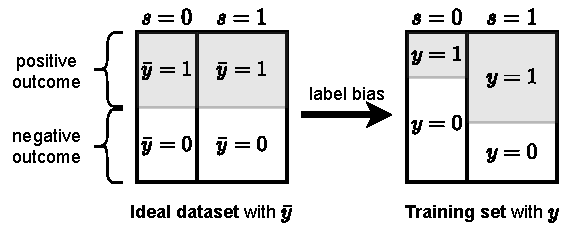
\includegraphics[width=0.9\textwidth]{figures/label_bias.pdf}
  \caption{%
    A diagram of a simple case of label bias, where both the class label \(y\) and the sensitive attribute \(s\) are binary.
    On the left, we have the ideal (possibly fictional) dataset with the target labels \(\bar{y}\),
    where the proportion of positive outcomes is the same for both demographic groups;
    and on the right, the training labels, for which the proportions are \emph{not} the same.
  }%
  \label{fig:label-bias-overview}
\end{figure}

We can interpret the contributions of this publication in two ways.
The first corresponds to the definition-centric view of dataset bias,
and the second to the ground-truth-centric view.
\begin{enumerate}
  \item
    We can say that the classifier should satisfy demographic parity in its predictions,
    and learning from a balanced training set is just one particular way to achieve this.
    In this view, the pseudo labels have no deeper meaning and are just a computational trick.
  \item
    We can see the training set as a corrupted version of a true dataset, which is balanced (\(y\perp s\)),
    and so, by learning from these pseudo labels, we are simply approximating the true dataset.
    However, we do not actually have access to the true dataset; we only know that it is balanced.
    In order to evaluate the trained model, we compute fairness metrics with respect to \ac{DP}.
\end{enumerate}
Within the paper, we sometimes jump between these two views.

While the main focus is on label bias,
the experiments are performed on real-world fairness datasets,
which also display a significant amount of sample bias (disadvantaged groups are underrepresented).
Furthermore, in addition to the result for \ac{DP}, we also show that the proposed scheme improves \acf{EOpp}.

In order to construct the target labels,
we use side information about summary statistics for a balanced training set.
This allows us to target a specific balanced set, instead of just any balanced set.
In other words, rather than just enforcing \ac{DP}, the method gives control over the target rates \(P(\hat{y}=1|s)\),
which are the only fairness-hyperparameters of the model.
The target labels \(\bar{y}\) represent an uncertain estimate of labels corresponding to a balanced dataset
(one where \(\bar{y} \perp s\); see also \figref{fig:label-bias-overview}).
The idea is then the learn a predictor for these target labels instead of the given (biased) training labels \(y\).
Via the sum rule of probabilities, it is possible to express the model likelihood in terms of the target labels,
such that maximising the likelihood corresponds to improving the prediction of the target labels.

The requirements for the model are that it outputs probabilities
and that they are well-calibrated --
which means that for those samples
that the model predicts a 10\% chance of having a positive label (\(y=1\))
about 10\% in fact have a positive label,
and analogously for all other predicted probabilities.
The probabilities are needed for calculating the expected target label,
and the calibration ensures that this expectation is sensible.
Thus, we picked a \acf{GP} model as one model for the experiments,
as they have a reputation for being well-calibrated.
However, they come with the downside that they are (at least in their standard form)
not well-suited to very high dimensional data like images.
As such, we also construct a model based on \acf{LR}.

The method is validated with experiments
on the UCI Adult Income dataset and the ProPublica/COMPAS dataset,
which have been mentioned several times in \chapref{ch:related-work},
and which are the most common tabular fairness datasets.
While both these datasets comprise only tabular data,
there is nothing in principle that stops this method from being used for other kinds of data.
The choice to use these datasets and not others
was predominantly made for easier comparison to baselines,
and shorter experiment runtime.

\section{Overcoming severe sampling bias with a representative set}\label{sec:nifr}
In the setting from the above paper \citep{kehrenberg2020tuning},
labels were untrustworthy because they had been flipped;
a phenomenon we referred to as \emph{label bias}.
However, flipping labels is not the only way that labels can become untrustworthy.
Another way is \emph{sampling bias}, which is the subject of \citet{kehrenberg2020nullsampling} and \citet{kehrenberg2020zeroshot} (\twochaprefs{ch:paper2}{ch:paper3}).

As an example, consider the scenario where someone wants to create a classifier
to distinguish between sheep and cows, that is supposed to work anywhere on earth.
However, they take a shortcut while creating the dataset
and take all their sheep images from hot and dry countries
and all their cow images from mild and rainy countries.
In this case, the dataset is lacking cow images in dry landscapes,
and is lacking sheep from green landscapes;
the dataset exhibits a strong sampling bias.
The result is that even though the labels correctly correspond to cows and sheep,
they do not point reliably to the right target anymore.
As background colour is easier to recognise with a \ac{CNN} than animal species,
the labels have effectively been turned into landscape labels.
In other words, landscape has become a \emph{spurious attribute}.
%
% As an example, consider a dataset where the task is to distinguish smiling from non-smiling faces.
% Say, we initially have a very diverse and balanced training set,
% but then, from the set of smiling faces, we remove nearly all samples where the person does not have red hair,
% and from the set of non-smiling faces, we remove nearly all samples with non-black hair.
% The result is that even though the labels are still correct, they do not point reliably to the right target anymore.
% As hair colour is easier to recognise with a \ac{CNN}, the labels have effectively been turned into hair colour labels.
% In other words, hair colour has become a \emph{spurious attribute}.
In the following, we denote the spurious attribute with \(s\),
as it takes on a role that is very similar to that of the sensitive attribute that was also denoted by \(s\).
However, there is a difference in emphasis between a \emph{sensitive} and a \emph{spurious} attribute:
the former indicates that the attribute should not be used for legal or ethical reasons,
whereas the latter can be any attribute that is associated with the class label \(y\) in an undesired way
that leads to lower quality generalisation.

The method, proposed in the previous paper (\chapref{ch:paper1}),
is not able to deal with such a dataset bias as we can easily see:
Say, \emph{smiling} corresponds to \(y=1\) and \emph{not smiling} to \(y=0\);
furthermore, let red hair correspond to \(s=1\), black hair to \(s=0\), and all other hair colours to \(s=2\).
Then, the problem with the described dataset is, that it mostly consists of samples with \(y=0\wedge s=0\)
and those with \(y=1\wedge s=1\).
If we call \(P(y=1|s=s')\) the acceptance rate,
then the problem can be described as one of very different acceptance rates in the hair colour groups given by \(s\).
This is the problem tackled in the previous paper,
and yet, if we were to equalise the acceptance rates with the method there,
the result would be very incorrect.
The issue is that we would treat the labels as incorrect, when in truth, they are correct;
the problem with the data being sampling bias.

To deal with sampling bias, a different approach is needed.
Indeed, the problem, as posed, is not solvable in the general case.
To make headway with this problem, we introduce the concept of a \emph{representative set}.
This set is not subject to the sampling bias,
but is unlabelled (with respect to $y$) and so does not by itself suffice for training.
However, this set does have labels for the spurious attribute \(s\).
This allows us to learn an \emph{invariant representation},
\ie, a representation of the input features \(x\) which is invariant to the spurious attribute.
This kind of representation is equivalent to a fair representation -- as described in \secref{sec:fair-representation} --
which is invariant to a sensitive attribute.
With the invariant representation of the training set,
a classifier can then be trained to accurately predict the class label \(y\).
The invariant representation cannot be learned from the training set
because there, due to the sampling bias, \(s\) and \(y\) are not sufficiently distinguishable.

A parallel to the previous paper is that the method makes use of side information
(in this case the representative set)
in order to overcome the bias in the training set.

The method implementing this general strategy, and presented in \citet{kehrenberg2020nullsampling} (\chapref{ch:paper2}),
is based on the idea of \emph{null-sampling},
which refers to zeroing out part of an encoding,
and then reconstructing the modified encoding as if it were a normal encoding.
In order to apply null-sampling, an encoding of the input \(x\) is learned that is split into two parts:
\(z_u\), which has no information about the spurious attribute \(s\),
and \(z_b\), which has all the remaining information needed to reconstruct \(x\) that is not contained in \(z_u\).
\(z_u\) is ensured to be not predictive of \(s\) via adversarial training.
During null-sampling, \(z_b\) is zeroed out, and after decoding it,
we obtain an invariant representation \emph{in the data domain}.
The fact that it is in the data domain makes it interpretable (or inspectable)
as defined in \chapref{ch:introduction}.

The described method works particularly well with \acp{INN},
as they ensure that no information is lost that is unrelated to \(s\).
However, the price to pay for using \acp{INN} is higher memory requirement and slower training.
Thus, we also present a variant of the method using \iac{VAE},
which does not have the guarantee about preserving information,
but also does not suffer from the increased training cost as much.
\acp{VAE} are similar to \acp{INN}
in that their encoding conforms to a specific probability distribution,
from which we can sample our null-samples.
The choice between the two presented variants is determined
by whether the user is willing to accept higher training costs
for a lower probability of losing information needed for any prediction tasks.
However, the key element is simply any kind of encoder -- producing a split-encoding --
whose output can be subjected to adversarial training,
so encoders other than \acp{VAE} or \acp{INN} will potentially work as well.

We perform experiments on the Coloured MNIST dataset (as described in \secref{sec:groundtruth-centric-view-of-bias}),
which has a one-to-one mapping between the class label (\ie, digit) and the spurious attribute (colour)
in the training set.
As colour is ``easier'' to learn, a neural network will learn to predict \(s\) instead of \(y\).
For additional experiments on the CelebA dataset (another image dataset)
and the UCI Adult Income dataset (a tabular dataset),
we deliberately apply sampling bias to the training set and then apply our method.
For the tabular dataset, an autoencoder is trained to produce a continuous representation,
which is then fed into the \ac{INN} or \ac{VAE} model.
Thus, we demonstrate that the method is \emph{general}
in the sense that it is applicable to both image-based and tabular datasets
and furthermore should be applicable to other modalities as well.
For the main experiments, we focus on image datasets,
because they are easiest to visualise in a document.

\section{Overcoming sampling bias with an unlabelled deployment set}\label{sec:zsf}
A shortcoming of the approach from the previous publication \citep{kehrenberg2020nullsampling}
is its reliance on a representative set which has labels for the spurious attribute \(s\).
As discussed, it is necessary to make use of \emph{some} kind of side information,
but perhaps we can relax some requirements.
In particular, while it is already easier to collect data without \(y\) labels (but with \(s\) labels),
it is even easier to collect data without \emph{any} label.
Thus, requiring only an unlabelled context set would improve the applicability of the method.
\citet{kehrenberg2020zeroshot} (\chapref{ch:paper3}) presents an approach based on that idea.

The setting is very similar to the previous publication \citep{kehrenberg2020nullsampling}:
the training set suffers from severe sampling bias, but we have access to a (mostly) unbiased \emph{deployment set}
(similar to but not quite identical to the previously discussed \emph{representative set}).
The idea is that the deployment set corresponds to the setting in which the model is meant to be deployed.
The change from the previous setting is that this additional set may be completely unlabelled,
but in exchange, we have some stronger requirements for the training set:
The holes left by the sampling bias may not be so numerous
as to make \(s\) and \(y\) completely indistinguishable.
For example, in the previous work, the example of Coloured MNIST had a training set
where there was a strict one-to-one mapping of colour and digit;
but this kind of blending of \(s\) and \(y\) into one is not the focus of this paper.
Instead, the focus is on a setting where the training set lacks certain combinations of \(s\) and \(y\),
which results in poor predictions for these combinations on the test set (or deployment setting)
where those combinations \emph{do} occur.
We refer to these missing combinations as \emph{subgroup bias} or \emph{missing subgroups},
depending on whether a given \(s\) value appears in the training set at all.
The label \(s\) plays here a similar role to the spurious attribute in the previous publication,
but as there is a change in emphasis, we refer to \(s\) as \emph{subgroup label}%
\footnote{This terminology is inspired by the \emph{subclass} concept in \citet{SohDunAngGuetal20}.}
instead.
The difference between a spurious attribute and a subgroup label is that
the former is mostly characterised via its confusion with the prediction target,
whereas the latter refers to natural groups in the data
which have differing levels of annotation quality which affects the classification performance on these subgroups.
However, in both cases, the goal is to make the model output invariant to the \(s\) label,
\ie the classification performance should be independent of the subgroup.

As in the previous paper, the first step is to train a neural network to produce an invariant representation.
The second step is then to train a classifier on said representation.
The invariant representation is trained by performing \emph{distribution matching} between the training set and the deployment set.
% Finally, the training set is transformed into the invariant representation,
% to serve as training set for the classifier.

The distribution matching is realised with adversarial networks which compare batches of samples,
in order to try to distinguish data drawn from the training set and the deployment set.
This process requires balanced batches as an inductive bias,
because the network will only learn the intended difference between training and deployment set,
if the drawn batches exhibit this difference.
For example, if batches drawn from Coloured MNIST differ not in colour but in digit class,
then distribution matching will learn to change digit shapes.
Balancing batches from the training set is easily possible with the available labels,
but those are not available for the deployment set,
so we use clustering techniques to identify the different groups in the deployment set,
and then draw samples for the batches at an equal rate from all clusters.
It is important to note here that imperfections in the clustering are not a problem
as long as the batches show on average the intended difference between training and deployment set.

The absolutely essential elements for this method are the encoder (also referred to as `de-biaser')
that encodes both, samples from the training set and samples from the deployment set,
to a splittable representation;
the adversary that tries to identify, from one part of the split representation,
which dataset the given samples originated from;
and some kind of reconstruction loss
to ensure the splittable representation represents the input data well.
The following elements are in theory optional,
but are needed for the method to work with real-world data:
clustering and sampling to ensure that the training batches are balanced in specific ways;
subdivision of the batches into bags; and the aggregation of the adversarial loss over the bags.
Roughly speaking, these elements strengthen the supervision signal for the invariance learning.

Experiments are performed on the same datasets as in the previous papers:
Coloured MNIST, UCI Adult Income and CelebA.
Again, these datasets were chosen, because image data is easy to visualise,
and because demonstrating the method on tabular data provides evidence for the generality.

% \section{Claims and contributions}%
\section{List of publications and author contributions}%
\label{sec:claims-contributions}
This thesis is based on 3 publications (one of which is a work in progress),
corresponding to \rangechapref{ch:paper1}{ch:paper3}.
% The first one is concerned with \emph{label bias} and the other two with \emph{sampling bias}.
The following is a detailed listing of all the individual author contributions.

\subsection{Publication 1}
\begin{refsection}[allreferences]
    \nocite{kehrenberg2020tuning}
    \printbibliography[heading=none]
\end{refsection}
\noindent A shorter version was published as a workshop paper:
\begin{refsection}[allreferences]
    \nocite{kehrenberg2018interpretable}
    \printbibliography[heading=none]
\end{refsection}
\noindent\textsc{Contributions:}
\begin{itemize}
  \item I conceived the idea of using Target Labels to target a balanced set.
    I developed the proof from a starting point that my supervisor pointed me to.
    I wrote all of the code dealing with the modified loss function and nearly all of the remaining code as well.
    I ran most of the experiments and wrote all of the methods section and most of the remaining text as well.
  \item Z. Chen was a discussion partner and helped run the experiments, and wrote some parts of the code.
  \item N. Quadrianto suggested the initial direction of the work, was a discussion partner,
    and helped write the introduction and related work.
\end{itemize}

\subsection{Publication 2}
\begin{refsection}[allreferences]
    \nocite{kehrenberg2020nullsampling}
    \printbibliography[heading=none]
\end{refsection}%
\noindent\textsc{Contributions:}
\begin{itemize}
  \item I conceived the idea of using an \acf{INN} and a representative set to learn an invariant representation.
    I wrote a large part of the code, and ran about half the experiments. I wrote a significant part of the text.
  \item M. Bartlett developed a large part of the tricks needed for training the \ac{INN} successfully.
    He wrote a significant part of the code, and of the text.
  \item O. Thomas helped with writing the code and with running the experiments.
  \item N. Quadrianto gave feedback on the progress and suggested directions to explore.
\end{itemize}

\subsection{Publication 3 (work in progress)}
\begin{refsection}[allreferences]
    \nocite{kehrenberg2020zeroshot}
    \printbibliography[heading=none]
\end{refsection}%
\noindent\textsc{Contributions:}
\begin{itemize}
  \item I developed the idea of distribution matching as an extension of the previous paper.
    In addition, I tried to achieve similar goals by applying clustering to an unlabelled auxiliary set,
    with supervision from the labelled training set.
    I wrote all of the initial implementation of the method, and a large part of the later refined implementation.
    I ran the majority of the experiments.
  \item V. Sharmanska developed the original link to a fairness problem
    and wrote parts of the introduction and related work and contributed to other sections.
  \item M. Bartlett introduced the idea of batches-of-bags.
    He also improved the \ac{NN} architectures of the encoder and the discriminator,
    ran experiments, wrote the sections on architecture and contributed to other parts of the paper.
  \item N. Quadrianto suggested how to combine the two research directions that I had into a coherent whole.
    He also gave general feedback and suggested directions to explore.
\end{itemize}


\cleardoublepage
\ctparttext{
  This part comprises two peer-reviewed publications and one submitted paper currently under review.
  They are reproduced here with minimal changes.
}
\part{Publications}\label{pt:main}
% \documentclass{article}
% \usepackage{style}
% \usepackage{times}

% %%%%% NEW MATH DEFINITIONS %%%%%

\usepackage{amsmath,amsfonts,bm}

% Mark sections of captions for referring to divisions of figures
\newcommand{\figleft}{{\em (Left)}}
\newcommand{\figcenter}{{\em (Center)}}
\newcommand{\figright}{{\em (Right)}}
\newcommand{\figtop}{{\em (Top)}}
\newcommand{\figbottom}{{\em (Bottom)}}
\newcommand{\captiona}{{\em (a)}}
\newcommand{\captionb}{{\em (b)}}
\newcommand{\captionc}{{\em (c)}}
\newcommand{\captiond}{{\em (d)}}

% Highlight a newly defined term
\newcommand{\newterm}[1]{{\bf #1}}


% Figure reference, lower-case.
\def\figref#1{figure~\ref{#1}}
% Figure reference, capital. For start of sentence
\def\Figref#1{Figure~\ref{#1}}
\def\twofigref#1#2{figures \ref{#1} and \ref{#2}}
\def\quadfigref#1#2#3#4{figures \ref{#1}, \ref{#2}, \ref{#3} and \ref{#4}}
% Section reference, lower-case.
\def\secref#1{section~\ref{#1}}
% Section reference, capital.
\def\Secref#1{Section~\ref{#1}}
% Reference to two sections.
\def\twosecrefs#1#2{sections \ref{#1} and \ref{#2}}
% Reference to three sections.
\def\secrefs#1#2#3{sections \ref{#1}, \ref{#2} and \ref{#3}}
% Appendix reference, lower-case.
\def\appref#1{appendix~\ref{#1}}
% Appendix reference, capital.
\def\Appref#1{Appendix~\ref{#1}}
% Reference to an equation, lower-case.
\def\eqref#1{equation~\ref{#1}}
% Reference to an equation, upper case
\def\Eqref#1{Equation~\ref{#1}}
% A raw reference to an equation---avoid using if possible
\def\plaineqref#1{\ref{#1}}
% Reference to a chapter, lower-case.
\def\chapref#1{chapter~\ref{#1}}
% Reference to a Chapter, upper case.
\def\Chapref#1{Chapter~\ref{#1}}
\def\twochaprefs#1#2{chapters \ref{#1} and \ref{#2}}
% Reference to a range of chapters
\def\rangechapref#1#2{chapters \ref{#1}--\ref{#2}}
% Reference to a range of chapters, upper case
\def\Rangechapref#1#2{Chapters \ref{#1}--\ref{#2}}
% Reference to an algorithm, lower-case.
\def\algref#1{algorithm~\ref{#1}}
% Reference to an algorithm, upper case.
\def\Algref#1{Algorithm~\ref{#1}}
\def\twoalgref#1#2{algorithms \ref{#1} and \ref{#2}}
\def\Twoalgref#1#2{Algorithms \ref{#1} and \ref{#2}}
% Reference to a part, lower case
\def\partref#1{part~\ref{#1}}
% Reference to a part, upper case
\def\Partref#1{Part~\ref{#1}}
\def\twopartref#1#2{parts \ref{#1} and \ref{#2}}

\def\ceil#1{\lceil #1 \rceil}
\def\floor#1{\lfloor #1 \rfloor}
\def\1{\bm{1}}
\newcommand{\train}{\mathcal{D}}
\newcommand{\valid}{\mathcal{D_{\mathrm{valid}}}}
\newcommand{\test}{\mathcal{D_{\mathrm{test}}}}

\def\eps{{\epsilon}}


% Random variables
\def\reta{{\textnormal{$\eta$}}}
\def\ra{{\textnormal{a}}}
\def\rb{{\textnormal{b}}}
\def\rc{{\textnormal{c}}}
\def\rd{{\textnormal{d}}}
\def\re{{\textnormal{e}}}
\def\rf{{\textnormal{f}}}
\def\rg{{\textnormal{g}}}
\def\rh{{\textnormal{h}}}
\def\ri{{\textnormal{i}}}
\def\rj{{\textnormal{j}}}
\def\rk{{\textnormal{k}}}
\def\rl{{\textnormal{l}}}
% rm is already a command, just don't name any random variables m
\def\rn{{\textnormal{n}}}
\def\ro{{\textnormal{o}}}
\def\rp{{\textnormal{p}}}
\def\rq{{\textnormal{q}}}
\def\rr{{\textnormal{r}}}
\def\rs{{\textnormal{s}}}
\def\rt{{\textnormal{t}}}
\def\ru{{\textnormal{u}}}
\def\rv{{\textnormal{v}}}
\def\rw{{\textnormal{w}}}
\def\rx{{\textnormal{x}}}
\def\ry{{\textnormal{y}}}
\def\rz{{\textnormal{z}}}

% Random vectors
\def\rvepsilon{{\mathbf{\epsilon}}}
\def\rvtheta{{\mathbf{\theta}}}
\def\rva{{\mathbf{a}}}
\def\rvb{{\mathbf{b}}}
\def\rvc{{\mathbf{c}}}
\def\rvd{{\mathbf{d}}}
\def\rve{{\mathbf{e}}}
\def\rvf{{\mathbf{f}}}
\def\rvg{{\mathbf{g}}}
\def\rvh{{\mathbf{h}}}
\def\rvu{{\mathbf{i}}}
\def\rvj{{\mathbf{j}}}
\def\rvk{{\mathbf{k}}}
\def\rvl{{\mathbf{l}}}
\def\rvm{{\mathbf{m}}}
\def\rvn{{\mathbf{n}}}
\def\rvo{{\mathbf{o}}}
\def\rvp{{\mathbf{p}}}
\def\rvq{{\mathbf{q}}}
\def\rvr{{\mathbf{r}}}
\def\rvs{{\mathbf{s}}}
\def\rvt{{\mathbf{t}}}
\def\rvu{{\mathbf{u}}}
\def\rvv{{\mathbf{v}}}
\def\rvw{{\mathbf{w}}}
\def\rvx{{\mathbf{x}}}
\def\rvy{{\mathbf{y}}}
\def\rvz{{\mathbf{z}}}

% Elements of random vectors
\def\erva{{\textnormal{a}}}
\def\ervb{{\textnormal{b}}}
\def\ervc{{\textnormal{c}}}
\def\ervd{{\textnormal{d}}}
\def\erve{{\textnormal{e}}}
\def\ervf{{\textnormal{f}}}
\def\ervg{{\textnormal{g}}}
\def\ervh{{\textnormal{h}}}
\def\ervi{{\textnormal{i}}}
\def\ervj{{\textnormal{j}}}
\def\ervk{{\textnormal{k}}}
\def\ervl{{\textnormal{l}}}
\def\ervm{{\textnormal{m}}}
\def\ervn{{\textnormal{n}}}
\def\ervo{{\textnormal{o}}}
\def\ervp{{\textnormal{p}}}
\def\ervq{{\textnormal{q}}}
\def\ervr{{\textnormal{r}}}
\def\ervs{{\textnormal{s}}}
\def\ervt{{\textnormal{t}}}
\def\ervu{{\textnormal{u}}}
\def\ervv{{\textnormal{v}}}
\def\ervw{{\textnormal{w}}}
\def\ervx{{\textnormal{x}}}
\def\ervy{{\textnormal{y}}}
\def\ervz{{\textnormal{z}}}

% Random matrices
\def\rmA{{\mathbf{A}}}
\def\rmB{{\mathbf{B}}}
\def\rmC{{\mathbf{C}}}
\def\rmD{{\mathbf{D}}}
\def\rmE{{\mathbf{E}}}
\def\rmF{{\mathbf{F}}}
\def\rmG{{\mathbf{G}}}
\def\rmH{{\mathbf{H}}}
\def\rmI{{\mathbf{I}}}
\def\rmJ{{\mathbf{J}}}
\def\rmK{{\mathbf{K}}}
\def\rmL{{\mathbf{L}}}
\def\rmM{{\mathbf{M}}}
\def\rmN{{\mathbf{N}}}
\def\rmO{{\mathbf{O}}}
\def\rmP{{\mathbf{P}}}
\def\rmQ{{\mathbf{Q}}}
\def\rmR{{\mathbf{R}}}
\def\rmS{{\mathbf{S}}}
\def\rmT{{\mathbf{T}}}
\def\rmU{{\mathbf{U}}}
\def\rmV{{\mathbf{V}}}
\def\rmW{{\mathbf{W}}}
\def\rmX{{\mathbf{X}}}
\def\rmY{{\mathbf{Y}}}
\def\rmZ{{\mathbf{Z}}}

% Elements of random matrices
\def\ermA{{\textnormal{A}}}
\def\ermB{{\textnormal{B}}}
\def\ermC{{\textnormal{C}}}
\def\ermD{{\textnormal{D}}}
\def\ermE{{\textnormal{E}}}
\def\ermF{{\textnormal{F}}}
\def\ermG{{\textnormal{G}}}
\def\ermH{{\textnormal{H}}}
\def\ermI{{\textnormal{I}}}
\def\ermJ{{\textnormal{J}}}
\def\ermK{{\textnormal{K}}}
\def\ermL{{\textnormal{L}}}
\def\ermM{{\textnormal{M}}}
\def\ermN{{\textnormal{N}}}
\def\ermO{{\textnormal{O}}}
\def\ermP{{\textnormal{P}}}
\def\ermQ{{\textnormal{Q}}}
\def\ermR{{\textnormal{R}}}
\def\ermS{{\textnormal{S}}}
\def\ermT{{\textnormal{T}}}
\def\ermU{{\textnormal{U}}}
\def\ermV{{\textnormal{V}}}
\def\ermW{{\textnormal{W}}}
\def\ermX{{\textnormal{X}}}
\def\ermY{{\textnormal{Y}}}
\def\ermZ{{\textnormal{Z}}}

% Vectors
\def\vzero{{\bm{0}}}
\def\vone{{\bm{1}}}
\def\vmu{{\bm{\mu}}}
\def\vtheta{{\bm{\theta}}}
\def\va{{\bm{a}}}
\def\vb{{\bm{b}}}
\def\vc{{\bm{c}}}
\def\vd{{\bm{d}}}
\def\ve{{\bm{e}}}
\def\vf{{\bm{f}}}
\def\vg{{\bm{g}}}
\def\vh{{\bm{h}}}
\def\vi{{\bm{i}}}
\def\vj{{\bm{j}}}
\def\vk{{\bm{k}}}
\def\vl{{\bm{l}}}
\def\vm{{\bm{m}}}
\def\vn{{\bm{n}}}
\def\vo{{\bm{o}}}
\def\vp{{\bm{p}}}
\def\vq{{\bm{q}}}
\def\vr{{\bm{r}}}
\def\vs{{\bm{s}}}
\def\vt{{\bm{t}}}
\def\vu{{\bm{u}}}
\def\vv{{\bm{v}}}
\def\vw{{\bm{w}}}
\def\vx{{\bm{x}}}
\def\vy{{\bm{y}}}
\def\vz{{\bm{z}}}

% Elements of vectors
\def\evalpha{{\alpha}}
\def\evbeta{{\beta}}
\def\evepsilon{{\epsilon}}
\def\evlambda{{\lambda}}
\def\evomega{{\omega}}
\def\evmu{{\mu}}
\def\evpsi{{\psi}}
\def\evsigma{{\sigma}}
\def\evtheta{{\theta}}
\def\eva{{a}}
\def\evb{{b}}
\def\evc{{c}}
\def\evd{{d}}
\def\eve{{e}}
\def\evf{{f}}
\def\evg{{g}}
\def\evh{{h}}
\def\evi{{i}}
\def\evj{{j}}
\def\evk{{k}}
\def\evl{{l}}
\def\evm{{m}}
\def\evn{{n}}
\def\evo{{o}}
\def\evp{{p}}
\def\evq{{q}}
\def\evr{{r}}
\def\evs{{s}}
\def\evt{{t}}
\def\evu{{u}}
\def\evv{{v}}
\def\evw{{w}}
\def\evx{{x}}
\def\evy{{y}}
\def\evz{{z}}

% Matrix
\def\mA{{\bm{A}}}
\def\mB{{\bm{B}}}
\def\mC{{\bm{C}}}
\def\mD{{\bm{D}}}
\def\mE{{\bm{E}}}
\def\mF{{\bm{F}}}
\def\mG{{\bm{G}}}
\def\mH{{\bm{H}}}
\def\mI{{\bm{I}}}
\def\mJ{{\bm{J}}}
\def\mK{{\bm{K}}}
\def\mL{{\bm{L}}}
\def\mM{{\bm{M}}}
\def\mN{{\bm{N}}}
\def\mO{{\bm{O}}}
\def\mP{{\bm{P}}}
\def\mQ{{\bm{Q}}}
\def\mR{{\bm{R}}}
\def\mS{{\bm{S}}}
\def\mT{{\bm{T}}}
\def\mU{{\bm{U}}}
\def\mV{{\bm{V}}}
\def\mW{{\bm{W}}}
\def\mX{{\bm{X}}}
\def\mY{{\bm{Y}}}
\def\mZ{{\bm{Z}}}
\def\mBeta{{\bm{\beta}}}
\def\mPhi{{\bm{\Phi}}}
\def\mLambda{{\bm{\Lambda}}}
\def\mSigma{{\bm{\Sigma}}}

% % Tensor
% \DeclareMathAlphabet{\mathsfit}{\encodingdefault}{\sfdefault}{m}{sl}
% \SetMathAlphabet{\mathsfit}{bold}{\encodingdefault}{\sfdefault}{bx}{n}
% \newcommand{\tens}[1]{\bm{\mathsfit{#1}}}
% \def\tA{{\tens{A}}}
% \def\tB{{\tens{B}}}
% \def\tC{{\tens{C}}}
% \def\tD{{\tens{D}}}
% \def\tE{{\tens{E}}}
% \def\tF{{\tens{F}}}
% \def\tG{{\tens{G}}}
% \def\tH{{\tens{H}}}
% \def\tI{{\tens{I}}}
% \def\tJ{{\tens{J}}}
% \def\tK{{\tens{K}}}
% \def\tL{{\tens{L}}}
% \def\tM{{\tens{M}}}
% \def\tN{{\tens{N}}}
% \def\tO{{\tens{O}}}
% \def\tP{{\tens{P}}}
% \def\tQ{{\tens{Q}}}
% \def\tR{{\tens{R}}}
% \def\tS{{\tens{S}}}
% \def\tT{{\tens{T}}}
% \def\tU{{\tens{U}}}
% \def\tV{{\tens{V}}}
% \def\tW{{\tens{W}}}
% \def\tX{{\tens{X}}}
% \def\tY{{\tens{Y}}}
% \def\tZ{{\tens{Z}}}


% Graph
\def\gA{{\mathcal{A}}}
\def\gB{{\mathcal{B}}}
\def\gC{{\mathcal{C}}}
\def\gD{{\mathcal{D}}}
\def\gE{{\mathcal{E}}}
\def\gF{{\mathcal{F}}}
\def\gG{{\mathcal{G}}}
\def\gH{{\mathcal{H}}}
\def\gI{{\mathcal{I}}}
\def\gJ{{\mathcal{J}}}
\def\gK{{\mathcal{K}}}
\def\gL{{\mathcal{L}}}
\def\gM{{\mathcal{M}}}
\def\gN{{\mathcal{N}}}
\def\gO{{\mathcal{O}}}
\def\gP{{\mathcal{P}}}
\def\gQ{{\mathcal{Q}}}
\def\gR{{\mathcal{R}}}
\def\gS{{\mathcal{S}}}
\def\gT{{\mathcal{T}}}
\def\gU{{\mathcal{U}}}
\def\gV{{\mathcal{V}}}
\def\gW{{\mathcal{W}}}
\def\gX{{\mathcal{X}}}
\def\gY{{\mathcal{Y}}}
\def\gZ{{\mathcal{Z}}}

% Sets
\def\sA{{\mathbb{A}}}
\def\sB{{\mathbb{B}}}
\def\sC{{\mathbb{C}}}
\def\sD{{\mathbb{D}}}
% Don't use a set called E, because this would be the same as our symbol
% for expectation.
\def\sF{{\mathbb{F}}}
\def\sG{{\mathbb{G}}}
\def\sH{{\mathbb{H}}}
\def\sI{{\mathbb{I}}}
\def\sJ{{\mathbb{J}}}
\def\sK{{\mathbb{K}}}
\def\sL{{\mathbb{L}}}
\def\sM{{\mathbb{M}}}
\def\sN{{\mathbb{N}}}
\def\sO{{\mathbb{O}}}
\def\sP{{\mathbb{P}}}
\def\sQ{{\mathbb{Q}}}
\def\sR{{\mathbb{R}}}
\def\sS{{\mathbb{S}}}
\def\sT{{\mathbb{T}}}
\def\sU{{\mathbb{U}}}
\def\sV{{\mathbb{V}}}
\def\sW{{\mathbb{W}}}
\def\sX{{\mathbb{X}}}
\def\sY{{\mathbb{Y}}}
\def\sZ{{\mathbb{Z}}}

% Entries of a matrix
\def\emLambda{{\Lambda}}
\def\emA{{A}}
\def\emB{{B}}
\def\emC{{C}}
\def\emD{{D}}
\def\emE{{E}}
\def\emF{{F}}
\def\emG{{G}}
\def\emH{{H}}
\def\emI{{I}}
\def\emJ{{J}}
\def\emK{{K}}
\def\emL{{L}}
\def\emM{{M}}
\def\emN{{N}}
\def\emO{{O}}
\def\emP{{P}}
\def\emQ{{Q}}
\def\emR{{R}}
\def\emS{{S}}
\def\emT{{T}}
\def\emU{{U}}
\def\emV{{V}}
\def\emW{{W}}
\def\emX{{X}}
\def\emY{{Y}}
\def\emZ{{Z}}
\def\emSigma{{\Sigma}}

% entries of a tensor
% Same font as tensor, without \bm wrapper
% \newcommand{\etens}[1]{\mathsfit{#1}}
% \def\etLambda{{\etens{\Lambda}}}
% \def\etA{{\etens{A}}}
% \def\etB{{\etens{B}}}
% \def\etC{{\etens{C}}}
% \def\etD{{\etens{D}}}
% \def\etE{{\etens{E}}}
% \def\etF{{\etens{F}}}
% \def\etG{{\etens{G}}}
% \def\etH{{\etens{H}}}
% \def\etI{{\etens{I}}}
% \def\etJ{{\etens{J}}}
% \def\etK{{\etens{K}}}
% \def\etL{{\etens{L}}}
% \def\etM{{\etens{M}}}
% \def\etN{{\etens{N}}}
% \def\etO{{\etens{O}}}
% \def\etP{{\etens{P}}}
% \def\etQ{{\etens{Q}}}
% \def\etR{{\etens{R}}}
% \def\etS{{\etens{S}}}
% \def\etT{{\etens{T}}}
% \def\etU{{\etens{U}}}
% \def\etV{{\etens{V}}}
% \def\etW{{\etens{W}}}
% \def\etX{{\etens{X}}}
% \def\etY{{\etens{Y}}}
% \def\etZ{{\etens{Z}}}

% The true underlying data generating distribution
\newcommand{\pdata}{p_{\rm{data}}}
% The empirical distribution defined by the training set
\newcommand{\ptrain}{\hat{p}_{\rm{data}}}
\newcommand{\Ptrain}{\hat{P}_{\rm{data}}}
% The model distribution
\newcommand{\pmodel}{p_{\rm{model}}}
\newcommand{\Pmodel}{P_{\rm{model}}}
\newcommand{\ptildemodel}{\tilde{p}_{\rm{model}}}
% Stochastic autoencoder distributions
\newcommand{\pencode}{p_{\rm{encoder}}}
\newcommand{\pdecode}{p_{\rm{decoder}}}
\newcommand{\precons}{p_{\rm{reconstruct}}}

\newcommand{\laplace}{\mathrm{Laplace}} % Laplace distribution

\newcommand{\E}{\mathbb{E}}
\newcommand{\Ls}{\mathcal{L}}
\newcommand{\R}{\mathbb{R}}
\newcommand{\emp}{\tilde{p}}
\newcommand{\lr}{\alpha}
\newcommand{\reg}{\lambda}
\newcommand{\rect}{\mathrm{rectifier}}
\newcommand{\softmax}{\mathrm{softmax}}
\newcommand{\sigmoid}{\sigma}
\newcommand{\softplus}{\zeta}
\newcommand{\KL}{D_{\mathrm{KL}}}
\newcommand{\Var}{\mathrm{Var}}
\newcommand{\standarderror}{\mathrm{SE}}
\newcommand{\Cov}{\mathrm{Cov}}
% Wolfram Mathworld says $L^2$ is for function spaces and $\ell^2$ is for vectors
% But then they seem to use $L^2$ for vectors throughout the site, and so does
% wikipedia.
\newcommand{\normlzero}{L^0}
\newcommand{\normlone}{L^1}
\newcommand{\normltwo}{L^2}
\newcommand{\normlp}{L^p}
\newcommand{\normmax}{L^\infty}

\newcommand{\parents}{Pa} % See usage in notation.tex. Chosen to match Daphne's book.

\DeclareMathOperator*{\argmax}{arg\,max}
\DeclareMathOperator*{\argmin}{arg\,min}

\DeclareMathOperator{\sign}{sign}
\DeclareMathOperator{\Tr}{Tr}
\let\ab\allowbreak


% \bibliographystyle{bibstyle}

% \usepackage{amssymb}
% \usepackage{amsmath}
% \usepackage{amsthm}
% \usepackage{bbm}
% \newtheorem{theorem}{Theorem}%[section]
% \newtheorem{corollary}{Corollary}[theorem]
% \newtheorem{lemma}[theorem]{Lemma}
% \theoremstyle{definition}
% \newtheorem{definition}{Definition}%[section]
% \newtheorem{example}{Example}%[section]

% \usepackage{tikz}
% \usetikzlibrary{arrows,positioning,shapes.misc}
% \usepackage{pgfplots} % for creating the graphs
% \pgfplotsset{compat=1.8}
% \usepackage{nicefrac}
% \usepackage{algorithm}
% \usepackage{algorithmic}
% \usepackage{xcolor}
% \usepackage{comment}
% \usepackage{booktabs}
% \usepackage{authblk}
% \usepackage{url,hyperref,microtype,subcaption}

% \author[1]{Thomas Kehrenberg}
% \author[1,2]{Zexun Chen}
% \author[1]{Novi Quadrianto}
% \affil[1]{Predictive Analytics Lab (PAL), University of Sussex, Brighton, UK}
% \affil[2]{BioComplex Laboratory, University of Exeter, Exeter, UK}
% \title{Tuning Fairness by Balancing Target Labels} 

% \newcommand{P}{\mathbb{P}} % Probability
% \renewcommand{\algorithmicrequire}{\textbf{Input:}}
% \renewcommand{\algorithmicensure}{\textbf{Output:}}
% \newcommand{\thomas}[1]{\textcolor{brown}{\textbf{Thomas:} #1}}
% \newcommand{\novi}[1]{\textcolor{red}{\textbf{Novi:} #1}}
% \newcommand{\myles}[1]{\textcolor{blue}{\textbf{Myles:} #1}}


% \iclrfinalcopy
% \begin{document}
% \maketitle

% ============= content ====================
\section{Abstract}

%%% Leave the Abstract empty if your article does not require one, please see the Summary Table for full details.
% \section{}
% For full guidelines regarding your manuscript please refer to \href{http://www.frontiersin.org/about/AuthorGuidelines}{Author Guidelines}.
% As a primary goal, the abstract should render the general significance and conceptual advance of the work clearly accessible to a broad readership. References should not be cited in the abstract. Leave the Abstract empty if your article does not require one, please see \href{http://www.frontiersin.org/about/AuthorGuidelines#SummaryTable}{Summary Table} for details according to article type. 
%
The issue of fairness in machine learning models has recently attracted a lot of attention as ensuring it will ensure continued confidence of the general public in the deployment of machine learning systems.
We focus on mitigating the harm incurred by a biased machine learning system
that offers better outputs (e.g.\ loans, job interviews) for certain groups than for others.
We show that bias in the output can naturally be controlled in probabilistic models
by introducing a latent target output. 
This formulation has several advantages:
first, it is a unified framework for several notions of group fairness such as Demographic Parity and Equality of Opportunity;
second, it is expressed as a marginalisation instead of a constrained problem;
and third, it allows the encoding of our knowledge of what unbiased outputs should be.
%
Practically, the second allows us to avoid unstable constrained optimisation procedures and to reuse off-the-shelf toolboxes.
%
The latter translates to the ability to control the level of fairness by
directly varying fairness target rates. %such as true positive rates and positive rates.
In contrast, existing approaches rely on intermediate, arguably unintuitive, control parameters such as covariance thresholds.
%We also develop a theory for Bayes-optimal classification with bias controlling mechanisms in terms of true positive rates and positive rates.

% \tiny
 % \keyFont{
 % \section{Keywords:} algorithmic bias, fairness, machine learning, demographic parity, equality of opportunity %All article types: you may provide up to 8 keywords; at least 5 are mandatory.

%Please also refer to  \href{http://home.frontiersin.org/about/author-guidelines#Sections}{Author Guidelines} for further information on how to organize your manuscript in the required sections or their equivalents for your field

% \subsection{Figures}
% Frontiers requires figures to be submitted individually, in the same order as they are referred to in the manuscript. Figures will then be automatically embedded at the bottom of the submitted manuscript. Kindly ensure that each table and figure is mentioned in the text and in numerical order. Figures must be of sufficient resolution for publication \href{http://home.frontiersin.org/about/author-guidelines#ResolutionRequirements}{see here for examples and minimum requirements}.
% Figures which are not according to the guidelines will cause substantial delay during the production process. Please see \href{http://home.frontiersin.org/about/author-guidelines#GeneralStyleGuidelinesforFigures}{here} for full figure guidelines. Cite figures with subfigures as figure \ref{fig:2}B.

% \subsection{Tables}
% Tables should be inserted at the end of the manuscript. Please build your table directly in LaTeX.Tables provided as jpeg/tiff files will not be accepted. Please note that very large tables (covering several pages) cannot be included in the final PDF for reasons of space.
% These tables will be published as \href{http://home.frontiersin.org/about/author-guidelines#SupplementaryMaterial}{Supplementary Material} on the online article page at the time of acceptance. The author will be notified during the typesetting of the final article if this is the case. 

\section{Introduction}
%\myles{need a punchier opening}
Algorithmic assessment methods are used for predicting human outcomes in areas such as financial services, recruitment, crime and justice, and local government.
This contributes, in theory, to a world with decreasing human biases.
To achieve this, however, we need fair machine learning models that take biased datasets,
but output non-discriminatory decisions to people with differing protected attributes such as gender and marital status.
Datasets can be biased because of, for example, sampling bias, subjective bias of individuals, and institutionalised biases \citep{OltCasDiaKic19,Tol19}.
Uncontrolled bias in the data can translate into bias in machine learning models.

There is no single accepted definition of algorithmic fairness for automated decision-making
but several have been proposed.
One definition is referred to as \emph{statistical} or \emph{demographic parity}.
Given a binary protected attribute (e.g.\ married/unmarried) and a binary decision (e.g.\ yes/no to getting a loan),
demographic parity requires equal positive rates (PR) across the two sensitive groups (married and \emph{un}married individuals should be equally likely to receive a loan).
%
Another fairness criterion, \emph{equalised odds}~\citep{hardt2016equality},
takes into account the binary decision, and instead of equal PR requires equal true positive rates (TPR) and false positive rates (FPR).
This criterion is intended to be more compatible with the goal of building accurate predictors or achieving high utility~\citep{hardt2016equality}.
We discuss the suitability of the different fairness criteria in the discussion section at the end of the paper.

There are many existing models for enforcing demographic parity and equalised odds
\citep{CreMadJacWeietal19,AgaBeyDudLanetal18,calders2009building,kamishima2012fairness,zafar2017fairnesstreatment,zafar2017fairnessconstraints}.
However, these existing approaches to balancing accuracy and fairness rely on intermediate, unintuitive control parameters such as allowable constraint violation $\epsilon$ (e.g. $0.01$) in \citet{AgaBeyDudLanetal18}, or a covariance threshold $c$
(e.g. $0$ that is controlled by another parameters $\tau$ and $\mu$ -- $0.005$ and $1.2$ -- to trade off this threshold and accuracy)
in \citet{zafar2017fairnesstreatment}.
This is related to the fact that many of these approaches embed fairness criteria as \emph{constraints} in the optimisation procedure
\citep{DonOneBenShaetal18,quadrianto2017recycling,zafar2017fairnesstreatment,zafar2017fairnessconstraints}.

In contrast, we provide a probabilistic classification framework with bias controlling mechanisms that can be tuned based on positive rates (PR),
an intuitive parameter.
Thus, giving humans the control to set the rate of positive predictions (e.g.\ a PR of $0.6$).
Our framework is based on the concept of a \emph{balanced dataset}
and introduces latent target labels, which, instead of the provided labels, are now the training label of our classifier.
We prove bounds on how far the target labels diverge from the dataset labels.
We instantiate our approach with a parametric logistic regression classifier and a Bayesian non-parametric Gaussian process classifier (GPC).
%
As our formulation is not expressed as a constrained problem,
we can draw upon advancements in automated variational inference~\citep{bonilla2016generic,gardner2018gpytorch,krauth2016autogp}
for learning the fair model, and for handling large amounts of data.

The method presented in this paper is closely related to a number of previous works,
e.g.\ \citet{kamiran2012data,calders2010three}.
Proper comparison with them requires knowledge of our approach.
We will thus explain our approach in the subsequent sections, and defer detailed comparisons to Section~\ref{sec:relatedwork} (Related Work).

\section{Target labels for tuning group fairness}
We will start by describing several notions of group fairness.
For each individual, we have a vector of non-sensitive attributes $x\in\mathcal{X}$, a class label $y\in\mathcal{Y}$, and a sensitive attribute $s\in\mathcal{S}$ (e.g.\ racial origin or gender).
%
We focus on the case where $s$ and $y$ are binary. 
%
We assume that a positive label $y=1$ corresponds to a positive outcome for an individual -- for example, being accepted for a loan.
%
%
\emph{Group fairness} balances a certain condition between groups of individuals with different sensitive attribute, $s$ versus $s\sp{\prime}$. 
%
The term $\hat{y}$ below is the prediction of a machine learning model that,
in most works, uses only non-sensitive attributes $x$.
%
Several group fairness criteria have been proposed (e.g. \citet{zafar2017fairnesstreatment,chouldechova2017fair,hardt2016equality}):
\begin{align}
& \text{equality of positive rate (Demographic Parity):}\nonumber\\
& \text{Pr}(\hat{y}=1|s)=\text{Pr}(\hat{y}=1|s\sp{\prime}) \label{eq:eq_dem_par}\\
& \text{equality of accuracy:}\nonumber\\
& \text{Pr}(\hat{y}=y|s)=\text{Pr}(\hat{y}=y|s\sp{\prime}) \\
& \text{equality of true positive rate (Equality of Opportunity):} \nonumber\\
& \text{Pr}(\hat{y}=1|s,y=1)=\text{Pr}(\hat{y}=1|s\sp{\prime},y=1)  \label{eq:eq_opp_cri}~.
\end{align}
\emph{Equalised odds} criterion corresponds to Equality of Opportunity (\ref{eq:eq_opp_cri}) plus equality of false positive rate.

The Bayes-optimal classifier only satisfies these criteria if the training data itself satisfies them.
That is, in order for the Bayes-optimal classifier to satisfy \emph{demographic parity}, the following must hold:
$P(y=1|s) = P(y=1|s\prime)$, where $y$ is the training label.
We call a dataset for which $P(y, s)=P(y)P(s)$ holds, a \emph{balanced} dataset.
Given a balanced dataset, a Bayes-optimal classifier learns to satisfy demographic parity
and an approximately Bayes-optimal classifier should learn to satisfy it at least approximately.
Here, we motivated the importance of balanced datasets via the demographic parity criterion,
but it is also important for \emph{equality of opportunity} which we discuss in Section~\ref{ssec:eqopp}.

In general, however, our given dataset is likely to be imbalanced.
There are two common solutions to this problem:
either pre-process or massage the dataset to make it balanced,
or constrain the classifier to give fair predictions despite it having been trained on an unbalanced dataset.
Our approach takes parts from both solutions.

An imbalanced dataset can be turned into a balanced dataset
by either changing the class labels $y$ or the sensitive attributes $s$.
In the use cases that we are interested in,
$s$ is considered an integral part of the input, representing trustworthy information and thus should not be changed.
$y$, conversely, is often not completely trustworthy; it is not an integral part of the sample but merely an observed outcome.
In a hiring dataset, for instance, $y$ might represent the hiring decision, which can be biased,
and not the relevant question of whether someone makes a good employee.

Thus, we introduce new \emph{target labels} $\bar{y}$
such that the dataset is balanced: $P(\bar{y}, s)=P(\bar{y})P(s)$.
The idea is that these target labels still contain as much information as possible about the task,
while also forming a balanced dataset.
This introduces the concept of the accuracy-fairness trade-off:
in order to be completely accurate with respect to the original (not completely trustworthy) class labels $y$, we would require $\bar{y} =y$,
but then, the fairness constraints would not be satisfied.

Let $\eta_s(x)=P(y=1|x, s)$ denote the distribution of $y$ in the data.
The target distribution $\bar{\eta}_s(x)=P(\bar{y}=1|x, s)$ is then given by
\begin{align}
  \bar{\eta}_s(x)=\, &(P(\bar{y}=1|y=1,s) + P(\bar{y}=0|y=0,s) - 1)\cdot\eta_s(x) \nonumber\\
  &+ 1 - P(\bar{y}=0|y=0,s)%
  \label{eq:etaeta}
\end{align}
due to the marginalisation rules of probabilities.
The conditional probability $P(\bar{y}|y,s)$ indicates with which probability we want to keep the class label.
This probability could in principle depend on $x$ which would enable the realisation of individual fairness.
The dependence on $x$ has to be prior knowledge as it cannot be learned from the data.
This prior knowledge can encode the semantics that ``similar individuals should be treated similarly''~\citep{dwork2012fairness},
or that ``less qualified individuals should not be preferentially favoured over more qualified individuals''~\citep{JosKeaMorRot16}.
Existing proposals for guaranteeing individual fairness require strong assumptions,
such as the availability of an agreed-upon similarity metric, or knowledge of the underlying data generating process.
%
In contrast, in group fairness, we partition individuals into protected groups based on some sensitive attribute $s$
and ask that some statistics of a classifier be approximately equalised across those groups (see (\ref{eq:eq_dem_par})--(\ref{eq:eq_opp_cri})). 
In this case, $P(\bar{y}|y,s)$ does not depend on $x$.

Returning to \eqref{eq:etaeta}, we can simplify it with
\begin{align}
  m_s &:= P(\bar{y}=1|y=1,s) + P(\bar{y}=0|y=0,s) - 1\\
  b_s &:= 1 - P(\bar{y}=0|y=0,s)~,
\end{align}
arriving at $\bar{\eta}_s(x)=m_s\cdot \eta_s(x) + b_s$.
$m_s$ and $b_s$ are chosen such that $P(\bar{y}, s)=P(\bar{y})P(s)$.
This can be interpreted as shifting the decision boundary depending on $s$ so that the new distribution is balanced.

As there is some freedom in choosing $m_s$ and $b_s$, it is important to consider what the effect of different values is.
The following theorem provides this (the proof can be found in the Supplementary Material):

\begin{theorem}\label{th:prob}
  The probability that $y$ and $\bar{y}$ disagree ($y\neq\bar{y}$) for any input $x$ in the dataset is given by:
  \begin{align}
    P(y\neq\bar{y}|s)=P\left(\left|\eta(x,s) - \tfrac{1}{2}\right| < t_s\right)
  \end{align}
  where
  \begin{align}
    t_s = \left|\frac{m_s+2b_s-1}{2m_s}\right|~.\label{eq:def-ts}
  \end{align}
\end{theorem}
Thus, if the threshold $t_s$ is small,
then only if there are inputs very close to the decision boundary ($\eta_s(x)$ close to $\tfrac{1}{2}$)
would we have $\bar{y}\neq y$.
$t_s$ determines the accuracy penalty that we have to accept in order to gain fairness.
The value of $t_s$ can be taken into account when choosing $m_s$ and $b_s$ (see Section~\ref{sec:fairness}).
If $\eta_s$ satisfies the Tsybakov condition~\citep{tsybakov2004optimal},
then we can give an upper bound for the probability.
\begin{definition}
  A distribution $\eta$ satisfies the Tsybakov condition if there exist $C>0$, $\lambda > 0$ and $t_0\in (0,\tfrac{1}{2}]$
  such that for all $t\leq t_0$,
  \begin{align}
    P\left(\left|\eta(x)-\tfrac{1}{2}\right|<t\right)\leq Ct^\lambda~.
  \end{align}
\end{definition}
This condition bounds the region close to the decision boundary.
It is a property of the dataset.
\begin{corollary}\label{th:upperbound}
  If $\eta(x,s)=P(y=1|x,s)$ satisfies the Tsybakov condition in $x$, with constants $C$ and $\lambda$,
  then the probability that $y$ and $\bar{y}$ disagree ($y\neq\bar{y}$) for any input $x$ in the dataset is bounded by:
  \begin{align}
    P(y\neq\bar{y}|s)<C\left|\frac{m_s+2b_s-1}{2m_s}\right|^\lambda~.
  \end{align}
\end{corollary}
Section~\ref{sec:fairness} discusses how to choose the parameters for $\bar{\eta}$ in order to make it balanced.

\subsection{Equality of Opportunity}\label{ssec:eqopp}
In contrast to demographic parity,
equality of opportunity (just as equality of accuracy) is satisfied by a perfect classifier.
Imperfect classifiers, however, do not by default satisfy it:
the true positive rate (TPR) is different for different subgroups.
The reason for this is that while the classifier is optimised to have a high TPR overall,
it is not optimised to have the same TPR in the subgroups.

The overall TPR is a weighted sum of the TPRs in the subgroups:
\begin{align}
  \mathit{TPR}= P(s=0|y=1) \cdot \mathit{TPR}_{s=0} + P(s=1|y=1) \cdot \mathit{TPR}_{s=1}~.\label{eq:tpr-weighted}
\end{align}
In datasets where the positive label $y=1$ is heavily skewed toward one of the groups
(say, group $s=1$; meaning that $P(s=1|y=1)$ is high and $P(s=0|y=1)$ is low),
overall TPR might be maximised by setting the decision boundary
such that nearly all samples in $s=0$ are classified as $y=0$,
while for $s=1$ a high TPR is achieved.
The low TPR for $s=0$ is in this case weighted down and only weakly impacts the overall TPR\@.
For $s=0$, the resulting classifier uses $s$ as a shorthand for $y$, mostly ignoring the other features.
This problem usually persists even when $s$ is removed from the input features
because $s$ is implicit in the other features.

A \emph{balanced} dataset helps with this issue
because in such datasets, $s$ is not a useful proxy for the balanced label $\bar{y}$
(because we have $P(\bar{y}, s)=P(\bar{y})P(s)$) and $s$ cannot be used as a shorthand.
Assuming the dataset is balanced in $s$ ($P(s=0)=P(s=1)$),
for such datasets $P(s=0|y=1)=P(s=1|y=1)$ holds and the two terms in \eqref{eq:tpr-weighted} have equal weight.

Here as well there is an accuracy-fairness trade-off:
assuming the unconstrained model is as accurate as its model complexity allows,
adding additional constraints like equality of opportunity can only make the accuracy worse.

\subsection{Concrete algorithm}
For training, we are only given the unbalanced distribution $\eta_s(x)$
and not the target distribution $\bar{\eta}_s(x)$.
However, $\bar{\eta}_s(x)$ is needed in order to train a fair classifier.
One approach is to explicitly change the labels $y$ in the dataset, in order to construct $\bar{\eta}_s(x)$.
We discuss this approach and its drawback in the related work section (Section~\ref{sec:relatedwork}).
%(taken by~\citet{kamiran2012data}) 

%We now present a novel method for learning from an only implicitly-defined balanced dataset.
We present a novel approach which only implicitly constructs the balanced dataset.
This framework can be used with any likelihood-based model, such as Logistic Regression and Gaussian Process models.
The relation presented in \eqref{eq:etaeta} allows us to formulate a likelihood
that targets $\bar{\eta}_s(x)$ while only having access to the imbalanced labels $y$.
As we only have access to $y$, $P(y|x,s,\theta)$ is the likelihood to optimise.
It represents the probability that $y$ is the imbalanced label,
given the input $x$, the sensitive attribute $s$ that available in the training set
and the model parameters $\theta$ for a model that is targeting $\bar{y}$.
Thus, we get
\begin{align}
  &P(y=1|x, s, \theta)
  = \sum\limits_{\bar{y}\in \{0, 1\}} P(y=1,\bar{y}|x, s, \theta) \nonumber\\
  =\,\, &\sum\limits_{\bar{y}\in \{0, 1\}} P(y=1|\bar{y}, x, s, \theta)\,P(\bar{y}|x, s, \theta) \label{eq:lik}~.
\end{align}
As we are only considering group fairness, we have $P(y=1|\bar{y}, x, s, \theta)=P(y=1|\bar{y}, s)$.

Let $f_\theta(x, y\prime)$ be the likelihood function of a given model,
where $f$ gives the likelihood of the label $y\prime$ given the input $x$ and the model parameters $\theta$.
As we do not want to make use of $s$ at test time, $f$ does not explicitly depend on $s$.
The likelihood with respect to $\bar{y}$ is then given by $f$: $P(\bar{y}|x, s, \theta) = f_\theta(x, \bar{y})$;
and thus, does not depend on $s$. %(except if it were part of $x$).
The latter is important in order to avoid \emph{direct discrimination}~\citep{BarSel16}.
With these simplifications, the expression for the likelihood becomes
\begin{align}
  P(y=1|x, s, \theta)
  =\sum\limits_{\bar{y}\in \{0, 1\}} P(y=1|\bar{y}, s)\,P(\bar{y}|x, \theta) \label{eq:lik2}~.
\end{align}
The conditional probabilities, $P(y|\bar{y}, s)$, are closely related to the conditional probabilities in \eqref{eq:etaeta}
and play a similar role of ``transition probabilities''.
Section~\ref{sec:fairness} explains how to choose these transition probabilities in order to arrive at a balanced dataset.
For a binary sensitive attribute $s$ (and binary label $y$), there are 4 transition probabilities
(see Algorithm~\ref{alg:fair} where $d^{s=j}_{\bar{y}=i} := P(y=1|\bar{y}=i, s=j)$):
\begin{align}
  &P(y=1|\bar{y}=0, s=0),  &&P(y=1|\bar{y}=1, s=0) \label{eq:par1}\\
  &P(y=1|\bar{y}=0, s=1),  &&P(y=1|\bar{y}=1, s=1) \label{eq:par4}~.
\end{align}

A perhaps useful interpretation of \eqref{eq:lik2} is that,
even though we do not have access to $\bar{y}$ directly,
we can still compute the expectation value over the possible values of $\bar{y}$.

The above derivation applies to binary classification but can easily be extended to the multi-class case.

\begin{algorithm}[tb]
  \caption{Fair learning with target labels $\bar{y}$}%
  \label{alg:fair}
  \begin{algorithmic}[1]
    \REQUIRE Training set $\mathcal{D} = \{(x_i, y_i, s_i)\}^N_{i=1}$, transition probabilities $d^{s=0}_{\bar{y}=0}$,
             $d^{s=0}_{\bar{y}=1}$, $d^{s=1}_{\bar{y}=0}$, $d^{s=1}_{\bar{y}=1}$
    \ENSURE fair model parameters $\theta$
    \STATE Initialise $\theta$ (randomly)
    \FORALL{$x_i$, $y_i$, $s_i$}
      \STATE $P_{\bar{y}=1} \gets$ $\bar{\eta}(x_i,\theta)$ (e.g. $\text{logistic}(\left\langle x,\theta\right\rangle)$)
      \STATE $P_{\bar{y}=0} \gets 1 - P_{\bar{y}=1}$
      \IF{$s_i = 0$}
        \STATE $P_{y=1} \gets d^{s=0}_{\bar{y}=0} \cdot P_{\bar{y}=0} + d^{s=0}_{\bar{y}=1} \cdot P_{\bar{y}=1}$
      \ELSE
        \STATE $P_{y=1} \gets d^{s=1}_{\bar{y}=0} \cdot P_{\bar{y}=0} + d^{s=1}_{\bar{y}=1} \cdot P_{\bar{y}=1}$
      \ENDIF
      % \STATE $P(y|x)$ likelihood $\gets y_i \cdot P_{y=1} + (1-y_i) \cdot (1- P_{y=1})$
      \STATE $\ell \gets y_i \cdot P_{y=1} + (1-y_i) \cdot (1- P_{y=1})$
      \STATE update $\theta$ to maximise likelihood $\ell$
    \ENDFOR
  \end{algorithmic}
\end{algorithm}

\section{Transition probabilities for a balanced dataset}\label{sec:fairness}
This section focuses on how to set values of the transition probabilities in order to arrive at balanced datasets.

\subsection{Meaning of the parameters}
Before we consider concrete values, we give some intuition for the transition probabilities.
Let $s=0$ refer to the protected group.
For this group, we want to make more positive predictions than the training labels indicate.
Variable $\bar{y}$ is supposed to be our target proxy label.
Thus, in order to make more positive predictions, some of the $y=0$ labels should be associated with $\bar{y}=1$.
However, we do not know which.
So, if our model predicts $\bar{y} = 1$ (high $P(\bar{y}=1|x,\theta)$) while the training label is $y=0$,
then we allow for the possibility that this is actually correct.
That is, $P(y=0|\bar{y}=1,s=0)$ is not $0$.
If we choose, for example, $P(y=0|\bar{y}=1,s=0)=0.3$
then that means that 30\% of positive target labels $\bar{y} =1$ may correspond to negative training labels $y=0$.
This way we can have more $\bar{y}=1$ than $y=1$, overall.
On the other hand, predicting $\bar{y}=0$ when $y=1$ holds, will always be deemed incorrect:
$P(y=1|\bar{y}=0,s=0)=0$;
this is because we do not want any additional negative labels.

For the non-protected group $s=1$, we have the exact opposite situation.
If anything, we have too many positive labels.
So, if our model predicts $\bar{y} = 0$ (high $P(\bar{y}=0|x,\theta)$) while the training label is $y=1$,
then we should again allow for the possibility that this is actually correct.
That is, $P(y=1|\bar{y}=0,s=1)$ should not be $0$.
On the other hand, $P(y=0|\bar{y}=1,s=1)$ should be $0$ because we do not want additional positive labels for $s=1$.
It could also be that the number of positive labels is exactly as it should be,
in which case we can just set $y=\bar{y}$ for all data points with $s=1$.

% =======================================================================

\subsection{Choice of parameters}\label{sec:dp}
A balanced dataset is characterised by an independence of the label $\bar{y}$ and the sensitive attribute $s$.
%As our model is predicting $\bar{y}$, we want this independence to hold for $\bar{y}$.
%The graphical model in Fig~\ref{fig:biasfeaturebiaslabel} does not imply $\bar{y} \bot s$,
Given that we have complete control over the \emph{transition probabilities},
we can ensure this independence by requiring $P(\bar{y}=1|s=0)=P(\bar{y}=1|s=1)$.
Our constraint is then that both of these probabilities are equal to the same value,
which we will call the target rate $\mathit{PR}_t$ (``PR'' as \emph{positive rate}):
\begin{align}
  &P(\bar{y}=1|s=0) \overset{!}{=} \mathit{PR}_t\quad\text{and}%\nonumber\\
  \quad P(\bar{y}=1|s=1) \overset{!}{=} \mathit{PR}_t~.
\end{align}
This leads us to the following constraints for $s\prime\in\{0, 1\}$:
\begin{align}
  \mathit{PR}_t &= P(\bar{y}=1|s=s\prime) %\nonumber\\
  =\sum\limits_y P(\bar{y}=1|y,s=s\prime)\, P(y|s=s\prime).\label{eq:dpconstraint}
\end{align}
%$P(y|s=s\prime)$ has to be set to the value at which we want our constraint to hold.
We call $P(y=1|s=j)$ the base rate $\mathit{PR}_b^j$ which we estimate from the training set:
\begin{align*}
  P(y=1|s=i) = \frac{\text{number of points with } y=1 \text{ in group }i}
  {\text{number of points in group }i}~.
\end{align*}
Expanding the sum, we get
\begin{align}
  &\mathit{PR}_t \nonumber\\
  =\,\, &P(\bar{y}=1|y=0,s=s\prime) \cdot (1-\mathit{PR}_b^1) 
  +P(\bar{y}=1|y=1,s=s\prime) \cdot \mathit{PR}_b^1~.\label{eq:dpconstexpanded}
\end{align}
This is a system of linear equations consisting of two equations (one for each value of $s\prime$)
and four free variables: $P(\bar{y}=1|y,s)$ with $y,s\in\{0, 1\}$.
The two unconstrained degrees of freedom determine how strongly the accuracy will be affected by the fairness constraint.
If we set $P(\bar{y}=1|y=1,s)$ to 0.5,
then this expresses the fact that a train label $y$ of $1$ only implies a target label $\bar{y}$ of $1$ in 50\% of the cases.
In order to minimise the effect on accuracy,
we make $P(\bar{y}=1|y=1,s)$ as high as possible and $P(\bar{y}=1|y=0,s)$, conversely, as low as possible.
However, the lowest and highest possible values are not always 0 and 1 respectively.
To see this, we solve for $P(\bar{y}=1|y=0,s=j)$ in \eqref{eq:dpconstexpanded}:
\begin{align}
  &P(\bar{y}=1|y=0,s=j) %\nonumber\\
  =\,\, \frac{\mathit{PR}_b^j}{1-\mathit{PR}_b^j} \left(\frac{\mathit{PR}_t}{\mathit{PR}_b^j} - P(\bar{y}=1|y=1,s=j)\right)~.
\end{align}
If $\nicefrac{\mathit{PR}_t}{\mathit{PR}_b^j}$ were greater than 1,
then setting $P(\bar{y}=1|y=0,s=j)$ to 0
would imply a $P(\bar{y}=1|y=1,s=j)$ value greater than 1.
A visualisation that shows why this happens can be found in the Supplementary Material.
We thus arrive at the following definitions:
\begin{align}
  P(\bar{y}=1|y=1,s=j)&=\begin{cases}
    1 &\text{if }\mathit{PR}_t>\mathit{PR}_b^j\\
    \frac{\mathit{PR}_t}{\mathit{PR}_b^j} &\text{otherwise.}
  \end{cases}%
  \label{eq:tau-11}\\
  P(\bar{y}=1|y=0,s=j)&=\begin{cases}
    \frac{\mathit{PR}_t-\mathit{PR}_b^j}{1-\mathit{PR}_b^j} &\text{if }\mathit{PR}_t>\mathit{PR}_b^j\\
    0 &\text{otherwise.}
  \end{cases}%
  \label{eq:tau-01}
\end{align}
Algorithm~\ref{alg:parity} shows pseudocode of the procedure, including the computation of the allowed minimal and maximal value.

Once all these probabilities have been found, the transition probabilities needed for \eqref{eq:lik2}
are fully determined by applying Bayes' rule:
\begin{align}
  P(y=1|\bar{y}, s) = \frac{P(\bar{y}|y=1, s)
  P(y=1|s)}{P(\bar{y}|s)}~. \label{eq:debias}
\end{align}

\subsubsection{Choosing a target rate.}
\noindent As shown, there is a remaining degree of freedom when targeting a balanced dataset:
the target rate $\mathit{PR}_t := P(\bar{y}=1)$.
This is true for both fairness criteria that we are targeting.
The choice of targeting rate affects how much $\eta$ and $\bar{\eta}$ differ as implied by Theorem~\ref{th:prob}
($\mathit{PR}_t$ affects $m_s$ and $b_s$).
$\bar{\eta}$ should remain close to $\eta$
as $\bar{\eta}$ only represents an auxiliary distribution that does not have meaning on its own.
The threshold $t_s$ in Theorem~\ref{th:prob} (\eqref{eq:def-ts}) gives an indication of how close the distributions are.
With the definitions in \eqref{eq:tau-11} and \eqref{eq:tau-01},
we can express $t_s$ in terms of the target rate and the base rate:
\begin{align}
  t_s = \begin{cases}
    \frac{1}{2}\frac{\mathit{PR}_b^s - \mathit{PR}_t}{\mathit{PR}_t} &\text{if }\mathit{PR}_t>\mathit{PR}_b^j\\
    \frac{1}{2}\frac{\mathit{PR}_t - \mathit{PR}_b^s}{1 - \mathit{PR}_t} &\text{otherwise.}
  \end{cases}\label{eq:ts-pr}
\end{align}
This shows that $t_s$ is smallest when $\mathit{PR}_b^s$ and $\mathit{PR}_t$ are closest.
However, as $\mathit{PR}_b^s$ has different values for different $s$,
we cannot set $\mathit{PR}_b^s=\mathit{PR}_t$ for all $s$.
In order to keep both $t_{s=0}$ and $t_{s=1}$ small,
it follows from \eqref{eq:ts-pr} that $\mathit{PR}_t$ should at least be between $\mathit{PR}_b^0$ and $\mathit{PR}_b^1$.
A more precise statement can be made when we explicitly want to minimise the sum $t_{s=0} + t_{s=1}$:
assuming $\mathit{PR}_b^0<\mathit{PR}_t<\mathit{PR}_b^1$ and $\mathit{PR}_b^1<\tfrac{1}{2}$,
the optimal choice for $\mathit{PR}_t$ is $\mathit{PR}_b^1$ (see Supplementary Material for details).
We call this choice $\mathit{PR}_t^{max}$.
For $\mathit{PR}_b^0>\tfrac{1}{2}$, analogous statements can be made,
but this is of less interest as this case does not appear in our experiments.

The previous statements about $t_s$ do not directly translate into observable quantities like accuracy if the Tsybakov condition is not satisfied,
and even if it is satisfied, the usefulness depends on the constants $C$ and $\lambda$.
Conversely, the following theorem makes \emph{generally} applicable statement about the accuracy that can be achieved.
Before we get to the theorem, we introduce some notation.
We are given a dataset $\mathcal{D} = {\{(x_i, y_i)\}}_i$,
where the $x_i$ are vectors of features and the $y_i$ the corresponding labels.
We refer to the tuples $(x, y)$ as the \emph{samples} of the dataset.
The number of samples is $N = |\mathcal{D}|$.

We assume binary labels ($y\in \{0, 1\}$) and thus can form the (disjoint) subsets $\mathcal{\mathcal{Y}}^0$ and $\mathcal{Y}^1$ with
\begin{align}
  \mathcal{Y}^j = \{(x, y)\in \mathcal{D}|y = j\}\quad\text{with } j\in\{0, 1\}~.
\end{align}
Furthermore, we associate each sample with a classification $\hat{y}\in \{0, 1\}$.
The task of making the classification $\hat{y}=0$ or $\hat{y}=1$ can be understood as sorting each sample from $\mathcal{D}$
into one of two sets: $\mathcal{C}^0$ and $\mathcal{C}^1$,
such that $\mathcal{C}^0\cup\mathcal{C}^1 = \mathcal{D}$ and $\mathcal{C}^0\cap\mathcal{C}^1 = \emptyset$.

We refer to the set $\mathcal{A} = (\mathcal{C}^0\cap\mathcal{Y}^0) \cup (\mathcal{C}^1\cap\mathcal{Y}^1)$
as the set of correct (or accurate) predictions.
The \emph{accuracy} is given by $\mathit{acc} = N^{-1}\cdot\left|\mathcal{A}\right|$.
% From the definition it is clear that $0\leq\mathit{acc} \leq 1$.
\begin{definition}
  \begin{align}
    r_a := \frac{\left|\mathcal{Y}^1\right|}{|\mathcal{D}|} = \frac{\left|\mathcal{Y}^1\right|}{N}
  \end{align}
  is called the \emph{base acceptance rate} of the dataset $\mathcal{D}$.
\end{definition}

\begin{definition}
  \begin{align}
    \hat{r}_a = \frac{\left|\mathcal{C}^1\right|}{|\mathcal{D}|} = \frac{\left|\mathcal{C}^1\right|}{N}
  \end{align}
  is called the \emph{predictive acceptance rate} of the predictions.
\end{definition}

\begin{theorem}\label{th:fairacc}
  For a dataset with the base rate $r_a$ and corresponding predictions with a predictive acceptance rate of $\hat{r}_a$,
  the accuracy is limited by
  \begin{align}
    \mathit{acc} \leq 1 - \left| \hat{r}_a -r_a \right|~.
  \end{align}
\end{theorem}
\begin{corollary}\label{col:fairacc}
  Given a dataset that consists of two subsets $\mathcal{S}_0$
  and $\mathcal{S}_1$ ($\mathcal{D} = \mathcal{S}_0 \cup \mathcal{S}_1$)
  where $p$ is the ratio of $|\mathcal{S}_0|$ to $|\mathcal{D}|$
  and given corresponding acceptance rates $r^0_a$ and $r^1_a$
  and predictions with target rates $\hat{r}^0_a$ and $\hat{r}^1_a$,
  the accuracy is limited by
  \begin{align}
    \mathit{acc} \leq 1 - p\cdot\left| \hat{r}^0_a -r^0_a \right| - (1-p)\cdot\left| \hat{r}^1_a -r^1_a \right|~.
  \end{align}
\end{corollary}
The proofs are fairly straightforward and can be found in the Supplementary Material.

Corollary~\ref{col:fairacc} implies that
in the common case where group $s=0$ is disadvantaged ($r_a^0 < r_a^1$) and also underrepresented ($p<\tfrac{1}{2}$),
the highest accuracy under demographic parity can be achieved at $\mathit{PR}_t=r_a^1$ with
\begin{align}
  \mathit{acc} \leq 1 - p\cdot\left( r^1_a -r^0_a \right)~.
\end{align}
However, this means willingly accepting a lower accuracy in the (smaller) subset $\mathcal{S}_0$
that is compensated by a very good accuracy in the (larger) subset $\mathcal{S}_1$.
A decidedly ``fairer'' approach is to aim for the same accuracy in both subsets.
This is achieved by using the average of the base acceptance rates for the target rate.
As we balance the test set in our experiments, this kind of sacrificing of one demographic group does not work there.
We compare the two choices ($\mathit{PR}_t^{max}$ and $\mathit{PR}_t^{avg}$) in Section~\ref{sec:experiments}.

\begin{algorithm}[t]
  \caption{Targeting a balanced dataset}%
  \label{alg:parity}
  \begin{algorithmic}[1]
    % \REQUIRE target rate $P(\bar{y}=j|s=i)$,  biased acceptance rate $P(y=1|s=i)$ %$\mathit{PR}_t$
    \REQUIRE target rate $\mathit{PR}_t$,  biased acceptance rate $\mathit{PR}_b^i$
    \ENSURE transition probabilities $d^{s=i}_{\bar{y}=j}$
    \IF{$\mathit{PR}_t > \mathit{PR}_b^i$}
    \STATE $P(\bar{y}=1|y=1,s=i) \gets 1$
    \ELSE
    \STATE $P(\bar{y}=1|y=1,s=i) \gets \frac{\mathit{PR}_t}{\mathit{PR}_b^i}$
    \ENDIF

    \IF{j=0}
    \STATE $P(\bar{y}=0|y=1,s=i) \gets 1 - P(\bar{y}=1|y=1,s=i)$
    \STATE $d^{s=i}_{\bar{y}=0} \gets \frac{P(\bar{y}=0|y=1,s=i)\cdot \mathit{PR}_b^i}{1 - \mathit{PR}_t}$
    \ELSIF{j=1}
    \STATE $d^{s=i}_{\bar{y}=1} \gets \frac{P(\bar{y}=1|y=1,s=i)\cdot \mathit{PR}_b^i}{\mathit{PR}_t}$
    \ENDIF
  \end{algorithmic}
\end{algorithm}

\subsection{Conditionally balanced dataset}
\noindent There is a fairness definition related to demographic parity which allows conditioning on ``legitimate'' risk factors $\ell$
when considering how equal the demographic groups are treated~\cite{corbett2017algorithmic}.
This cleanly translates into balanced datasets which are balanced conditioned on $\ell$:
\begin{align}
  &P(\bar{y}=1|\ell=\ell\prime, s=0) \overset{!}{=} P(\bar{y}=1|\ell=\ell\prime, s=1)~.
\end{align}
We can interpret this as splitting the data into partitions based on the value of $\ell$,
where the goal is to have all these partitions be balanced.
This can easily be achieved by our method by setting a $\mathit{PR}_t(\ell)$ for each value of $\ell$
and computing the transition probabilities for each sample depending on $\ell$.

\section{Related work}\label{sec:relatedwork}
There are several ways to enforce fairness in machine learning models:
as a pre-processing step
% (e.g.~),
\citep{kamiran2012data,louizos2015variational,lum2016statistical,zemel2013learning,Chiappa19,QuaShaTho19},
% kusner2017counterfactual
as a post-processing step \citep{feldman2015certifying,hardt2016equality}, %(e.g.~\citep{feldman2015certifying,hardt2016equality}),
 or as a constraint during the learning phase
% (e.g.~).
\citep{calders2009building,zafar2017fairnesstreatment,zafar2017fairnessconstraints,DonOneBenShaetal18,DimLiuParRad19}.
%
Our method enforces fairness during the learning phase (an in-processing approach) but, unlike other approaches, we do not cast fair-learning as a \emph{constrained} optimisation problem.
Constrained optimisation requires a customised procedure.
%
In \citet{GohCotGupFri16}, \citet{zafar2017fairnesstreatment}, and \citet{zafar2017fairnessconstraints},
% In~\citet{GohCotGupFri16,zafar2017fairnesstreatment,zafar2017fairnessconstraints},
suitable majorisation-minimisation/convex-concave procedures~\citep{LanSri09} were derived.
%
Furthermore, such constrained optimisation approaches may lead to more unstable training,
and often yield classifiers with both worse accuracy and more unfair~\citep{CotJiaWanNar18}.

The approaches most closely related to ours were given by \citet{kamiran2012data} who present four pre-processing methods:
\emph{Suppression}, \emph{Massaging the dataset}, \emph{Reweighing}, and \emph{Sampling}.
In our comparison we focus on methods 2, 3 and 4,
because the first one simply removes sensitive attributes and those features that are highly correlated with them.
All the methods given by \citet{kamiran2012data} aim only at enforcing demographic parity.
%so we will compare them with the demographic parity aspect of our framework.

The massaging approach uses a classifier to first rank all samples according to their probability of having a positive label ($y=1$)
and then flips the labels that are closest to the decision boundary such that the data then satisfies demographic parity.
This \emph{pre-processing} approach is similar in spirit to our \emph{in-processing} method but differs in the execution.
In our method (Section \ref{sec:dp}), ``ranking'' and classification happen in one step and labels are not explicitly flipped
but assigned probabilities of being flipped.
%{\color{red}This protects us from flipping the wrong labels.}

The reweighting method reweights samples based on whether they belong to an over-represented or under-represented demographic group.
The sampling approach is based on the same idea but works by resampling instead of reweighting.
Both reweighting and sampling aim to effectively construct a balanced dataset, without affecting the labels.
This is in contrast to our method which treats the class labels as potentially untrustworthy and allows defying them.
%{\color{red}Consequence?}

One approach in \citet{calders2010three} is also worth mentioning.
It is based on a \emph{generative} Na\"{i}ve Bayes model in which a latent variable $L$ is introduced
which is reminiscent to our target label $\bar{y}$.
We provide a \emph{discriminative} version of this approach. 
In discriminative models, parameters capture the conditional relationship of an output given an input,
while in generative models, the joint distribution of input-output is parameterised. 
With this conditional relationship formulation
($P(y|\bar{y}, s) = \nicefrac{P(\bar{y}|y, s) P(y|s)}{P(\bar{y}|s)} $),
%we can show the theoretical mutual exclusivity of \emph{demographic parity} and \emph{equalised odds}, and
we can have detailed control in setting the target rate.
\citet{calders2010three} focuses only on the demographic parity fairness metric.
\section{Experiments}\label{sec:experiments}
We compare the performance of our target-label model with other existing models based on two real-world datasets.
These datasets have been previously considered in the fairness-aware machine learning literature.

\subsection{Implementation}
The proposed method is compatible with any likelihood-based algorithm. 
%but works best if the predicted probabilities are well-calibrated.
%
We consider both a nonparametric and a parametric model.
The nonparametric model is a Gaussian process model, and Logistic regression is the parametric counterpart.
Since our fairness approach is not being framed as a constrained optimisation problem,
we can reuse off-the-shelf toolboxes including the GPyTorch library by \citet{gardner2018gpytorch} for Gaussian process models.
This library incorporates recent advances in scalable variational inference including variational \emph{inducing inputs} and likelihood ratio/REINFORCE estimators.
The variational posterior can be derived from the likelihood and the prior.
We need just need to modify the likelihood to take into account the target labels (Algorithm~\ref{alg:fair}).

\subsection{Data}
We run experiments on two real-world datasets.
The first dataset is the \textbf{Adult Income} dataset~\citep{Dua:2017}.
It contains 33,561 data points with census information from US citizens.
The labels indicate whether the individual earns more ($y=1$) or less ($y=0$) than \$50,000 per year.
We use the dataset with either \emph{race} or \emph{gender} as the sensitive attribute.
The input dimension, excluding the sensitive attributes, is 12 in the raw data;
the categorical features are then one-hot encoded.
For the experiments, we removed 2,399 instances with missing data
and used only the training data, which we split randomly for each trial run.
%
The second dataset is the \textbf{ProPublica recidivism} dataset.
It contains data from 6,167 individuals that were arrested.
The data was collected when investigating the COMPAS risk assessment tool~\citep{angwin2016machine}.
The task is to predict whether the person was rearrested within two years
($y=1$ if they were rearrested, $y=0$ otherwise).
We again use the dataset with either \emph{race} or \emph{gender} as the sensitive attributes.

\subsection{Balancing the test set}
Any fairness method that is targeting demographic parity, treats the training set as defective in one way:
the acceptance rates are not equal in the training set and this needs to be corrected.
As such, it does not make sense to evaluate these methods on a dataset that is equally defective.
Predicting at equal acceptance rates is the correct result and the test set should reflect this.

In order to generate a test set which has the property of equal acceptance rates,
we subsample the given, imbalanced, test set.
For evaluating demographic parity,
we discard datapoints from the imbalanced test set such that the resulting subset satisfies $P(s=j|y=i)=\tfrac{1}{2}$ for all $i$ and $j$.
This balances the set in terms of $s$ and ensures $P(y,s)=P(y)P(s)$,
but does not force the acceptance rate to be $\tfrac{1}{2}$,
which in the case of the Adult dataset would be a severe change as the acceptance rate is naturally quite low there.
Using the described method ensures that the minimal amount of data is discarded for the Adult dataset.
We have empirically observed that all fairness algorithms benefit from this balancing of the test set.

The situation is different for equality of opportunity.
A perfect classifier automatically satisfies equality of opportunity on \emph{any dataset}.
Thus, an algorithm aiming for this fairness constraint should not treat the dataset as defective.
Consequently, for evaluating equality of opportunity we perform no balancing of the test set.

\subsection{Method}
\begin{table*}[tb]
\caption{%
  Accuracy and fairness (with respect to \emph{demographic parity}) for various methods
  on the balanced test set of the Adult dataset.
  Fairness is defined as $\textit{PR}_{s=0}/\textit{PR}_{s=1}$ (a completely fair model would achieve a value of 1.0).
  Left: using \textbf{race} as the sensitive attribute. Right: using \textbf{gender} as the sensitive attribute.
  The mean and std of $10$ repeated experiments.
}%
\label{tab:dempar}%\scalebox{0.99}{%
\centering
\resizebox{\textwidth}{!}{
  \begin{tabular}{l@{\hskip 0.25cm}l@{\hskip 0.25cm}l}
    \toprule
  Algorithm &   Fair $\rightarrow 1.0 \leftarrow$&           Accuracy $\uparrow$\\
  % Algorithm &   Fairness &           Accuracy \\
    \midrule
                   GP &  0.80 $\pm$ 0.07 &  0.888 $\pm$ 0.007 \\
               LR &  0.83 $\pm$ 0.06 &  0.884 $\pm$ 0.007 \\
              SVM &  0.89 $\pm$ 0.06 &  0.899 $\pm$ 0.004 \\
           FairGP (ours) &  0.86 $\pm$ 0.07 &  0.888 $\pm$ 0.006 \\
           FairLR (ours) &  0.90 $\pm$ 0.06 &  0.874 $\pm$ 0.009 \\
    ZafarAccuracy &  0.67 $\pm$ 0.17 &  0.808 $\pm$ 0.016 \\
    ZafarFairness &  0.81 $\pm$ 0.06 &  0.879 $\pm$ 0.009 \\
    \citet{kamiran2012data} &  0.87 $\pm$ 0.07 &  0.882 $\pm$ 0.007 \\
    \citet{AgaBeyDudLanetal18} & 0.86 $\pm$ 0.08 & 0.883 $\pm$ 0.008 \\
    \bottomrule
  \end{tabular}%}
  % \hspace{0.25cm}
  \;
  %\scalebox{0.99}{%
  \begin{tabular}{l@{\hskip 0.25cm}l}
    \toprule
    Fair $\rightarrow 1.0 \leftarrow$ &           Accuracy $\uparrow$\\
  % Algorithm &   Fairness &           Accuracy \\
    \midrule
       0.54 $\pm$ 0.05 &  0.900 $\pm$ 0.006 \\
       0.52 $\pm$ 0.03 &  0.898 $\pm$ 0.003 \\
       0.49 $\pm$ 0.05 &  0.913 $\pm$ 0.004 \\
       0.87 $\pm$ 0.09 &  0.902 $\pm$ 0.007 \\
       0.93 $\pm$ 0.04 &  0.886 $\pm$ 0.012 \\
       0.77 $\pm$ 0.08 &  0.853 $\pm$ 0.017 \\
       0.74 $\pm$ 0.11 &  0.897 $\pm$ 0.004 \\
       0.96 $\pm$ 0.03 &  0.900 $\pm$ 0.004 \\
       0.65 $\pm$ 0.04 &  0.900 $\pm$ 0.004 \\
    \bottomrule
  \end{tabular}%}
}
\end{table*}%
We evaluate two versions of our target label model\footnote{%
The code %is available in the supplementary folder.
can be found on GitHub: \url{https://github.com/predictive-analytics-lab/ethicml-models/tree/master/implementations/fairgp}.
}:
% \url{https://github.com/predictive-analytics-lab/UniversalGP}.}:
\emph{FairGP}, which is based on Gaussian Process models, and \emph{FairLR}, which is based on logistic regression.
We also train baseline models that do not take fairness into account.

In both \emph{FairGP} and \emph{FairLR}, our approach is implemented by modifying the likelihood function.
First, the unmodified likelihood is computed (corresponding to $P(\bar{y}=1|x,\theta)$)
and then a linear transformation (dependent on $s$) is applied as given by \eqref{eq:lik2}.
% The modification is given by Eq~\eqref{eq:lik2}
% which can be seen as a linear transformation (dependent on $s$) of the baseline likelihood.
No additional ranking of the samples is needed, because the unmodified likelihood already supplies ranking information.

The fair GP models and the baseline GP model are all based on variational inference and use the same settings.
During training, each batch is equivalent to the whole dataset.
The number of inducing inputs is 500 on the ProPublica dataset
and 2500 on the Adult dataset
which corresponds to approximately $\nicefrac{1}{8}$ of the number of training points for each dataset.
We use a squared-exponential (SE) kernel with automatic relevance determination (ARD)
and the probit function as the likelihood function.
We optimise the hyper-parameters and the variational parameters
using the Adam method~\citep{kingma2014adam} with the default parameters. %($\beta_1 = 0.9$, $\beta_2 = 0.999$).
We use the full covariance matrix for the Gaussian variational distribution.
%
The logistic regression is trained with RAdam~\citep{liu2019variance} and uses L2 regularisation.
% The regularization coefficient differs between datasets but not between repeats.
For the regularisation coefficient, we conducted a hyper-parameter search over 10 folds of the data.
For each fold, we picked the hyper-parameter which achieved the best fairness among those 5 with
the best accuracy scores.
We then averaged over the 10 hyper-parameter values chosen in this way and then used this average for all runs to obtain our final results.
% For the Adult dataset, the regularization parameter is $0.0024$ for ProPublica and $0.00035$ for Adult.

In addition to the GP and LR baselines, we compare our proposed model with the following methods:
Support Vector Machine (\emph{SVM}), \emph{Kamiran \& Calders}~\citep{kamiran2012data} (``reweighing'' method),
\emph{Agarwal et al.}~\citep{AgaBeyDudLanetal18} (using logistic regression as the classifier)
% Logistic Regression (\emph{LR})
and several methods given by Zafar et al.~\citep{zafar2017fairnessconstraints,zafar2017fairnesstreatment},
%\citet{zafar2017fairnessconstraints} and \citet{zafar2017fairnesstreatment},
which include maximising accuracy under demographic parity fairness constraints (\emph{ZafarFairness}),
maximising demographic parity fairness under accuracy constraints (\emph{ZafarAccuracy}),
and removing disparate mistreatment by constraining the false negative rate (\emph{ZafarEqOpp}).
% We make use of the fairness comparison by \citet{friedler2018comparative} %\citet{friedler2018comparative},
Every method is evaluated over 10 repeats that each have different splits of the training and test set.

\subsection{Results for Demographic Parity on Adult dataset}\label{sssec:demparresults}
% \noindent\textbf{Results for Demographic Parity on Adult dataset.}
\begin{figure}[t]
  \begin{center}
    \centerline{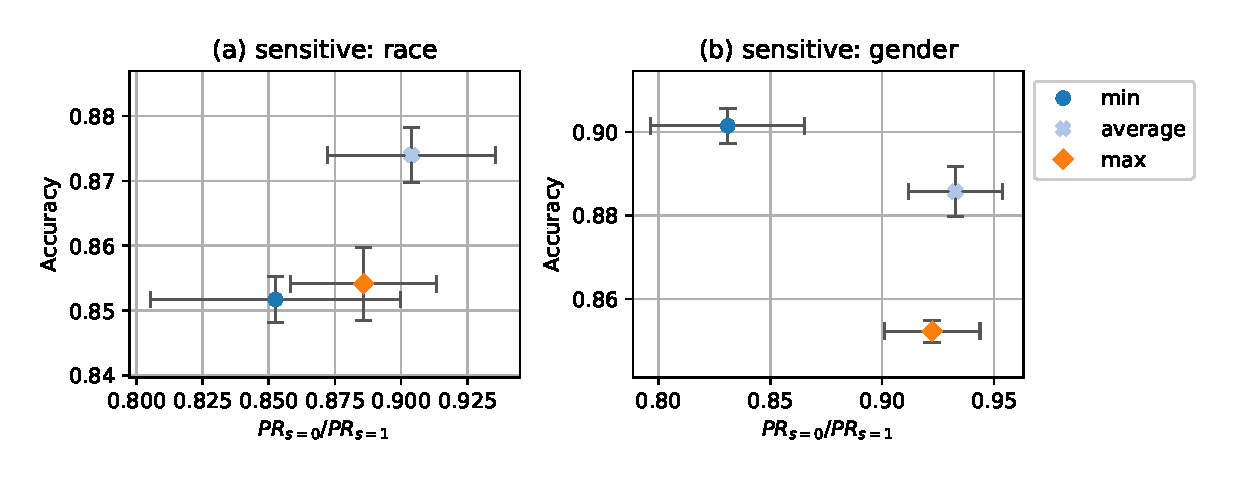
\includegraphics[width=0.98\columnwidth]{./figures/adult_tar_choice.eps}}
    \caption{Accuracy and fairness (demographic parity) for various target choices.
      (a): Adult dataset using race as the sensitive attribute;
      (b): Adult dataset using gender.
      Centre of the cross is the mean; height and width of the box encode half of standard derivation of accuracy and disparate impact.
    }%
    \label{fig:tar}
  \end{center}
  % \vspace*{-0.8cm}
% \caption{Accuracy and fairness for various targets.  w.r.t. accuracy and width of the box encodes standard derivation w.r.t. fairness criterion}
\end{figure}%
%
Following \citet{zafar2017fairnessconstraints} we evaluate demographic parity on the Adult dataset.
Table~\ref{tab:dempar} shows the accuracy and fairness for several algorithms.
In the table, and in the following, we use $\mathit{PR}_{s=i}$ to denote
the observed rate of positive predictions per demographic group $P (\hat{y} = 1 | s =i)$.
Thus, $\mathit{PR}_{s=0} / \mathit{PR}_{s=1}$ is a measure for demographic parity,
where a completely fair model would attain a value of $1.0$.
This measure for demographic parity is also called ``disparate impact''
(see e.g.~\citet{feldman2015certifying,zafar2017fairnesstreatment}).
%
As the results in Table~\ref{tab:dempar} show, FairGP and FairLR are clearly fairer than the baseline GP and LR\@.
We use the mean ($\mathit{PR}_t^{avg}$) for the target acceptance rate.
The difference between fair models and unconstrained models is not as large with \emph{race} as the sensitive attribute,
as the unconstrained models are already quite fair there.
The results of FairGP are characterised by high fairness and high accuracy.
FairLR achieves similar results to FairGP, but with generally slightly lower accuracy but better fairness.
We used the two step procedure of \citet{DonOneBenShaetal18}
to verify that we cannot achieve the same fairness result with just parameter search on LR\@.

In Fig.~\ref{fig:tar}, we investigate which choice of target ($\mathit{PR}_t^{avg}$, $\mathit{PR}_t^{min}$ or $\mathit{PR}_t^{max}$)
gives the best result.
We use $\mathit{PR}_t^{avg}$ for all following experiments as this is the fairest choice (cf. Section~\ref{sec:dp}).
The Fig.\ref{fig:tar}(a) shows results from Adult dataset with \emph{race} as sensitive attribute
where we have $\mathit{PR}_t^{min}=0.156$, $\mathit{PR}_t^{max}=0.267$ and $\mathit{PR}_t^{avg} =0.211$.
$\mathit{PR}_t^{avg}$ performs best in term of the trade-off.%equal (for \emph{race} as sensitive attribute)
%or better (for \emph{gender}) compared with the two other possibilities.
% The variant that uses $s$ for training and prediction (``use $s$'') performs significantly better here.
%\emph{ZafarAccuracy} can achieve good fairness results at the cost of accuracy.
\begin{figure}[t]
  \centering
  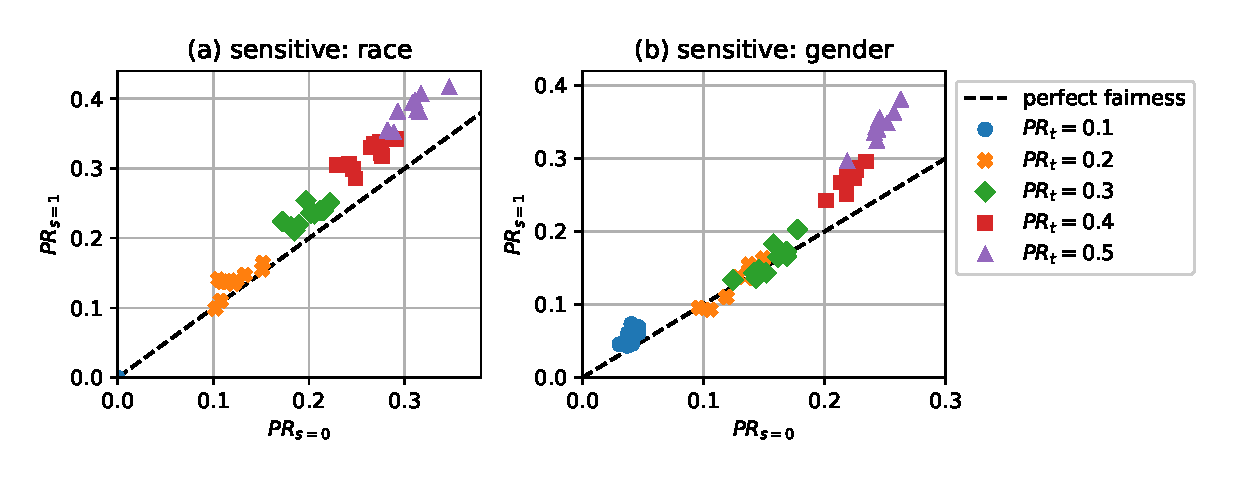
\includegraphics[width=0.98\textwidth]{./figures/adult_parity_scatter_pr_pr.eps}
  \caption{
    Predictions with different target acceptance rates (demographic parity) for 10 repeats.
    (a): $\mathit{PR}_{s=0}$ vs $\mathit{PR}_{s=1}$ using race as the sensitive attribute;
    (b): $\mathit{PR}_{s=0}$ vs $\mathit{PR}_{s=1}$ using gender.
  }%
  \label{fig:adult_parity_scatter_pr_pr}
\end{figure}
\begin{figure}[t]
  \centering
  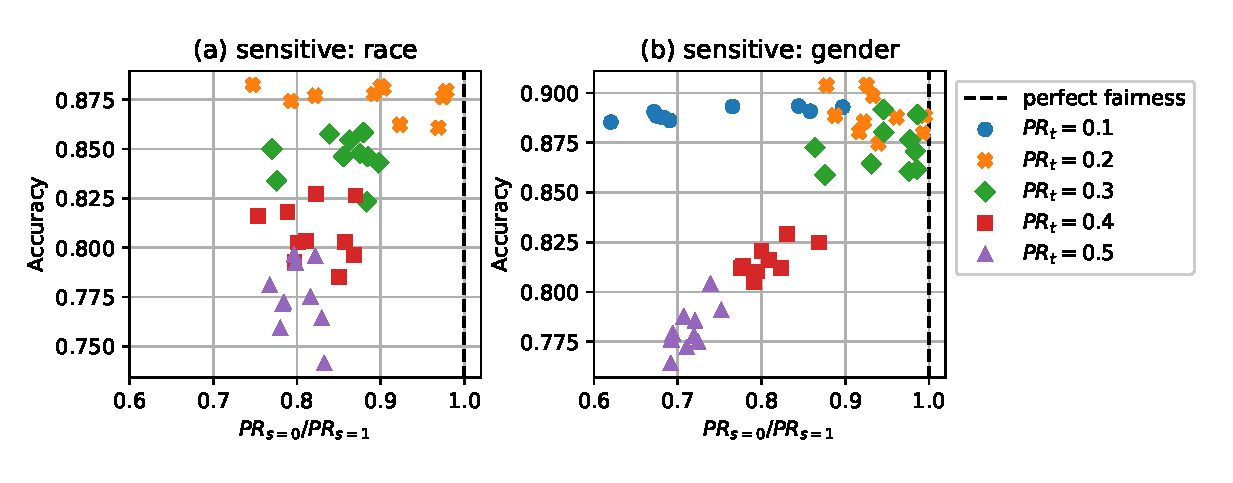
\includegraphics[width=0.98\textwidth]{./figures/adult_parity_scatter_acc.eps}
  \caption{
    Predictions with different target acceptance rates (demographic parity) for 10 repeats.
    (a): disparate impact vs accuracy on Adult dataset using race as the sensitive attribute;
    (b): disparate impact vs accuracy using gender.
  }%
  \label{fig:adult_parity_scatter_acc}
\end{figure}

Fig.~\ref{fig:adult_parity_scatter_pr_pr}(a) and (b) show runs of FairLR
where we explicitly set a target acceptance rate, $\mathit{PR}_t := P(\bar{y}=1)$,
instead of taking the mean $\mathit{PR}_t^{avg}$.
A perfect targeting mechanism would produce a diagonal.
%The data points are not exactly on the diagonal
The plot shows that setting the target rate has the expected effect on the observed acceptance rate.
This tuning of the target rate is the unique aspect of the approach.
This would be very difficult to achieve with existing fairness methods;
a new constraint would have to be added.
The achieved positive rate is, however, usually a bit lower than the targeted rate (e.g.\ around 0.15 for the target 0.2).
This is due to using imperfect classifiers;
if TPR and TNR differ from 1,
the overall positive rate is affected (see e.g.\ \citet{forman2005counting} for discussion of this).

Fig.~\ref{fig:adult_parity_scatter_acc}(a) and (b) show the same data
as Fig.~\ref{fig:adult_parity_scatter_pr_pr} but with different axes.
It can be seen from this Fig.~\ref{fig:adult_parity_scatter_acc}(a) and (b)
that the fairness-accuracy trade-off is usually best
when the target rate is close to the average of the positive rates in the dataset
(which is around 0.2 for both sensitive attribute).
%that the target acceptance rate can be used to \emph{control} the trade-off between accuracy and fairness.
%the target acceptance rate is not a trade-off parameter between accuracy and fairness.
%In this specific case, changing the target rate barely affects fairness and
%it only affects the accuracy because target acceptance rates that are different from the base acceptance rate
%necessarily lead to ``miss-classifications''.
% More details are given in the Appendix (Table~\ref{tab:adult-parity} and Table~\ref{tab:adult-tar}).

\subsection{Results for Equality of Opportunity on ProPublica dataset.}\label{sssec:eqoppresults}
% \noindent\textbf{Results for Equality of Opportunity on ProPublica dataset.}
%
For equality of opportunity,
we again follow \citet{zafar2017fairnesstreatment} and evaluate the algorithm on the ProPublica dataset.
As we did for demographic parity,
we define a measure of equality of opportunity via the ratio of the true positive rates (TPRs) within the demographic groups.
We use $\mathit{TPR}_{s=i}$ to denote the observed TPR in group $i$: $P(\hat{y}=1|y=1, s=i)$,
and $\mathit{TNR}_{s=i}$ for the observed true negative rate (TNR) in the same manner.
The measure is then given by $\mathit{TPR}_{s=0} / \mathit{TPR}_{s=1}$.
A perfectly fair algorithm would achieve $1.0$ on the measure.
\begin{figure*}[t]
  \centering
  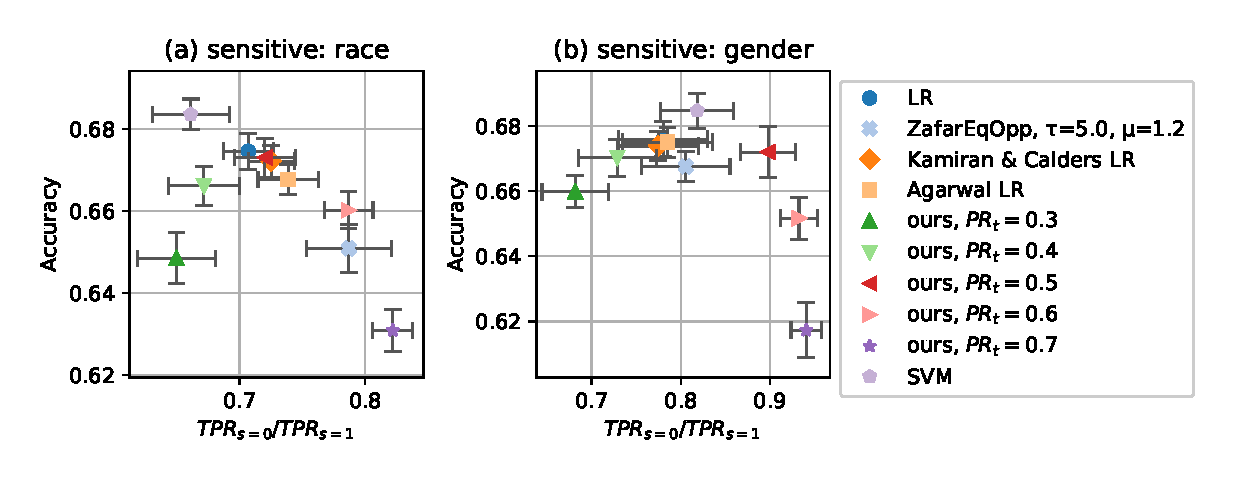
\includegraphics[width=0.98\textwidth]{./figures/propublica_opp_box_with_agarwal.eps}
%   \includegraphics[width=0.45\textwidth]{propublica-recidivism_race_opp_box.eps}
%   \includegraphics[width=0.45\textwidth]{propublica-recidivism_sex_opp_box.eps}
  \caption{Accuracy and fairness (with respect to \emph{equality of opportunity}) for various methods on ProPublica dataset.
    \textbf{(a)}: using race as the sensitive attribute; \textbf{(b)}: using gender.
    A completely fair model would achieve a value of 1.0 in the x-axis.
    %The best value for the TPR ratio is $1.0$.
    See Fig.~\ref{fig:propublica_opp_scatter_tpr}(a) and (b) on how these choices of PR setting translate to
    $\mathit{TPR}_{s=0}$ vs $\mathit{TPR}_{s=1}$. %and TPR vs TNR.
  }%
  \label{fig:propublica_opp_box}
\end{figure*}
\begin{figure*}[!ht]
  \centering
  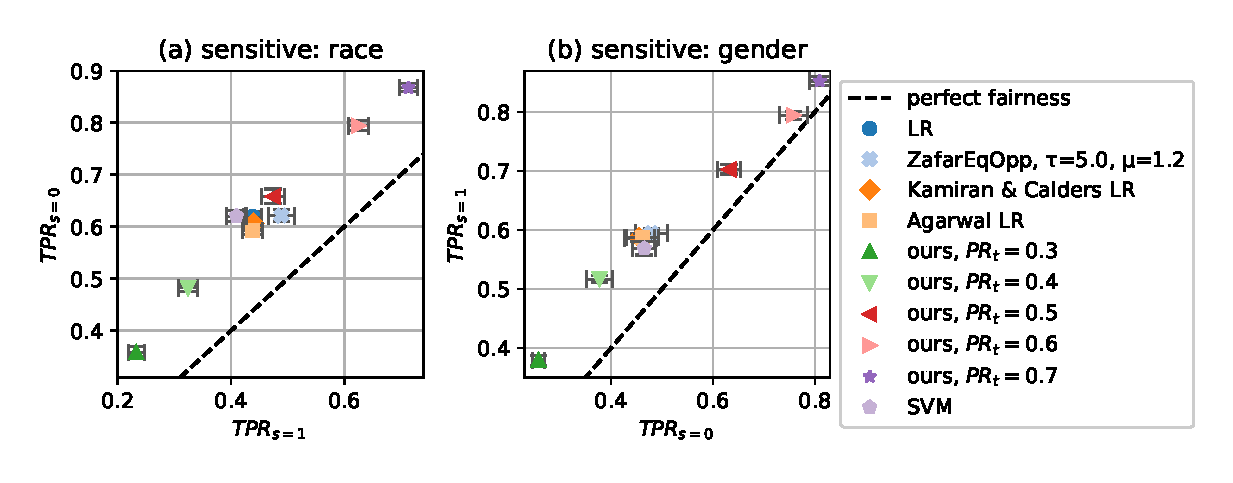
\includegraphics[width=0.98\textwidth]{./figures/propublica_opp_scatter_tpr.eps}
  \caption{%
    Fairness measure $\mathit{TPR}_{s=0}$ vs $\mathit{TPR}_{s=1}$ (\emph{equality of opportunity}) for different target PRs ($\mathit{PR}_t$).
    (a): on dataset ProPublica recidivism using race as the sensitive attribute;
    (b): using gender.
  }%
  \label{fig:propublica_opp_scatter_tpr}
\end{figure*}

The results of 10 runs are shown in Fig.~\ref{fig:propublica_opp_box} and Fig.~\ref{fig:propublica_opp_scatter_tpr}.
Fig.~\ref{fig:propublica_opp_box}(a) and (b) show the accuracy-fairness trade-off;
Fig.~\ref{fig:propublica_opp_scatter_tpr}(a) and (b) show the achieved TPRs.
In the accuracy-fairness plot, varying $\mathit{PR}_t$ is shown to produce an inverted U-shape:
Higher $\mathit{PR}_t$ still leads to improved fairness, but at a high cost in terms of accuracy.

The latter two plots make clear that the TPR ratio does not tell the whole story:
the realisation of the fairness constraint can differ substantially.
By setting different target PRs for our method, we can affect TPRs as well,
where higher $\mathit{PR}_t$ leads to higher TPR,
stemming from the fact that making more positive predictions increases the chance of making correct positive predictions.
Fig.~\ref{fig:propublica_opp_scatter_tpr} shows that our method can span a wide range of possible TPR values.
Tuning these hidden aspects of fairness is the strength of our method.

\section{Discussion and conclusion}
Fairness is fundamentally not a challenge of algorithms alone, but very much a sociological challenge.
%
A lot of proposals have emerged recently for defining and obtaining fairness in machine learning-based decision making systems. 
%
% A vast amount
The vast majority of academic work has focused on two categories of definitions: statistical (group) notions of fairness and individual notions of fairness (see~\cite{verma2018fairness} for at least twenty different notions of fairness).
%
Statistical notions are easy to verify but do not provide protections to individuals. 
%
Individual notions do give individual protections but need strong assumptions, such as the availability of an agreed-upon similarity metric, which can be difficult in practice.
%
We acknowledge that a proper solution to algorithmic fairness cannot rely on statistics alone.
%
Nevertheless, these statistical fairness definitions can be helpful in understanding the problem and working towards solutions.
%
To facilitate this, at every step, the trade-offs that are present should be made very clear
and long-term effects have to be considered as well~\citep{liu2018delayed,kallus2018residual}.
% For example, it can be the case that false positives and false negatives are not equally costly,
% in which case a closer inspection of

Here, we have developed a machine learning framework which allows us to learn from an implicit balanced dataset,
thus satisfying the two most popular notions of fairness \citep{verma2018fairness}, demographic parity
(also known as \emph{avoiding disparate treatment}) and equality of opportunity (or \emph{avoiding disparate mistreatment}).
Additionally, we indicate how to extend the framework to cover conditional demographic parity as well.
The framework allows us to set a \emph{target rate} to control how the fairness constraint is realised.
%set a \emph{target rate} for a variety of fairness notions, including demographic parity and equality of opportunity. %equalized odds, 
For example, we can set the target positive rate for demographic parity to be $0.6$ for different groups.
Depending on the application, it can be important to specify
whether non-discrimination ought to be achieved by more positive predictions or more negative predictions.
%
This capability is unique to our approach and can be used as an intuitive mechanism to control the realisation of fairness.
Our framework is general and will be applicable for sensitive variables with binary and multi-level values.
The current work focuses on a single binary sensitive variable. %, but can be extended
Future work could extend our tuning approach to other fairness concepts like the closely related predictive parity group fairness~\citep{chouldechova2017fair}
or individual fairness~\citep{dwork2012fairness}.

% Reviewer: Here: I would like to ask the authors to clarify
% whether the proposed method can be used to enforce or to address other notions of fairness; among many I mention:
% conditional statistical parity, disparate treatment, disparate mistreatment ,
% or others based on predicted risk scores and actual outcome known as 'calibration'. A discussion of this would be useful.

%Enforcement of demographic parity (also known as avoiding disparate treatment) corresponds to affirmative action
%which is in many respects not an ideal solution.
%Equality of opportunity (or avoiding disparate mistreatment) seeks to be an improvement
%because the true label is taken into account as well.
%Calibration is rarely advocated, but is another possibility.
%See~\cite{verma2018fairness} for a comparison of fairness definitions.

%\section*{Conflict of Interest Statement}
%%All financial, commercial or other relationships that might be perceived by the academic community as representing a potential conflict of interest must be disclosed. If no such relationship exists, authors will be asked to confirm the following statement: 
%% The authors declare that the research was conducted in the absence of any commercial or financial relationships that could be construed as a potential conflict of interest.

%The authors declare that this study received funding from Nvidia Corporation and Amazon.com, Inc. The funder was not involved in the study design, collection, analysis, interpretation of data, the writing of this article or the decision to submit it for publication.

% \section*{Author Contributions}

% The Author Contributions section is mandatory for all articles, including articles by sole authors. If an appropriate statement is not provided on submission, a standard one will be inserted during the production process. The Author Contributions statement must describe the contributions of individual authors referred to by their initials and, in doing so, all authors agree to be accountable for the content of the work. Please see  \href{http://home.frontiersin.org/about/author-guidelines#AuthorandContributors}{here} for full authorship criteria.

% \section*{Funding}
% N.\ Quadrianto is supported by the UK EPSRC project EP/P03442X/1

\section*{Acknowledgements}
Supported by the UK EPSRC project EP/P03442X/1 `EthicalML: Injecting Ethical and Legal Constraints into Machine Learning Models'
and the Russian Academic Excellence Project `5--100'.
% This manuscript has been released as a pre-print at arXiv \citep{kehrenberg2018tuning}.
We gratefully acknowledge NVIDIA for GPU donations, and Amazon for AWS Cloud Credits.
We thank Chao Chen and Songzhu Zheng for their inspiration of our main proof.

% \section*{Supplemental Data}
%  \href{http://home.frontiersin.org/about/author-guidelines#SupplementaryMaterial}{Supplementary Material} should be uploaded separately on submission, if there are Supplementary Figures, please include the caption in the same file as the figure. LaTeX Supplementary Material templates can be found in the Frontiers LaTeX folder.

% \section*{Data Availability Statement}
% The datasets [GENERATED/ANALYZED] for this study can be found in the [NAME OF REPOSITORY] [LINK].
% Please see the availability of data guidelines for more information, at https://www.frontiersin.org/about/author-guidelines#AvailabilityofData

% \bibliographystyle{frontiersinSCNS_ENG_HUMS} % for Science, Engineering and Humanities and Social Sciences articles, for Humanities and Social Sciences articles please include page numbers in the in-text citations
%\bibliographystyle{frontiersinHLTH&FPHY} % for Health, Physics and Mathematics articles
% \bibliography{references.bib}

%%% Make sure to upload the bib file along with the tex file and PDF
%%% Please see the test.bib file for some examples of references

%%% Please be aware that for original research articles we only permit a combined number of 15 figures and tables, one figure with multiple subfigures will count as only one figure.
%%% Use this if adding the figures directly in the mansucript, if so, please remember to also upload the files when submitting your article
%%% There is no need for adding the file termination, as long as you indicate where the file is saved. In the examples below the files (logo1.eps and logos.eps) are in the Frontiers LaTeX folder
%%% If using *.tif files convert them to .jpg or .png
%%%  NB logo1.eps is required in the path in order to correctly compile front page header %%%

% \begin{figure*}[ht]
%   \centering
%   \includegraphics[width=0.45\textwidth]{adult_race_tar.eps}
%   \includegraphics[width=0.45\textwidth]{adult_sex_tar.eps}
%   \caption{
%     Accuracy and fairness (with respect to \emph{demographic parity})
%     in the prediction for our model with different target acceptance rates.
%     Top: Adult dataset using race as the sensitive attribute; Bottom: Adult dataset using gender.
%   }
%   \label{fig:diacc_demo}
% \end{figure*}
% \begin{figure*}[!ht]
% \centering
% \includegraphics[width=0.85\textwidth]{./figures/adult_parity_box.pdf}
% %   \includegraphics[width=0.495\textwidth]{adult_race_demo_box.eps}
% %   \includegraphics[width=0.495\textwidth]{adult_sex_demo_box.eps}
%   \caption{
%     Accuracy and fairness (with respect to \emph{demographic parity}) for various methods.
%     Center of the box is the mean, height of the box encodes the standard deviation w.r.t. accuracy
%     and width of the box encodes the standard deviation w.r.t. DIbinary.
%     The best value of DIbinary is 1.
%     (a): Adult dataset using race as the sensitive attribute; (b): Adult dataset using gender.
%   }
%   \label{fig:adult_parity_box}
% \end{figure*}

% \begin{figure*}[t]
%   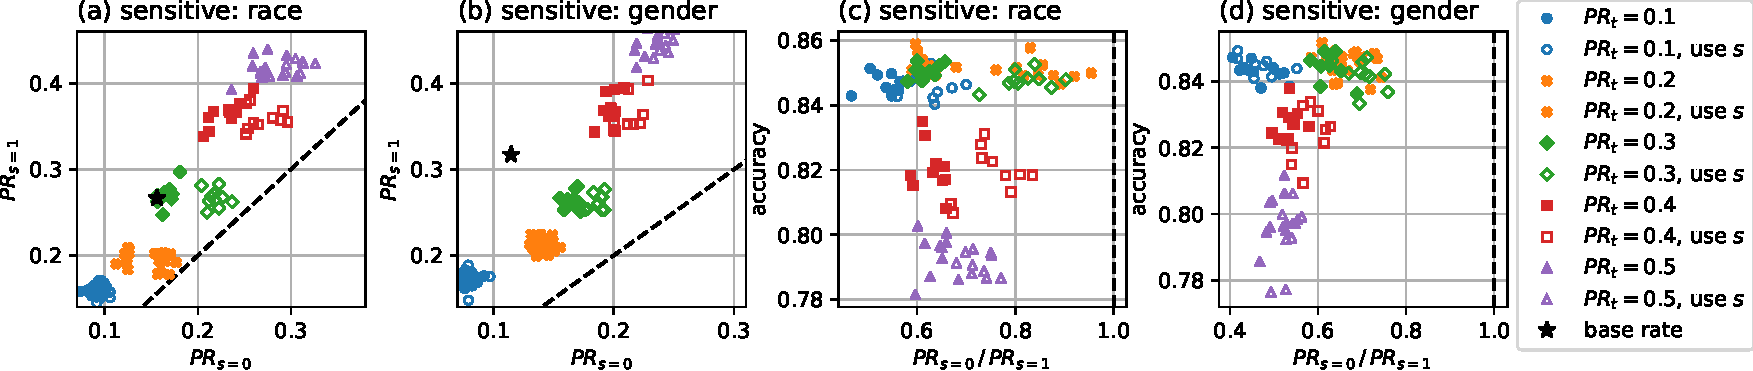
\includegraphics[width=0.98\textwidth]{./figures/adult_parity_scatter.pdf}
%   \caption{%
%     Predictions with different target acceptance rates (demographic parity) on Adult dataset.
%     \textbf{(a)} and \textbf{(b)}: $\mathit{PR}_{s=0}$ vs $\mathit{PR}_{s=1}$.
%     \textbf{(c)} and \textbf{(d)}: $\mathit{PR}_{s=0} / \mathit{PR}_{s=1}$ vs accuracy.
%     Left column:  using race as the sensitive attribute;
%     Right column:  using gender.
%     The \emph{base rate} indicates the positive rates of the training data.
%     ``use s'' indicates that $s$ was appended to the input features.
%   }%
%   \label{fig:adult_parity_scatter}
% \end{figure*}
% \begin{figure*}[t]
%   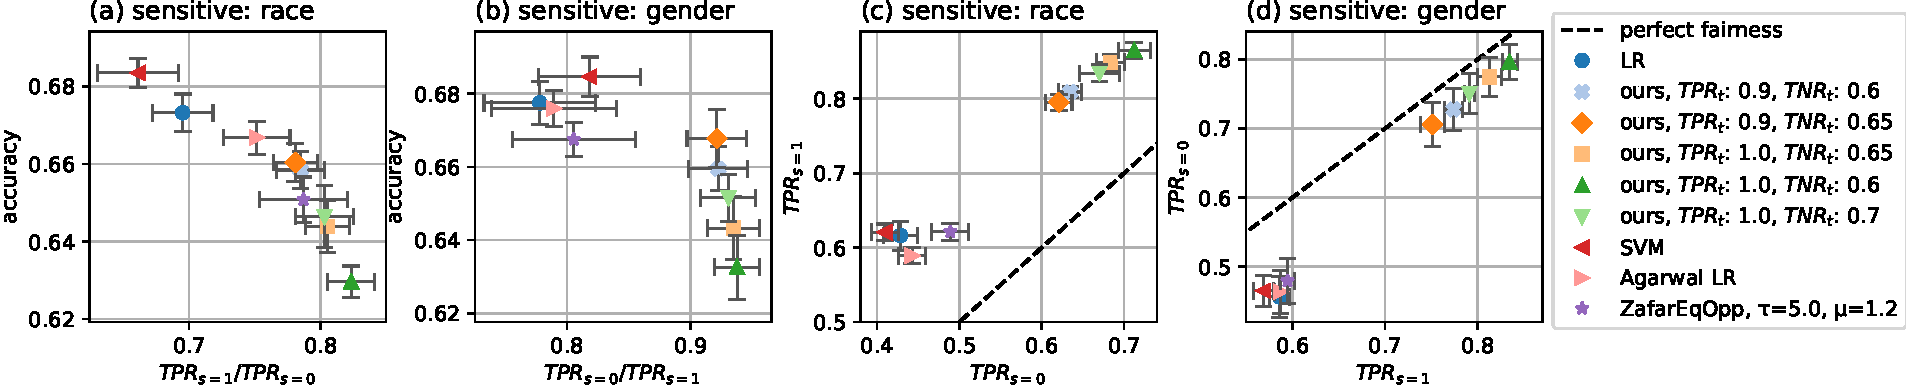
\includegraphics[width=0.98\textwidth]{./figures/eo_together.pdf}
%   \caption{%
%     Predictions with different target true positive rates ($\mathit{TPR}_t$; equality of opportunity) on ProPublica dataset.
%     Our results were obtained with the Logistic Regression model.
%     \textbf{(a)} and \textbf{(b)}: $\mathit{TPR}_{s=0} / \mathit{TPR}_{s=1}$ vs accuracy.
%     \textbf{(c)} and \textbf{(d)}: $\mathit{TPR}_{s=0}$ vs $\mathit{TPR}_{s=1}$.
%     Left column:  using race as the sensitive attribute;
%     Right column:  using gender.
%     $s$ is \emph{not} used as an input feature.
%   }%
%   \label{fig:propublica_opp_scatter}
% \end{figure*}
%
%

% \begin{figure*}[!ht]
%   \centering
%   \includegraphics[width=0.45\textwidth]{propublica-recidivism_raceTPRset_odd_tpr.eps}
%   \includegraphics[width=0.45\textwidth]{propublica-recidivism_sexTPRset_odd_tpr.eps}
%   \caption{
%     $\mathit{TPR}_{s=0}$ and $\mathit{TPR}_{s=1}$  (with respect to \emph{equality of opportunity}) for various methods.
%     Top: ProPublica recidivism using race as the sensitive attribute; Bottom: ProPublica recidivism using gender.
%   }
%   \label{fig:odds_tpr_opp}
% \end{figure*}
% \begin{figure*}[!ht]
%   \centering
%   \includegraphics[width=0.45\textwidth]{propublica-recidivism_race_opp_box_tpr_tnr.eps}
%   \includegraphics[width=0.45\textwidth]{propublica-recidivism_sex_opp_box_tpr_tnr.eps}
%   \caption{
%     TPR and TNR (with respect to \emph{equality of opportunity}) for various methods.
%     Top: ProPublica recidivism using race as the sensitive attribute; Bottom: ProPublica recidivism using gender.
%   }
%   \label{fig:odds_tpr_tnr_opp}
% \end{figure*}

% Figures \ref{fig:odds_tpr_opp} and \ref{fig:odds_opp} show the results from experiments
% where the target TPR rate was set manually
% instead of being estimated from training and evaluating on the pre-validation and pre-training set.
% \begin{figure*}[!ht]
%   \centering
%   \includegraphics[width=0.98\textwidth]{./figures/propublica_opp_scatter_tnr.pdf}
%   \caption{%
%     $\mathit{TPR}$ vs $\mathit{TNR}$ for different target TPRs ($\mathit{TPR}_t$).
%     (a): on dataset ProPublica recidivism using race as the sensitive attribute;
%     (b): using gender.
%   }%
%   \label{fig:propublica_opp_scatter_tnr}
% \end{figure*}

%%% If you are submitting a figure with subfigures please combine these into one image file with part labels integrated.
%%% If you don't add the figures in the LaTeX files, please upload them when submitting the article.
%%% Frontiers will add the figures at the end of the provisional pdf automatically
%%% The use of LaTeX coding to draw Diagrams/Figures/Structures should be avoided. They should be external callouts including graphics.
% \clearpage
\section{Appendix}
\subsection{Proof of Theorem 1}
Let $\eta(x,s)=P(y=1|x,s)$ be the distribution of the training data.
% todo: specify the tysbakov condition explicitly
Let $\bar{\eta}(x, s)=m_s\cdot\eta(x,s)+b_s$, where
% problem: the definition of m_s and b_s is different to before
\begin{align}
  m_s&=P(\bar{y}=1|y=1,s)-P(\bar{y}=1|y=0,s)\nonumber\\
  &=1-P(\bar{y}=0|y=1,s)-P(\bar{y}=1|y=0,s)\\
  b_s&=P(\bar{y}=1|y=0,s)
\end{align}
So, $\bar{\eta}(x, s)=P(\bar{y}=1|x, s)$.
Let $y$ denote the \emph{hard} labels for $\eta$: $y=\mathbb{I}\left[\eta>\tfrac{1}{2}\right]$ and $\bar{y}$ be the hard labels for $\bar{\eta}$: $\bar{y}=\mathbb{I}\left[\bar{\eta}>\tfrac{1}{2}\right]$.

\begin{theorem}\label{th:tsybakov}
  The probability that $y$ and $\bar{y}$ disagree ($y\neq\bar{y}$) for any input $x$ in the dataset is given by:
  \begin{align}
    P(y\neq\bar{y}|s)=P\left(\left|\eta(x,s) - \tfrac{1}{2}\right| < t_s\right)
  \end{align}
  where
  \begin{align}
    t_s = \left|\frac{m_s+2b_s-1}{2m_s}\right|~.\label{eq:def-ts2}
  \end{align}
\end{theorem}
\begin{proof}
  The decision boundary that lets us recover the true labels is at $\tfrac{1}{2}$ (independent of $s$).
  So, for the shifted distribution, $\bar{\eta}$, this threshold to get the true labels would be at $\tfrac{1}{2}\cdot m_s + b_s$ (it depends on $s$ now).
  If we however use the decision boundary of $\tfrac{1}{2}$ for $\bar{\eta}$, to make our predictions, $\bar{y}$, then this prediction will sometimes not correspond to the true label, $y\neq\bar{y}$. When does this happen?

  Let $d_s$ be the new decision boundary: $d_s=\tfrac{1}{2}\cdot m_s + b_s$. There are two possibilities to consider here:
  either $\tfrac{1}{2}<d_s$ or $\tfrac{1}{2}>d_s$ (for $d_s=\tfrac{1}{2}$, the decision boundaries are the same and nothing has to be shown).
  The problem, $y\neq\bar{y}$, appears then exactly when the value of $\bar{\eta}$ is between the two boundaries:
  \begin{align}
    \text{if}~d_s>\tfrac{1}{2}\text{:}\quad d_s>\bar{\eta}(x, s)>\tfrac{1}{2} \\
    \text{if}~d_s<\tfrac{1}{2}\text{:}\quad d_s<\bar{\eta}(x, s)<\tfrac{1}{2}
  \end{align}
  Expressing this in terms of $\eta$ and simplifying leads to
  (if $m_s$ is negative, then the two cases are swapped, but we still get both inequalities):
  \begin{align}
    \text{if}~d_s>\tfrac{1}{2}\text{:}\quad\frac{1}{2}>\eta(x,s)>\frac{1-2b_s}{2m_s} \\
    \text{if}~d_s<\tfrac{1}{2}\text{:}\quad\frac{1}{2}<\eta(x,s)<\frac{1-2b_s}{2m_s}
  \end{align}
  This can be summarized as
  \begin{align}
    \left|\eta(x,s)-\frac{1}{2}\right|<\left|\frac{1}{2}-\frac{1-2b_s}{2m_s}\right|~.
  \end{align}
  Let $t_s$ denote the term on the right side of this inequality (i.e. the ``threshold'' that determines whether $y=\bar{y}$ or not). Then
  \begin{align}
    t_s=\left|\frac{1}{2} -\frac{1-2b_s}{2m_s}\right|=\left|\frac{m_s+2b_s-1}{2m_s}\right|~.
  \end{align}
  So, we have: $\left|\eta(x, s) - \frac{1}{2}\right| < t_s =\left|\tfrac{m_s+2b_s-1}{2m_s}\right|$.
  This leads directly to the statement we wanted to prove:
  \begin{align}
    P(y\neq\bar{y}|s)=P\left(\left|\eta(x, s)-\frac{1}{2}\right| <t_s\right)~.
  \end{align}
\end{proof}

\subsection{Finding minimal $t_s$}
We express $t_s$ in terms of $\mathit{PR}_b^s$ and $\mathit{PR}_t$.
\begin{align}
  t_s = \begin{cases}
    \frac{1}{2}\frac{\mathit{PR}_b^s - \mathit{PR}_t}{\mathit{PR}_t} &\text{if }\mathit{PR}_t>\mathit{PR}_b^j\\
    \frac{1}{2}\frac{\mathit{PR}_t - \mathit{PR}_b^s}{1 - \mathit{PR}_t} &\text{otherwise.}
  \end{cases}\label{eq:ts-pr2}
\end{align}
Without loss of generality, we assume $\mathit{PR}_b^0<\mathit{PR}_b^1$.
As mentioned in the main text, 
$\mathit{PR}_t$ should be between $\mathit{PR}_b^0$ and $\mathit{PR}_b^1$ to minimize both $t_s$.
If that is the case, then we get
\begin{align}
  t_{s=0} &= \frac{1}{2}\frac{\mathit{PR}_t - \mathit{PR}_b^0}{1 - \mathit{PR}_t}\\
  t_{s=1} &= \frac{1}{2}\frac{\mathit{PR}_b^1 - \mathit{PR}_t}{\mathit{PR}_t}~.
\end{align}
If we further assume $\mathit{PR}_b^1<\tfrac{1}{2}$,
then we also have $\mathit{PR}_t<\tfrac{1}{2}$ and thus $\mathit{PR}_t<1-\mathit{PR}_t$.
This implies that the denominator of $t_{s=1}$ is smaller and that, in turn, $t_{s=1}$ grows faster.
This faster growth means that when minimizing $t_{s=0} + t_{s=1}$, we have to concentrate on $t_{s=1}$.
The minimum is then such that $t_{s=1}$ is 0, i.e.\ $\mathit{PR}_t=\mathit{PR}_b^1$.

\subsection{Proof of Theorem 2}
We are given a dataset $\mathcal{D} = {\{(x_i, y_i)\}}_i$,
where the $x_i$ are vectors of features and the $y_i$ the corresponding labels.
We refer to the tuples $(x, y)$ as the \emph{samples} of the dataset.
The number of samples is $N = |\mathcal{D}|$.

We assume binary labels ($y\in \{0, 1\}$) and thus can form the (disjoint) subsets $\mathcal{\mathcal{Y}}^0$ and $\mathcal{Y}^1$ with
\begin{align}
  \mathcal{Y}^j = \{(x, y)\in \mathcal{D}|y = j\}\quad\text{with } j\in\{0, 1\}~.
\end{align}
Furthermore, we associate each sample with a classification $\hat{y}\in \{0, 1\}$.
The task of making the classification $\hat{y}=0$ or $\hat{y}=1$ can be understood as putting each sample from $\mathcal{D}$
into one of two sets: $\mathcal{C}^0$ and $\mathcal{C}^1$,
such that $\mathcal{C}^0\cup\mathcal{C}^1 = \mathcal{D}$ and $\mathcal{C}^0\cap\mathcal{C}^1 = \emptyset$.

We refer to the set $\mathcal{A} = (\mathcal{C}^0\cap\mathcal{Y}^0) \cup (\mathcal{C}^1\cap\mathcal{Y}^1)$
as the set of correct (or \textbf{a}ccurate) predictions.
The \emph{accuracy} is given by $\mathit{acc} = N^{-1}\cdot\left|\mathcal{A}\right|$.
From the definition it is clear that $0\leq\mathit{acc} \leq 1$.

\begin{definition}
  \begin{align}
    r_a := \frac{\left|\mathcal{Y}^1\right|}{|\mathcal{D}|} = \frac{\left|\mathcal{Y}^1\right|}{N}
  \end{align}
  is called the \emph{acceptance rate} of the dataset $\mathcal{D}$.
\end{definition}

\begin{definition}
  \begin{align}
    \hat{r}_a = \frac{\left|\mathcal{C}^1\right|}{|\mathcal{D}|} = \frac{\left|\mathcal{C}^1\right|}{N}
  \end{align}
  is called the \emph{target rate} of the predictions.
\end{definition}

\begin{theorem}
  For a dataset with the acceptance rate $r_a$ and corresponding predictions with a target rate of $\hat{r}_a$,
  the accuracy is limited by
  \begin{align}
    \mathit{acc} \leq 1 - \left| \hat{r}_a -r_a \right|~.
  \end{align}
\end{theorem}
\begin{proof}
  We first note that by multiplying by $N$, the inequality becomes
  \begin{align}
    |\mathcal{A}| \leq N - \left| |\mathcal{C}^1| -|\mathcal{Y}^1| \right|~.
  \end{align}
  We will choose the predictions $\hat{y}$ that achieve the highest possible accuracy (largest possible $\mathcal{A}$)
  and show that this can never exceed $1 - \left| \hat{r}_a -r_a \right|$.
  As the set $\mathcal{Y}^1$ contains all samples that correspond to $y=1$,
  we try to take as many samples from $\mathcal{Y}^1$ for $\mathcal{C}^1$ as possible.
  Likewise, we take as many indices as possible from $\mathcal{Y}^0$ for $\mathcal{C}^0$.

  % We consider three cases: $\left|\mathcal{C}^1\right| = \left|\mathcal{Y}^1\right|$, $\left|\mathcal{C}^1\right| > \left|\mathcal{Y}^1\right|$
  % and $\left|\mathcal{C}^1\right| < \left|\mathcal{Y}^1\right|$.
  We consider three cases: $\hat{r}_a = r_a$, $\hat{r}_a < r_a$ and $\hat{r}_a > r_a$.
  The first case is trivial;
  we have $\left|\mathcal{C}^1\right| = \left|\mathcal{Y}^1\right|$ and thus
  are able to set $\mathcal{C}^1 = \mathcal{Y}^1$, $\mathcal{C}^0 = \mathcal{Y}^0$ and achieve perfect accuracy ($\mathit{acc} \leq 1$).

  For $\hat{r}_a < r_a$, we have $\left|\mathcal{C}^1\right| < \left|\mathcal{Y}^1\right|$
  and thus have more samples available with $y = 1$ than we would optimally need to select for $\mathcal{C}^1$.
  There are two terms to consider that make up the definition of $\mathcal{A}$:
  $\mathcal{C}^0 \cap \mathcal{Y}^0$ and $\mathcal{C}^1\cap \mathcal{Y}^1$.
  The intersection of these two terms is empty because $\mathcal{C}^0\cap \mathcal{C}^1 = \emptyset$.
  Thus,
  \begin{align}
    \left|\mathcal{A}\right| &= \left|(\mathcal{C}^0\cap\mathcal{Y}^0) \cup (\mathcal{C}^1\cap\mathcal{Y}^1)\right|
    = \left|(\mathcal{C}^0\cap\mathcal{Y}^0)\right| + \left|(\mathcal{C}^1\cap\mathcal{Y}^1)\right|~.
  \end{align}
  Selecting samples from $\mathcal{Y}^1$ for $\mathcal{C}^0$ will only \emph{decrease} the first term,
  so for maximum accuracy, it is fine to take as many samples from $\mathcal{Y}^1$ for $\mathcal{C}^1$.
  Taking all available samples from $\mathcal{Y}^1$ such that $\mathcal{C}^1 \supset \mathcal{Y}^1$,
  there is still space left in $\mathcal{C}^1$ which we will have to fill with samples with $y=0$.
  Thus, we have $\mathcal{C}^1\cap \mathcal{Y}^1 = \mathcal{Y}^1$.
  For $\mathcal{C}^0$, we have enough $y=0$ such that
  $\mathcal{C}^0\subset \mathcal{Y}^0$ and $\mathcal{C}^0\cap \mathcal{Y}^0 = \mathcal{C}^0$.
  This is the largest we can make these intersections.
  Putting everything together:
  \begin{align}
    \left|\mathcal{A}^\mathit{optimal}\right|
    &= \left|(\mathcal{C}^0\cap\mathcal{Y}^0)\right| + \left|(\mathcal{C}^1\cap\mathcal{Y}^1)\right|
     = \left|\mathcal{C}^0\right| + \left|\mathcal{Y}^1\right|\nonumber\\
    &= N - \left|\mathcal{C}^1\right| + \left|\mathcal{Y}^1\right|
     = N - \left(\left|\mathcal{C}^1\right| - \left|\mathcal{Y}^1\right|\right)~.
  \end{align}

  For $\hat{r}_a > r_a$, the roles of $\mathcal{C}^0$ and $\mathcal{C}^1$ are reversed
  and thus, the signs in the equation are inverted:
  \begin{align}
    \left|\mathcal{A}^\mathit{optimal}\right| = N  - (\left|\mathcal{Y}^1\right| - \left|\mathcal{C}^1\right|)~.
  \end{align}
  This proves the claim.
\end{proof}
\begin{corollary}
  Given a dataset that consists of two subsets $\mathcal{S}_0$
  and $\mathcal{S}_1$ ($\mathcal{D} = \mathcal{S}_0 \cup \mathcal{S}_1$)
  where $p$ is the ratio of $|\mathcal{S}_0|$ to $|\mathcal{D}|$
  and given corresponding acceptance rates $r^0_a$ and $r^1_a$
  and predictions with target rates $\hat{r}^0_a$ and $\hat{r}^1_a$,
  the accuracy is limited by
  \begin{align}
    \mathit{acc} \leq 1 - p\cdot\left| \hat{r}^0_a -r^0_a \right| - (1-p)\cdot\left| \hat{r}^1_a -r^1_a \right|~.
  \end{align}
\end{corollary}
\begin{figure}[t]
  \centering
  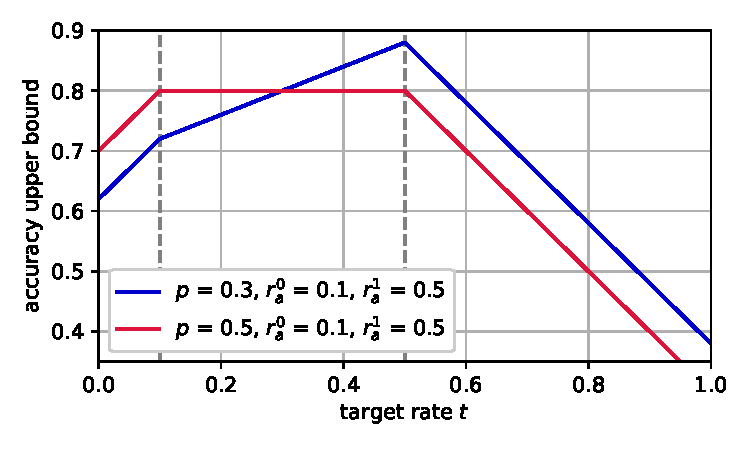
\includegraphics[width=0.5\textwidth]{./figures/plot.pdf}
  \caption{Achievable accuracy for different target values.}%
  \label{fig:accvstarget}
\end{figure}
\begin{example}
  We consider the case where $S_0$
  (which could for example be all data points for female individuals) makes up 30\% of the dataset; so $p = 0.3$.
  Further, we say that for $S_0$ we have an acceptance rate of 10\% ($r^0_a = 0.1$)
  and for $S_1$, 50\% ($r^1_a = 0.5$).
  If we then set both target rates to the same value $t$ ($\hat{r}^0_a=\hat{r}^1_a=t$), with $t = 0.3$,
  then the highest accuracy that can be achieved is $0.8$ or 80\%.

  Fig~\ref{fig:accvstarget} shows the achievable accuracy for different values of $t$ in blue:
  We can see that we can achieve the highest accuracy for $t=r^1_a=0.5$, namely 88\%.
  The plot in orange shows the achievable accuracy for $p=0.5$, i.e., when the two subsets have the same size.
  In this case, all target rates between $r^0_a$ and $r^1_a$ give equal results, namely 80\%.
\end{example}

\subsection{Illustration of restrictions on PR}
\begin{figure}[t]
  \centering
  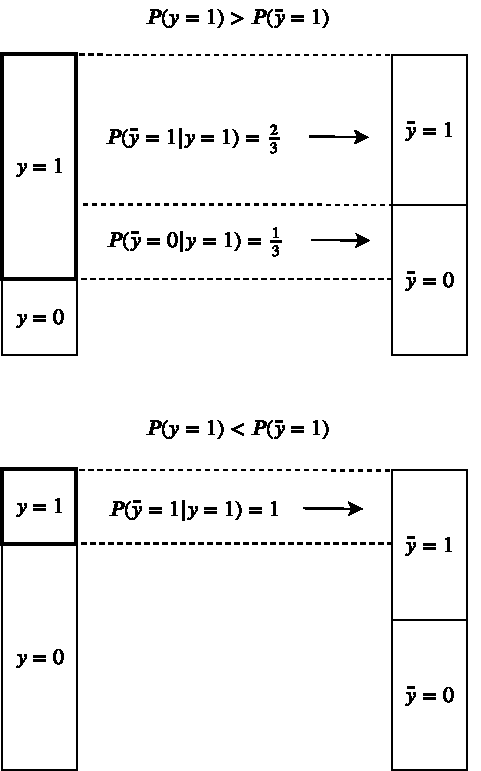
\includegraphics[width=0.3\textwidth]{figures/label_shift.pdf}
  \caption{%
    Illustration of demographic parity with target labels.
    In the situation in the upper part, $P(\bar{y}=1|y=1)$ cannot be set to 1,
    because there are more samples with $y=1$ than there are $\bar{y}=1$.
    In the situation in the lower part, $P(\bar{y}=1|y=1)$ can be set to 1.
  }%
  \label{fig:shift}
\end{figure}%
We start by setting a target rate $r_t$:
\begin{align}
  P(\bar{y}=1|s=0) \overset{!}{=} r_t \quad\text{and}\quad P(\bar{y}=1|s=1) \overset{!}{=} r_t
\end{align}

This leads us to the following constraint for $s\prime\in\{0, 1\}$:
\begin{align}
  r_t &= P(\bar{y}=1|s=s\prime)\nonumber\\
  &= \sum\limits_y P(\bar{y}=1|y,s=s\prime) P(y|s=s\prime)
\end{align}

For $P(y|s=s\prime)$ we will put in the value at which we want our constraint to hold.
We denote $P(y=1|s=j)$ as the base rate $r_b^j$ which we estimate from the training set.
Plugging this in, we are left with
\begin{align}
  r_t = \,\,&P(\bar{y}=1|y=0,s=0) \cdot (1-r_b^0) \nonumber\\
  +\, &P(\bar{y}=1|y=1,s=0) \cdot r_b^0 \\
  r_t = \,\,&P(\bar{y}=1|y=0,s=1) \cdot (1-r_b^1)\nonumber\\
  +\, &P(\bar{y}=1|y=1,s=1) \cdot r_b^1~.
\end{align}
This is a system of linear equations with two equations and four free variables.
There is thus still considerable freedom in how we want our constraint to be realized.
The freedom that we have here concerns how strongly the accuracy will be affected.

If we set $P(\bar{y}=1|y=1,s)$ to 0.5,
then we express the fact that a train label of 1 only implies a target label of 1 in 50\% of the cases.
In order to minimize the effect on accuracy,
we make $P(\bar{y}=1|y=1,s)$ as high as possible and $P(\bar{y}=1|y=0,s)$ as low as possible.

We solve for $P(\bar{y}=1|y=0,s=j)$:
\begin{align}
  &P(\bar{y}=1|y=0,s=j)\nonumber\\
  =\,\, &\frac{r_b^j}{1-r_b^j} \left(\frac{r_t}{r_b^j} - P(\bar{y}=1|y=1,s=j)\right)~.
\end{align}
However, we can set $P(\bar{y}=1|y=0,s=j)$ to 0
only if that does not imply $P(\bar{y}=1|y=1,s=j)$ will be greater than 1.
This would happen if $\nicefrac{r_t}{r_b^j}$ were greater than 1.

Figure~\ref{fig:shift} illustrates this.
In the upper part of the figure we have $\nicefrac{r_t}{r_b^j}$ less than 1.
In this case

% \section{Supplementary Tables and Figures}

% For more information on Supplementary Material and for details on the different file types accepted, please see \href{http://home.frontiersin.org/about/author-guidelines#SupplementaryMaterial}{the Supplementary Material section} of the Author Guidelines.

% \subsection{Figures}

%%% There is no need for adding the file termination, as long as you indicate where the file is saved. In the examples below the files (logo1.eps and logos.eps) are in the Frontiers LaTeX folder
%%% If using *.tif files convert them to .jpg or .png
%%%  NB logo1.eps is required in the path in order to correctly compile front page header %%%


% \end{document}

\chapter{Paper 2: Null-sampling for Interpretable and Fair Representations}\label{ch:paper2}
% \documentclass[runningheads]{llncs}
% \pdfoutput=1
% \usepackage[utf8]{inputenc}
% \usepackage{graphicx}
% \usepackage{comment}
% \usepackage{biblatex}
% \usepackage{placeins}
% \usepackage{amsmath,amssymb,amsfonts,bm} % define this before the line numbering.
% \usepackage{color}
% \usepackage{booktabs}

% \usepackage{import}
% \usepackage{appendix}
% \usepackage[caption=false]{subfig}
% \usepackage{mathtools}
% \usepackage{wrapfig}
% \usepackage{hyperref}

% \def\ci{\perp\!\!\!\perp}
% \newcommand*\diff{\mathop{}\!\mathrm{d}}
% \def\httilde{\mbox{\tt\raisebox{-.5ex}{\symbol{126}}}}

% \addbibresource{references.bib}

% \begin{document}

% \pagestyle{headings}
% \mainmatter
% \def\ECCVSubNumber{5488}  % Insert your submission number here

% \title{Null-sampling for Interpretable \\and Fair Representations} % Replace with your title

% \titlerunning{Null-sampling for Interpretable and Fair Representations}
% \author{Thomas Kehrenberg \and
% Myles Bartlett \and
% Oliver Thomas \and \\
% Novi Quadrianto}
% \authorrunning{T. Kehrenberg et al.}
% \institute{Predictive Analytics Lab (PAL), University of Sussex, Brighton, UK
% \email{\{t.kehrenberg,m.bartlett,ot44,n.quadrianto\}@sussex.ac.uk}}
% \maketitle

\textsc{Authors}:\\
Thomas Kehrenberg$^1$, Myles Bartlett$^1$, Oliver Thomas$^1$, and Novi Quadrianto$^1$ \\
\textsc{Affiliations}:\\
$^1$ Predictive Analytics Lab (PAL), University of Sussex, Brighton, UK\\
\textsc{Conference}:\;\;\textit{European Conference on Computer Vision} (ECCV), 2020 \\
% \textsc{DOI}:\;\;10.3389/frai.2020.00033
\textsc{Note}:\;\;The appendix has been included as section~\ref{sec:nifr-appendix}.

% 70-150 words
\section{Abstract}
\noindent
% Training data often contains spurious correlations not reflected in the real world where a trained model will be deployed.
% Consequently, computer vision and machine learning systems can become over-reliant on these correlations for classifications.
% Instead of basing their output on those features which are semantically meaningful, the output can be based on these unintended relationships.
% This is undesirable for many reasons, among them limited generalisation and uncontrolled bias.
We propose to learn invariant representations, in the data domain, to achieve interpretability in algorithmic fairness. 
Invariance implies a selectivity for high level, relevant correlations w.r.t.\ class label annotations, and a robustness to irrelevant correlations with protected characteristics such as race or gender. 
We introduce a non-trivial setup in which the training set exhibits a strong bias such that class label annotations are irrelevant and spurious correlations cannot be distinguished.
To address this problem, we introduce an adversarially trained model with a \emph{null-sampling} procedure to produce invariant representations in the data domain.
To enable disentanglement, a partially-labelled \emph{representative} set is used.
By placing the representations into the data domain, the changes made by the model are easily examinable by human auditors.
We show the effectiveness of our method on both image and tabular datasets: Coloured MNIST, the CelebA and the Adult dataset.%
% At the same time, it is important the people be able to trust the outputs of machine learning systems 
% To address this problem, we propose dividing training into a straightforward and general two-step procedure.
% In this framework, the model is first trained to produce invariant representations from an unlabelled pre-training set, in which there exists minimal spurious correlations.
% In the second step a classifier is trained on the encoding generated for the biased training set.
% We first demonstrate the viability of our  No Shortcuts in Neural Network (NoSiNN) framework with a AutoEncoder model before showing how its drawbacks can be ameliorated through the use of an Invertible architecture.
% Experiments with face images, coloured digits, and census data show promising results in decorrelating the spurious and non-spurious semantic features.

\section{Introduction}
% We need to stare start with something with more punch
%r rather than just a f matter-of-fact statement
%Fair representations are a means of removing potentially sensitive information from training data
%in order to avoid wrongly relying on the sensitive information for classification.

Without due consideration for the data collection process, machine learning algorithms can exacerbate biases, or even introduce new ones if proper control is not exerted over their learning \cite{holstein2019improving}. 
While most of these issues can be solved by
% While efforts should be made to
controlling and curating data collection in a fairness-conscious fashion, 
% aiming to eliminate algorithmic bias during the early stages of the pipeline, 
doing so is not always an option, such as when working with historical data.
Efforts to address this problem algorithmically have been centred on developing statistical definitions of fairness and learning models that satisfy these definitions.
One popular definition of fairness used to guide the training of fair classifiers, for example, is \emph{demographic parity}, stating that positive outcome rates should be equalised (or \emph{invariant}) across protected groups.

In the typical setup, we have an input $\bm{x}$, a sensitive attribute $s$ that represents some non-admissible information like gender
and a class label $y$ which is the prediction target.
The idea of fair \emph{representation} learning \cite{ZemWuSwePitetal13}\cite{edwardsstorkey}\cite{madras2018learning}
is then to transform the input $\bm{x}$ to a representation $\bm{z}$ which is invariant to $s$.
Thus, learning from $\bm{z}$ will not introduce a forbidden dependence on $s$.
% $\bm{z}$ can then be used to learn a predictor
% In fair representation learning \cite{ZemWuSwePitetal13}\cite{edwardsstorkey}\cite{madras2018learning}, the goal is then to find a representation $\bm{z}$ that is invariant to $s$.
A good fair representation is one that preserves most of the information from $\bm{x}$ while satisfying the aforementioned constraints.
% While fair \emph{representations} are by no means the only method of achieving this goal, approaches that explicitly depend on the target label \cite{kamiran2012data} are restrictive in that they do not readily admit transfer to unseen tasks, and are bound by the requirement of having $s$ and $y$ labels be present together.

As unlabelled data is much more freely available than labelled data, it is of interest to learn the representation in an unsupervised manner.
This will allow us to draw on a much more diverse pool of data to learn from.
% ; this is particularly pertinent for fair representation learning as unlabelled data affords us a much more diverse pool of data to learn from.
%To this end, \cite{locatello2019fairness} recently made the connection from disentangled representations to fair representations:
%a model for disentanglement trained without knowledge of the sensitive attribute $s$
%nevertheless appears to improve fairness measures with respect to $s$.
%However, as pointed out by \cite{locatello2019challenging},
%some supervision or inductive bias is needed in order to recognise a well-disentangled representation.
While annotations for $y$ are often hard to come by (and often noisy \cite{KehCheQua18}),
annotations for the sensitive attribute $s$ are usually less so, as $s$ can often be obtained from demographic information provided by census data.
We thus consider the setting where the representation is learned from data
that is only labelled with $s$ and not $y$.
This is in contrast to most other representation learning methods.
% We thus consider the setting where data labelled with $s$ (partially labelled data) is available for learning the fair representation.
% Furthermore, we assume the existence of a set with $s$ labels
% whose distribution matches the deployment setting
We call the set used to learn the representation the \emph{representative} set,
because its distribution is meant to match the distribution of the deployment setting
(and is thus representative).
% We call this set the \emph{representative} set and its distribution is meant to match the distribution of the deployment setting.

Once we have learnt the mapping from $\bm{x}$ to $\bm{z}$,
we can transform the \emph{training} set which, in contrast to the representative set, has the $y$ labels (and $s$ labels).
In order to make our method more widely applicable,
we consider an \emph{aggravated fairness problem}
% we allow the case
in which the training set contains a strong spurious correlation between $s$ and $y$,
which makes it impossible to learn from it a representation which is invariant to $s$ but not invariant to $y$.
Non-invariance to $y$ is important in order to be able to predict $y$.
The training set thus does \emph{not} match the deployment setting,
thereby rendering the representative set essential for learning the right invariance.
% We also tackle the related problem of learning from biased data, specifically cases in which the training set (with $y$ labels) contains a strong spurious correlation between $s$ and $y$, and thus does not match the deployment setting.
From hereon, we will use the terms \emph{spurious} and \emph{sensitive} interchangeably, depending on the context, to refer to an attribute of the data we seek invariance to.
% This is essentially a form of strong sampling bias and is not an unrealistic complication, having been shown to plague real-world datasets \cite{kallus2018residual}.
%Classifiers trained on ImageNet for example, have been shown to be biased towards texture \cite{Geir18}. \cite{zhang2018visual} similarly examine the problem of learning from biased data, showing that pre-trained models can exploit biases in the data by learning patterns semantically unrelated to the target, an issue that can be difficult to identify when the bias pervades both the training and test sets.
We can draw a connection between learning in the presence of spurious correlations and what \cite{kallus2018residual} call \emph{residual unfairness}.
Consider the Stop, Question and Frisk (SQF) dataset for example:
the data was collected in New York City, but the demographics of the recorded cases do not represent the true demographics of NYC well.
The demographic attributes of the recorded individuals might correlate so strongly with the prediction target that the two are nearly indistinguishable.
This is the scenario that we are investigating: $s$ and $y$ are so closely correlated in the labelled dataset that they cannot be distinguished, but the learning of $s$ is favoured due to being the ``path of least resistance''.
The deployment setting (i.e.\ the test set) does not possess this strong correlation and thus a na\"ive approach will lead to very unfair predictions.
In this case, a disentangled representation is insufficient;
the representation needs to be explicitly invariant solely with respect to $s$.
In our approach, we make use of the (partially labelled) representative set to learn this invariant representation.

While there is a substantial body of literature devoted to the problems of fair representation-learning, exactly how the invariance in question is achieved is often overlooked. 
When critical decisions, such as who should receive bail or be released from jail, are being deferred to an automated decision making system, it is critical that people be able to trust the logic of the model underlying it, whether it be via semantic or visual explanations. 
We build on the work of \cite{QuaShaTho19} and learn a decomposition ($f^{-1}: Z_s \times Z_{\neg s} \rightarrow X$) of the \emph{data domain} ($X$) into independent subspaces \emph{invariant} to  $s$ ($Z_{\neg s}$) and \emph{indicative} of $s$ ($Z_{s}$), which lends an interpretability that is absent from most representation-learning methods.
While model interpretability has no strict definition \cite{zhang2018visual}, we follow the intuition of \cite{adel2018discovering} -- \emph{a simple relationship to something we can understand}, a definition which representations in the data domain naturally fulfil.

Whether as a result of the aforementioned sampling bias or simply because the features necessarily co-occur, it is not rare for features to correlate with one another in real-world datasets.
Lipstick and gender for example, are two attributes that we expect to be highly correlated and to enforce invariance to gender can implicitly enforce invariance to makeup.
This is arguably the desired behaviour.
However, unforeseen biases in the data may engender cases which are less justifiable.
By baking interpretability into our model (by having representations in the data domain), though we still have no better control over what is learned, we can at least diagnose such pathologies.

To render our representations interpretable, we rely on a simple transformation we call \emph{null-sampling} to map invariant representations in the data domain.
Previous approaches to fair representation learning \cite{beutel,edwardsstorkey,madras2018learning,LouSweLi15} predominantly rely upon autoencoder models to jointly minimise reconstruction loss and invariance.
We discuss first how this can be done with such a model that we refer to as cVAE (conditional VAE),
before arguing that the bijectivity of invertible neural networks (INNs)~\cite{Dinh2014} makes them better suited to this task. 
We refer to the variant of our method based on these as cFlow (conditional Flow).
INNs have several properties that make them appealing for unsupervised representation learning. 
The focus of our approach is on creating invariant representations that preserve the non-sensitive information maximally, with only knowledge of $s$ and not of the target $y$, while at the same time having the ability to easily probe what has been learnt.

% The problem of fair representations can also be viewed through a similar lens.
% A good toy model for this setup is the Coloured MNIST (cMNIST) dataset.
% In this example, the colour is a spurious variable which is very closely correlated with the prediction target in the training set but not in the deployment setting.
% An interpretable invariant representation in this case is the images uniform in colour. More details regarding the setup and synthesis of the dataset can be found in Section~\ref{ssec:cmnist}.

% As a more real-world dataset, we consider the CelebA dataset.
% We treat the CelebA dataset as it is, as the deployment setting
% and construct deliberately biased subsets of CelebA to serve as the training set.
% In our experiments we use gender as the sensitive attribute.
% Sample images can be seen in \thomas{Fig.??}.
% Attributes that are correlated with gender in the \emph{deployment setting} (like the use of lipstick) will also be removed by our method.
% We do not consider this a defect of our method and instead argue that this is the correct behaviour:
% As long as the deployment setting is sufficiently diverse, the model may make use of correlations found in there.
%wearing lipstick is a valid indicator of gender.
%\thomas{maybe don't include the previous sentence}

Our contribution is thus two-fold:
1) We propose a simple approach to generating representations 
% through use of an INN, 
that are invariant to a feature $s$, while having the benefit of interpretability that comes with being in the data domain.
We call our model \emph{NIFR} (\textbf{N}ull-sampling for \textbf{I}nterpretable and \textbf{F}air \textbf{R}epresentations).
2) We explore a setting where the labelled training set suffers from varying levels of sampling bias,
% which we expect to be common not only in fairness problems but machine learning problems more broadly,
demonstrating an approach based on transferring information from a more diverse representative set,
with guarantees of the non-spurious information being preserved.

\begin{figure*}[tb]
  \centering
  \subfloat[Original images.]{%
      \scalebox{0.3}{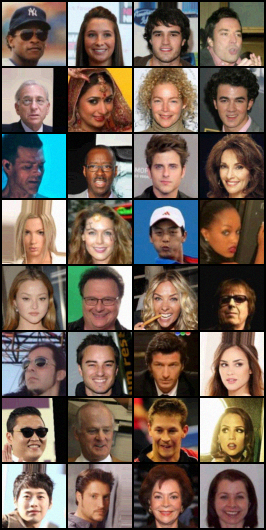
\includegraphics[width=\textwidth]{./Images/celeba/train_original_x_2.png}}%
      \label{fig:cflow_celeba_original_x}
  }
  \hfill
  \subfloat[$\bm{x}_u$ null-samples from the cFlow model.]{%
      \scalebox{0.3}{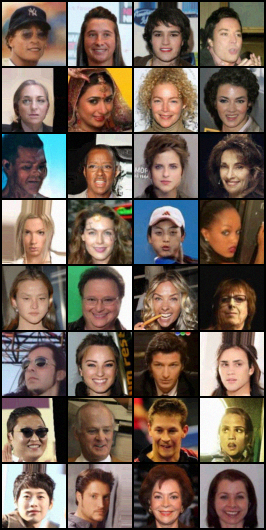
\includegraphics[width=\textwidth]{./Images/celeba/train_reconstruction_y_2.png}}%
      \label{fig:cflow_celeba_recon_y}
  }
  \hfill
  \subfloat[$\bm{x}_b$ null-samples from the cFlow model.]{%
      \scalebox{0.3}{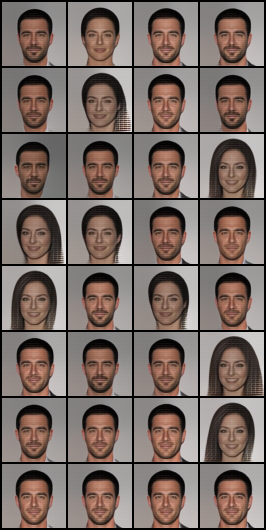
\includegraphics[width=\textwidth]{./Images/celeba/train_reconstruction_s_2.png}}%
      \label{fig:cflow_celeba_recon_s}
  }
  \caption{
    CelebA null-samples learned by our cFlow model, with gender as the sensitive attribute.
    (a) The original, untransformed samples from the CelebA dataset
    (b) Reconstructions using only information unrelated to $s$.
    (c) Reconstruction using only information related to $\neg s$.
    The model learns to disentangle gender from the non-gender related information.
    % Attributes such as \emph{makeup} and \emph{hair length} are also often modified in the process due to inherent correlations between them and the sensitive attribute, which the intepretability of our representations allows us to easily identify.
    Note that some attributes like skin tone seem to change along with gender due to the correlation between the attributes.
    This is especially visible in images (1,1) and (3,2). Only because our representations are produced in the data-domain can we easily spot such instances of entanglement.
  }%
  \label{fig:celeba_cflow}
\end{figure*}

\begin{figure*}[!htb]
    \centering
    \subfloat[Samples from the cMNIST training set, $\sigma=0$.]{%
        \scalebox{0.3}{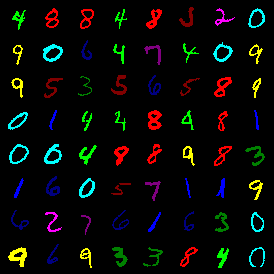
\includegraphics[width=\textwidth]{paper2/Images/cmnist/cflow_original_task_x_scale_0.png}}%
        \label{fig:cflow_cmnist_task_train}
    }
    % \hfill
    % \subfloat[Samples from the cMNIST test set with $\sigma=0.02$.]{%
    %     \scalebox{0.225}{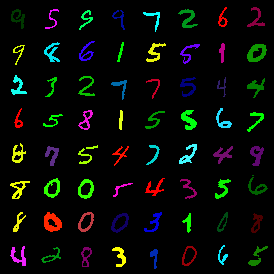
\includegraphics[width=\textwidth]{./Images/cmnist/cflow_pretrain_x.png}}%
    %     \label{fig:cflow_cmnist_pretrain}
    % }
    \hfill
    \subfloat[$x_u$ null-samples from the cFlow model.]{%
        \scalebox{0.3}{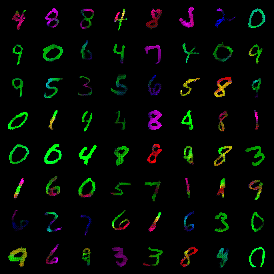
\includegraphics[width=\textwidth]{paper2/Images/cmnist/cflow_task_xy_scale_0.png}}%
        \label{fig:cflow_cmnist_y}
    }
    \hfill
    \subfloat[$x_b$ null-samples from the cFlow model.]{%
        \scalebox{0.3}{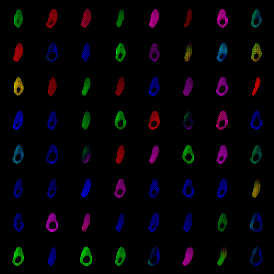
\includegraphics[width=\textwidth]{paper2/Images/cmnist/cflow_task_xs_scale_0.png}}%
        \label{fig:cflow_cmnist_s}
    }
    \caption{
        Sample images from the coloured MNIST dataset problem with $10$ predefined mean colours.
        (a): Images from the spuriously correlated subpopulation where colour is a reliable signal of the digit class-label.
        (b-c): Results of running our approach realised with cFlow on the cMNIST dataset.
        The model learns to retain the shape of the digit shape while removing the relationship with colour.
        A downstream classifier is now less prone to exploiting correlations between colour and the digit label class.
    }\label{fig:cmnist}
\end{figure*}


\section{Background}\label{sec:background}
% \noindent We frame our approach in the context of relevant literature on the interrelated problems of fair representation learning and learning representations free of spurious correlations.
% The background is far too long - we also need to touch on the interpretability literature

\subsection{Learning fair representations.}
%As we have alluded to, the goal of producing invariant representations is similar to that of producing \emph{fair} representations.
% In fairness problems, there is usually a \emph{sensitive attribute}, $s$ (for example, gender or race),
% that should not be used to make decisions.
Given a sensitive attribute $s$ (for example, gender or race) and inputs $\bm{x}$,
a fair representation $\bm{z}$ of $\bm{x}$ is then one for which $\bm{z} \perp s$ holds,
while ideally also being predictive of the class label $y$.
\citet{zemel2013learning} was the first to propose the learning of fair representations which allow for transfer to new classification tasks.
More recent methods are often based on \acfp{VAE}~\citep{kingma2013auto,louizos2016variational,edwards2016censoring,beutel2017data}.
The achieved fairness of the representation can be measured with various fairness metrics.
These measure, however, usually how fair the predictions of a classifier are
and not how fair a representation is.
% defined with respect to predictions and not representations.

% There is not one metric universally best-suited to measuring the invariance (or fairness) of representations.
The appropriate measure of fairness for a given task is domain-specific \citep{liu2018delayed}
and there is often not a universally accepted measure.
However, \emph{Demographic Parity} is the most widely used~\citep{louizos2016variational,edwards2016censoring,beutel2017data}.
Demographic Parity demands $\hat{y} \perp s$ where $\hat{y}$ refers to the predictions of the classifier.
In the context of fair representations, we measure the Demographic Parity of a downstream classifier, $f(\cdot )$, which is trained on the representation $z$, i.e.\  $f: Z \to \hat{Y}$.

A core principle of all fairness methods is the \emph{accuracy-fairness trade-off}.
As previously stated, the fair representation should be invariant to $s$ ($\to$ fairness) but still be predictive of $y$ ($\to$ accuracy).
These desiderata cannot, in general, be simultaneously satisfied if $s$ and $y$ are correlated.
% We explore this trade-off with our method as well. % DO WE?!?!?!?!?


The majority of existing methods for fair representations also make use of $y$ labels during training,
in order to ensure that $\bm{z}$ remains predictive of $y$.
This aspect can, in theory, be removed from the methods,
but then there is no guarantee that information about $y$ is preserved \citep{louizos2016variational}. 
% Existing methods designed to create fair representations can, in theory, be extended to the regime in which only the $s$, and not the $y$, labels are available. 
% However, it is not without its drawbacks as, in removing $s$, there is no guarantee that information about $y$ is preserved \cite{louizos2016variational}. 
% For this reason, $y$ is typically supplied during training and the representation encouraged to be predictive of it.

\subsection{Learning fair, transferrable representations}
% Outside of computer vision, \cite{madras2018learning} have also worked on removing a problematic spurious correlation.
In addition to producing fair representations, \citet{madras2018learning} want to ensure the representations are transferrable.
Here, an adversary is used to remove sensitive information from a representation $z$.
Auxiliary prediction and reconstruction networks, to predict class label $y$
% to ensure it remains predictive of $y$
and reconstruct the input $x$ respectively,
are trained on top of $z$, with $s$ being ancillary input to the reconstruction.
% alongside a reconstruction loss computed with respect to the output of a decoder that takes $z$ and the sensitive label $s$ as input is added. 
% This is so that $x$ can still be reconstructed from $z$, despite the removal of $s$.
%The decoder is utilised only for the purpose of maximum likelihood learning of the data distribution.
% By conditioning the decoder on the sensitive attribute, information about it can be ``off-loaded'' from the encoder such that information about $s$ need not be contained in the fair representation while still permitting the use of a reconstruction loss needed to capture non-sensitive information.
% The decoder plays a role only in the loss function.
% In contrast, we make explicit use of the decoder not only for characterising the behaviour of the model and also for evaluation.

Also related is \citet{creager2019flexibly} who employ a FactorVAE \citep{kim2018disentangling} regularised for fairness.
The idea is to learn a representation that is both disentangled and invariant to multiple sensitive attributes.
This factorisation makes the latent space easily manipulable such that the different subspaces can be freely removed and composed at test time.
Zeroing out the dimensions or replacing them with independent noise imparts invariance to the corresponding sensitive attribute.
This method closely resembles ours when we use an invertible encoder.
However, the emphasis of our approach is on interpretability, information-preservation, and coping with sampling bias - especially extreme cases where $|\, \textrm{supp}(S_{tr} \times Y_{tr}) | < |\, \textrm{supp}(S_{te} \times Y_{te}) |$.
% Namely, the invertibility of the network means we can optimise for invariance singularly without the burden of a reconstruction loss.
% While we do not explicitly consider the case of multi-attribute fairness, our method can be easily adapted for this use-case.

Attempts were made by~\citet{QuaShaTho19} prior to this work to learn fair representations in the data domain in order to make it interpretable and transferable.
In their work, the input is assumed to be additively decomposable in the feature space into a \emph{fair} and \emph{unfair} component, which together can be used by the decoder to recover the original input.
This allows us to examine representations in a human-interpretable space and confirm that the model is not learning a relationship reliant on a sensitive attribute.
Though a first step in this direction, we believe such a linear decomposition is not sufficiently expressive to fully capture the relationship between the sensitive and non-sensitive attributes.
Our approach allows for the modelling of more complex relationships.

\subsection{Learning in the presence of spurious correlations}
% As  previously  discussed,  the  goal  of  producing  fair representations is similar to the goal of producing representations invariant to spurious correlations found in the training data.
Strong spurious correlations make the task of learning a robust classifier challenging: the classifier may learn to exploit correlations unrelated to the true causal relationship between the features and label, and thereby fail to generalise to novel settings.
This problem was recently tackled by \citet{kim2019learning} who apply a penalty based on the mutual information between the feature embedding and the spurious variable. 
While the method is effective under mild biasing, we show experimentally that it is not robust to the range of settings we consider.

\citet{JacBehZemBet19} explore the vulnerability of traditional neural networks to spurious variables -- e.g., textures, in the case of ImageNet \citep{Geir18} -- and propose a INN-based solution akin to ours.
The INN's encoding is split such that one partition, $z_b$ is encouraged to be predictive of the spurious variable while the other serves as the logits for classification of the semantic label. 
Information related to the nuisance variable is ``pulled out'' of the logits as a result of maximising $\log p(s|z_n)$.
This specific approach, however, is incompatible with the settings we consider, due to its requirement that both $s$ and $y$ be available at training time.

Viewing the problem from a causal perspective, \citet{arjovsky2019invariant} develop a variant of empirical risk minimisation called invariant risk minimisation (IRM).
The goal of IRM is to train a predictor that generalises across a large set of unseen environments; because variables with spurious correlations do not represent a stable causal mechanism, the predictor learns to be invariant to them. IRM assumes that the training data is not \emph{iid} but is partitioned into distinct environments, $e \in E$. The optimal predictor is then defined as the minimiser of the sum of the empirical risk $R_e$ over this set. In contrast, we assume possession of only a single source of \emph{labelled}, albeit spuriously-correlated, data, but that we have a second source of data that is free of spurious correlations, with the benefit being that it only needs to be labelled \emph{with respect to $s$}.

% The model thereby enforces their independence.
% This is achieved with an adversarial approach, borrowing the gradient reversal technique from \cite{ganin2016domain}.
%The authors construct the coloured MNIST dataset in two steps.
%First, ten distinct colours are assigned to each digit uniquely; these colours parameterise the means of ten corresponding Gaussian distributions from which colour samples are drawn.
%The standard deviation ($\sigma$) of the Gaussian distribution controls the dispersion of the sampled colours around these means.
% To demonstrate the effectiveness of their model, \cite{kim2019learning} construct a coloured version of the MNIST dataset as follows.
% During training, colours are sampled from a Gaussian distribution (with standard deviation $\sigma$) where each digit is associated with a single fixed mean colour.
%the colours are sampled abiding by this one-to-one colour mapping;
% At test time however, a colour mean is chosen at random from the 10 mean colours used during training.
% The actual colour is sampled with the same $\sigma$ as in the training set.
%there is no such designation and colours are sampled randomly and unrestrictedly from the complete palette.
%As such, a classifier that lazily minimises its loss by treating the pixel values as a lookup table falls flat at inference owing to a shift in the distribution of the spurious variables away from that of the target's.
% We follow this approach to evaluate performance of our NoSiNN framework in a synthetic setting (see Fig. \ref{fig:cmnist} for qualitative results).

% For the training strategy of the \cite{kim2019learning} model, a neural network is trained to predict the digit class, $y$, while an adversarial network takes one of the intermediate layers as input to predict the spurious value, colour.
% The first network seeks to prevent the adversary from making correct predictions, which means discarding or obfuscating information about colour.
% For this approach to work, the adversary needs to be able to distinguish between the digit class and the colour.
% To do this, the adversary is allowed access to the sampled RGB values of the colour that it is trying to remove, and not just the mean.
% As the sampled colour varies according to the standard deviation of the Gaussian distribution, the actual colour and the digit class vary in correlation.
% As the colour becomes less descriptive of the digit class, the network learns to disentangle the two.
% This works better, the larger $\sigma$; a major limitation of the approach its failure to deal with extremely low $\sigma$ values.


% \begin{itemize}
%     \item Pix2pix and CycleGANs combined standard cGAN discriminators with L1 reconstruction loss in data domain, the latter doing so in the form of cycle consistency, allowing for translation between unpaired samples. Bidirectional GANs extend the GAN discriminator to act on the distributions in data and latent space jointly.
%     \item StarGAN \cite{choi2018stargan} provides a unified framework for performing image-to-image translation across multiple domains.
%     \item Instead of enforcing bijectivity through cycle loses, invertible neural networks are bidirectional by design
%     \item Glow achieves impressive attribute manipulations
%     \item Rather than trying to translate inputs across domains we seek to do so to a subspace which does not abide in either domain. 
    
% \end{itemize}

% \paragraph{Unsupervised approaches.} 
% There is a large literature on the unsupervised disentangling of representations; we highlight one of the more recent findings connected with our approach.
% \cite{locatello2019challenging} evidence  that the unsupervised learning of disentangled representations
% requires inductive biases on the part of both the data set and the models.
% Thus, such methods can usually only be used for a single task or kind of data.

\section{Interpretable Invariances by Null-Sampling}\label{ssec:general}
% \begin{figure}
%     \centering
%     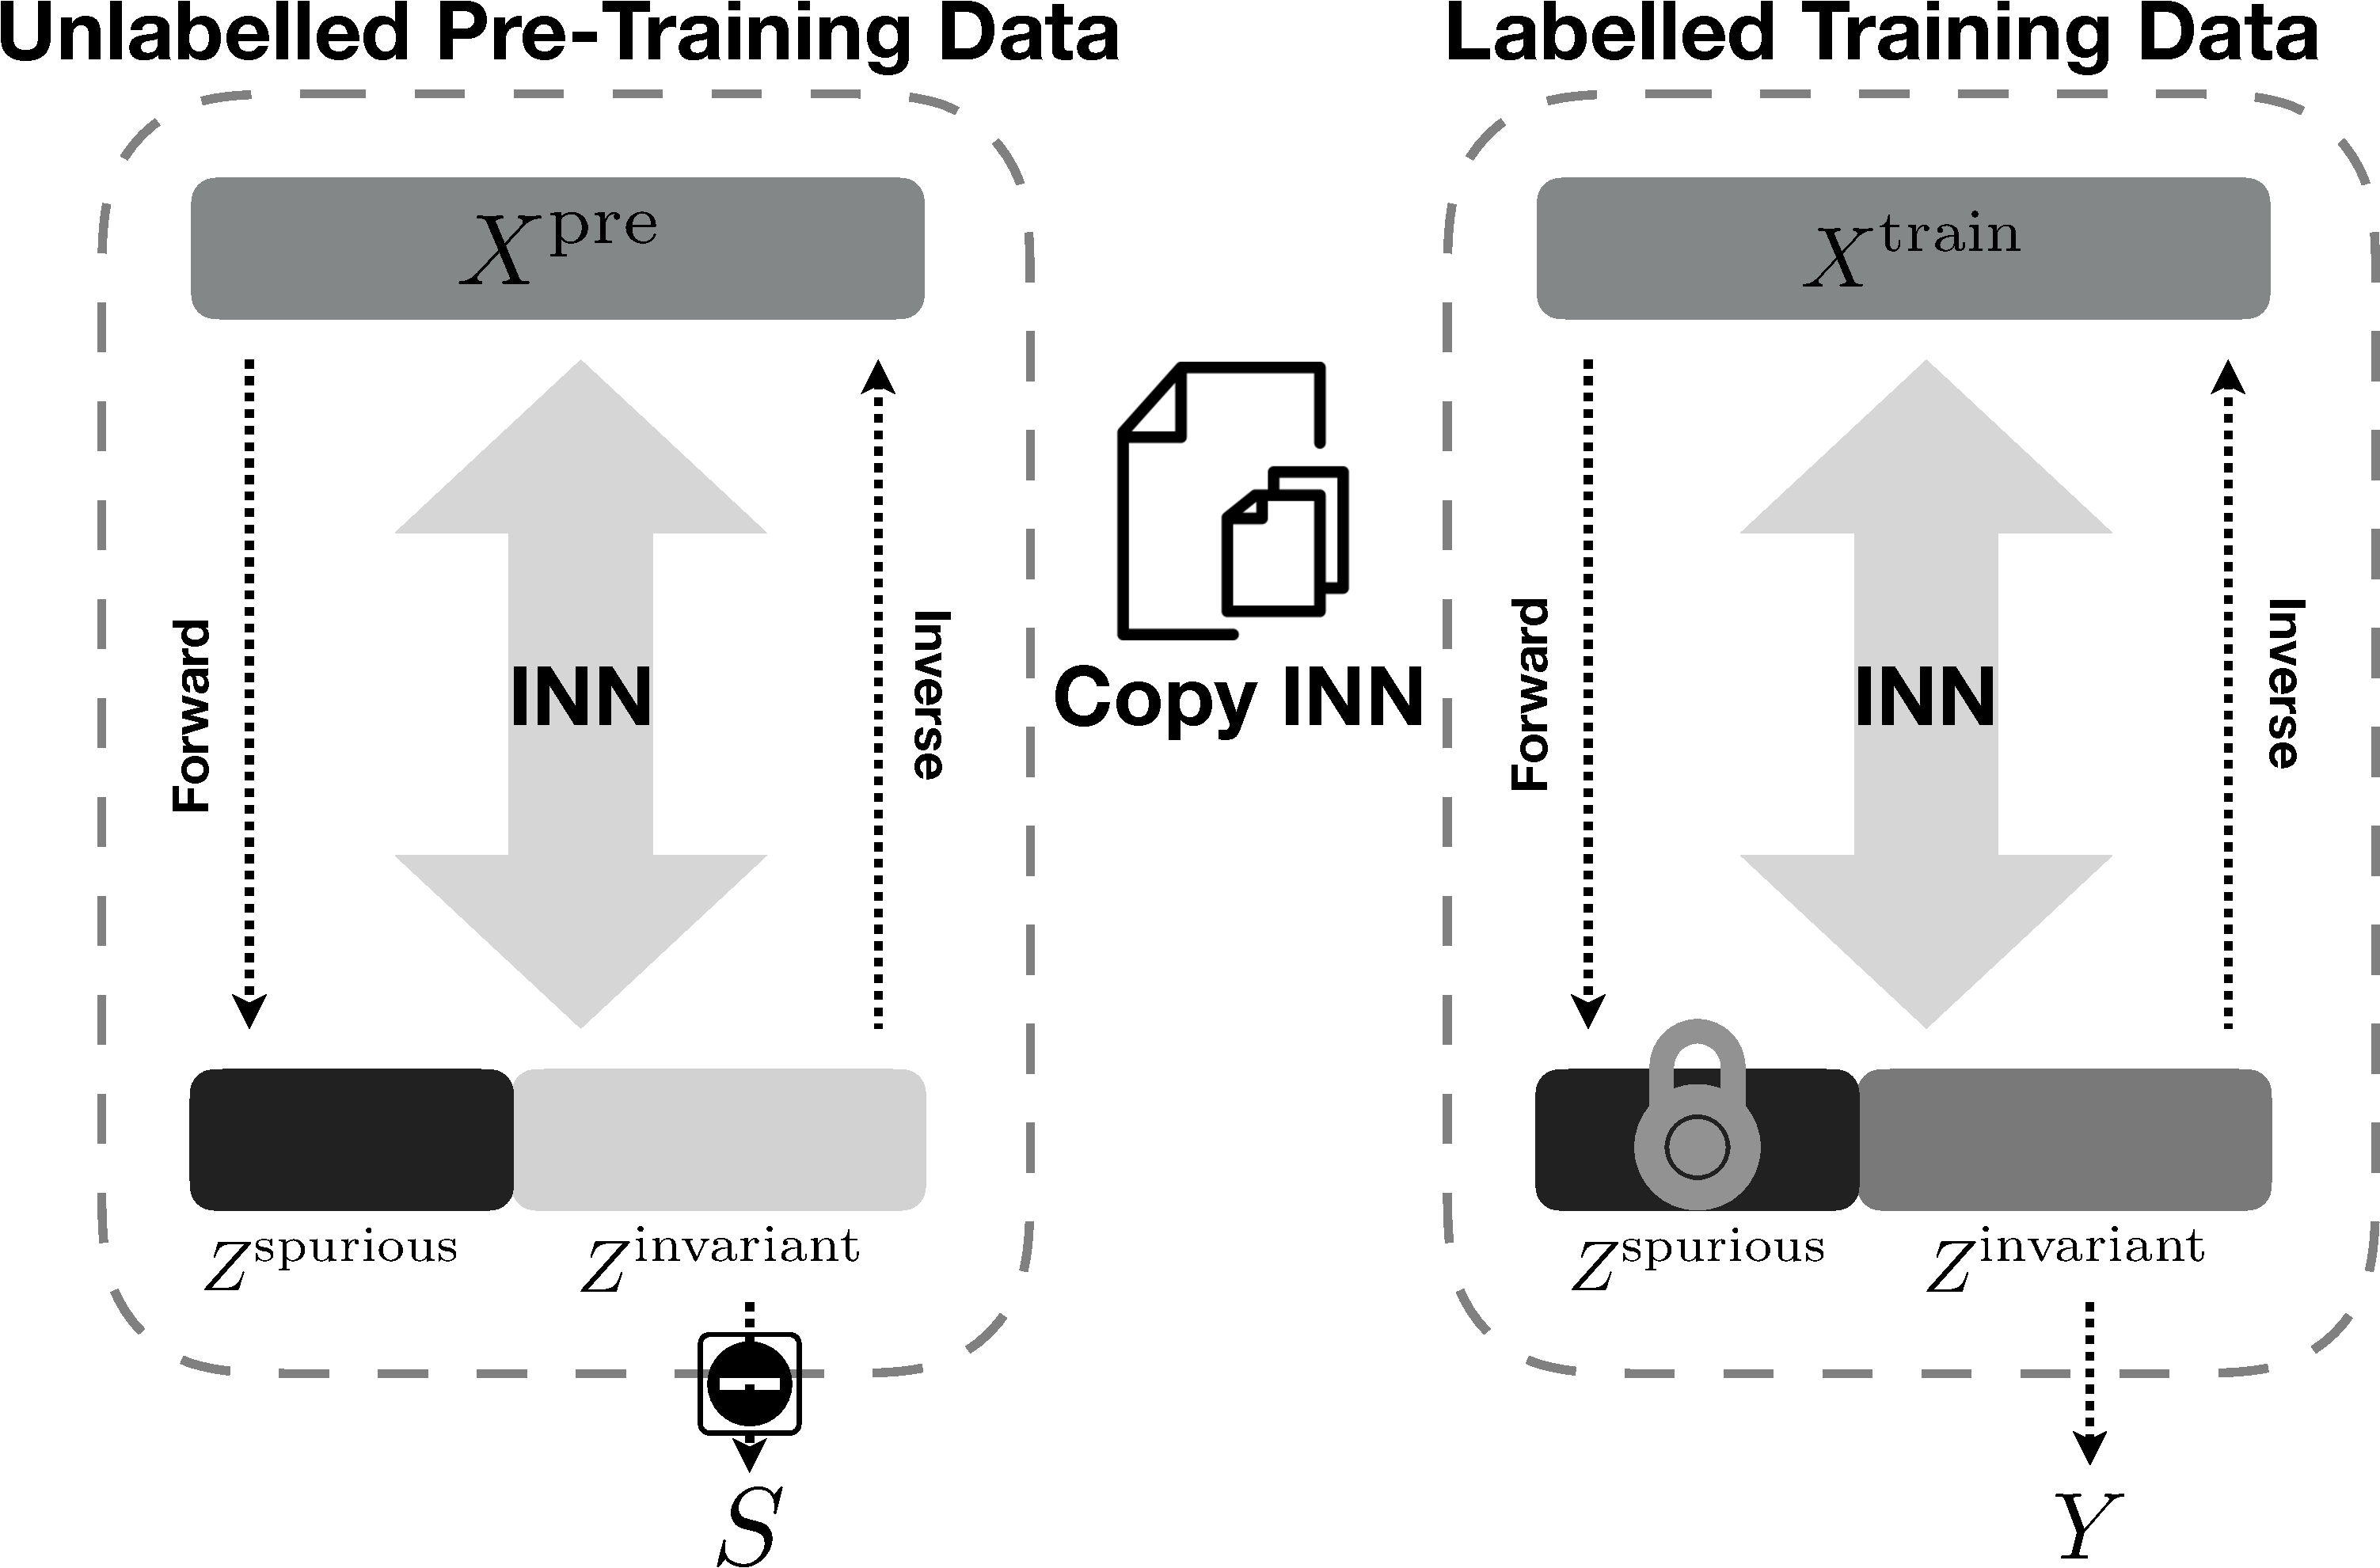
\includegraphics[width=0.4\textwidth]{./Figures/diagram.pdf}
%     \caption{Training procedure using the cFlow model for illustrative purposes.}%
%     \label{fig:training_diagram}
% \end{figure}
\begin{figure*}[tb]
    \centering
    \hfill
    \subfloat[cFlow model.]{%
        \scalebox{0.33}{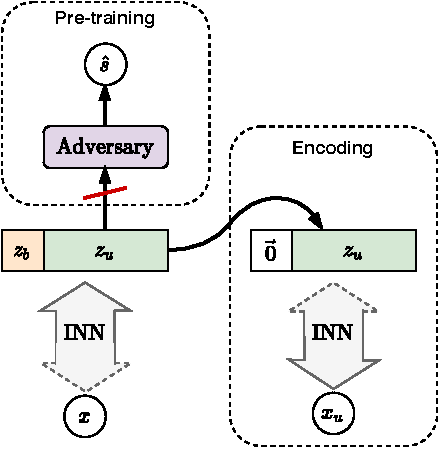
\includegraphics[width=\textwidth]{./Figures/inn_diagram_u.pdf}}%
        \label{fig:inn_diagram}
    }
    \hfill
    \subfloat[cVAE model.]{%
        \scalebox{0.4}{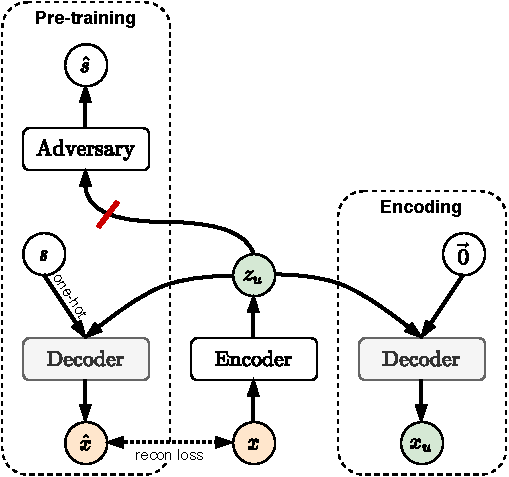
\includegraphics[width=\textwidth]{./Figures/cvae_diagram_u.pdf}}%
        \label{fig:cvae_diagram}
    }
    \hfill
    \caption{
        Training procedure for our models. $x$: input, $s$: sensitive attribute, $z_u$: de-biased representation, $x_u$: de-biased version of the input in the data domain.
        The red bar indicates a gradient reversal layer, and $\stackrel{\rightarrow}{0}$ the null-sampling operation.
    }%
    \label{fig:model-diagrams}
\end{figure*}

\subsection{Problem Statement} % HEADING IS JUST TO HELP ORGANIZE THOUGHTS, WILL BE DELETED LATER
\noindent We assume we are given inputs $\bm{x} \in \mathcal{X}$ and corresponding labels $y \in \mathcal{Y}$.
Furthermore, there is some spurious variable $s \in \mathcal{S}$ associated with each input $\bm{x}$ which we do \emph{not} want to predict. 
Let $X$, $S$ and $Y$ be random variables that take on the values $\bm{x}$, $s$ and $y$, respectively.
The fact that both $y$ and $s$ are predictive of $\bm{x}$ implies that $\mathcal{I}(X;Y), \mathcal{I}(X;S) > 0$, where $\mathcal{I}(\cdot ;\cdot)$ is the mutual information.
Note, however, that the conditional entropy is non-zero: $H(S|X) \neq 0$, i.e., $S$ is not completely determined by $X$.

%The difficulty emerges in the construction of the fully-supervised training dataset in which correspondence between $S$ and $Y$ is exaggerated compared to the test set.
The difficulty of this setup emerges in the training set: there is a close correspondence between $S$ and $Y$, such that for a model that sees the data through the lens of the loss function, the two are indistinguishable.
Furthermore, we assume that this is \emph{not} the case in the test set, meaning the model cannot rely on shortcuts provided by $S$ if it is to generalise from the training set.

We call this scenario where we only have access to the labels of a biasedly-sampled subpopulation
an \emph{aggravated fairness problem}.
These are not uncommon in the real-world.
For instance, in long-feedback systems such as mortgage-approval where the demographics of the subpopulation with observed outcomes is \emph{not} representative of the subpopulation on which the model has been deployed. 
In this case, $s$ has the potential to act as a false (or \emph{spurious}) indicator of the class label and
training a model with such a dataset would limit generalisability.
Let $(X^\mathit{tr}, S^\mathit{tr}, Y^\mathit{tr})$ then be the random variables sampled for the training set
and $(X^\mathit{te}, S^\mathit{te}, Y^\mathit{te})$ be the random variables for the test set.
The training and test sets thus induce the following inequality for their mutual information:
$\mathcal{I}(S^\mathit{tr}; Y^\mathit{tr}) \gg \mathcal{I}(S^\mathit{te}; Y^\mathit{te}) \approx 0$.

% \subsection{In an Ideal World} % HEADING IS JUST TO HELP ORGANIZE THOUGHTS, WILL BE DELETED LATER
Our goal is to learn a representation $\bm{z}_u$ that is independent of $s$ and transferable between downstream tasks.
Complementary to $\bm{z}_u$, we refer to some abstract component of the model that absorbs the unwanted information related to $s$ as $\mathcal{B}$, the realisation of which we define with respect to each of the two models to be described.
%To satisfy this objective, we introduce an additional regularisation term
%that can be viewed from an information-theoretic perspective as minimising the mutual information between the random variables:
The requirement for $\bm{z}_u$ can be expressed via mutual information:
\begin{align}
  I(\bm{z}_u;s) \overset{!}{=} 0~.
  \label{eq:migoal}
\end{align}
However, for the representation to be useful, we need to capture as much relevant information in the data as possible.
Thus, the combined objective function:
\begin{align}
  \min_{\theta} \mathbb{E}_{x \sim X}[-\log p_\theta(\bm{x})] + \lambda I(f_\theta(x);s)
  \label{eq:objectivetheory}
\end{align}
where $\theta$ refers to the trainable parameters of our model $f_\theta$ and $p_\theta(\bm{x})$ is the likelihood it assigns to the data.

We optimise this loss in an adversarial fashion by playing a min-max game, in which our encoder acts as the generative component.
The adversary is an auxiliary classifier $g$, which receives $\bm{z}_u$ as input and attempts to predict the spurious variable $s$.
We denote the parameters of the adversary as $\phi$;
for the parameters of the encoder we use $\theta$, as before.
The objective from~\eqref{eq:objectivetheory} is then% realised as
\begin{align}
  \min_{\theta\in\Theta} \max_{\phi\in\Phi} \mathbb{E}_{x \sim X}[\log p_\theta(x) -\lambda\mathcal{L}_c(g_\phi(f_\theta(x))); s)]
  \label{eq:objectivepractical}
\end{align}
where $\mathcal{L}_c$ is the cross-entropy between the predictions for $s$ and the provided labels.
In practice, this adversarial term is realised with a gradient reversal layer (GRL) \citep{ganin2016domain} between $\bm{z}_u$ and $g$ as is common in adversarial approaches~\citep{edwards2016censoring}.
% to fair representation learning

\subsection{The Disentanglement Dilemma} % HEADING IS JUST TO HELP ORGANIZE THOUGHTS, WILL BE DELETED LATER
The objective in~\eqref{eq:objectivepractical} balances the two desiderata: predicting $y$ and being invariant to $s$.
However, in the training set $(X^\mathit{tr}, S^\mathit{tr}, Y^\mathit{tr})$,
$y$ and $s$ are so strongly correlated that removing information about $s$ inevitably removes information about $y$.
This strong correlation makes existing methods fail under this setting.
% However, this objective is complicated by the desideratum that $\bm{z}_u$ remain predictive of $y$,
% which precludes us from directly training on the target-labelled dataset $(X^\mathit{tr}, S^\mathit{tr}, Y^\mathit{tr})$,
%where $y$ and $s$ are so strongly correlated that removing information about $s$ inevitably removes information about $y$.
%We therefore need
In order to even define the right learning goal,
we require another source of information that allows us to disentangle $s$ and $y$.
For this, we assume the existence of another set of samples that follow a similar distribution to the test set,
but whilst the sensitive attribute is available, the class labels are not.
In reality, this is not an unreasonable assumption,
as, while properly annotated data is scarce, unlabelled data can be obtained in abundance (with demographic information from census data, electoral rolls, etc.).
Previous work has also considered treated ``unlabelled data'' as still having $s$ labels~\citep{wick2019unlocking}.
We are restricted only in the sense that the spurious correlations we want to sever are indicated in the features.
We call this the \emph{representative set}, consisting of $X^\mathit{rep}$ and $S^\mathit{rep}$.
It fulfils $\mathcal{I}(S^\mathit{rep}; Y^\mathit{rep}) \approx 0$
(or rather, it would, if the class labels $Y^\mathit{rep}$ were available).
%{\color{red} justify the existence of such a dataset}

We now summarise the training procedure; an outline for the invertible network model (cFlow) can be seen in Fig.~\ref{fig:inn_diagram}.
First, the encoder network $f$ is trained on ($X^\mathit{rep}, S^\mathit{rep}$), during the first phase.
The trained network is then used to encode the training set,
taking in $\bm{x}$ and producing the representation, $\bm{z}_u$, decorrelated from the spurious variable.
The encoded dataset can then be used to train any off-the-shelf classifier safely, with information about the spurious variable having been absorbed by some auxiliary component $\mathcal{B}$.
In the case of the conditional VAE (cVAE) model,
$\mathcal{B}$ takes the form of the decoder subnetwork, which reconstructs the data conditional on a one-hot encoding of $s$,
while for the invertible network $\mathcal{B}$ is realised as a partition of the feature map $\bm{z}$
(such that $\bm{z} = [\bm{z}_u, \bm{z}_b]$), given the bijective constraint.
Thus, the classifier cannot take the shortcut of learning $s$ and instead must learn how to predict $y$ directly.
Obtaining the $s$-invariant representations, $\bm{x}_u$, in the data domain
is simply a matter of replacing the $\mathcal{B}$ component of the decoder's input for the cVAE,
and $\bm{z}_b$ for cFlow, with a zero vector of equivalent size.
We refer to this procedure used to generate $\bm{x}_u$ as \emph{null-sampling} (here, with respect to $\bm{z}_b)$.

% This That said, we do wish to draw a distinction between null-sampling and the annihilation operation featured in .
Null-sampling resembles the \emph{annihilation} operation described in \citet{xiao2017dna}, however we note that the two serve very different roles.  Whereas the annihilation operation serves as a regulariser to prevent trivial solutions (similar to \cite{jaiswal2018unsupervised}), null-sampling is used to generate the invariant representations post-training.

\subsection{Conditional Decoding}%
\label{conddec}
\noindent We first describe a VAE-based model similar to that proposed in~\citet{madras2018learning}, before highlighting some of its shortcomings that motivate the choice of an invertible representation learner.

The model takes the form of a class conditional $\beta$-VAE \citep{higgins2017beta}, in which the decoder is conditioned on the spurious attribute.
We use $\theta_{enc}, \theta_{dec} \in \theta$ to denote the parameters of the encoder and decoder sub-networks, respectively.
Concretely, the encoder component performs the mapping $x \rightarrow{\bm{z}_u}$, while $\mathcal{B}$ is instantiated as the decoder,
$\mathcal{B} \coloneqq p_{\theta_{dec}}(x|z_u, s)$, which takes in a concatenation of the learned non-spurious latent vector $\bm{z}_u$ and a one-hot encoding of the spurious label $s$ to produce a reconstruction of the input $\hat{x}$.
Conditioning on a one-hot encoding of $s$, rather than a single value, as done in \citet{madras2018learning} is the key to visualising invariant representations in the data domain.
If $\mathcal{I}(z_u; s)$ is properly minimised, the decoder can only derive its information about $s$ from the label, thereby freeing up $\bm{z}_u$ from encoding the unwanted information while still allowing for reconstruction of the input.
Thus, by feeding a zero-vector to the decoder we achieve $\hat{x} \perp s$.
The full learning objective for the cVAE is given as
\begin{align}
\begin{split}
    \mathcal{L}_{\mathrm{cVAE}} =& \mathbb{E}_{q_{\theta_{enc}}(z_u, b|x)}[\log p_{\theta_{dec}}(x|z, b) - \log p_{\theta_{dec}}(s|z_u)] \\ 
    &- \beta D_{KL}(q_{\theta_{enc}}(z_u |x) \| p(z_u))
\end{split}
\end{align}
where $\beta$ is a hyperparameter that determines the trade-off between reconstruction accuracy and independence constraints,
and $p(\bm{z}_u)$ is the prior imposed on the variational posterior.
For all our experiments, $p(\bm{z}_u)$ is realised as an Isotropic Gaussian.
Fig.~\ref{fig:cvae_diagram} summarises the procedure as a diagram.

While we show this setup can indeed work for simple problems, as~\citet{madras2018learning} before us have, we show that it lacks scalability due to disagreement between the components of the loss.
Since information about $s$ is only available to the decoder as a binary encoding,
if the relationship between $s$ and $x$ is highly non-linear and cannot be summarised by a simple on/off mechanism, as is the case if $s$ is an attribute such as gender,
off-loading information to the decoder by conditioning is no longer possible. As a result, $\bm{z}_u$ is forced to carry information about $s$ in order to minimise the reconstruction error. 

The obvious solution to this is to allow the encoder to store information about $s$ in a partition of the latent space as in  \citet{creager2019flexibly}.  However, we question whether an autoencoder is the best choice for this setup, with the view that an invertible model is the better tool for the task. Using an invertible model has several guarantees, namely complete information-preservation and freedom from a reconstruction loss, the importance of which we elaborate on below.

\subsection{Conditional Flow}\label{cflow}
\paragraph{Invertible Neural Networks.}
Invertible neural networks are a class of neural network architecture characterised by a bijective mapping between their inputs and output \citep{Dinh2014}. The transformations are designed such that their inverses and Jacobians are efficiently computable.
These flow-based models permit \emph{exact} likelihood estimation \citep{normflows2015} through the warping of a base density with a series of invertible transformations and computing the resulting, highly multi-modal, but still normalised, density, using the change of variable theorem:
% Flow-GAN \cite{grover2018flowgan} combines the \emph{exact} log-likelihood estimation of the invertible network with the adversarial training of a GAN.
\begin{align}
\begin{split}
  \log p(x) &= \log p(z) + 
   \sum \log \left| \det\left( \frac{\diff h_i}{ h_{i-1}}\right) \right|, %\\
  \quad p(z) = \mathcal{N}(z; 0, \mathbb{I})
  \label{eq:changeofvariables}
\end{split}
\end{align}
where $h_i$ refers to the outputs of the layers of the network and $p(z)$ is the base density, specifically an Isotropic Gaussian in our case.
Training of the invertible neural network is then reduced to maximising $\log p(x)$ over the training set,
i.e.\ maximising the probability the network assigns to samples in the training set.

% The requirement of analytic invertibility and Jacobians demands the use of a specialised subset of neural network layers, but the repertoire of practical invertible transformations has grown steadily over recent years, of which describe only the few we draw upon.

% \paragraph{Coupling layers}. Dinh et al. \cite{Dinh2014} introduced a simple yet powerful invertible transformation in the form of coupling layers. Ease of invertibility is achieved by updating only half of the input vector with a function that itself is trivially invertible but that is at the same time parameterised by a arbitrarily complex operation not subject to the invertibility constraint (e.g. a multi-layer neural network).
% Concretely, the vector $\bm{u}$ is split into two evenly sized vectors: $\bm{u} = [\bm{u}_1, \bm{u}_2]$.
% The output of the coupling layer is then a concatenation of vectors $\bm{v}_1$ and $\bm{v}_2$,
% where $\bm{v}_1 = s \cdot \bm{u}_1 + t$ and $\bm{v}_2 = \bm{u}_2$, with the affine parameters $s$ and $t$ generated by a non-invertible function of $\bm{u}_2$.

% \paragraph{1x1 Convolutions}. Kingma and Dhariwal \cite{KinDha18} introduced invertible 1x1 convolution as a generalised permutation operation and show that determinant can be computed efficiently using an LU decomposition of the weights.

% \paragraph{Spatial downsampling.} To downsample the spatial dimensions and promote mixing between the variables, \cite{Dinh2014} first mask the input with a checkerboard pattern before reshaping (transforming a $c \times h\times w$ tensor into a $4c \times \frac{1}{2} h\times \frac{1}{2}w$). Each "level" of the network is demarcated by a downsampling operation.

\paragraph{The Benefits of Bijectivity.}
Using an invertible network to generate our encoding, $\bm{z}_u$, carries a number of advantages over other approaches.
Ordinarily, the main benefit of flow-based models is that they permit exact density estimation. 
However, since we are not interested in sampling from the model's distribution, in our case the likelihood term serves as a regulariser, as it does for  \citet{JacSmeOya18}. 
Critically, this forces the mean of each latent dimension to zero enabling null-sampling. 
The invertible property of the network guarantees the preservation of all information relevant to $y$ which is independent of $s$, regardless of how it is allocated in the output space.
Secondly, we conjecture that the encodings are more robust to out-of-distribution data.
Whereas an autoencoder could map a previously seen input and a previously unseen input to the same representation,
an invertible network sidesteps this due to the network's bijective property, ensuring all relevant information is stored somewhere. This opens up the possibility of transfer learning between datasets with a similar manifestation of $s$, as we demonstrate in the Appendix~\ref{sec:transfer-learning}.

Under our framework, the invertible network $f$ maps the inputs $\bm{x}$ to a representation $\bm{z}_u$:
$f(\bm{x}) = \bm{z}$.
We interpret the embedding $\bm{z}$ as being the concatenation of two smaller embeddings: $\bm{z} = [\bm{z}_u, \bm{z}_b]$.
The dimensionality of $\bm{z}_b$, and $\bm{z}_u$, by complement, is a free parameter (see section~\ref{sec:optimisation-details} for tuning strategies).
As $f$ is invertible, $\bm{x}$ can be recovered like so:
\begin{align}
  \bm{x} = f^{-1}([\bm{z}_u, \bm{z}_b])
  \label{eq:zreconstruct}
\end{align}
where $\bm{z}_b$ is required for equality of the output dimension and input dimension to satisfy the bijectivity of the network -- we cannot output $\bm{z}_u$ alone, but have to output $\bm{z}_b$ as well. In order to generate the pre-image of $\bm{z}_u$, we perform null-sampling with respect to $\bm{z}_b$ by zeroing-out the elements of $\bm{z}_b$ (such that $\bm{x}_{u} = f^{-1}([\bm{z}_{u}, \stackrel{\rightarrow}{0}])$), i.e. setting them to the mean of the prior density, $\mathcal{N}(z;0, I)$.

How can we be sure that $\bm{z}_u$ contains enough information about $y$?
The importance of the invertible architecture bears out from this consideration. %, as the bijectivity of the network guarantees preservation of all information about the input. %
% The existence of the inverse, $f^{-1}$,  p $x$ from $z$ because $f^{-1}$ exists and can do just that.
As long as $\bm{z}_b$ does not contain the information about $y$, $\bm{z}_u$ necessarily must.
We can raise or lower the information capacity of $\bm{z}_b$ by adjusting its size;
this should be set to the smallest size sufficient to capture all information about $s$, so as not to sacrifice class-relevant information.
Section~\ref{sec:additional-results} explores the effects of the size further.

% Eq~\eqref{eq:zreconstruct} defines how to obtain $\bm{x}$.
% In order to generate the pre-image of $\bm{z}_u$, we perform null-sampling with respect to $\bm{z}_b$ by zeroing-out its elements -- i.e. setting them to the mean of the prior density imposed on $\bm{z}$, $\mathcal{N}(z;0, I)$ -- by the operation, $\bm{x}_{u} = f^{-1}([\bm{z}_{u}, \stackrel{\rightarrow}{0}])$.

% \paragraph{Tuning the Partition Sizes.}

% \paragraph{The Pitfalls of Adversarial Training.}

% \paragraph{Preprocessing}.
% Heuristically, we found that preprocessing the data with an autoencoder stabilises and accelerates training of the cFlow model. The autoencoder was pretrained on the pretraining set solely to minimise reconstruction loss and its weights frozen at the time of the INN's training. While this means the INN is not truly lossless with respect to the uncompressed data, its bijectivity is leveraged to ensure semantically-relevant information is not discarded during the pre-training phase, which is still applicable since the autoencoder is not trained jointly with the INN to maximise the adversarial loss. Since the autoencoder is optimised for compression, information about both the spurious and non-spurious attributes is captured impartially in its encoding.

%%%%%%%%% Experiments

\section{Experiments}
\noindent We present experiments to demonstrate that the null-sampled representations are in fact invariant to $s$
while still allowing a classifier to predict $y$ from them.
We run our cVAE and cFlow models on the coloured MNIST (cMNIST) and CelebA dataset,
which we artificially bias, first describing the sampling procedure we follow to do so for non-synthetic datasets.
As baselines we have the model of~\citet{kim2019learning} (Ln2L) and the same CNN used to evaluate the cFlow and cVAE models
but with the unmodified images as input (CNN).
For the cFlow model we adopt a Glow-like architecture~\citep{KinDha18},
while both subnetworks of the cVAE model comprise gated convolutions~\citep{van2016conditional}, where the encoding size is $256$.
For cMNIST, we construct the Ln2L baseline according to its original description, for CelebA,
we treat it as an augmentation of the baseline CNN's objective function.
%More
Detailed information regarding model architectures can be found in sections~\ref{sec:architectures} and~\ref{sec:optimisation-details}.%
\footnote{The code can be found at \url{https://github.com/predictive-analytics-lab/nifr}.}
% \begin{figure*}[!htb]
%   \centering
%   %
%   \subfloat[CelebA]{\scalebox{0.495}{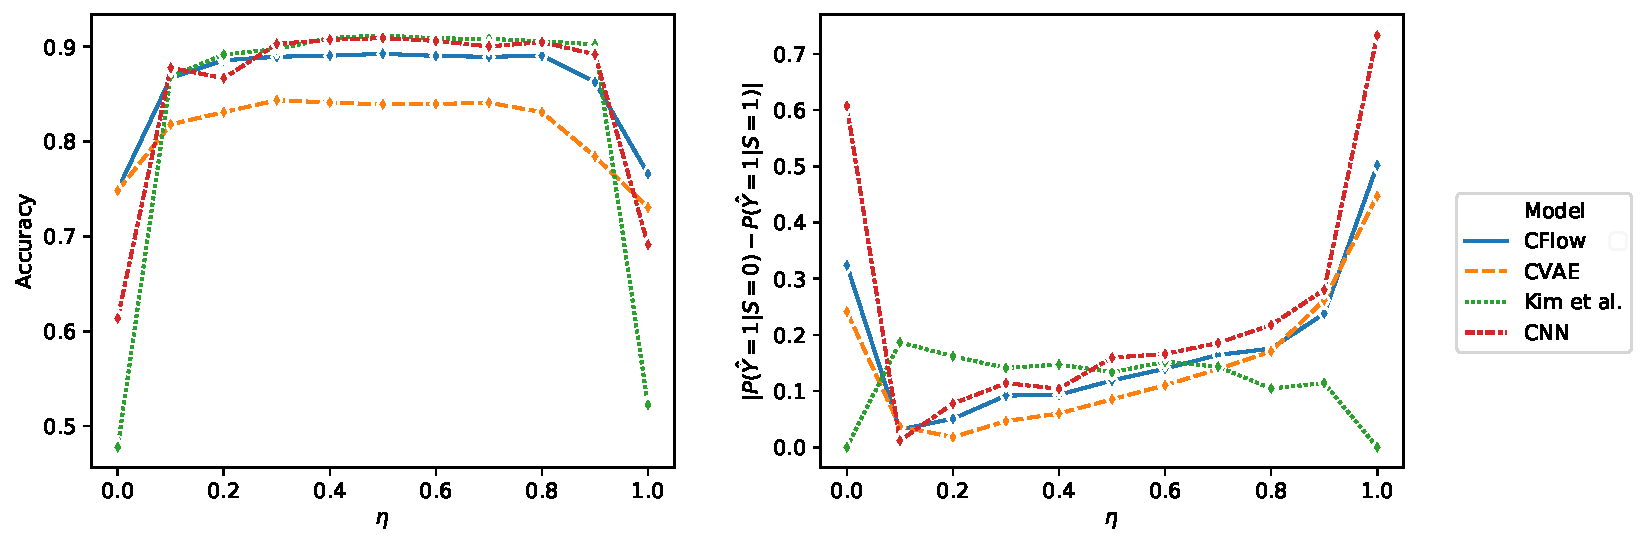
\includegraphics[width=\textwidth]{./results/celeba/celeba_acc_DP.pdf}}
%   \label{fig:celeba_chart}
%   }%
%   %\hfill
%   \subfloat[UCI Adult]{\scalebox{0.495}{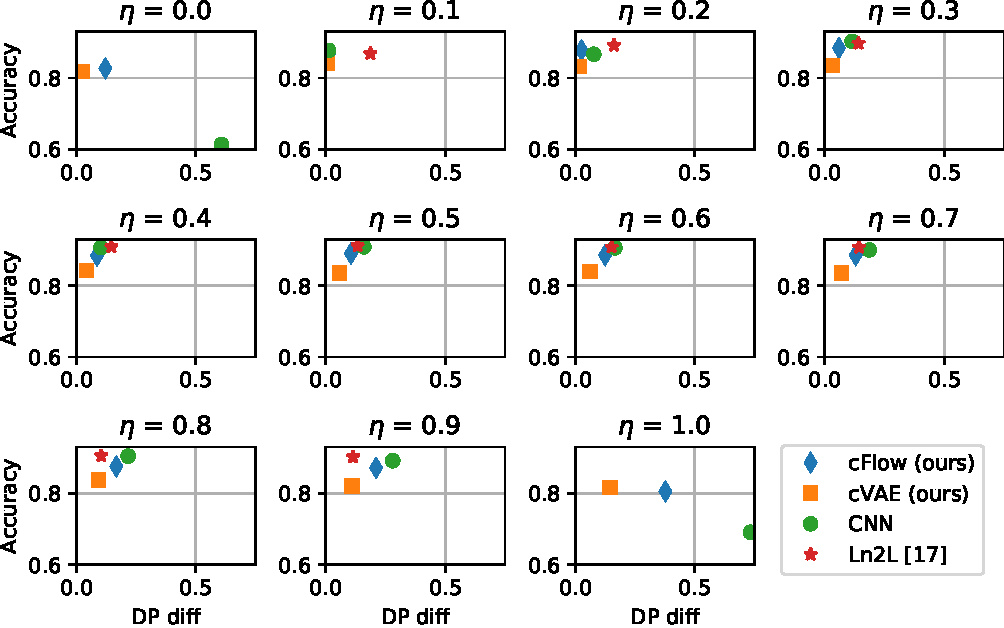
\includegraphics[width=\textwidth]{paper2/Figures/nosinn_celeba_multiplot_all_landscape_Smiling.pdf}}
%   \label{fig:adult_chart}
%   }%
%   \caption{
%     Performance of our approach on the CelebA and UCI Adult datasets.
%     (Left of each) We show the accuracy of a downstream classifier trained on representations learned by our model.
%     (Right of each) We show the Demographic Parity of a model trained on our representations (the lower the better).
%   }\label{fig:chart}
% \end{figure*}
\begin{figure}[tb]
    \centering
    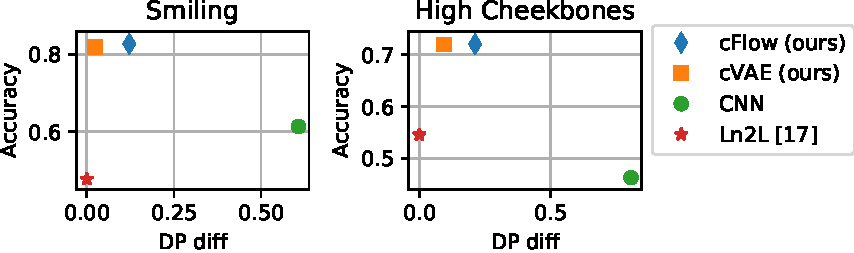
\includegraphics[width=0.7\textwidth]{paper2/Figures/nosinn_celeba.pdf}
    \caption{
        Performance of our model for different targets (mixing factor $\eta=0$).
        Left: \emph{Smiling} as target, right: \emph{high cheekbones}.
        \emph{DP diff} measures fairness with respect to demographic parity.
        A perfectly fair model has a \emph{DP diff} of 0.
    }%
    \label{fig:celeba-targets}
\end{figure}

\begin{figure}[tb]
    \centering
    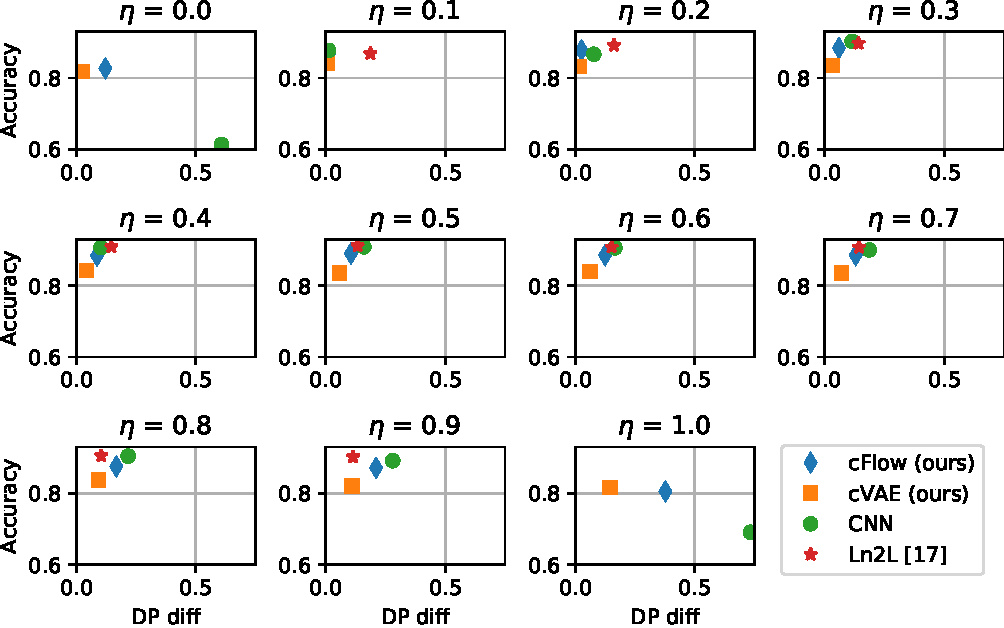
\includegraphics[width=0.85\textwidth]{paper2/Figures/nosinn_celeba_multiplot_all_landscape_Smiling.pdf}
    \caption{
        Performance of our model for the target ``smiling'' for different mixing factors $\eta$.
        \emph{DP diff} measures fairness with respect to demographic parity.
        A perfectly fair model has a \emph{DP diff} of 0, thus the closer to top-left the better it is in terms of we accuracy-fairness trade-off.
        Only values $\eta=0$ and $\eta=1$ correspond to the scenario of a strongly biased training set.
        The results for $0.1\leq \eta\leq 0.9$ are to confirm that our model does not harm performance for non-biased training sets.
    }%
    \label{fig:celeba-multiplot}
\end{figure}

% \begin{figure*}[!htb]
%   \centering
%   \caption{Performance of our methods (cVAE and cFlow) on the tabular UCI Adult Dataset. This is a common benchmark in fair machine learning literature. Each model depicts the result of a ownstream classifier trained on the embeddings produced by one of the models. (Left) Accuracy of a downstream classifier. (Middle) Demographic Parity of a downstream classifier. (Right) Equality of Opportunity of a downstream classifier.}\label{fig:adult_results}
% \end{figure*}
\subsection{Synthesising Dataset Bias}
For our experiments, we require a training set that exhibits a strong spurious correlation, together with a test set that does not.
For cMNIST, this is easily satisfied as we have complete control over the data generation process.
For CelebA and  UCI Adult, on the other hand,
we have to generate the split from the existing data.
To this end, we first set aside a randomly selected portion of the dataset from which to sample the biased dataset
The portion itself is then split further into two parts:
one in which $(s=-1 \land y=-1) \lor (s=+1 \land y=+1)$ holds true for all samples, call this part $\mathcal{D}_{eq}$,
and the other part, call it $\mathcal{D}_{opp}$, which contains the remaining samples.
To investigate the behaviour at different levels of correlation,
we mix these two subsets according to a mixing factor $\eta$.
For $\eta \leq \tfrac{1}{2}$, we combine (all of) $\mathcal{D}_{eq}$
with a fraction of $2\eta$ from $\mathcal{D}_{opp}$.
For $\eta > \tfrac{1}{2}$, we combine (all of) $\mathcal{D}_{opp}$
and a fraction of $2(1 -\eta)$ from $\mathcal{D}_{eq}$.
Thus, for $\eta=0$, the biased dataset is just $\mathcal{D}_{eq}$,
for $\eta=1$ it is just $\mathcal{D}_{opp}$
and for $\eta=\tfrac{1}{2}$ the biased dataset is an ordinary subset of the whole data. The test set is simply the data remaining from the initial split.

\subsection{Evaluation protocol}
We evaluate our results in terms of accuracy and fairness.
A model that perfectly decouples its predictions from $s$ will achieve near-uniform accuracy across all biasing-levels.
For binary $s$/$y$ we quantify the fairness of a classifier's predictions using \emph{demographic parity} (DP): the  absolute difference in the probability  of a positive prediction for each sensitive group.

% We also calculate the absolute difference in Equality of Opportunity \cite{hardt2016equality}, which is the relationship between True Positive Rates of subgroups with the same sensitive attribute.

\begin{figure}[tb]
    \centering
    % 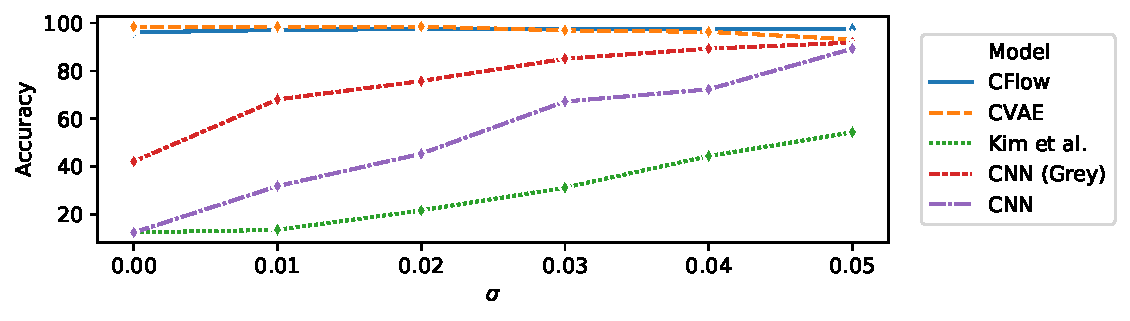
\includegraphics[width=0.9\textwidth]{./results/cmnist/cmnist_results.pdf}
    % 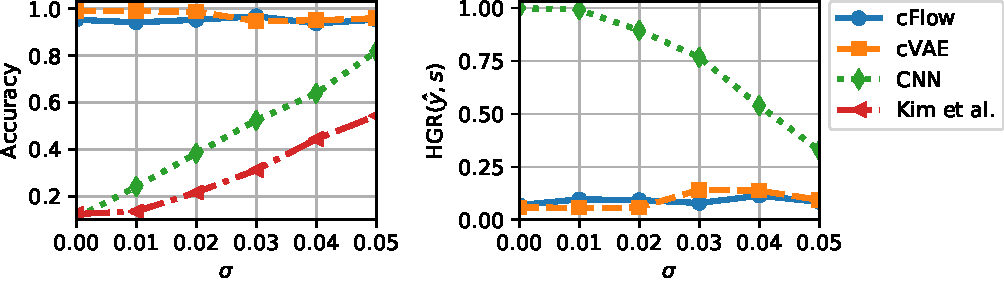
\includegraphics[width=0.9\textwidth]{paper2/Figures/cmnist_new.pdf}
    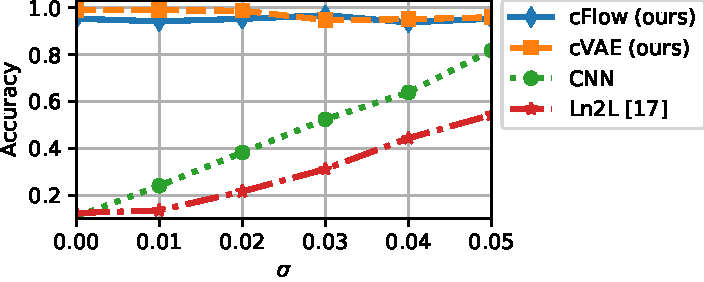
\includegraphics[width=0.7\textwidth]{paper2/Figures/cmnist_new_no_hgr.pdf}
    \caption{
        % Accuracy and correlation (HGR) of predictions $\hat{y}$ and $s$ of our approach in comparison with other baseline models on the cMNIST dataset, for different standard deviations ($\sigma$) for the colour sampling.
        Accuracy of our approach in comparison with other baseline models on the cMNIST dataset, for different standard deviations ($\sigma$) for the colour sampling.
    }%
    \label{fig:cmnist_chart}
\end{figure}
\subsection{Experimental results}
% \noindent Our model can be applied to tabular data and image data alike.
% Due to space constraints, the experiments with the tabular dataset \emph{UCI Adult} are situated in the Appendix.
%To illustrate the effectiveness and generality of our framework, we apply our models to a tabular dataset, in the UCI Adult dataset,
We report the results from two image datasets.
cMNIST, a synthetic dataset, is a good starting point for evaluating our model due to the direct control we have over the biasing.
CelebA, on the other hand, is a more practical and challenging example.
% To illustrate the generality of our approach,
We also test our method on a tabular dataset, the Adult dataset.
%For full details regarding the architectures of our models and their optimisation, see the Appendix.

\paragraph{cMNIST.}
The coloured MNIST (cMNIST) dataset is a variant of the MNIST dataset in which the digits are coloured.
In the training set, the colours have a one-to-one correspondence with the digit class.
In the test set (and the representative set), colours are assigned randomly.
The colours are drawn from Gaussians with 10 different means.
We follow the colourisation procedure outlined by~\citet{kim2019learning}, with the mean colour values selected so as to be maximally dispersed.
The full list of such values can be found in section~\ref{sec:color-details}.
We produce multiple variants of the cMNIST dataset corresponding to different standard deviations $\sigma$ for the colour sampling:
$\sigma \in \{0.00, 0.01, ..., 0.05 \}$.
% The images are symmetrically zero-padded to a size of $32 \times 32$ to allow for an additional downsampling stage in the cFlow model.
% No additional data augmentation is used.
% 24,000 of the 36,000 training samples were set aside for representative, the remaining 10,000 for training the downstream classifier.
% We continue to use 10,000 samples usually reserved for testing on vanilla MNIST for that same purpose.

For this specific dataset, we can establish an additional baseline by simply grey-scaling the dataset
% Since the data-generation process is known, we can establish a baseline an additional by following the simple heuristic of grey-scaling the dataset
which only leaves the luminosity as spurious information.
%The grey-scaling operation does not completely eliminate the bias in the dataset, it only mitigates it by reducing the number of unique values for $s$ it is still exhibited residually in the luminosity of the digits.
We also evaluate the model, with all the associated hyperparameters, from~\citet{kim2019learning}.
The only difference between the setups is the dataset creation, including the range of $\sigma$ values we consider.
Our versions of the dataset, on the whole, exhibit much stronger colour bias, to the point of the mapping the digit's colour and class being bijective.
Fig.~\ref{fig:cmnist_chart} shows that the model significantly underperforms even the na\"ive baseline, aside from at $\sigma = 0$, where they are on par.

Inspection of the null-samples shows that both the cVAE and cFlow model succeed in removing almost all colour information, which is supported quantitatively by fig.~\ref{fig:cmnist_chart}.
While the cVAE outperforms cFlow marginally at low $\sigma$ values, performance degrades
%rapidly
as this increases.
This highlights the problems with the conditional decoder we anticipated in section~\ref{conddec}.
The lower $\sigma$, and therefore the variation in sampled colour, is, the more reliably the $s$ label, corresponding to the mean of RGB distribution, encodes information about the colour.
For higher $\sigma$ values, the sampled colours can deviate far from the mean and so the encoder must incorporate information about $s$ into its representation if it is to minimise the reconstruction loss.
cFlow, on the other hand, is consistent across $\sigma$ values.

\paragraph{CelebA.}
To evaluate the effectiveness of our framework on real-world image data we use the CelebA dataset~\citep{liu2015faceattributes}, consisting of 202,599 celebrity images.
These images are annotated with various binary physical  attributes, including ``gender'', ``hair colour'', ``young'', etc, from which we  select our sensitive and target attributes.
The images are centre cropped and resized to $64\times64$, as is standard practice.
For our experiments, we designate ``gender'' as the sensitive attribute,
and ``smiling'' and ``high cheekbones'' as target attributes.
We chose gender as the sensitive attribute as it a common sensitive attribute in the fairness literature.
For the target attributes, we chose attributes that are harder to learn than gender and which do not correlate too strongly with gender in the dataset
(``wearing lipstick'' for example being an attribute too closely correlated with gender).
% The sampling and evaluation procedure is identical to that conducted for the UCI Adult dataset.
% We evaluate the performance of all models for mixing factors ($\eta$) of value $\{0, 0.1, ..., 1\}$. 
The model is trained on the representative set (normal subset of CelebA)
and is then used to encode the artificially biased training set and the test set.
The results for the most strongly biased training set ($\eta=0$) can be found in fig.~\ref{fig:celeba-targets}.
Our method outperforms the baselines in accuracy and fairness.

We also assess performance for different mixing factors ($\eta$) which correspond to varying degrees of bias in the training set
(see fig.~\ref{fig:celeba-multiplot}).
This is to verify that the model does not \emph{harm} performance when there is not much bias in the training set.
For these experiments, the model is trained once on the representative set and is then used to encode different training sets.
The results show that for the intermediate values of $\eta$, our model incurs a small penalty in terms of accuracy,
but at the same time makes the results \emph{fairer} (corresponding to an accuracy-fairness trade-off). Qualitative results can be found in fig.~\ref{fig:celeba_cflow} (images from cVAE can be found in section~\ref{sec:qual-results-celeba}).

To show that our method can handle multinomial, as well as binary, sensitive attributes, we also conduct experiments with $s=\textrm{hair colour}$ as a ternary attribute (``Blonde'', ``Black'', ``Brown''), excluding ``Red'' because of the paucity of samples and the noisiness of their labels. The results for these experiments can be found in section~\ref{sec:additional-results}.
% Looking at the produced invariant representations,
% The failure of the cVAE to model complex interactions between $x_u$ and $s$ is brought to bear here.
% Due to the balancing between the adversarial and reconstruction losses,
% information relevant to the downstream task of predicting ``smiling'' is lost during the pre-training phase,
% leading to poor performance at all values of $\eta$ except the most extreme ones,
% for which it does reasonably well at mitigating the sampling bias (Fig.~\ref{fig:celeba_chart}).
% Meanwhile, cFlow does not suffer this drawback -- the images remain sharp
% (see Fig.~\ref{fig:cflow_celeba_recon_y} in comparison to Fig. \ref{fig:cvae_celeba_recon_y})
% and the accuracy obtained by training on them is comparable to the baseline at intermediary values -- and at the same time matches and outperforms the cVAE at $\eta = 0$ and $\eta = 1$, respectively.
% For these same values,
% incorporating the mutual information loss proposed by~\cite{kim2019learning} into the classifier's loss function greatly harmed performance measured by accuracy;
% the DP is zero due to all predictions being negative.

% \begin{wrapfigure}{l}{0.6\linewidth}
\begin{figure}[tb]
  \centering
  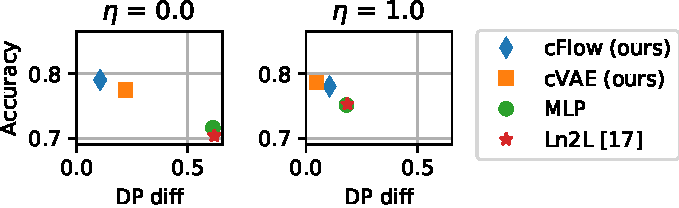
\includegraphics[width=0.6\textwidth]{paper2/Figures/nosinn_adult_multiplot_mini_diff.pdf}
  \caption{
      Results for the \textsc{Adult} dataset.
      The $x$-axis corresponds to the difference in positive rates.
      An ideal result would occupy the \textsc{top-left}.
  }%
  \label{fig:adult-chart}
\end{figure}
% \end{wrapfigure}

\paragraph{Results for the UCI Adult dataset.}
The UCI Adult dataset consists of census data and is commonly used to evaluate models focused on algorithmic fairness.
Following convention, we designate ``gender'' as the sensitive attribute $s$ and whether an individual's salary is \$50,000 or greater as $y$.
We show the performance of our approach in comparison to baseline approaches in fig. \ref{fig:adult-chart}.
We evaluate the performance of all models for mixing factors ($\eta$) $0$ and $1$. 
Results shown in fig. \ref{fig:adult-chart} show that
%while our model fails to surpass the baseline models in terms of accuracy for the balanced case (and those close to it),
we match or exceed the baseline.
%as $\eta$ moves the dataset towards a more imbalanced setting.
In terms of fairness metrics, our approach generally outperforms the baseline models for both of $\eta$.
Detailed results can be found in section~\ref{sec:additional-results}.

We also did experiments to show that the encoder transfers to other tasks. These transfer-learning experiments can be found in section~\ref{sec:transfer-learning}.


% \begin{figure}
%   \centering
%   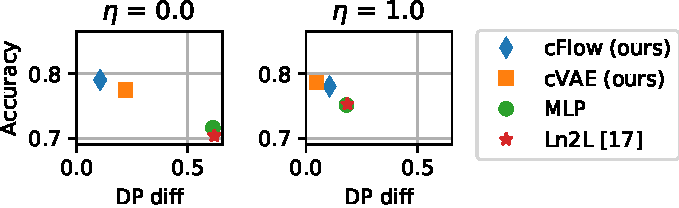
\includegraphics[width=0.7\textwidth]{paper2/Figures/nosinn_adult_multiplot_mini_diff.pdf}
%   \caption{
    %   Results for the \textsc{Adult} dataset.
    %   The $x$-axis corresponds to the difference in positive rates.
    %   An ideal result would occupy the \textsc{top-left}.
%   }%
%   \label{fig:adult-chart}
% \end{figure}

\section{Conclusion}\label{sec:conclusion}
%%%%%%%%%%%%% DISCUSSION %%%%%%%%%%%%%%%
% Controlling the correlations a computer vision and machine learning system discovers is known to be a difficult problem.
% Recent work~\cite{JoBen17,GatEckBet17,JacBehZemBet19} has shown that state-of-the-art deep convolutional neural network (CNN) systems strongly rely on \emph{shortcuts}. 
% Examples of these shortcuts include spectral statistical regularities and stationary statistics such as colours and textures. 
% Indeed, it has been shown that standard ImageNet-trained classifiers place much more weight on object textures compared to object shapes \cite{Geir18}.  As discussed in \cite{zhang2018examining} the representation flaws that result from these shortcuts can be difficult to pick up on because the test images may exhibit a similar bias.
% Those systems rely less on higher-level abstract concepts such as shape and appearance than on such details highly-correlated with, but unconnected to the classification.
% While this may be acceptable, and even desirable in certain cases (e.g. when combining image content and style from two separate images \cite{gatys2016image}), to achieve robustness, machine learning models have to look beyond \emph{spurious} correlations to those that hold true regardless of context.
% By doing so, the system can learn to produce accurate and reliable predictions, even when deployed in settings radically different from the one in which it was trained.
% However, if the training set contains spurious correlations, then a computer vision and machine learning system cannot learn the true relations just from that dataset.
% We either need to supply an inductive bias \cite{locatello2019challenging} or additional information which we can incorporate into learning.

% As a step towards solving these problems,
We have proposed a general and straightforward framework for producing invariant representations, under the assumption that a representative but partially-labelled \emph{representative} set is available.
Training consists of two stages:
an encoder is first trained on the representative set to produce a representation that is invariant to a designated spurious feature. 
This is then used as input for a downstream task-classifier, the training data for which might exhibit extreme bias with respect to that feature.
We train both a VAE- and INN-based model according to this procedure, and show that the latter is particularly well-suited to this setting due to its losslessness. 
The design of the models allows for representations that are in the data domain and therefore exhibit meaningful invariances. 
We characterise this for synthetic as well as real-world datasets for which we develop a method for simulating sampling bias.

\section*{Acknowledgements}
This work was in part funded by the European Research Council 
under the ERC grant agreement no. 851538.
We are grateful to NVIDIA for donating GPUs.

% updated April 2002 by Antje Endemann
% Based on CVPR 07 and LNCS, with modifications by DAF, AZ and elle, 2008 and AA, 2010, and CC, 2011; TT, 2014; AAS, 2016; AAS, 2020

% \documentclass[runningheads]{llncs}
% \usepackage{graphicx}
% \usepackage{comment}
% \usepackage{amsmath,amssymb,amsfonts,bm} % define this before the line numbering.
% \usepackage{color}
% \usepackage{tabularx}
% \usepackage{appendix}

% % our packages
% \usepackage{import}
% % \usepackage{subcaption}
% \usepackage[caption=false]{subfig}
% \usepackage{mathtools}
% \usepackage{booktabs}

% INITIAL SUBMISSION - The following two lines are NOT commented
% CAMERA READY - Comment OUT the following two lines
% \usepackage{ruler}
% \usepackage[width=122mm,left=12mm,paperwidth=146mm,height=193mm,top=12mm,paperheight=217mm]{geometry}

% Macros
% \def\ci{\perp\!\!\!\perp}
% \newcommand*\diff{\mathop{}\!\mathrm{d}}
% \def\httilde{\mbox{\tt\raisebox{-.5ex}{\symbol{126}}}}


% \begin{document}
% \renewcommand\thelinenumber{\color[rgb]{0.2,0.5,0.8}\normalfont\sffamily\scriptsize\arabic{linenumber}\color[rgb]{0,0,0}}
% \renewcommand\makeLineNumber {\hss\thelinenumber\ \hspace{6mm} \rlap{\hskip\textwidth\ \hspace{6.5mm}\thelinenumber}}
% \linenumbers
% \pagestyle{headings}
% \mainmatter
% \def\ECCVSubNumber{5488}  % Insert your submission number here

% \title{Null-sampling for Interpretable and \\Fair Representations -- Appendix} % Replace with your title

% % INITIAL SUBMISSION 
% \begin{comment}
% \titlerunning{ECCV-20 submission ID \ECCVSubNumber} 
% \authorrunning{ECCV-20 submission ID \ECCVSubNumber} 
% \author{Anonymous ECCV submission}
% \institute{Paper ID \ECCVSubNumber}
% \end{comment}
% %******************

% % CAMERA READY SUBMISSION
% %\begin{comment}
% \titlerunning{Appendix}
% % If the paper title is too long for the running head, you can set
% % an abbreviated paper title here
% %
% \author{Thomas Kehrenberg \and
% Myles Bartlett \and
% Oliver Thomas \and \\
% Novi Quadrianto}
% %
% \authorrunning{T. Kehrenberg et al.}
% % First names are abbreviated in the running head.
% % If there are more than two authors, 'et al.' is used.
% %
% \institute{Predictive Analytics Lab (PAL), University of Sussex, Brighton, UK
% \email{\{t.kehrenberg,m.bartlett,ot44,n.quadrianto\}@sussex.ac.uk}}
% %\end{comment}
% %******************

% \title{Appendix}
% \author{}
% \institute{}
% \maketitle
% \thispagestyle{headings}

\section{Appendix}\label{sec:nifr-appendix}

% \begin{appendix}

\subsection{Model Architectures}%
\label{sec:architectures}
\noindent For both cMNIST and CelebA we parameterise the coupling layers with the same convolutional architecture as in \citet{KinDha18}, consisting of $3$ convolutional layers each with $512$ filters of, in order, sizes $3\times3$, $1\times1$, and $3\times3$.
Following \citet{ardizzone2019guided}, we Xavier initialise all but the last convolutional layer of the $s$ and $t$ sub-networks which itself is zero-initialised so that the coupling layers begin by performing an identity transform. We used a Glow-like architecture \citep{KinDha18} (affine coupling layers together with checkerboard reshaping and invertible $1\times1$ convolutions) for the convolutional INNs. Table \ref{tab:inn_architectures} summarises the INN architectures used for each dataset.

For the image datasets each level of the cVAE encoder consists of two gated convolutional layers \citep{van2016conditional} with ReLU activation. 
At each subsequent level, the number of filters is doubled, starting with an initial value 32 and 64 in the case of CelebA and cMNIST respectively. 
In the case of the Adult dataset, we use an encoder with one fully-connected hidden layer of width $35$, followed by SeLU activation \citep{klambauer2017self}. 
For both cMNIST and CelebA, we downsample to a feature map with spatial dimensions $8\times8$, but with $3$ and $16$ channels respectively. 
For the Adult dataset, the encoding is a vector of size $35$. 
The output layer specifies both the parameters (mean and variance) of the representation's distribution. 
In all cases the KL-divergence is computed with respect to a standard isotropic Gaussian prior. 
Details of the encoder architectures can be found in table \ref{tab:vae_architectures}. The loss pre-factors were sampled from a logarithmic scale; without proper balancing the networks can exhibit instability, especially during the early stages of training.

\begin{table}[tp]
\caption{INN architecture used for each dataset.}
\label{tab:inn_architectures}
\centering
\begin{tabular}{lllll}
\toprule
Dataset & Levels & Level depth & Coupl. chan. & Input to discr. \\ \midrule
UCI Adult                   & 1      & 1     & 35       & Null-samples       \\
cMNIST                      & 3      & 16     & 512      & Encodings               \\
CelebA                      & 3      & 32     & 512      & Encodings        \\ \bottomrule
\end{tabular}
\end{table}

\begin{table}[tp]
\caption{cVAE encoder architecture used for each dataset. The decoder architecture in each case mirrors that of its encoder counterpart through use of transposed convolutions. For the adult dataset we apply $\ell_2$ and cross-entropy losses to the reconstructions of the continuous features and discrete features, respectively.}
\label{tab:vae_architectures}
\centering
\begin{tabular}{lllll}
\toprule
Dataset   & Initial channels & Levels & $\beta$ & Recon. loss \\
\midrule
UCI Adult & 35               & --     & 0       & $\ell_2$ + CE\\
cMNIST    & 32               & 4      & 0.01    & $\ell_2$ \\
CelebA    & 32               & 5      & 1       & $\ell_1$ \\ 
\bottomrule
\end{tabular}
\end{table}

\subsection{Instructions for potential users}
The first question a potential user has to ask themselves is
whether the method is a good fit:
is the problem that the user faces one of strong spurious correlation
and is there non-spurious data available that has labels for the spurious variable?
To investigate the first part of the question,
the user should first try to train a standard neural network classifier
and observe the test-set performance.
Furthermore, one should check
whether the spurious variable can be removed with data augmentations alone.

to use the cFlow or cVAE variant of the method.
For initial experiments, we would recommend the cVAE model as it is quicker to train,
and will lead to shorter feedback cycles when validating the code.
If the computational budget allows it,
we would recommend switching to the cFlow model once cVAE is working
as it provides better guarantees regarding the retention of information from the input data.

\subsection{Additional results}\label{sec:additional-results}
\paragraph{Detailed results for UCI Adult dataset.}
This census data is commonly used to evaluate models focused on algorithmic fairness.
Following convention, we designate ``gender'' as the $s$ and whether an individual's salary is \$50,000 or greater as $y$.
We show the performance of our approach in comparison to baseline approaches in fig.~\ref{fig:big-adult-chart}.
We evaluate the performance of all models for mixing factors ($\eta$) of value $\{0, 0.1, ..., 1\}$. 
Results shown in fig.~\ref{fig:big-adult-chart} show that whilst our model fails to surpass the baseline models in terms of accuracy for the balanced case (and those close to it), we match or exceed the baseline as $\eta $ moves the dataset to a more imbalanced setting. In terms of fairness metrics,  our approach generally outperforms the baseline models regardless of $\eta$.

\begin{figure}[htb]
  \centering
  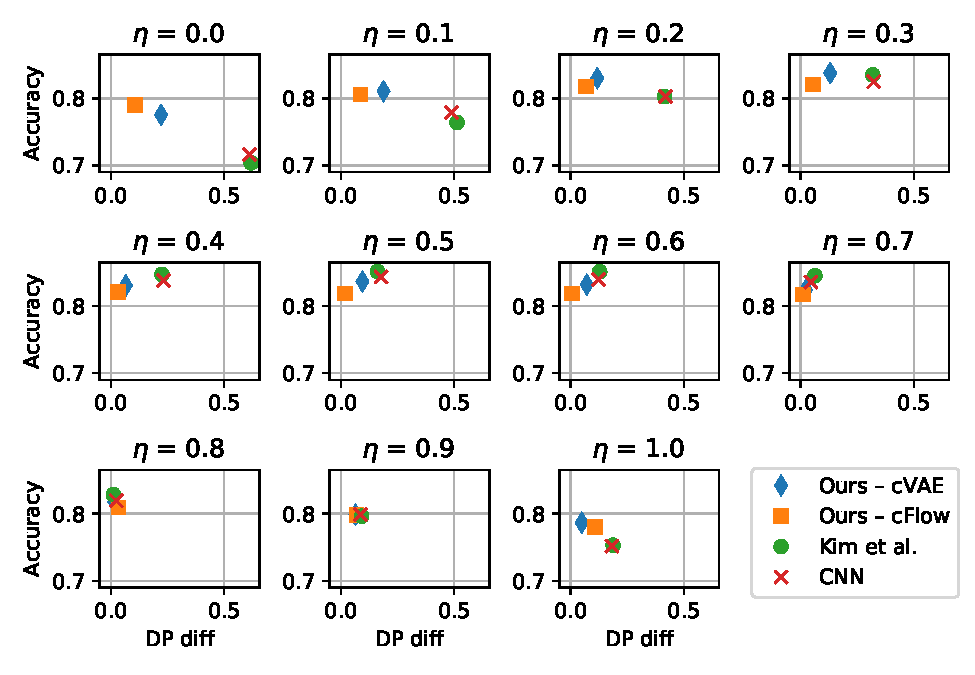
\includegraphics[width=0.85\textwidth]{paper2/Figures/nosinn_adult_multiplot_all_landscape_diff.pdf}
  \caption{
      Results for the \textsc{Adult} dataset.
      The $x$-axis corresponds to the difference in positive rates.
      An ideal result would occupy the \textsc{top-left}.
  }%
  \label{fig:big-adult-chart}
\end{figure}
\begin{figure}[htb]
    \centering
    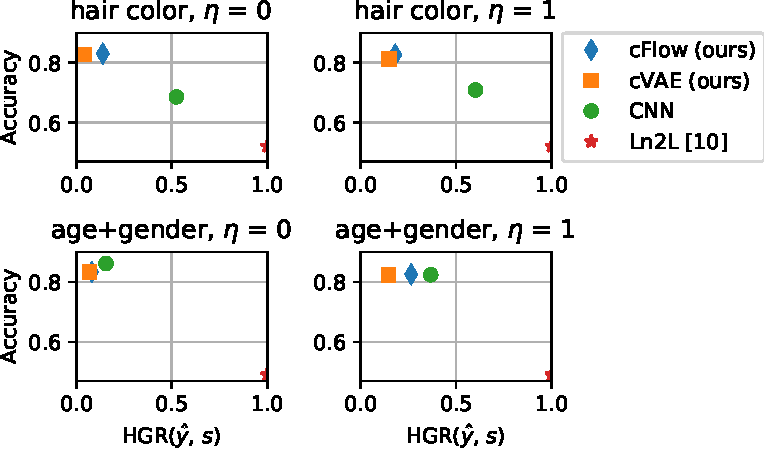
\includegraphics[width=0.7\textwidth]{paper2/Figures/celeba_multi_s.pdf}
    \caption{
        For \emph{hair colour}, $s$ takes on the values Blond, Brown and Black.
        For \emph{age+gender}, $s$ takes on the values Young/Female, Young/Male, Old/Female and Old/Male.
    }%
    \label{fig:multi-s}
\end{figure}

\paragraph{Multinomial sensitive attributes.}
In addition to binary sensitive attribute $s$,
we also investigate multinomial $s$ in the CelebA dataset.
First, we do experiments with hair colour, where $s$ has three possible values:
blond hair, brown hair and black hair.
The other experiment is with a combination of age and gender,
where $s$ has four possible values, each of which is a combination of a gender and an age:
Young/Female, Young/Male, Old/Female and Old/Male.
To evaluate the fairness for multinomial $s$, we use the Hirschfeld-Gebelein-R\'enyi Maximum Correlation Coefficient (HGR) \citep{mary2019fairness} that is defined on the domain $[0, 1]$ and gives $\text{HGR}(Y,S)=0$ iff $Y \perp S$
and 1 if there is a deterministic function to map between them.
Results can be found in figure~\ref{fig:multi-s}.\\

\begin{table}[tp]
\caption{Results on the CelebA dataset with different sizes of $z_b$.}
    \label{tab:zs-ablation}
    \centering
\begin{tabular}{l@{\extracolsep{1cm}}lrr}
\toprule
 $|z_b|$ & $|z_b|/|z|$ &  Accuracy &   DP diff \\
\midrule
          1 &             0.0082\% &  0.60 &  0.63 \\
          3 &             0.0245\% &  0.60 &  0.63 \\
          5 &             0.0410\% &  0.84 &  0.12 \\
         10 &             0.0820\% &  0.84 &  0.12 \\
         30 &             0.2442\% &  0.74 &  0.23 \\
         50 &             0.4070\% &  0.68 &  0.27 \\
\bottomrule
\end{tabular}
\end{table}
\noindent\textsc{Investigation into the size of $z_b$.}
\;\; In the cFlow model, the size of $z_b$ is an important hyperparameter which can affect the result significantly.
Here we investigate the sensitivity of the model to the choice of $z_b$ size.
Table~\ref{tab:zs-ablation} shows accuracy and fairness (as measured by \emph{DP diff}) for different sizes of $z_b$.
The results show that both too large and too small $z_b$ is detrimental.
However, they also show that the model is not overly sensitive to this parameter:
both sizes 5 and 10 achieve nearly identical results.

\begin{table}[tbp]
    \caption{
        Additional fairness metrics for the experiments on the CelebA dataset (fig.~\ref{fig:celeba-multiplot} from the main text).
        \emph{TPR diff.}\ refers to the difference in true positive rate.
        \emph{TNR diff.}\ refers to the difference in true negative rate.
        \textsc{Left:} $\eta = 0$. \textsc{Right:} $\eta=1$.
    }
    \label{tab:my_label}
    \resizebox{.49\textwidth}{!}{
    \begin{tabular}{lrrrr}
\toprule
     Method &  Accuracy &  DP diff &  TPR diff &  TNR diff \\
\midrule
      cFlow &      0.83 &     0.10 &      0.15 &      0.25 \\
       cVAE &      0.82 &     0.05 &      0.09 &      0.18 \\
        CNN &      0.61 &     0.63 &      0.70 &      0.64 \\
 Ln2L &      0.52 &     0.00 &      0.00 &      0.00 \\
\bottomrule
\end{tabular}}
\hfill
\resizebox{.49\textwidth}{!}{
\begin{tabular}{lrrrr}
\toprule
     Method &  Accuracy &  DP diff &  TPR diff &  TNR diff \\
\midrule
      cFlow &      0.82 &     0.33 &      0.28 &      0.21 \\
       cVAE &      0.81 &     0.16 &      0.10 &      0.05 \\
        CNN &      0.67 &     0.75 &      0.66 &      0.76 \\
Ln2L &      0.51 &     0.08 &      0.06 &      0.09 \\
\bottomrule
\end{tabular}}
\end{table}
\paragraph{Additional fairness metrics.}
In addition to \emph{DP diff}, we report here the result from other fairness measures.
These results are from the same setup as those reported in the main paper.
We report the difference in true positive rates (TPR) between the two groups (male and female), which corresponds to a measure of Equality of Opportunity,
and the difference in true negative rates (TNR) between the two groups.

\subsection{Optimisation Details}\label{sec:optimisation-details}
\noindent All our models were trained using the RAdam optimiser \citep{liu2019variance} with learning rates $3\times10^{-4}$ and $1\times10^{-3}$ for the encoder/discriminator pair and classifier respectively. A batch size of 128 was used for all experiments.

We now detail the optimisation settings, including the choice of adversary, specific to each dataset. Details of the cVAE and cFlow architectures can be found in table \ref{tab:vae_architectures} and table \ref{tab:inn_architectures}, respectively.

\paragraph{UCI Adult.} 
For this dataset our experiment benefited from using null-samples as inputs to the adversary of the cFlow model. Unlike for the image datasets, we found a single adversary to be sufficient. This was realised as a multi-layer perceptron (MLP) with one hidden layer, 256 units wide. The INN performs a bijection of the form $f: \mathbb{R}^n \rightarrow \mathbb{R}^n$. However, the adult dataset is composed of mostly discrete (binary/categorical) features. To achieve good performance, we found it necessary to first pre-process the inputs with a pretrained autoencoder, using its encodings as the input to the cFlow model, as well as to the adversary. The learned representations were evaluated with a logistic regression model from scikit-learn \citep{scikit-learn}, using the standard settings. All baseline models were trained for 200 epochs.
The Ln2L \citep{kim2019learning} and MLP baselines share the architecture of the cVAE's encoder, only with a classification layer affixed.

\paragraph{Coloured MNIST.}
Each level of the architecture used for the downstream classifier and na\"ive baseline alike consists of two convolutional layers, each with kernel size 3 and followed by Batch Norm \citep{ioffe2015batch} and ReLU activation. For the Ln2L baseline, we use an a setup identical to that described in \citet{kim2019learning}. Each level has twice the number of filters in its convolutional layer and half the spatial input dimensions as the last. The original input is downsampled to the point of the output being reduced to a vector, to which a fully-connected classification layer is applied.

To allow for an additional level in the INN (the downsampling operations requiring the number of spatial dimensions to be even), the data was zero-padded to a size of $32\times32$. The cVAE and cFlow models were trained for 50 and 200 epochs respectively, using $\ell_2$ reconstruction loss for the former. The downstream classifier and all baselines were trained for 40 epochs. For both of our models, an ensemble of 5 adversaries was applied to the encodings, with each member taking the form of a fully-connected ResNet, 2 blocks in depth, with SeLU activation \citep{klambauer2017self}. The adversaries were reinitialised independently with probability $0.2$ at the end of each epoch. While the adversaries could equally well take  null-samples as input, as done for the Adult dataset, doing so requires the performing of both forward and inverse passes each iteration, which, for the convolutional INNs of the depths we require for the image datasets, introduces a large computational overhead, while also showing to be the less stable of the two approaches in our preliminary experiments.

\paragraph{CelebA.} 
The downstream classifier and na\"ive baseline take the same form as described above for cMNIST, but with an additional level with 32 filters in each of its convolutions at the top of the network. For this dataset we adapt the Ln2L model by simply considering it as an augmentation the na\"ive baseline's objective function, with the entropy loss applied to the output of the final convolutional layer. These models were again trained for 40 epochs, which we found to be sufficient for convergence for the tasks in question. The cVAE and cFlow models were respectively trained for 100 epochs and 30 epochs, using $\ell_1$ reconstruction loss for the former. Compared with cMNIST, the size of the adversarial ensemble was increased to 10, the reinitialisation probability to 0.33, but no changes were made to the architectures of its members.

\paragraph{The Pitfalls of Adversarial Training.}
Adversarial learning has become one of the go-to methods for enforcing invariance in fair representation learning \citep{ganin2016domain} with MMD \citep{louizos2016variational} and HSIC \citep{QuaShaTho19}, being popular non-parametric alternatives.
\citet{ganin2016domain} proposed adversarial learning for domain adaptation problems, with \citet{edwards2016censoring} soon after making this and learning a representation promoting demographic parity.
The adversarial approach carries the benefits of being both efficient and scalable to multi-class categorical variables, which many sensitive attributes are in practice, whereas the non-parametric methods only permit pair-wise comparison.

However, when realised as a neural network, the adversary is both sensitive to the values of the inputs as well as their ordering (though exchangeable architectures, such as \citet{zaheer2017deep} do exist, but which sacrifice expressiveness).
Thus, it can happen that the representation learner optimises for the surrogate objective of eluding the adversary rather than the real objective of expelling $s$-related information.
Moreover, the non-stationarity of the dynamics can lead to cyclic-equilibria, irrespective of the capacity of the adversary.

When working with a partitioned latent space, this behaviour can be averted by instead encouraging $z_b$ to be predictive of $s$, acting as a kind of information ``sink``, as in \citet{JacSmeOya18}.
However, this does not have the guarantee of making $z_u$ invariant to $s$ - there are often many indicators for $s$, not all of which are needed to predict the label perfectly.
Training the network to convergence before taking each gradient step with the representation learner is one way one to attempt to tame the unstable minimax dynamics \citep{feng2019learning}.
However, this does not prevent the emergence of the aforementioned cyclicity.

We try to mitigate the aforementioned degeneracies by maintaining a diverse set of adversaries, as has shown to be effective for GAN training \citep{durugkar2016generative}, and by decorrelating the individual trajectories by intermittently re-initialising them with some small probability following each iteration.

\paragraph{Tuning the Partition Sizes.}
There are several ways of ensuring that the size of $z_b$ is sufficient to capture all s dependencies, but minimal enough that information unrelated to s is maximally preserved
We adopt the straightforward search strategy of, starting from some initial guess, calibrating the value according to accuracy attained by a classifier trained to predict $s$ from $z_b$ on a held-out subset of the representative set, which is measured whenever the adversarial loss plateaus. If the accuracy is above chance level then that suggests the size of the $z_b$ partition, $|z_b|$, needs to be increased to accommodate more information about $s$. If the accuracy is found to be at chance level then are two possibilities: 1) $|z_b|$ is already optimal; 2) $|z_b|$ is large enough that it fully contains both information $s$ as well as that of a portion of $y$. If the former is true, then perturbations around the current value allow us to confirm this; if the latter is true then decreasing the value was indeed the correct decision.

\subsection{Synthesising Coloured MNIST}\label{sec:color-details}
\noindent We use a colourised version of MNIST as a controlled setting investigate learning from biased data in the image domain. In the biased training set, each digit is assigned a unique mean RGB value parameterising the multivariate Gaussian from which its colour is drawn. These values were chosen to be maximally dispersed across the 8-bit colour spectrum and are listed in table \ref{tab:cmnist_rgb_values}. By adjusting the standard deviation, $\sigma$, of the Gaussians, we adjust the degree of bias in the dataset. When $\sigma=0$, there is a perfect and noiseless correspondence between colour and digit class which a classifier can exploit. The classifier can favour the learning of the low-level spurious feature over those higher level features constituent of the digit's class. As the standard deviation increases, the sampled RGB values are permitted to drift further from the mean, leading to overlap between the samples of the colour distributions and reducing their reliability as indicators of the digit class. In the test and representative sets alike, however, the colour of each sample is sampled from one of the 10 distributions randomly, such that colour can no longer be leveraged as a shortcut to predicting the digit's class.

\subsection{Stabilising the Coupling layers}\label{sec:those-darn-coupling-layers}
\noindent Heuristically, we found that  applying an additional nonlinear function to the scale coefficient of the form
\begin{align}
  s = \sigma (f(u)) + 0.5
  \label{eq:heuristic-1}
\end{align}
greatly improved the stability of the affine coupling layers. Here, $\sigma$ is the logistic function, which we shift to be centred on 1 so that zero-initialising $f$ results in the coupling layers initially performing an identity-mapping.

\begin{table}[tp]
\caption{Mean RGB values (in practice normalised to $[0, 1]$) parameterising the Multivariate Gaussian distributions from which each digit's colour is sampled in the biased (training) dataset. In the representative and test sets,  the colour of each digit is sampled from one of the specified Gaussian distributions at random.}
\label{tab:cmnist_rgb_values}
\centering
\begin{tabular}{l@{\extracolsep{1cm}}lll}
\toprule
Digit & Colour Name & Mean RGB      \\ \midrule
0     & Cyan        & (0, 255, 255) \\
1     & Blue        & (0, 0, 255)   \\
2     & Magenta     & (255, 0, 255) \\
3     & Green       & (0, 128, 0)   \\
4     & Lime        & (0, 255, 0)   \\
5     & Maroon      & (128, 0, 0)   \\
6     & Navy        & (0, 0, 128)   \\
7     & Purple      & (128, 0, 128) \\
8     & Red         & (255, 0, 0)   \\
9     & Yellow      & (255, 255, 0) \\ \bottomrule
\end{tabular}
\end{table}

\subsection{Qualitative Results for CelebA}\label{sec:qual-results-celeba}
\noindent Learning a representation alongside its inverse mapping, be it approximate or exact, enables us to probe the behaviour of the model that produced it,
and any biases it may have implicitly captured due to entanglement between the sensitive attribute and other attributes present in the data.
We highlight a few examples of such biases manifesting in the cFlow model's CelebA null-samples in fig.~\ref{fig:celeba_cflow_suppmat}. In these cases, makeup and hair style have been inadvertently modified during the null-sampling due to the tight correlation between these two attributes and the sensitive attribute, gender, to which we had aimed to make our representations invariant. Additionally, in all highlighted images, the skin tone has changed: from male to gender-neutral, the skin becomes lighter and from female to gender-neutral, the skin becomes darker; in the change from male to gender-neutral, glasses are also often removed.
As the model cannot know that the label is meant to only refer to gender, and not to these other (correlated) attributes,
the links cannot be disentangled by the model.
However, the advantage of our method is that we can at least identify such biases due to the interpretability that comes with the representations being in the data domain.

% \newpage
\begin{figure*}[tb]
  \centering
  \subfloat[Original images.]{%
      \scalebox{0.3}{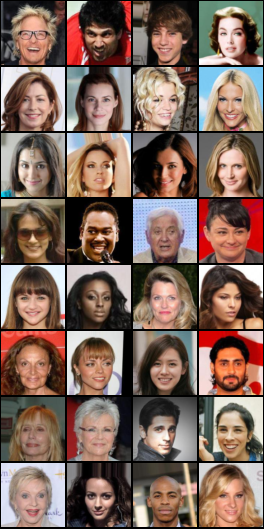
\includegraphics[width=\textwidth]{paper2/Images/celeba/vae_x_original.png}}%
      \label{fig:cvae_celeba_original_x}
  }
  \hfill
  \subfloat[$\bm{x}_u$ null-samples generated by the cVAE model.]{%
      \scalebox{0.3}{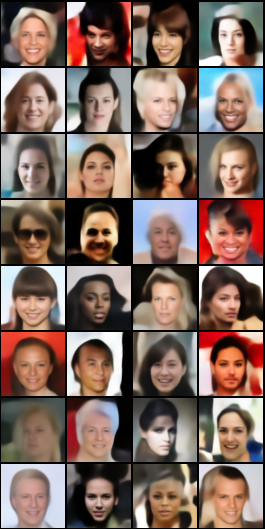
\includegraphics[width=\textwidth]{paper2/Images/celeba/vae_recon_y.png}}%
      \label{fig:cvae_celeba_recon_y}
  }
  \hfill
  \subfloat[$\bm{x}_b$ null-samples generated by the cVAE model.]{%
      \scalebox{0.3}{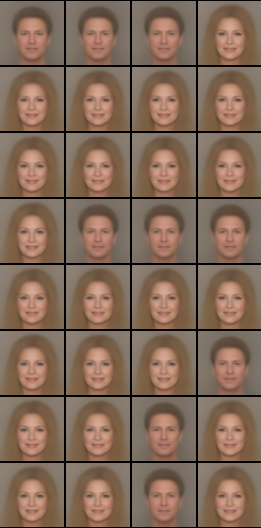
\includegraphics[width=\textwidth]{paper2/Images/celeba/vae_recon_s.png}}%
      \label{fig:cvae_celeba_recon_s}
  }
  \caption{
    CelebA null-samples learned by our cVAE model, with gender as the sensitive attribute.
    (a) The original, untransformed samples from the CelebA dataset
    (b) Reconstructions using only information unrelated to $s$.
    (c) Reconstruction using only information related to $\neg s$.
    The model learns to disentangle gender from the non-gender related information. Compared with the cFlow model, there is a severe degradation in reconstruction quality due to the model trying to simultaneously satisfy conflicting objectives.
    % Attributes such as \emph{makeup} and \emph{hair length} are also often modified in the process due to inherent correlations between them and the sensitive attribute, which the intepretability of our representations allows us to easily identify.
  }\label{fig:celeba_vae}
\end{figure*}

\begin{figure*}[tb]
  \centering
  \subfloat[Original images.]{%
      \scalebox{0.3}{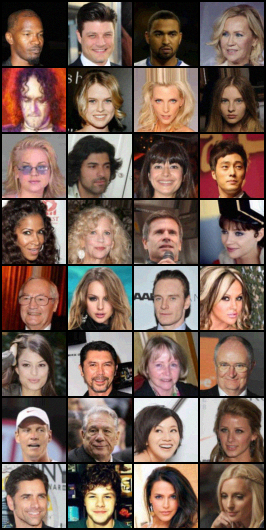
\includegraphics[width=\textwidth]{paper2/Images/celeba/cflow_original_x_suppmat.png}}%
      \label{fig:cflow_celeba_original_x_suppmat}
  }
  \hfill
  \subfloat[$\bm{x}_u$ null-samples generated by the cFlow model.]{%
      \scalebox{0.3}{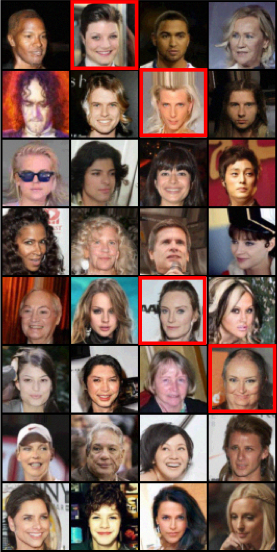
\includegraphics[width=\textwidth]{paper2/Images/celeba/cflow_xd_suppmat.png}}%
      \label{fig:cflow_celeba_recon_y_suppmt}
  }
  \hfill
  \subfloat[$\mathbf{x}_b$ null-samples generated by the cFlow model.]{%
      \scalebox{0.3}{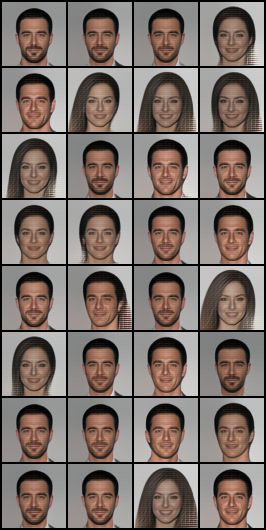
\includegraphics[width=\textwidth]{paper2/Images/celeba/cflow_xb_suppmat.png}}%
      \label{fig:cflow_celeba_recon_s_suppmat}
  }
  \caption{
    CelebA null-samples learned by our cFlow model, with gender as the sensitive attribute.
    (a) The original, untransformed samples from the CelebA dataset
    (b) Reconstructions using only information unrelated to $s$.
    (c) Reconstruction using only information related to $\neg s$.
    The model learns to disentangle gender from the non-gender related information.
    Attributes such as \emph{makeup} and \emph{hair length} are also often modified in the process (prime examples framed with red) due to inherent correlations between them and the sensitive attribute, which the interpretability of our representations allows us to easily identify.
  }\label{fig:celeba_cflow_suppmat}
\end{figure*}



\subsection{Transfer Learning}\label{sec:transfer-learning}
For our method, we require a representative set which follows the same distribution as that observed during deployment.
Such a representative set might not always be available.
In such a scenario, we can resort to using a set that is merely \emph{similar} to that in the deployment setting and leverage transfer learning.

%We argue that the inherent properties of INNs make them especially suitable for transfer learning.
One of the advantages of using an invertible architecture over conventional, \emph{surjective} ones that we stressed in the main text is its \emph{losslessness}. Since the transformations are necessarily bijective, the information contained in the input can never be destroyed, only redistributed. This makes such models particularly well-suited, in our minds, for transferring learned invariances:
even if the input is unfamiliar, no information should be lost when trying to transform it.
This works as long as only the information about $s$ ends up in the $z_b$ partition.
If $s$ takes a form similar to that which we pre-trained on, and can thus be correctly partitioned in the latent space, by complement we have the information about $\neg s$ stored in the $z_u$ partition, without presupposing similarity to the $\neg s$ observed during pre-training.

\paragraph{Transferring from mixed-NIST to MNIST.}
We test our hypothesis by comparing the performance of the cFlow and cVAE models pre-trained on a mixture of datasets belonging to the NIST family, colourised in the same way as cMNIST, while the downstream train and test sets remain the same as in the original cMNIST experiments. Specifically, we create this representative set by sampling 24,000 images (to match the cardinality of the original representative set) from EMNIST (letters only)~\citep{cohen2017emnist}, Fashion\-MNIST~\citep{xiao2017fashion} and KMNIST~\citep{clanuwat2018deep}, in equal proportion. We use the same architectures for the cVAE and cFlow models as we did in the non-transfer learning setting. In terms of hyperparameters, the only change made was to the KL-divergence's pre-factor, finding it necessary to increase it to $1$ to guarantee stability.

The results for the range of $\sigma$ values are shown in fig.~\ref{fig:cmnist-transfer}. Unsurprisingly, the performance of both models suffers when the representative and test sets do not completely correspond. However, the cFlow model consistently outperforms the cVAE model, with the gap increasing as the bias decreases.
Although some colour information is retained in the cFlow null-samples, symptomatic of an imperfect transfer, semantic information is almost entirely retained as well.
Conversely, the cVAE is very much flawed in this respect; as can be seen in the bottom row of fig.~\ref{fig:cmnist-transfer}, for some samples, semantic information is degraded to the point of the digit's identity being altered. As a result of this semantic degradation, the performance of the downstream classifier is curtailed by the noisiness of the digit's identity and is relatively unchanging across $\sigma$-values, in contrast to the monotonic improvement of that achieved on the cFlow null-samples.
% \begin{figure}
%   \includegraphics[width=0.6\textwidth]{paper2/Figures/nosinn_cmnist_transfer.pdf}
%   \caption{
%      Results for transfer learning experiments on cMNIST.
%   }%
%   \label{fig:cmnist-transfer}
% \end{figure}

\begin{figure*}[htb]
  \centering
  \subfloat[Performance on cMNIST test data after pre-training on the mixed NIST dataset.]{
      \scalebox{0.6}{\includegraphics[width=\textwidth]{paper2/Figures/nosinn_cmnist_transfer.pdf}} \label{fig:cmnist-transfer}
  }
  %---
  \vspace{10pt}
 
  \subfloat[Test data input to the cFlow model.]{%
      \scalebox{0.3}{\includegraphics[width=\textwidth]{paper2/Images/cmnist/cflow_tl_original.png}}%
      \label{fig:cflow_tl_original}
  }
  ~~~
%   \hfill
  \subfloat[$\bm{x}_u$ null-samples generated by the cFlow model.]{%
      \scalebox{0.3}{\includegraphics[width=\textwidth]{paper2/Images/cmnist/cflow_tl_xd.png}}%
      \label{fig:cflow_tl_xd}
  }
  
    \subfloat[Test data input to the cVAE model.]{%
      \scalebox{0.3}{\includegraphics[width=\textwidth]{paper2/Images/cmnist/cvae_tl_original.png}}%
      \label{fig:cvae_tl_original}
  }
  ~~~
%   \hfill
  \subfloat[$\bm{x}_u$ null-samples generated by the cVAE model.]{%
      \scalebox{0.3}{\includegraphics[width=\textwidth]{paper2/Images/cmnist/cvae_tl_xd.png}}%
      \label{fig:cvae_tl_xd}
  }
  \caption{
    Results for the transfer learning experiments in which the representative set consists of colourised samples from EMNIST, KMNIST, and FashionMNIST, while the downstream dataset remains as cMNIST. (a) Quantitative results for different $\sigma$-values. (b-c) Qualitative results for the cFlow model.
    (d-e) Qualitative results for the cVAE model. The qualitative results provide comparisons of the images before (left) and after (right) null-sampling. Note that for some of the cVAE samples, the clarity of the digits has clearly changed due to null-sampling, serving as an explanation for the non-increasing downstream performance.
  }%
  \label{fig:cmnist-transfer-all}
  
\end{figure*}

% \clearpage

% \bibliographystyle{splncs04}
% \bibliography{references.bib}

% \end{appendix}

% \end{document}

% \FloatBarrier%
% \clearpage

% \printbibliography%
% \end{refsection}

% \end{document}

\chapter{Paper 3: Learning with Perfect Bags: Addressing Hidden Stratification with Zero Labelled Data}\label{ch:paper3}
%%%%%%%%% ICML 2021 EXAMPLE LATEX SUBMISSION FILE %%%%%%%%%%%%%%%%%

%\documentclass{article}

%% Optional math commands from https://github.com/goodfeli/dlbook_notation.
%%%%%% NEW MATH DEFINITIONS %%%%%

\usepackage{amsmath,amsfonts,bm}

% Mark sections of captions for referring to divisions of figures
\newcommand{\figleft}{{\em (Left)}}
\newcommand{\figcenter}{{\em (Center)}}
\newcommand{\figright}{{\em (Right)}}
\newcommand{\figtop}{{\em (Top)}}
\newcommand{\figbottom}{{\em (Bottom)}}
\newcommand{\captiona}{{\em (a)}}
\newcommand{\captionb}{{\em (b)}}
\newcommand{\captionc}{{\em (c)}}
\newcommand{\captiond}{{\em (d)}}

% Highlight a newly defined term
\newcommand{\newterm}[1]{{\bf #1}}


% Figure reference, lower-case.
\def\figref#1{figure~\ref{#1}}
% Figure reference, capital. For start of sentence
\def\Figref#1{Figure~\ref{#1}}
\def\twofigref#1#2{figures \ref{#1} and \ref{#2}}
\def\quadfigref#1#2#3#4{figures \ref{#1}, \ref{#2}, \ref{#3} and \ref{#4}}
% Section reference, lower-case.
\def\secref#1{section~\ref{#1}}
% Section reference, capital.
\def\Secref#1{Section~\ref{#1}}
% Reference to two sections.
\def\twosecrefs#1#2{sections \ref{#1} and \ref{#2}}
% Reference to three sections.
\def\secrefs#1#2#3{sections \ref{#1}, \ref{#2} and \ref{#3}}
% Appendix reference, lower-case.
\def\appref#1{appendix~\ref{#1}}
% Appendix reference, capital.
\def\Appref#1{Appendix~\ref{#1}}
% Reference to an equation, lower-case.
\def\eqref#1{equation~\ref{#1}}
% Reference to an equation, upper case
\def\Eqref#1{Equation~\ref{#1}}
% A raw reference to an equation---avoid using if possible
\def\plaineqref#1{\ref{#1}}
% Reference to a chapter, lower-case.
\def\chapref#1{chapter~\ref{#1}}
% Reference to a Chapter, upper case.
\def\Chapref#1{Chapter~\ref{#1}}
\def\twochaprefs#1#2{chapters \ref{#1} and \ref{#2}}
% Reference to a range of chapters
\def\rangechapref#1#2{chapters \ref{#1}--\ref{#2}}
% Reference to a range of chapters, upper case
\def\Rangechapref#1#2{Chapters \ref{#1}--\ref{#2}}
% Reference to an algorithm, lower-case.
\def\algref#1{algorithm~\ref{#1}}
% Reference to an algorithm, upper case.
\def\Algref#1{Algorithm~\ref{#1}}
\def\twoalgref#1#2{algorithms \ref{#1} and \ref{#2}}
\def\Twoalgref#1#2{Algorithms \ref{#1} and \ref{#2}}
% Reference to a part, lower case
\def\partref#1{part~\ref{#1}}
% Reference to a part, upper case
\def\Partref#1{Part~\ref{#1}}
\def\twopartref#1#2{parts \ref{#1} and \ref{#2}}

\def\ceil#1{\lceil #1 \rceil}
\def\floor#1{\lfloor #1 \rfloor}
\def\1{\bm{1}}
\newcommand{\train}{\mathcal{D}}
\newcommand{\valid}{\mathcal{D_{\mathrm{valid}}}}
\newcommand{\test}{\mathcal{D_{\mathrm{test}}}}

\def\eps{{\epsilon}}


% Random variables
\def\reta{{\textnormal{$\eta$}}}
\def\ra{{\textnormal{a}}}
\def\rb{{\textnormal{b}}}
\def\rc{{\textnormal{c}}}
\def\rd{{\textnormal{d}}}
\def\re{{\textnormal{e}}}
\def\rf{{\textnormal{f}}}
\def\rg{{\textnormal{g}}}
\def\rh{{\textnormal{h}}}
\def\ri{{\textnormal{i}}}
\def\rj{{\textnormal{j}}}
\def\rk{{\textnormal{k}}}
\def\rl{{\textnormal{l}}}
% rm is already a command, just don't name any random variables m
\def\rn{{\textnormal{n}}}
\def\ro{{\textnormal{o}}}
\def\rp{{\textnormal{p}}}
\def\rq{{\textnormal{q}}}
\def\rr{{\textnormal{r}}}
\def\rs{{\textnormal{s}}}
\def\rt{{\textnormal{t}}}
\def\ru{{\textnormal{u}}}
\def\rv{{\textnormal{v}}}
\def\rw{{\textnormal{w}}}
\def\rx{{\textnormal{x}}}
\def\ry{{\textnormal{y}}}
\def\rz{{\textnormal{z}}}

% Random vectors
\def\rvepsilon{{\mathbf{\epsilon}}}
\def\rvtheta{{\mathbf{\theta}}}
\def\rva{{\mathbf{a}}}
\def\rvb{{\mathbf{b}}}
\def\rvc{{\mathbf{c}}}
\def\rvd{{\mathbf{d}}}
\def\rve{{\mathbf{e}}}
\def\rvf{{\mathbf{f}}}
\def\rvg{{\mathbf{g}}}
\def\rvh{{\mathbf{h}}}
\def\rvu{{\mathbf{i}}}
\def\rvj{{\mathbf{j}}}
\def\rvk{{\mathbf{k}}}
\def\rvl{{\mathbf{l}}}
\def\rvm{{\mathbf{m}}}
\def\rvn{{\mathbf{n}}}
\def\rvo{{\mathbf{o}}}
\def\rvp{{\mathbf{p}}}
\def\rvq{{\mathbf{q}}}
\def\rvr{{\mathbf{r}}}
\def\rvs{{\mathbf{s}}}
\def\rvt{{\mathbf{t}}}
\def\rvu{{\mathbf{u}}}
\def\rvv{{\mathbf{v}}}
\def\rvw{{\mathbf{w}}}
\def\rvx{{\mathbf{x}}}
\def\rvy{{\mathbf{y}}}
\def\rvz{{\mathbf{z}}}

% Elements of random vectors
\def\erva{{\textnormal{a}}}
\def\ervb{{\textnormal{b}}}
\def\ervc{{\textnormal{c}}}
\def\ervd{{\textnormal{d}}}
\def\erve{{\textnormal{e}}}
\def\ervf{{\textnormal{f}}}
\def\ervg{{\textnormal{g}}}
\def\ervh{{\textnormal{h}}}
\def\ervi{{\textnormal{i}}}
\def\ervj{{\textnormal{j}}}
\def\ervk{{\textnormal{k}}}
\def\ervl{{\textnormal{l}}}
\def\ervm{{\textnormal{m}}}
\def\ervn{{\textnormal{n}}}
\def\ervo{{\textnormal{o}}}
\def\ervp{{\textnormal{p}}}
\def\ervq{{\textnormal{q}}}
\def\ervr{{\textnormal{r}}}
\def\ervs{{\textnormal{s}}}
\def\ervt{{\textnormal{t}}}
\def\ervu{{\textnormal{u}}}
\def\ervv{{\textnormal{v}}}
\def\ervw{{\textnormal{w}}}
\def\ervx{{\textnormal{x}}}
\def\ervy{{\textnormal{y}}}
\def\ervz{{\textnormal{z}}}

% Random matrices
\def\rmA{{\mathbf{A}}}
\def\rmB{{\mathbf{B}}}
\def\rmC{{\mathbf{C}}}
\def\rmD{{\mathbf{D}}}
\def\rmE{{\mathbf{E}}}
\def\rmF{{\mathbf{F}}}
\def\rmG{{\mathbf{G}}}
\def\rmH{{\mathbf{H}}}
\def\rmI{{\mathbf{I}}}
\def\rmJ{{\mathbf{J}}}
\def\rmK{{\mathbf{K}}}
\def\rmL{{\mathbf{L}}}
\def\rmM{{\mathbf{M}}}
\def\rmN{{\mathbf{N}}}
\def\rmO{{\mathbf{O}}}
\def\rmP{{\mathbf{P}}}
\def\rmQ{{\mathbf{Q}}}
\def\rmR{{\mathbf{R}}}
\def\rmS{{\mathbf{S}}}
\def\rmT{{\mathbf{T}}}
\def\rmU{{\mathbf{U}}}
\def\rmV{{\mathbf{V}}}
\def\rmW{{\mathbf{W}}}
\def\rmX{{\mathbf{X}}}
\def\rmY{{\mathbf{Y}}}
\def\rmZ{{\mathbf{Z}}}

% Elements of random matrices
\def\ermA{{\textnormal{A}}}
\def\ermB{{\textnormal{B}}}
\def\ermC{{\textnormal{C}}}
\def\ermD{{\textnormal{D}}}
\def\ermE{{\textnormal{E}}}
\def\ermF{{\textnormal{F}}}
\def\ermG{{\textnormal{G}}}
\def\ermH{{\textnormal{H}}}
\def\ermI{{\textnormal{I}}}
\def\ermJ{{\textnormal{J}}}
\def\ermK{{\textnormal{K}}}
\def\ermL{{\textnormal{L}}}
\def\ermM{{\textnormal{M}}}
\def\ermN{{\textnormal{N}}}
\def\ermO{{\textnormal{O}}}
\def\ermP{{\textnormal{P}}}
\def\ermQ{{\textnormal{Q}}}
\def\ermR{{\textnormal{R}}}
\def\ermS{{\textnormal{S}}}
\def\ermT{{\textnormal{T}}}
\def\ermU{{\textnormal{U}}}
\def\ermV{{\textnormal{V}}}
\def\ermW{{\textnormal{W}}}
\def\ermX{{\textnormal{X}}}
\def\ermY{{\textnormal{Y}}}
\def\ermZ{{\textnormal{Z}}}

% Vectors
\def\vzero{{\bm{0}}}
\def\vone{{\bm{1}}}
\def\vmu{{\bm{\mu}}}
\def\vtheta{{\bm{\theta}}}
\def\va{{\bm{a}}}
\def\vb{{\bm{b}}}
\def\vc{{\bm{c}}}
\def\vd{{\bm{d}}}
\def\ve{{\bm{e}}}
\def\vf{{\bm{f}}}
\def\vg{{\bm{g}}}
\def\vh{{\bm{h}}}
\def\vi{{\bm{i}}}
\def\vj{{\bm{j}}}
\def\vk{{\bm{k}}}
\def\vl{{\bm{l}}}
\def\vm{{\bm{m}}}
\def\vn{{\bm{n}}}
\def\vo{{\bm{o}}}
\def\vp{{\bm{p}}}
\def\vq{{\bm{q}}}
\def\vr{{\bm{r}}}
\def\vs{{\bm{s}}}
\def\vt{{\bm{t}}}
\def\vu{{\bm{u}}}
\def\vv{{\bm{v}}}
\def\vw{{\bm{w}}}
\def\vx{{\bm{x}}}
\def\vy{{\bm{y}}}
\def\vz{{\bm{z}}}

% Elements of vectors
\def\evalpha{{\alpha}}
\def\evbeta{{\beta}}
\def\evepsilon{{\epsilon}}
\def\evlambda{{\lambda}}
\def\evomega{{\omega}}
\def\evmu{{\mu}}
\def\evpsi{{\psi}}
\def\evsigma{{\sigma}}
\def\evtheta{{\theta}}
\def\eva{{a}}
\def\evb{{b}}
\def\evc{{c}}
\def\evd{{d}}
\def\eve{{e}}
\def\evf{{f}}
\def\evg{{g}}
\def\evh{{h}}
\def\evi{{i}}
\def\evj{{j}}
\def\evk{{k}}
\def\evl{{l}}
\def\evm{{m}}
\def\evn{{n}}
\def\evo{{o}}
\def\evp{{p}}
\def\evq{{q}}
\def\evr{{r}}
\def\evs{{s}}
\def\evt{{t}}
\def\evu{{u}}
\def\evv{{v}}
\def\evw{{w}}
\def\evx{{x}}
\def\evy{{y}}
\def\evz{{z}}

% Matrix
\def\mA{{\bm{A}}}
\def\mB{{\bm{B}}}
\def\mC{{\bm{C}}}
\def\mD{{\bm{D}}}
\def\mE{{\bm{E}}}
\def\mF{{\bm{F}}}
\def\mG{{\bm{G}}}
\def\mH{{\bm{H}}}
\def\mI{{\bm{I}}}
\def\mJ{{\bm{J}}}
\def\mK{{\bm{K}}}
\def\mL{{\bm{L}}}
\def\mM{{\bm{M}}}
\def\mN{{\bm{N}}}
\def\mO{{\bm{O}}}
\def\mP{{\bm{P}}}
\def\mQ{{\bm{Q}}}
\def\mR{{\bm{R}}}
\def\mS{{\bm{S}}}
\def\mT{{\bm{T}}}
\def\mU{{\bm{U}}}
\def\mV{{\bm{V}}}
\def\mW{{\bm{W}}}
\def\mX{{\bm{X}}}
\def\mY{{\bm{Y}}}
\def\mZ{{\bm{Z}}}
\def\mBeta{{\bm{\beta}}}
\def\mPhi{{\bm{\Phi}}}
\def\mLambda{{\bm{\Lambda}}}
\def\mSigma{{\bm{\Sigma}}}

% % Tensor
% \DeclareMathAlphabet{\mathsfit}{\encodingdefault}{\sfdefault}{m}{sl}
% \SetMathAlphabet{\mathsfit}{bold}{\encodingdefault}{\sfdefault}{bx}{n}
% \newcommand{\tens}[1]{\bm{\mathsfit{#1}}}
% \def\tA{{\tens{A}}}
% \def\tB{{\tens{B}}}
% \def\tC{{\tens{C}}}
% \def\tD{{\tens{D}}}
% \def\tE{{\tens{E}}}
% \def\tF{{\tens{F}}}
% \def\tG{{\tens{G}}}
% \def\tH{{\tens{H}}}
% \def\tI{{\tens{I}}}
% \def\tJ{{\tens{J}}}
% \def\tK{{\tens{K}}}
% \def\tL{{\tens{L}}}
% \def\tM{{\tens{M}}}
% \def\tN{{\tens{N}}}
% \def\tO{{\tens{O}}}
% \def\tP{{\tens{P}}}
% \def\tQ{{\tens{Q}}}
% \def\tR{{\tens{R}}}
% \def\tS{{\tens{S}}}
% \def\tT{{\tens{T}}}
% \def\tU{{\tens{U}}}
% \def\tV{{\tens{V}}}
% \def\tW{{\tens{W}}}
% \def\tX{{\tens{X}}}
% \def\tY{{\tens{Y}}}
% \def\tZ{{\tens{Z}}}


% Graph
\def\gA{{\mathcal{A}}}
\def\gB{{\mathcal{B}}}
\def\gC{{\mathcal{C}}}
\def\gD{{\mathcal{D}}}
\def\gE{{\mathcal{E}}}
\def\gF{{\mathcal{F}}}
\def\gG{{\mathcal{G}}}
\def\gH{{\mathcal{H}}}
\def\gI{{\mathcal{I}}}
\def\gJ{{\mathcal{J}}}
\def\gK{{\mathcal{K}}}
\def\gL{{\mathcal{L}}}
\def\gM{{\mathcal{M}}}
\def\gN{{\mathcal{N}}}
\def\gO{{\mathcal{O}}}
\def\gP{{\mathcal{P}}}
\def\gQ{{\mathcal{Q}}}
\def\gR{{\mathcal{R}}}
\def\gS{{\mathcal{S}}}
\def\gT{{\mathcal{T}}}
\def\gU{{\mathcal{U}}}
\def\gV{{\mathcal{V}}}
\def\gW{{\mathcal{W}}}
\def\gX{{\mathcal{X}}}
\def\gY{{\mathcal{Y}}}
\def\gZ{{\mathcal{Z}}}

% Sets
\def\sA{{\mathbb{A}}}
\def\sB{{\mathbb{B}}}
\def\sC{{\mathbb{C}}}
\def\sD{{\mathbb{D}}}
% Don't use a set called E, because this would be the same as our symbol
% for expectation.
\def\sF{{\mathbb{F}}}
\def\sG{{\mathbb{G}}}
\def\sH{{\mathbb{H}}}
\def\sI{{\mathbb{I}}}
\def\sJ{{\mathbb{J}}}
\def\sK{{\mathbb{K}}}
\def\sL{{\mathbb{L}}}
\def\sM{{\mathbb{M}}}
\def\sN{{\mathbb{N}}}
\def\sO{{\mathbb{O}}}
\def\sP{{\mathbb{P}}}
\def\sQ{{\mathbb{Q}}}
\def\sR{{\mathbb{R}}}
\def\sS{{\mathbb{S}}}
\def\sT{{\mathbb{T}}}
\def\sU{{\mathbb{U}}}
\def\sV{{\mathbb{V}}}
\def\sW{{\mathbb{W}}}
\def\sX{{\mathbb{X}}}
\def\sY{{\mathbb{Y}}}
\def\sZ{{\mathbb{Z}}}

% Entries of a matrix
\def\emLambda{{\Lambda}}
\def\emA{{A}}
\def\emB{{B}}
\def\emC{{C}}
\def\emD{{D}}
\def\emE{{E}}
\def\emF{{F}}
\def\emG{{G}}
\def\emH{{H}}
\def\emI{{I}}
\def\emJ{{J}}
\def\emK{{K}}
\def\emL{{L}}
\def\emM{{M}}
\def\emN{{N}}
\def\emO{{O}}
\def\emP{{P}}
\def\emQ{{Q}}
\def\emR{{R}}
\def\emS{{S}}
\def\emT{{T}}
\def\emU{{U}}
\def\emV{{V}}
\def\emW{{W}}
\def\emX{{X}}
\def\emY{{Y}}
\def\emZ{{Z}}
\def\emSigma{{\Sigma}}

% entries of a tensor
% Same font as tensor, without \bm wrapper
% \newcommand{\etens}[1]{\mathsfit{#1}}
% \def\etLambda{{\etens{\Lambda}}}
% \def\etA{{\etens{A}}}
% \def\etB{{\etens{B}}}
% \def\etC{{\etens{C}}}
% \def\etD{{\etens{D}}}
% \def\etE{{\etens{E}}}
% \def\etF{{\etens{F}}}
% \def\etG{{\etens{G}}}
% \def\etH{{\etens{H}}}
% \def\etI{{\etens{I}}}
% \def\etJ{{\etens{J}}}
% \def\etK{{\etens{K}}}
% \def\etL{{\etens{L}}}
% \def\etM{{\etens{M}}}
% \def\etN{{\etens{N}}}
% \def\etO{{\etens{O}}}
% \def\etP{{\etens{P}}}
% \def\etQ{{\etens{Q}}}
% \def\etR{{\etens{R}}}
% \def\etS{{\etens{S}}}
% \def\etT{{\etens{T}}}
% \def\etU{{\etens{U}}}
% \def\etV{{\etens{V}}}
% \def\etW{{\etens{W}}}
% \def\etX{{\etens{X}}}
% \def\etY{{\etens{Y}}}
% \def\etZ{{\etens{Z}}}

% The true underlying data generating distribution
\newcommand{\pdata}{p_{\rm{data}}}
% The empirical distribution defined by the training set
\newcommand{\ptrain}{\hat{p}_{\rm{data}}}
\newcommand{\Ptrain}{\hat{P}_{\rm{data}}}
% The model distribution
\newcommand{\pmodel}{p_{\rm{model}}}
\newcommand{\Pmodel}{P_{\rm{model}}}
\newcommand{\ptildemodel}{\tilde{p}_{\rm{model}}}
% Stochastic autoencoder distributions
\newcommand{\pencode}{p_{\rm{encoder}}}
\newcommand{\pdecode}{p_{\rm{decoder}}}
\newcommand{\precons}{p_{\rm{reconstruct}}}

\newcommand{\laplace}{\mathrm{Laplace}} % Laplace distribution

\newcommand{\E}{\mathbb{E}}
\newcommand{\Ls}{\mathcal{L}}
\newcommand{\R}{\mathbb{R}}
\newcommand{\emp}{\tilde{p}}
\newcommand{\lr}{\alpha}
\newcommand{\reg}{\lambda}
\newcommand{\rect}{\mathrm{rectifier}}
\newcommand{\softmax}{\mathrm{softmax}}
\newcommand{\sigmoid}{\sigma}
\newcommand{\softplus}{\zeta}
\newcommand{\KL}{D_{\mathrm{KL}}}
\newcommand{\Var}{\mathrm{Var}}
\newcommand{\standarderror}{\mathrm{SE}}
\newcommand{\Cov}{\mathrm{Cov}}
% Wolfram Mathworld says $L^2$ is for function spaces and $\ell^2$ is for vectors
% But then they seem to use $L^2$ for vectors throughout the site, and so does
% wikipedia.
\newcommand{\normlzero}{L^0}
\newcommand{\normlone}{L^1}
\newcommand{\normltwo}{L^2}
\newcommand{\normlp}{L^p}
\newcommand{\normmax}{L^\infty}

\newcommand{\parents}{Pa} % See usage in notation.tex. Chosen to match Daphne's book.

\DeclareMathOperator*{\argmax}{arg\,max}
\DeclareMathOperator*{\argmin}{arg\,min}

\DeclareMathOperator{\sign}{sign}
\DeclareMathOperator{\Tr}{Tr}
\let\ab\allowbreak


%% Recommended, but optional, packages for figures and better typesetting:
%\usepackage{microtype}
%\usepackage{graphicx}
%\usepackage{wrapfig}
%\usepackage{caption}
%\usepackage{subcaption}
%\usepackage{booktabs} % for professional tables
%\usepackage{amsfonts}       % blackboard math symbols
%\usepackage{amsmath}
%\usepackage{amssymb}
%\usepackage{amsthm}
%\usepackage{nicefrac}       % compact symbols for 1/2, etc.
%\usepackage{xcolor}         %for colouring the text on colourMNIST
%\usepackage{comment}
%\usepackage{enumitem}
%\newtheorem{prop}{Proposition}
%\newcommand{\Xcal}{\mathcal{X}}
%\newcommand{\Bcal}{\mathcal{B}}
%\newcommand{\Ycal}{\mathcal{Y}}
%\newcommand{\Scal}{\mathcal{S}}
%\newcommand{\Lcal}{\mathcal{L}}
%\newcommand{\Dcal}{\mathcal{D}}
%\newcommand{\ie}{i.\,e.}
%\newcommand{\Ie}{I.\,e.}
%\newcommand{\eg}{e.\,g.}
%\newcommand{\Eg}{E.\,g.}

%% hyperref makes hyperlinks in the resulting PDF.
%% If your build breaks (sometimes temporarily if a hyperlink spans a page)
%% please comment out the following usepackage line and replace
%% \usepackage{icml2021} with \usepackage[nohyperref]{icml2021} above.
%\usepackage{hyperref}

%% Attempt to make hyperref and algorithmic work together better:
%\newcommand{\theHalgorithm}{\arabic{algorithm}}

%% Use the following line for the initial blind version submitted for review:
%\usepackage{icml2021}

%% If accepted, instead use the following line for the camera-ready submission:
%%\usepackage[accepted]{icml2021}

%% The \icmltitle you define below is probably too long as a header.
%% Therefore, a short form for the running title is supplied here:
%\icmltitlerunning{Learning with Perfect Bags}

%\begin{document}

%\twocolumn[
%\icmltitle{Learning with Perfect Bags:\\
%Addressing Hidden Stratification with Zero Labelled Data}

%% It is OKAY to include author information, even for blind
%% submissions: the style file will automatically remove it for you
%% unless you've provided the [accepted] option to the icml2021
%% package.

%% List of affiliations: The first argument should be a (short)
%% identifier you will use later to specify author affiliations
%% Academic affiliations should list Department, University, City, Region, Country
%% Industry affiliations should list Company, City, Region, Country

%% You can specify symbols, otherwise they are numbered in order.
%% Ideally, you should not use this facility. Affiliations will be numbered
%% in order of appearance and this is the preferred way.
%\icmlsetsymbol{equal}{*}

%\begin{icmlauthorlist}
%\icmlauthor{Aeiau Zzzz}{equal,to}
%\icmlauthor{Bauiu C.~Yyyy}{equal,to,goo}
%\icmlauthor{Cieua Vvvvv}{goo}
%\icmlauthor{Iaesut Saoeu}{ed}
%\icmlauthor{Fiuea Rrrr}{to}
%\icmlauthor{Tateu H.~Yasehe}{ed,to,goo}
%\icmlauthor{Aaoeu Iasoh}{goo}
%\icmlauthor{Buiui Eueu}{ed}
%\icmlauthor{Aeuia Zzzz}{ed}
%\icmlauthor{Bieea C.~Yyyy}{to,goo}
%\icmlauthor{Teoau Xxxx}{ed}
%\icmlauthor{Eee Pppp}{ed}
%\end{icmlauthorlist}

%\icmlaffiliation{to}{Department of Computation, University of Torontoland, Torontoland, Canada}
%\icmlaffiliation{goo}{Googol ShallowMind, New London, Michigan, USA}
%\icmlaffiliation{ed}{School of Computation, University of Edenborrow, Edenborrow, United Kingdom}

%\icmlcorrespondingauthor{Cieua Vvvvv}{c.vvvvv@googol.com}
%\icmlcorrespondingauthor{Eee Pppp}{ep@eden.co.uk}

%% You may provide any keywords that you
%% find helpful for describing your paper; these are used to populate
%% the "keywords" metadata in the PDF but will not be shown in the document
%\icmlkeywords{semi-supervised learning, dataset bias}

%\vskip 0.3in
%]

%% this must go after the closing bracket ] following \twocolumn[ ...

%% This command actually creates the footnote in the first column
%% listing the affiliations and the copyright notice.
%% The command takes one argument, which is text to display at the start of the footnote.
%% The \icmlEqualContribution command is standard text for equal contribution.
%% Remove it (just {}) if you do not need this facility.

%%\printAffiliationsAndNotice{}  % leave blank if no need to mention equal contribution
%\printAffiliationsAndNotice{\icmlEqualContribution} % otherwise use the standard text.

%\icmltitle{Learning with Perfect Bags:\\
%Addressing Hidden Stratification with Zero Labelled Data}
\textsc{Authors}:\\
Thomas Kehrenberg$^1$, Viktoriia Sharmanska$^1$, Myles Bartlett$^1$, and Novi Quadrianto$^1$ \\
\textsc{Affiliations}:\\
$^1$ Predictive Analytics Lab (PAL), University of Sussex, Brighton, UK\\
\textsc{Conference}:\;\; Submitted to \textit{International Conference on Machine Learning} (ICML), 2021 \\
% \textsc{DOI}:\;\;10.3389/frai.2020.00033
\textsc{Note}:\;\; The appendix has been included as section~\ref{sec:zsf-appendix}.

\section{Abstract}
Machine learning models are typically trained to optimise global metrics such as average classification accuracy. 
%
Hidden stratification arises when the trained models have high average performance over classes but exhibit highly variable performance across different hidden subgroups.
%
In this paper, we consider the setting where the hidden stratification has zero class-labelled data for some subgroups. 
As an illustration, we have digit images labelled as "two" or "four", each class comprises "green" and "purple" subgroups.
%
Challengingly, in the training data, twos can be any colour, but all fours are green. 
%
Without additional knowledge, it is impossible to directly control the discrepancy of the classifier’s statistics for the hidden subgroups. 
%
We develop a disentanglement algorithm that decomposes a data representation into a component that captures the subgrouping factors and a component that is invariant to them based on unlabelled (deployment) data. 
%
We cluster the unlabelled data, and equalise the cluster sizes to form "perfect bags" with respect to class and subgroup information.
%
We cast the problem of disentangling as one of distribution matching and propose an adversarial learning approach.
%
%We introduce a new discriminator loss, inspired by set-classification, to distinguish a batch of perfect bags from non-perfect ones based on a learnable attention mechanism. 
%
Unlike sample-based models, we advance a discriminator to assign scores at the level of bags of samples, with a bag being deemed authentic if was drawn from the unbiased distribution. 
%a parametric approach based on adversarial learning. 
%We take inspiration from set-classification and equip the discriminator with a learnable attention mechanism to model interdependencies between samples in a bag.
%
We evaluate our approach on several classification benchmarks and show that it is indeed possible to account for zero-label hidden stratification.
% \end{abstract}

\section{Introduction}%
\label{sec:introduction}
Machine learning has been deployed in safety-critical applications such as medicine (e.g. \citep{DunYiLanReetal19}), and socially important contexts such as the allocation of healthcare, education, and credit (\eg\ \citep{HurAde17,RagBarKleLev20}). 
%
Efficiency can be improved, costs can be reduced, and personalisation of services and products can be greatly enhanced -- these are some of the drivers for the widespread development and deployment of machine learning algorithms. 
%

Algorithms such as classifiers, however, are trained from large amount of labelled data, and are typically trained to optimise \emph{global} metrics such as average classification accuracy.
%
% \begin{figure*}[t]
% \centering
% \includegraphics[width=0.6\textwidth,page=2]{paper3/figures/ideal.pdf}
% \caption{Overview of the zero-shot stratification problem. Training dataset (pairs of input data $x$ and class label $y$) will only contain data points that are labelled ``yes'' by the decision policy. This systematic bias might result in a subgroup(s) to have zero labelled data (in the example above, ``married'' subgroup has zero labelled data). The subgrouping information $s$ is unavailable/unlabelled at deployment time, and is only partially labelled at train time.}
% \vspace{-0.5cm}
% \label{fig:censoring}
% \end{figure*}
In many real-world classification tasks, each labelled class consists of multiple semantically distinct subclasses, or subgroups.
For example, the ``dog'' class label can have finer-grained intra-class variations, such as ``dog indoor'' and ``dog outdoor''.
%
This finer-grained subgrouping information is typically unavailable/unlabelled (e.g. \citep{SohDunAngGuetal20,nam2020learning}).
%
The standard training process brings about two inter-connected challenges: a) classifiers often under-perform on important hidden subgroups (\emph{hidden stratification}) \citep{RayDunCarRe20,SohDunAngGuetal20};
and b) \emph{systematic bias}~\citep{kallus2018residual} affects whether or not entire collections of data points appear in the training dataset,
and can make the classifier unprepared for treating those subgroups in the eventual deployment setting
% and can hamper attempts to correct for bias in the eventual deployment data
(\emph{residual bias}). %\cite{kallus2018residual}.

We are interested in hidden stratification in which, for some of the subgroups, labelled training data is only available with a certain outcome, or labelled training samples are not available at all, due to systematic bias.
This can be seen as a strong sampling bias.
%
For instance, data on loan defaults can only be collected on those loan
applicants who were approved in the past \citep{kallus2018residual}.
%
Here a loan decision policy specifies whether an individual will be included in the training dataset.
%
Individuals can be thought of as belonging to a specific subgroup such as ``married'' or ``not married'' and systematic bias produced by a historical decision policy may result in the ``not married'' subgroup having poor, or altogether non-existent, representation.
%For instance, a medical imaging model trained to classify between ``benign'' and ``abnormal'' lesions may achieve high overall performance, yet consistently mislabel a rare but critical abnormal subgroup as ``benign'' \cite{DunYiLanReetal19}.
%
%Each class actually composes of ``no-patch'' and ``patch'' hidden subgroups, and the ``no-patch'' subgroup is further splitted into “histopathology” and “non-histopathology”.
%
%A past decision policy of \emph{not} requiring histopathology (biopsy \& pathologist referral) specifies whether an individual will be included in the training dataset.
%
%This systematic bias might lead to the no-patch subgroup to have thin or non-existent labelled data.
%
We formalise this stratification problem as a data setting where a decision policy can lead to one or more subgroups having no labelled data.

To address the problem of subgroup bias, this paper focuses on learning subgroup-invariant representations in the presence of zero-label stratification.
These representations can then be used to train a classifier that generalises to the deployment setting which does not exhibit the bias of the training set.
%
To learn the representation, a form of supervision is needed.
Our source of supervision is motivated by the observation that we want to deploy our classifier to the eventual real-world population.
%
A deployment set will contain data points from all subgroups.
%
We thus consider the setting where \emph{unlabelled} data is available for learning representations that disentangle the subgroup membership from the class membership. We note, however, that the test set could be used for this purpose in a transductive setting.

We aim to convert our unlabelled data into a collection of \emph{perfect bags} \citep{kleinberg2016inherent,chouldechova2017fair}, \ie\ sample sets in which the class label $y$ and subgroup label $s$ are independent (\ie\ $y\perp s$).
Making use of the terminology from \emph{multiple-instance learning}, our batches comprise a certain number of bags which are a collection of samples.
%
We will then use these perfect bags as the inductive bias for learning the disentangled representations. 
%
How can we construct these perfect bags in the absence of any labelled data?
%
We assume that the number of subgroups is known \emph{a priori}\footnote{Relaxing this assumption represents a clear avenue for future work. We elaborate this in the limitation and intended use sec.~\ref{sec:limitations}.}. 
%We elaborate this further in our experiments and discussions sections.}.
%corresponding to the diverse demographic groups in the real-world population in which our machine learning system will be deployed. 
%
We then apply unsupervised k-means clustering, or a \emph{semi}-supervised clustering based on rank statistics; the latter allows incorporating annotations from the training data when forming the clusters.
%
Once the clusters have been found, we can sample from each cluster at an equal rate to form balanced (\ie\,\emph{perfect}) bags and use them as input for learning a disentangled representation. 
%
%See fig. \ref{fig:teaser} for an overview of our learning with invisible demographic framework.
We cast the problem of disentangling as one of distribution matching and propose an adversarial learning approach.
%a parametric approach based on adversarial learning. 
In the standard GAN setting, the discriminator assigns a score to each sample corresponding to the perceived probability that it was drawn from the true data distribution, and not the generator's.
In contrast, we train a discriminator to assign scores at the level of bags of samples, with a bag being deemed authentic if it was drawn from the originally unbiased distribution and not the de-biased one (with the de-biaser playing the role of the generator). To do so, we take inspiration from set-classification and multiple-instance learning and equip the discriminator with a learnable attention mechanism to model interdependencies between samples in a bag.

Specifically, our paper provides the following contributions:
\begin{enumerate}
    \item An example of systematic bias leading to one or more  subgroups having \emph{zero labelled data}.
    \item Applying clustering methods to the task of transforming an \emph{unlabelled dataset} into perfect bags.
    \item Theoretical and experimental justification that the disentangling model with \emph{the perfect bag as an inductive bias} provides a well-disentangled representation, where one component captures the subgrouping factors and another component is invariant to them.
    \item A new parametric approach to disentangling that combines elements from adversarial learning and set-classification to guide an encoder network towards the goal of producing encodings invariant to the source distribution and thereby the subgroup factors in which source distributions differ.
\end{enumerate}

\section{Related work.}
We describe related work in two areas: zero-shot learning and semi-su\-per\-vi\-sed learning.
%and disentangled representation learning. 

\subsection{On zero-shot learning.}
The setting with incomplete training data, where we aim to account for seen and unseen outcomes is also known as \emph{generalised zero-shot learning}. 
Traditionally, zero-shot learning transfers knowledge from classes for which we have training data to classes for which we do not, via auxiliary knowledge, e.g. via prototype examples \citep{larochelle2008}, intermediate class description such as semantic attributes \citep{lampert2009, xian2018zero}, word2vec embeddings \citep{bucher2019}. 
Our method similarly uses a collection of perfect bags as a source of auxiliary knowledge but in contrast to generalised zero-shot learning, our perfect bag is an unlabelled pool of data, where class descriptions are unknown. 

\subsection{On semi-supervised learning.} 
\citet{wick2019unlocking} proposed a semi-supervised method that can successfully harness unlabelled data to correct for the selection bias and label bias in the training data.
%
The unlabelled data, despite not containing the class label $y$, \emph{is} labelled in terms of the subgroup label $s$. 
%
Our setting is significantly harder because there is no label information about $y$ and $s$ in the perfect bag.

\subsection{On disentangled representations learning.}
\citet{locatello2019fairness} suggested that disentanglement in representation learning may be a useful property to remove algorithmic bias when subgroup information is not observed.
%
In order for disentangled representations to reduce algorithmic bias without the knowledge of subgroup label $s$, they have to assume that the class label $y$ and the subgroup label $s$ are independent, i.e. $y\perp s$.
%
Though, in many real-world tasks, the variable $s$ is correlated with the variable $y$, and therefore unsupervised methods are not suitable  \citep{jaiswal2018unsupervised,JaiWuAbdNat19}. 
%
Indeed, experiments in \citet{locatello2019fairness} were wholly done with procedurally generated synthetic datasets involving 2D and 3D shapes. 
%
Without some supervision or inductive bias, disentangled representation methods would not solve the issue of algorithmic fairness with invisible demographics \citep{locatello2019challenging}. 

%\begin{wrapfigure}{!t}{0.6\textwidth}
\begin{figure}[t]
\centering
    %\includegraphics[width=0.9\textwidth]{paper3/figures/SSL-framework}
    % \includegraphics[width=\textwidth]{paper3/figures/SSL-framework-withPred.pdf}
    \includegraphics[width=\textwidth]{paper3/figures/zsf_diagram.pdf}
    \caption{%
    The main components involved in our proposed disentangling method, $f_y$ (debiaser) and $h$ (discriminator). The debiaser is trained to produce encodings, $z_y$ of the data that are invariant to the source dataset and thereby the subgroups identifying it. In order to determine whether a bag of encodings originates from the training set or the deployment set, the discriminator performs an attention-weighted aggregation over the bag dimension to model interdependencies between the samples. In the case of Coloured MNIST where {\color{purple}purple} fours constitute the missing subgroup, the discriminator can identify an encoding of a bag from the training set by the absence of such samples so long as colour information is detectable in $z_y$, serving as an error signal for the debiaser.
    }%
    \label{fig:architecture}
\end{figure}%
% \end{figure}
%\end{wrapfigure}
% \hfill
% \begin{figure}
\begin{figure}[t]
    \centering
    % if you want to make changes to the diagram, it is located here:
    % https://drive.google.com/file/d/1M37m4rVj1EGrFJb9QzK32bs8swepiaZ1/view?usp=sharing
    \includegraphics[width=0.5\textwidth]{paper3/figures/fdm.pdf}
    \caption{%
    Illustration of distribution matching.
    In this example, the training set is lacking {\color{purple}purple} 4's.
    By enforcing the subspace $z_y$ to have the same distribution for both the training and deployment set, the model is encouraged to learn a representation that is invariant to colour (or $s$ in general.)
    For this to work, it is crucial that the bags be approximately balanced (perfect bags).
    }%
    \label{fig:matching-diagram}
% \end{subfigure}
% \caption{%
% Overview of the disentangling framework with a perfect (balanced) bag as an inductive bias.
% }%
% \label{fig:framework}
\end{figure}

\section{Methodology}\label{sec:methodology}
\subsection{Theoretical background}
In this section, we first formalise the problem of hidden stratification with zero data (zero-label stratification) and the related issue of algorithmic bias. 
%
We then theoretically motivate the idea of perfect bags for reducing algorithmic bias, and their use as an inductive bias for disentanglement.\\

\noindent\textsc{Zero-label stratification and algorithmic bias.}
% \textsc{Stratification.}
\;\; Let $S$ denote a set of discrete-valued subgroup labels of the associated domains $\gS$.
%
% $S$ can take the values taken by a single subclass label, or, $S = S_1 \times S_2 \times \ldots \times S_p$ with $S_1, \ldots, S_p$ be discrete-valued subclass labels more generally.
%
$X$, with the associated domain $\gX$, represents other attributes of the data. % that may or may not be influenced by subgroup labels $S$.
%
Let $\gY$ denote the space of class labels for a classification task; $\gY = \{0,1\}$ for binary classification or $\gY = \{1,2,\ldots,C_{\text{cls}}\}$ for multi-class classification.
%
For ease of exposition, we assume that we have multiple sources $\Omega$ of samples, one for each combination of class-label $y$ and subgroup-label $s$.
That is, we have:
\begin{align}
\Omega_{y=y',s=s'},\quad\quad\forall y'\in\mathcal{Y},\forall s'\in\mathcal{S},
\end{align}
where, for example, the source $\Omega_{y=0,s=0}$ supplies all data points with class label $y=0$ and subgroup label $s=0$. 
%
As in a standard supervised learning task, we have access to a labelled training set $\gD_{tr} =\{(x_i, s_i, y_i)\}$, that is used to learn a model $M:\gX \rightarrow \gY$. 
$\gD_{tr}$ is composed of several sources, but lacks samples from some of the sources:
\begin{align}
\exists y'\in \gY,\exists s'\in \gS: \gD_{tr}\cap \Omega_{y=y',s=s'} = \varnothing.
\end{align}
For example, we might be missing samples from two sources: $\Omega_{y=0,s=0}$ and $\Omega_{y=1,s=0}$. 
%
In binary classification, this corresponds to no labelled data for the subgroup label $s=0$, a setting we refer to as \emph{missing subgroup} (MS).
%
Other times, we may observe a one-sided (negative) outcome for the subgroup label $s=0$
(\ie, we have $\gD_\mathit{tr} \cap\Omega_{y=1,s=0} = \varnothing$), giving rise to a setting we refer to as \emph{subgroup bias} (SB).

Once the model $M$ is trained, we deploy it to the diverse real-world data.
%
That is, it will encounter data which has overlap with all sources.
% That is, we have a deployment set, $D_{dep} =\{(x_i)\}$ which has overlap with all sources:
% %_{i=1}^{N^t}
% \begin{align}
%             D_{dep}\cap \Omega_{ys} \neq \varnothing\quad\quad\forall y\in\mathcal{Y},\forall s\in\mathcal{S}.
% \end{align}
If the model relies only on the incomplete training set, it is to be expected that the model will misclassify the subgroups with zero training data.
%
The model becomes biased against those subgroups, leading to unexpectedly poor performance when it is deployed.
%
% We will be precise about the adopted mathematical definitions of algorithmic bias.

%Semi-supervised learning \cite{ChaSchZie06} can alleviate the issue of unfairness to the \emph{invisibles} by mixing labelled with unlabelled data, which is usually much cheaper to obtain. 
%
We propose to alleviate the issue of bias against missing subgroups by mixing labelled data with unlabelled data that is usually much cheaper to obtain \citep{ChaSchZie06}. 
%
In this paper, we refer to this set of \emph{unlabelled} data as the
deployment set\footnote{In our experiments, we report accuracy and bias metrics on another independent test set instead of on the unlabelled data that is available at training time.} $\gD_{dep} =\{(x_i)\}$.
%_{i=1}^{N^c}
%
This 
%context 
deployment set has overlap with all sources:
\begin{align}
  \gD_{dep} \cap \Omega_{y=y',s=s'} \neq \varnothing\quad\quad\forall y'\in\gY,\forall s'\in\gS~.
\end{align}
%The deployment set is much like the deployment set: 
Importantly, the deployment set has no information about class labels $y$ or the subgroup labels $s$.

\paragraph{Relation to algorithmic fairness.}
Training set bias also affects what has been termed \emph{algorithmic fairness},
which is commonly expressed in terms of the predicted class $\hat{y}$ of a machine learning model $M$.
We adopt a statistical notion of algorithmic fairness in which outcomes are balanced under certain conditions between groups of data points with different subgroup labels.
% We adopt a statistical notion of algorithmic fairness in which it balances a certain condition between groups of data points with different subgroup labels.
%
% The variable $\hat{y}$ below is the prediction of a machine learning model $M$.
%
Several statistical bias measures have been proposed
% equality of acceptance rate (demographic parity), equality of true positive rates, equality of true negative rate, equality of positive predicted value, equality of negative predicted value
\citep{kamiran2012data,hardt2016equality,zafar2017fairnesstreatment,chouldechova2017fair,RagBarKleLev20}
(shown below for the case where $s$ and $y$ are binary):
\begin{align}
& P(\hat{y}=1|s=0)=P(\hat{y}=1|s=1)\label{eq:AR}\\
& P(\hat{y}=1|s=0,y)=P(\hat{y}=1|s=1,y) \label{eq:TPR} \\
%& P(\hat{y}=0|s=0,y=0)=P(\hat{y}=0|s=1,y=0) %& \text{(equality of true negative rate)} \label{eq:TNR}\\
& P(y=1|s=0,\hat{y})=P(y=1|s=1,\hat{y}) \label{eq:PPV}
%& P(y=0|s=0,\hat{y}=0)=P(y=0|s=1,\hat{y}=0) & \text{(equality of negative predicted value)}\label{eq:NPV}.
\end{align}
(\ref{eq:AR}) is equality of positive rate; (\ref{eq:TPR}) is equality of true positive/negative rate; (\ref{eq:PPV}) is equality of positive/negative predicted value.
Generally, these statistical notions can be expressed in terms of different (conditional) independence statements between the involved random variables \citep{BarHarNar19}:
% $\hat{y}\perp s$ (equality of acceptance rate), $\hat{y}\perp s\ |\ y$ (equality of true positive and true negative rate), and $y\perp s\ |\ \hat{y}$ (equality of positive and negative predicted value).
$\hat{y}\perp s$ (\eqref{eq:AR}), $\hat{y}\perp s\ |\ y$ (\eqref{eq:TPR}), and $y\perp s\ |\ \hat{y}$ (\eqref{eq:PPV}).
If our training set has no positive outcome for the subgroup label $s=0$, i.e. $\Omega_{y=1,s=0} = \varnothing$, the true positive rate for this subgroup will suffer, and therefore we will likely not be able to satisfy, among others, equality of true positive rate.
In the experimental section, we use metrics based on these equalities to quantify how strongly the predictions are affected by the dataset bias.

\paragraph{Perfect bag.}
We call a sampled set for which $y\perp s$ holds, a perfect bag \citep{chouldechova2017fair,kleinberg2016inherent}.
Such sets are also very desirable when training algorithmically fair classifiers
(see the \emph{sampling} method in \citet{kamiran2012data}).
%
%If we have access to perfect bags, we could equalise true positive/negative rates (\eqref{eq:TPR}) and also equalise positive/negative predicted values (\eqref{eq:PPV}) for all demographic groups.
%This can be shown by using the sum and product rule of conditional probabilities, e.g. \citet{KanRotZia19}.
%We consider a binary-valued subgroup label, $s\sp{\prime}$ versus $s\sp{\prime\prime}$. 
%For $s\sp{\prime}$, we can compute: 
%$P(y=1|\hat{y}=1,s\sp{\prime})=$
%%\begin{align}
%$\nicefrac{P(\hat{y}=1|y=1,s\sp{\prime})P(y=1|s\sp{\prime})}{\left(A + B\right)}$, with $A = P(\hat{y}=1|y=1,s\sp{\prime})P(y=1|s\sp{\prime})$ and $B = P(\hat{y}=1|y=0,s\sp{\prime})(1-P(y=1|s\sp{\prime}))$.
%%\end{align}
%We can do similarly for $s\sp{\prime\prime}$.
%The conditional probability on the left hand side is 
%a positive predicted value, and this quantity can be expressed in terms of true positive/negative rates and the base (prior) rate, shown on the right hand side. 
%If we have a perfect bag ($y\perp s$ holds, which means equal base rates $P(y=1|s\sp{\prime}) = P(y=1|s\sp{\prime\prime})$), an equality in the true positive/negative rates will give us an equality in the positive/negative predicted values.
%Similarly, with a perfect bag, we can equalise true positive/negative rates (eq. \ref{eq:TPR}) and also positive rates (eq. \ref{eq:AR}) for all demographic groups.
%From the sum probability rule, we have:
%$
%P(\hat{y}=1|s\sp{\prime})
%= P(\hat{y}=1|y=1,s\sp{\prime})P(y=1|s\sp{\prime}) + P(\hat{y}=1|y=0,s\sp{\prime})(1-P(y=1|s\sp{\prime}))
%$ for $s\sp{\prime}$ value, and accordingly for $s\sp{\prime\prime}$ value.
%Here, a positive rate on the left hand side is related to true positive/negative rates and the base (prior) rate as shown on the right hand side. 
%
Ideally, we would like to sample our deployment dataset as perfect bags.
However, the deployment set is unlabelled and is unlikely to be perfect in practice. 
Instead, we pursue learning under zero-label systematic bias as learning disentangled representations with a collection of \emph{approximately} perfect bags (produced with clustering techniques, see section~\ref{sec:implementation}).
We show that the disentangling procedure is robust enough to work with this relaxation, but that performance scales with how well the deployment set is balanced.

\paragraph{Disentangled representation.}
Disentanglement-learning aims to find a factorised representation of a data point $x$ through mapping functions $f_i$ such that $f_i(x)=z_i$ where $z_1,z_2,\ldots,z_p$ are $p$ distinct (independent) factors of variations, which together form $x$.
%
We can formalise this intuitive definition using group and representation theories \citep{HigAmoPfaRacetal18}, or using structural causal models \citep{SutMilSchBau19}.
%
Specifically for this paper, we would like to split the data representation into two factors as $f_y(x)=z_y$ and $f_s(x)=z_s$ where $z_y$ contains factors that are relevant for $y$-prediction and $z_s$ contains factors related to the subgroup label $s$.
%
Since $s$ is correlated with the class label $y$, we need annotations of the undesired nuisance variable $s$ \citep{jaiswal2018unsupervised,JaiWuAbdNat19} to be successful in using disentanglement learning methods for zero-label stratification. %\citet{jaiswal2018unsupervised,JaiWuAbdNat19}.
%
We have some annotations of subgroup label $s$ in the training set $\gD_{tr} =\{(x_i, s_i, y_i)\}$, however, crucially, due to systematic bias, this set is missing certain subgroups.
%
We have all subgroups in the deployment set $\gD_{dep} =\{(x_i)\}$, 
%(also in the deployment set $\Dcal_{tr} =\{(x_i)\}$), 
though, the challenge is that the subgrouping information is unavailable or hidden at the deployment time.
%
In the following section, we show that we can still leverage the 
deployment set for learning the disentangled representations.

\begin{figure}[ht]
    \centering
    \includegraphics[width=\columnwidth]{paper3/figures/celeba_dep_recon.png}
    \caption{%
    Visualisation of our method's solutions for the CelebA dataset, with``smiling females'' as the missing subgroup.
    Column 1 shows the original images from $x$ from the deployment set of CelebA.
    Column 2 shows plain reconstructions generated from $x_\textit{recon}=g(f_y(x), f_s(x))$.
    Column 3 shows reconstruction with zeroed-out $z_s$: $g(f_y(x), 0)$, which effectively visualises $z_y$.
    Column 4 shows the result of an analogous process where $z_y$ was zeroed out instead.
    }%
    \label{fig:celeba-recons}
\end{figure}

\paragraph{Disentanglement with a collection of perfect bags.}
Our framework for learning the disentangled representations comprises four core modules: 1) \emph{encoder} functions $f_y$ and $f_s$ (which share weights) that embed $x$ into $z_y$ and $z_s$, respectively; 2) a \emph{decoder} function $g$
 that learns the approximate-inverse mapping of $f_y$ and $f_s$: $g: (z_y, z_s) \rightarrow \tilde{x}$ ; 3) \emph{predictor} functions $\ell_y$ and $\ell_s$ that predict $y$ and $s$ from $z_y$ and $z_s$ respectively, and 4) a \emph{discriminator} function $h$ that classifies a given bag of samples embedded in $z_y$ as deriving from the deployment set or the training set; this marks a significant departure from the typical GAN discriminator, which takes as input batches of data and yields a prediction for each sample independently of the other samples in the batch. 
 %
 Fig. \ref{fig:architecture} shows our framework. %, where the training signal comes from the perfect dataset.
 %
 Formally, given bags $\gB_{tr}$ from the training set, and \emph{balanced} (i.e. approximately perfect -- see section \ref{sec:implementation} for details on how this can be practically achieved) bags $\gB_\mathit{perf}$ from the deployment set, we first define, for notational convenience, the loss with respect to the encoder networks, $f_y$ and $f_s$ as
 \begin{align}
     &\,\mathcal{L}_{\text{enc}}(f_y, f_s, h) \nonumber\\
   =&\,\sum_{x \in \mathcal{B}_{tr} \bigcup \gB_\mathit{perf}} L_{\text{recon}} (x,g(f_y(x),f_s(x))) \nonumber\\
     &\,+ \!\!\sum_{x\in \gB_{tr}} \lambda_1 L_{\text{sup}} (y, \ell_y(f_y(x))) + \lambda_2 L_{\text{sup}} (s, \ell_s(f_s(x)))\nonumber\\
     &\,- \lambda_3 (
          \log h(\{f_y(x) | x \in \gB_\mathit{perf}\}) \nonumber\\
         &\quad\quad\,\,\, +  \log h(\{f_y(x) | x \in \mathcal{B}_{tr}\})
     ),
     \label{eq:disentangling}
 \end{align}%
where $L_{\text{recon}}$ and $L_{\text{sup}}$ denote the reconstruction loss, and supervised loss, respectively, and $\lambda_1$, $\lambda_2$ and $\lambda_3$ are positive pre-factors.
The overall objective, encompassing $f_y$, $f_s$, and $h$ can then be formulated in terms of $\mathcal{L}_{\text{enc}}$ as
\begin{align}
    \underset{f_y, f_s}{\textrm{min}}\; \underset{h}{\textrm{max}}\;\mathcal{L}_{\text{total}} = \mathcal{L}_{enc}(f_y, f_s, h)~.
    \label{eq:disentangling_total}
\end{align}%
Aside from being computed over a bag of samples, our adversarial loss differs from that the standard one in that both of its constituent terms are dependent on $f_y$ (the encoder is responsible for producing the ``real'' \emph{and} ``fake'' samples); we allow the gradient to flow through both of these terms, finding that adding a stop-gradient to $\log h(\{f_y(x) | x \in \gB_\mathit{perf}\})$ drastically reduced the convergence-rate and stability of the algorithm.

Eq.~(\ref{eq:disentangling_total}) is computed over batches of bags and the discriminator is trained to map a bag of data points from the training set and the deployment set to a binary label:
$1$ if the bag is judged to have been sampled from the deployment set, $0$ if from the training set.
% Its goal is to effectively estimate the probability that a bag of samples has been sampled from one distribution or the other.
Since the task is a set-classification one, we require that the function it defines respects the exchangeability of the bag dimension -- that is, the discriminator's predictions should take into account dependencies between samples in a bag but should be invariant to the order in which they appear,
\ie\ we have
\(h(\{f_y(x_i)\}^\gB_{b=i}) = h(\{f_y(x_i)\}^\gB_{b=\pi (i)})\)
for all permutations $\pi$.
To make the entirety of the function $h$ -- composed of sub-functions $h_1(h_2(h_3...)))$ -- have this property, requires only the innermost, sub-function, $\rho$ in the chain to have it.
While there are a number of choices when it comes to defining $\rho$, we choose a weighted average $\rho = \frac{1}{\gB} \sum_i(\{\mathrm{attention}(f_y(x_i))\}^\gB_{b=i})$, with weights computed according to a learned attention mechanism. The idea of using an attention mechanism for set-wise classification has been previously successfully explored by \citet{ilse2018attention} and  \citet{lee2019set};
we use the gated attention mechanism proposed by \citet{ilse2018attention} in the experiments, but also tried out the scaled dot-product attention per \citet{vaswani2017attention}, as the bag-wise pooling layer of our discriminator.
% For the latter, we had success defining K and V to be  $z_y$, and Q to be the mean of $z_y$ over $\mathcal{B}$.
% , weighting values (V) according to the similarity between the associated key (K) and query (Q) matrices, as measured by their dot-product. 
% Q, K, and V are not used directly but are first embedded into linear subspaces by matrix-multiplication with learned weight matrices of dimension $\mathbb{R}^{m\times d}$. 
% Q, K, and V are used after they have been embedded into linear subspaces by matrix-multiplication with learned weight matrices of dimension $\mathbb{R}^{m\times d}$. 
The result of $\rho$ is then processed by a series of fully-connected layers, following the DeepSets  \citep{zaheer2017deep} paradigm, which ultimately computes a single prediction for a given bag of samples.

Our goal is that $z_y$ is invariant to the subgroup $s$.
However, what the adversarial loss actually enforces is the $z_y$ has the same distribution for the bags from the deployment set and the bags from the training set.
To ensure that the network learns the correct task,
it is crucial that subgroup membership is the only differing factor between the two types of bags.
The first step towards this goal is that bags from the deployment set are balanced (or \emph{perfect}):
all combinations of $s$ and $y$ appear at the same rate.
The second step is that, in the bags from the training set, the possible values of $y$ have to appear at the same rate,
because $y$ is meant to be preserved;
thus, $P(y_\mathit{tr}=0)=P(y_\mathit{tr}=1)=\mathellipsis$.
Finally, within the classes, subgroups should appear at equal rate:
$P(s_\mathit{tr}=0|y_\mathit{tr}=y')=P(s_\mathit{tr}=1|y_\mathit{tr}=y')=\mathellipsis$.
For example, if the bag size is 4, $Y$ and $S$ are binary, and the combination $(y=1,s=0)$ is missing,
then each bag should contain 2 samples of $(y=1,s=1)$ and 1 sample each of $(y=0,s=0)$ and $(y=0,s=1)$
(see also fig.~\ref{fig:matching-diagram}).
This ensures that the bags from the training set only differ in those samples from the deployment bags,
where a subgroup is missing.
%
% We know that the $y\perp s$ condition holds in the perfect bag, but not in the training set due to sampling bias.
% To do well, the discriminator should rely on this knowledge.
% More concretely, since the deployment and training set have differing support over $\Scal \times \Ycal$, namely $(\Scal_{tr} \times Y_{tr}) \subsetneq (\Scal_\mathit{perf} \times \Ycal_\mathit{perf})$, that support serves as an indicator of the distribution from which the data has been drawn.
% The scenarios we consider dictate $\Ycal_{tr} = \Ycal_\mathit{perf}$, making the disentangling well-posed.
% However, since we wish to use $\Scal_{dep} \times \Ycal_{dep} \setminus \Scal_{tr} \times \Ycal_{tr}$ as the training signal for the encoder, and not the relative frequency of the target classes,
% it is important that, like the deployment set, we weight the samples of the training set such that both $P(y_{tr})$ and $P(s_{tr}|y_{tr})$ are equal for all $s_{tr}, y_{tr} \in \Scal_{tr} \times \Ycal_{tr}$.
To guide the network towards the desired solution, we supplement this implicit constraint with the explicit constraint that $z_y$ be predictive of $y$, which we achieve using a linear predictor $l$. Whenever we have $\textrm{dim}(\mathcal{S}) > 1$ %(in our experiments this corresponds to the \emph{subgroup bias} setting)
we can also impose the same constraint on $z_s$, but with respect to $s$.
With these conditions met, to fool the discriminator,
the encoder must separate out information pertaining to $S$ into the space $z_s$ not part of the discriminator's input,
leaving only subgroup-unrelated information in $z_y$.

%We note that there remains the potential for one degenerate solution, namely that $f_s$ could encode information pertaining to $s$ \emph{and} $y$ in $z_s$, \ie\ the section of the latent space not input to the discriminator.
%In this situation, $z_y$ simply contains residual information that cannot be used to distinguish the deployment from the training set.
%To minimise the risk of this solution, we restrict the amount of information that can be encoded in $z_s$ by setting its dimensionality equal to $\ceil{\text{log}_2(\text{dim}(\mathcal{S}))}$;
%\eg, in the case of binary $s$, we restrict $z_s$ to be one-dimensional.
%Additionally, $z_s$ can be discretised with a straight-through estimator for the gradient \cite{bengio2013estimating}.
%
In the \emph{missing subgroup} scenario, the disentangling supervision is weaker.
Thus, for this case, we restrict the amount of information that can be encoded in $z_s$ by setting its dimensionality equal to $\ceil{\text{log}_2(\text{dim}(\mathcal{S}))}$;
\eg, in the case of binary $s$, we restrict $z_s$ to be one-dimensional.
Additionally, $z_s$ can be discretised with a straight-through estimator of the gradient \citep{bengio2013estimating}.

\paragraph{Disentanglement guarantees.}
%\citet{ShuCheKumErmetal20} decomposed disentanglement into two distinct concepts: consistency and restrictiveness.
%
%The decomposition allows for correlated factors of variations, which is crucial in our case as the subgroup label $s$ is correlated with the class label $y$. 
%
%We now provide a single-factor disentanglement guarantee of our disentanglement with a collection of perfect bags approach based on theoretical results of \citet{ShuCheKumErmetal20}.
%
Under \citet{ShuCheKumErmetal20}'s framework, our disentanglement supervision corresponds to \emph{match pairing}:
We observe samples from a pair of distributions (deployment set and training set).
As an example, we consider coloured MNIST with two classes (digits 2 and 4) and two subgroups (colours purple and green), where the training set is lacking the combination of digit 4 and colour purple.
Sample pairs from the two distributions have a shared underlying factor: 2's can be purple and green.
The pairs also have a factor that differs: in the training set, a 4 can only be green; in the deployment set, it can have both colours.
Theorem 1 in \citep{ShuCheKumErmetal20} guarantees then that a (sufficiently powerful) disentangling encoder will produce a disentangling that is \emph{consistent} with respect to the shared factor and \emph{restricted} with respect to the changing factor.
In our case, $z_y$ will capture the shared factor and $z_s$ the changing factor.
For the invariant representation, we drop $z_s$, which can be seen as setting this value to 0; as $z_s$ has guaranteed \emph{restrictiveness}, the effect of changing $z_s$ is restricted to changing the corresponding factor,
which in the example refers to whether or not 4's can be purple.
%We show that this is in fact the case for our approach, and we focus on the $z_s$ factor for the explanation.
%
%Share pairing is where $z_s$ is the only factor that is shared between training bags and perfect bags\footnote{We focus on groups of data points in contrast to the paired setting in \citet{ShuCheKumErmetal20}.}. 
%
%Change pairing is where $z_s$ is the only factor that is changed.
%

% \textbf{Connection with the ``we're all equal'' worldview.}
% Why do we substitute $z_s$ with a random vector ($\tilde{z}_s$) to make our training set to be similar to the perfect set? 
% %
% This substitution procedure actually aligns with the view that various subgroup labels such as race and gender are not entangled with a person's intelligence, grit and consequently those subgroup labels have no bearing on ground truth class labels, such as performing well on the job, that might be functions of these qualities \cite{FriSchVen16}. 
% %
% If our disentangled representation produces the same label distributions regardless on the values of $z_s$, then we know that we have reached the property of a perfect dataset.
% %%%comment out:
% On a practical side, substituting $z_s$ with a random vector masks out the information about the protected group. This prevents the discriminator from learning a shortcut that samples from invisible demographics are coming from the perfect set only. 

% \textbf{How do the $z_y$ and $z_s$ partitions acquire their semantics?}
% To achieve disentanglement,
% we use the adversary to encourage the model to make the distribution $z_y$
% the same for both the training set and the deployment set.
% However, there are multiple ways to achieve this.
% One is to sort all information about $s$ into what we call $z_y$ and information about $y$ into what we call $z_s$.
% In order to prevent such solutions,
% $z_y$ is encouraged to contain information about $y$ via a classifier that predicts $y$ from $z_y$.
% For the same reason, we predict $s$ from $z_s$ during training.
% This is possible because we have access to the $y$ and $s$ labels from the \emph{training} set.
% On their own, these labels are not enough to fully disentangle the inputs,
% either because $s$ and $y$ are highly correlated in the training set,
% or because the training sets lacks samples for a certain $s$ value entirely,
% but they are still valuable in constraining the model to find the right solution.

% Another way in which we ensure that $s$ and $y$ are sorted correctly
% is by balancing the batches from the deployment set:
% this ensures that $s$ and $y$ are (at least approximately) independent.

% Note furthermore that the task of sorting information into $z_y$ and $z_s$ is orthogonal to the task of the reconstruction loss in the autoencoder.
% So, there is no trade-off to balance the autoencoder loss against discriminator loss, since the discriminator is only privy to the $z_y$ information while the autoencoder has both $z_y$ and $z_s$ available for the reconstruction.

% \textbf{Ablations.}
% We train an adversarial network for our disentangling strategy to learn how to distinguish between the training set and the perfect set. 
% %
% This adversarial network is analogous to discriminators in generative adversarial networks (GANs) \cite{GooAbaMirXuetal14} where their role is to discriminate between fake and real images created by the generator. %
% We can therefore conduct similar equilibrium analysis as the traditional generative adversarial network model.
% %
% We know that the adversarial formulation in eq. (\ref{eq:disentangling}) has a global optimum for $p(g(\tilde{z}_s:=\mathcal{N}(0,\mathbf{I}),z_y))_{\text{training set}} = p(x)_{\text{perfect set}}$.
% %
\begin{figure*}[ht]
  \centering
  \includegraphics[width=\columnwidth]{paper3/figures/cmnist_2v4_partial_acc.pdf}
  \includegraphics[width=\columnwidth]{paper3/figures/cmnist_2v4_partial_prr.pdf}
%   \includegraphics[width=\columnwidth]{paper3/figures/cmnist_2v4_partial_tpr.pdf}
%   \includegraphics[width=\columnwidth]{paper3/figures/cmnist_2v4_partial_tnr.pdf}
  \caption{
    Results from 30 repeats for the Coloured MNIST dataset with two digits, 2 and 4, with \emph{subgroup bias} for the colour `{\color{purple}purple}': for {\color{purple}purple}, only the digit class `2' is present.
    \textsc{Left}: Accuracy.
    \textsc{Right}: Positive rate ratio.
    % \textbf{Bottom left}: True positive rate ratio.
    % \textbf{Bottom right}: True negative rate ratio.
    For the \texttt{Ranking} clustering, the clustering accuracy was 96\% $\pm$ 6\%;
    for \texttt{K-means} it was 64\% $\pm$ 10\%.
  }%
  \label{fig:cmnist-2v4-partial}
\end{figure*}
\begin{figure*}[ht]
  \centering
  \includegraphics[width=\columnwidth]{paper3/figures/cmnist_2v4_miss_s_acc.pdf}
  \includegraphics[width=\columnwidth]{paper3/figures/cmnist_2v4_miss_s_prr.pdf}
%   \includegraphics[width=\columnwidth]{paper3/figures/cmnist_2v4_miss_s_alt_tpr.pdf}
%   \includegraphics[width=\columnwidth]{paper3/figures/cmnist_2v4_miss_s_alt_tnr.pdf}
  \caption{
    Results from 30 repeats for the Coloured MNIST dataset with two digits, 2 and 4, with a \emph{missing subgroup}: the training dataset only has {\color{green}green} digits.
    \textsc{Left}: Accuracy.
    \textsc{Right}: Positive rate ratio.
    % \textbf{Bottom left}: True positive rate ratio.
    % \textbf{Bottom right}: True negative rate ratio.
    For the \texttt{Ranking} clustering, the clustering accuracy was 88\% $\pm$ 5\%;
    for \texttt{K-means} it was 72\% $\pm$ 16\%.
  }%
  \label{fig:cmnist-2v4-miss-s}
\end{figure*}
\begin{figure*}[ht]
  \centering
  \includegraphics[width=\columnwidth]{paper3/figures/cmnist_3dig_4miss_acc.pdf}
  \includegraphics[width=\columnwidth]{paper3/figures/cmnist_3dig_4miss_hgr.pdf}
%   \includegraphics[width=\columnwidth]{paper3/figures/cmnist_3dig_4miss_pr.pdf}
%   \includegraphics[width=\columnwidth]{paper3/figures/cmnist_3dig_4miss_tpr.pdf}
%   \includegraphics[width=\columnwidth]{paper3/figures/cmnist_3dig_4miss_tnr.pdf}
  \caption{
    Results from 30 repeats for the Coloured MNIST dataset with three digits: `2', `4' and `6'.
    Four combinations of digit and colour are missing: {\color{green}green} 2's, {\color{blue}blue} 2's, {\color{blue}blue} 4's and {\color{green}green} 6's.
    \textsc{Left}: Accuracy.
    \textsc{Right}: Hirschfeld-Gebelein-R\'enyi maximal correlation \citep{renyi1959measures} between $S$ and $Y$.
    % \textbf{Right}: Positive rate ratio.
    % \textbf{Bottom left}: True positive rate ratio.
    % \textbf{Bottom right}: True negative rate ratio.
  }%
  \label{fig:cmnist-3dig-4miss}
\end{figure*}
\begin{figure*}[ht]
  \centering
  \includegraphics[width=\columnwidth]{paper3/figures/celeba_gender_smiling_acc.pdf}
  \includegraphics[width=\columnwidth]{paper3/figures/celeba_gender_smiling_prr.pdf}
%   \includegraphics[width=\columnwidth]{paper3/figures/celeba_gender_smiling_tpr.pdf}
%   \includegraphics[width=\columnwidth]{paper3/figures/celeba_gender_smiling_tnr.pdf}
  \caption{
    Results from 10 repeats for the CelebA dataset with the \emph{subgroup bias} setting.
    The task is to predict ``smiling'' vs ``non-smiling'' and the subgroups are based on gender.
    The subgroup ``female'' is missing samples for the ``smiling'' class.
    \textsc{Left}: Accuracy.
    \textsc{Right}: Positive rate ratio.
    % \textbf{Bottom left}: True positive rate ratio.
    % \textbf{Bottom right}: True negative rate ratio.
  }%
  \label{fig:celeba-gender-smiling}
\end{figure*}

\subsection{Implementation}
\label{sec:implementation}
Our proposed framework, demonstrated in fig.\,\ref{fig:architecture}, entails two steps: 1) sample perfect bags from an unlabelled deployment set, and 2) produce disentangled representations using perfect bags for adversarial distribution-matching.

\paragraph{Constructing approximately perfect bags via clustering.}
We cluster the data points from the deployment set into $K=\textrm{dim}(\mathcal{Y})\cdot \textrm{dim}(\mathcal{S})$ number of clusters, i.e. the number of data sources $\Omega_{y,s}$. 
%, using a learned embedding $z$.
%
We use the k-means clustering algorithm, and a recently proposed method based on rank statistics \citep{HanRebEhrVedetal20}.
%
The cluster assignments can then be used to evenly stratify the deployment set into perfect batches, to be used by the subsequent disentangling phase.
%
% The objective for clustering can be written as a binary cross-entropy loss, induced by the following binary classification problem -- for any two data points in the deployment set to decide whether or not they belong to the same cluster:
% %
% \begin{align}
%  \mathcal{L}_{\textit{unsup}} &= -\frac{1}{N^2}\sum_{i,j} [s_{ij}\: \text{log} (C(z_i)^\top C(z_j)) \nonumber\\
%  &+ (1-s_{ij}) \: \text{log}(1-C(z_i)^\top C(z_j))].
%  \label{eq:clustering}
%  \end{align}
% %
% Here, $N^2$ is the amount of sample pairs,  $s_{ij}$ are binary labels capturing that similar data points belong to the same group, $s_{ij}=1$, while dissimilar ones do not, $s_{ij}=0$. 
% %
% Since the deployment set is unlabelled, $s_{ij}$ are unknown. 
% %
% We estimate $s_{ij}$ with the robust rank statistics approach (described below) and use the estimates as pseudo-labels in \eqref{eq:clustering}. 
% %
% The dot-product $C(z_i)^\top C(z_j)$ measures the similarity of the two data points $z_i$ and $z_j$ to score whether they share a cluster.
% %
% This is computed on the embedding of the softmax classifier $C: \mathcal{Z} \rightarrow \{1,\ldots, K\}$. 
% %
% In addition to this unsupervised training, the classifier $C$ is also trained on the labelled data using the standard cross-entropy loss.  
% %We train the classifier $C$ on the training data using a standard cross-entropy loss and the labelled sources $\Omega_{y,s}$. 
% %
% This way, the data points in the deployment set that are similar to the known demographics are assigned to the associated clusters, while the dissimilar data points form the new clusters corresponding to the invisible groups. 

% The method of rank statistics \citep{YagStrRosLin11,DeaRuzSegShletal13,HanRebEhrVedetal20} avoids comparing the vectors $z_i$ and $z_j$ directly, and instead ranks the values in $z_i$ and in $z_j$ by their magnitudes, and compares the top-$U$ rankings (we found $U = 5$ to perform well in our experiments).
% %
% If the rankings obtained for two unlabelled data points $z_i$ and $z_j$ are the same, they are assigned to the same class, $s_{ij}=1$. 
% %
As a result of clustering, the data points in the deployment set $\gD_\mathit{dep}$ are labelled with cluster assignments 
$\gD_\mathit{dep}=\{(x_i, c_i)\}$, $c_i = C(z_i)$.
%
We balance $\gD_\mathit{dep}$ so that all clusters have equal size to form a perfect bag
% (see fig. \ref{fig:teaser})
, and use it as a supervision signal for the disentangling step.
%
%Note that our method of constructing the perfect dataset based on clustering does not require solving the linear assignment problem of cluster-source association. This is particularly suitable for exploring the setting where invisible demographics are formed of multiple sources.

% \textbf{Is an \emph{explicit} identification of all clusters, i.e. which demographic groups and labels they correspond to, required?}
\paragraph{Clustering requirements.}
For constructing the perfect bags, the correspondence between the clusters and the class-labels/subgroup-label pairs does not need to be known.
The clustering is only needed for drawing an equal number of samples from each cluster for each bag of samples.
% Constructing the bags in this way does \emph{not} require us to solve linear assignment problem of cluster-source association.
%% (Thomas doesn't understand this sentence:)
% This is particularly advantageous for exploring the setting where invisible demographics are formed of multiple sources.
In our experiments, we provide an analysis with unsupervised k-means clustering where we do not use annotations from the training set as side information, even for the \emph{known} groups. 
When clustering with the training labels (such as with the rank statistics approach), we use the information that they provide to ensure samples from the \emph{known} subgroups are clustered together with others with the same label.

\paragraph{Clustering guarantees.}
By leveraging the feature space of deep models, previous research has shown that semantically meaningful clusters can be discovered without the need for ground-truth annotations
 (for example \citet{RayDunCarRe20,GanVanGeoProetal20,SohDunAngGuetal20,HanRebEhrVedetal20}). 
\citet{SohDunAngGuetal20} recently provided a ``clustering guarantee'' when assuming access to ground truth class labels $y$ and using clustering within each class to generate approximate subgroups $s$.  
%
Even with infinite data, accurate identification of the subgroups is unfortunately impossible. 
%
Instead, \citet{SohDunAngGuetal20} showed that the error in their quantity of interest, classification loss for each subgroup, can be bounded by the total variation estimation error in the mixture-of-Gaussians case.   
%
Our primary goal is to ensure good construction of perfect bags.
We can adapt the analysis of \citet{SohDunAngGuetal20} to bound the error of our quantity of interest, \emph{aggregate statistics} of the approximated perfect bag for each subgroup.
%
We can subsequently apply the union bound to take into account that we have a fully-unlabelled setting.


\subsection{Limitation and intended use}
\label{sec:limitations}
% First, dataset consumers should take extra care about the cost-benefit analysis of selecting particular datasets for their machine learning tasks. 
%
Although having zero labelled examples for some subgroups is not uncommon due to the effects of systematic bias,
we should make a value-judgement on the efficacy of the dataset with respect to a task.
%
% {\color{red}Corrective action such as the one described in this paper or inaction should be recorded.}
We can then decide whether or not to take corrective action as described in this paper.

A limitation of the presented approach is that, for constructing the perfect bags used to train the disentangling algorithm, we have relied on knowing the number of clusters \emph{a priori}, something that, in practice, is perhaps not the case. 
%
Removing this dependency through automatic determination of the number of clusters would generalise our method further but this line of research is challenging and extends beyond the scope of the current paper. 
%
One difficulty is that we need to ensure that the small but salient clusters are correctly identified. 
%
% In the case of 2-digit Coloured MNIST, for example, the deployment set may contain only a small portion of {\color{purple}purple} fours relative to the other subgroups, meaning that the cluster they form can be easily overlooked by a clustering algorithm in favour of larger but less salient clusters (which may be sub-clusters of other digit/colour combinations). 
The cluster formed by an underrepresented subgroup can be easily overlooked by a clustering algorithm in favour of larger but less salient clusters
(which may be sub-clusters of other, larger, subgroups). 

% By leveraging feature space of deep models, previous research has shown that semantically meaningful clusters can be discovered without the need for ground-truth annotations
% (for example \citet{RayDunCarRe20,GanVanGeoProetal20,SohDunAngGuetal20,HanRebEhrVedetal20}), but how useful these annotations are in practice is still up for question.

% In this paper, we aim to highlight the problem of zero-label stratification that can result from systematic bias, and to make a case for it as something to be seriously considered (even if to be dismissed) when planning, building, evaluating and regulating machine learning systems.
%Clearly, the use of algorithmic approaches still requires human review in a manner that is similar to error auditing, but is less dependent on the specific human auditor to initially identify the stratification. While algorithmic approaches to measurement can reduce burden on human analysts and take advantage of learned encodings to identify subclasses, their efficacy is limited by the difficulty of separating important subclasses in the feature space analysed.

\section{Experiments}
We perform experiments using image and tabular datasets: Coloured MNIST \citep{kim2019learning}, CelebA \citep{liu2015faceattributes} and Adult Income\footnote{{Results for Adult Income dataset and discussion can be found in the supplementary material.}} \citep{Dua:2017} that are publicly available. 
%arjovsky2019invariant, KehBarThoQua20
%
To validate the first step of creating the perfect bags, we compare the performance of our disentangling model when paired with each of four different balancing methods:
1) with clustering via rank statistics (\texttt{Ranking});
2) with clustering via k-means (\texttt{K-means}); 
3) without balancing, when the deployment set $\gD_{dep}$ is used as is (\texttt{No bal.});
4) with balancing done using the ground-truth class and subgroup labels (\texttt{Perfect}) that would in practice be unobservable; this provides insight into what can be achieved under ideal conditions and how sensitive the method is to imperfections in the bag-balancing.
 
To validate the disentangling step, we compare with three other baselines.
In all cases, the training set is balanced in the same fashion required for our method.
This is similar in effect to the sampling method proposed by \citet{kamiran2012data} but with those samples with the same class label as the missing sources upsampled, based on knowledge of $\text{dim}(\mathcal{S})$.
We denote a classifier trained with cross-entropy loss on this data as \texttt{ERM}.
The second of the aforementioned baselines is \texttt{DRO} \citep{HasSriNamLia18}, which functions without subgroup labels by minimising the worst-case training loss over all possible groups that are above a certain minimum size;
along with a variant of it, \texttt{gDRO} \citep{sagawa2019distributionally}, that exploits subgroup label information but is then only applicable when $\text{dim}(\mathcal{S}_{tr}) > 1$.
Third, we have the \texttt{LfF} model proposed by \citet{nam2020learning} that works by reweighting the cross-entropy loss of a classifier using the predictions of a purposely biased sister network.

%
%%%%%OR
%During training, the {\color{green}green} colour group is observed in both digits (sources $\Omega_{y=\text{'two' }s=\color{green}green}$ and $\Omega_{y=\text{'four' }s=\color{green}green}$), but for the {\color{purple}purple} colour group, we only observe the one-sided outcome ($\Omega_{y=\text{'two'}s=\color{purple}purple}$), so the source $\Omega_{y=\text{'four'}s=\color{green}green}$ defines invisible demographic.  
%
\subsection{Coloured MNIST}
The MNIST dataset \citep{lecun1998gradient} consists of 70,000 (60,000 designated for training, 10,000 for testing) images of grey-scale hand-written digits. We colour the digits following a similar procedure to that outlined by \citep{kim2019learning}, randomly assigning each sample one of ten distinct RGB colours. Each source is then a combination of digit-class (class label) and colour (subgroup label). We use no data-augmentation aside from symmetrically zero-padding the images to be of size 32x32.
We create imbalance in both $D_{dep}$ and $D_{tr}$ by sub-sampling the remaining sources;
we do this to render a more realistic setting in which the deployment set is not innately balanced and demands preliminary clustering to construct approximately perfect bags. The sub-sampling proportions used for each set of experiments can be found in the appendix.

We begin by considering a binary, 2-digit, 2-colour, variant of the dataset with $Y = \{2, 4\}$ and $S = \{\text{\color{green}green}, \text{\color{purple}purple}\}$.
For this variant we explore both the SB (subgroup bias) and MS (missing subgroup) settings.
To simulate the SB setting, we set  $\Omega_{y=4,s=\text{\color{purple}{purple}}}$ to be the missing source.
To simulate the MS setting, where we have training data for only a single subgroup, we set both $\Omega_{y=\text{'two'},s=\color{purple}purple}$ and $\Omega_{y=\text{'four'},s=\color{purple}purple}$ to be the missing sources (i.e. $D_{tr}$ consists of only $\text{\color{green}{green}}$ digits).
%

Fig.~\ref{fig:cmnist-2v4-partial} shows the results for the SB setting. We see that the performance of our method directly correlates with how balanced the bags are, with the ranking of the different clustering methods being \texttt{Perfect} $>$ \texttt{Ranking} $>$ \texttt{No bal.} $>$ \texttt{K-means}. Even without balancing (\texttt{No bal.}) our method greatly outperforms the baselines methods, which all exhibit similar performance to one another in terms of both accuracy and PR ratio (positive rate ratio).
The PR ratio is given by $\nicefrac{P(\hat{y}=1|s=1)}{P(\hat{y}=1|s=0)}$;
it quantifies how invariant the classifier output $\hat{y}$ is to the subgroups.
The optimal value is 1.
% The PR ratio being ${\approx} 0$ indicates these methods degenerate to predicting positive for only a single class, a failure case our method avoids.

Fig.~\ref{fig:cmnist-2v4-miss-s} shows that the problem of \emph{missing subgroups} is harder to solve.
Again we see that poor clustering (in the case of \texttt{K-means}) is detrimental to the disentangling procedure, though for all balancing strategies the IQR is significantly higher than observed in the MS setting, along with there being a number of extreme outliers. The median, however, remains high, which is reflective of the ``hit-or-miss'' performance of the method under these conditions, but where the number of hits far outweighs the number of misses. Visualisation of the reconstructions with $z_y$ zeroed-out suggest that misses often mostly occurred due to the semantic information being concentrated in $z_s$ while $z_y$ is left to contain only residual information, even when $z_s$ was set to be one-dimensional and binarised. We leave it to future work to explore how to better offset such degeneracies.

To investigate how an increase in the number of classes affects disentangling of classes and groups, we look to a 3-digit, 3-colour variant of the dataset in the SB setting where four sources are missing from $D_{tr}$.
Results for this configuration are shown in fig.~\ref{fig:cmnist-3dig-4miss}.
We see that the performance of \texttt{No bal.} is quite close to that of \texttt{Perfect}, we suspect this is because balancing is less critical with the increased number of subgroups strengthening the training signal.
As the PR ratio is not a suitable metric for non-binary $S$,
we instead quantify the invariance of the predictions to the subgroup with
the HGR maximal correlation \citep{renyi1959measures}.
 
\subsection{CelebA}
To demonstrate our method can be used to mitigate biased decision making for real-world computer vision problems, we consider the CelebA dataset~\citep{liu2015faceattributes} comprising over 200,000 images of different celebrities.
The dataset comes with per-image annotations of attributes related to visual appearance, emotion, gender, age.
%
We predict the smiling attribute as the class label and use the binary attribute, gender, as the subgroup label.
Here, we consider an SB setting, where ``smiling females'', $\Omega_{s=0, y=1}$, constitutes a missing source.
%
Since the dataset exhibits natural imbalance in $S \times Y$, we perform no additional sub-sampling of either the training set or the deployment set, as we did for Coloured MNIST.
%
Fig.~\ref{fig:celeba-gender-smiling} shows the model trained with a perfectly balanced deployment set \texttt{Perfect} outperforms \texttt{No bal.}, indicating that this natural imbalance is sufficiently strong to somewhat disrupt the disentangling procedure and is something to be potentially remedied through clustering.
%
We did not use the clustering approach for CelebA, as the attributes ``smiling'' and ``gender'' are not the most salient;
more work is needed on the clustering side to discover all semantically meaningful clusters.
%
Nonetheless, our method, with or without the artificial balancing, yields much better accuracy than that of \texttt{ERM}. Furthermore, we show qualitative results of the disentangling in fig.~\ref{fig:celeba-recons}, and note a clear separation of subgroup-relevant information from subgroup-irrelevant information.
%in $g(0, f_s(x))$ and $g(f_y(x), 0)$, respectively.

%Furthermore, we control the \emph{number of clusters},which means all samples can get sorted into the right \emph{number of groups}. 
%
% Instead we use the idea of balanced dataset and sample equal amount of samples from each cluster to form a batch. 
  
% \textbf{Disentangled representations via adversarial autoencoders}
%We want to learn a disentanglement using a perfect dataset as the supervision signal.
%
%To achieve this, our semi-supervised disentanglement learning framework (fig. \ref{fig:architecture} ) maps data points into independent factors of variations such that our training dataset $D_{\text{tr}}$ and our deployment set $D_c$ are indistinguishable; i.e., we would like transform $D_{\text{tr}}$ such that the independence condition $y\perp s$ holds.
%
%However, the deployment set itself $D_c$ might not amount to a suitable target distribution in which the independence condition holds.
%
%The idea is to make the deployment set $D_c$ approximately perfect by balancing it according to the cluster IDs, forming the set $D_p$.
%
% We create disentangled representations by training four separate neural networks, which we denote $f$, $g$, $h$ and $l$.
% %
% We use mean squared error for the reconstruction loss, and the binary cross entropy error for the discriminator loss.
% %
% For a dataset with mixed-typed attributes, we use a combination of mean squared error and (binary) cross entropy error for the reconstruction loss.
% %
% We optimise the proposed model using a scheduled update scheme where we freeze the weights of the autoencoder and predictor modules when we update the weights of the discriminator, and vice versa.
%
\section{Conclusion}
We have highlighted the problem that systematic bias can result in one or more subgroups having zero labelled data, and by doing so hope to have stimulated serious consideration for it (even if to be dismissed) when planning, building, evaluating and regulating machine learning systems.
We propose a two-step approach for addressing the resulting zero-label stratification problem.
First, we construct perfect bags from an unlabelled deployment set via  clustering. 
Second, we learn a disentangled representations using the perfect bags for adversarial distribution-matching. 
We empirically validate our framework on the Coloured MNIST, CelebA and Adult Income datasets, and find evidence that it is possible to maintain high performance on the subgroups with zero training data. 
We analyse our approach using the disentanglement calculus of \citet{ShuCheKumErmetal20} that relies on the notions of restrictiveness and consistency, and show that we can derive some guarantees.
Future work includes further restricting the amount of information that can be encoded in the bias factor, and the limitations that we mentioned in sec.~\ref{sec:limitations}.
Furthermore, the literature on clustering can potentially provide further insights on theoretical guarantees for clustering. This was not a focus in this paper as the disentangling aspect is more crucial to the approach.

% Acknowledgements should only appear in the accepted version.
%\section*{Acknowledgements}

%%%%%%%%% ICML 2021 EXAMPLE LATEX SUBMISSION FILE %%%%%%%%%%%%%%%%%

%\documentclass{article}

%% Optional math commands from https://github.com/goodfeli/dlbook_notation.
%%%%%% NEW MATH DEFINITIONS %%%%%

\usepackage{amsmath,amsfonts,bm}

% Mark sections of captions for referring to divisions of figures
\newcommand{\figleft}{{\em (Left)}}
\newcommand{\figcenter}{{\em (Center)}}
\newcommand{\figright}{{\em (Right)}}
\newcommand{\figtop}{{\em (Top)}}
\newcommand{\figbottom}{{\em (Bottom)}}
\newcommand{\captiona}{{\em (a)}}
\newcommand{\captionb}{{\em (b)}}
\newcommand{\captionc}{{\em (c)}}
\newcommand{\captiond}{{\em (d)}}

% Highlight a newly defined term
\newcommand{\newterm}[1]{{\bf #1}}


% Figure reference, lower-case.
\def\figref#1{figure~\ref{#1}}
% Figure reference, capital. For start of sentence
\def\Figref#1{Figure~\ref{#1}}
\def\twofigref#1#2{figures \ref{#1} and \ref{#2}}
\def\quadfigref#1#2#3#4{figures \ref{#1}, \ref{#2}, \ref{#3} and \ref{#4}}
% Section reference, lower-case.
\def\secref#1{section~\ref{#1}}
% Section reference, capital.
\def\Secref#1{Section~\ref{#1}}
% Reference to two sections.
\def\twosecrefs#1#2{sections \ref{#1} and \ref{#2}}
% Reference to three sections.
\def\secrefs#1#2#3{sections \ref{#1}, \ref{#2} and \ref{#3}}
% Appendix reference, lower-case.
\def\appref#1{appendix~\ref{#1}}
% Appendix reference, capital.
\def\Appref#1{Appendix~\ref{#1}}
% Reference to an equation, lower-case.
\def\eqref#1{equation~\ref{#1}}
% Reference to an equation, upper case
\def\Eqref#1{Equation~\ref{#1}}
% A raw reference to an equation---avoid using if possible
\def\plaineqref#1{\ref{#1}}
% Reference to a chapter, lower-case.
\def\chapref#1{chapter~\ref{#1}}
% Reference to a Chapter, upper case.
\def\Chapref#1{Chapter~\ref{#1}}
\def\twochaprefs#1#2{chapters \ref{#1} and \ref{#2}}
% Reference to a range of chapters
\def\rangechapref#1#2{chapters \ref{#1}--\ref{#2}}
% Reference to a range of chapters, upper case
\def\Rangechapref#1#2{Chapters \ref{#1}--\ref{#2}}
% Reference to an algorithm, lower-case.
\def\algref#1{algorithm~\ref{#1}}
% Reference to an algorithm, upper case.
\def\Algref#1{Algorithm~\ref{#1}}
\def\twoalgref#1#2{algorithms \ref{#1} and \ref{#2}}
\def\Twoalgref#1#2{Algorithms \ref{#1} and \ref{#2}}
% Reference to a part, lower case
\def\partref#1{part~\ref{#1}}
% Reference to a part, upper case
\def\Partref#1{Part~\ref{#1}}
\def\twopartref#1#2{parts \ref{#1} and \ref{#2}}

\def\ceil#1{\lceil #1 \rceil}
\def\floor#1{\lfloor #1 \rfloor}
\def\1{\bm{1}}
\newcommand{\train}{\mathcal{D}}
\newcommand{\valid}{\mathcal{D_{\mathrm{valid}}}}
\newcommand{\test}{\mathcal{D_{\mathrm{test}}}}

\def\eps{{\epsilon}}


% Random variables
\def\reta{{\textnormal{$\eta$}}}
\def\ra{{\textnormal{a}}}
\def\rb{{\textnormal{b}}}
\def\rc{{\textnormal{c}}}
\def\rd{{\textnormal{d}}}
\def\re{{\textnormal{e}}}
\def\rf{{\textnormal{f}}}
\def\rg{{\textnormal{g}}}
\def\rh{{\textnormal{h}}}
\def\ri{{\textnormal{i}}}
\def\rj{{\textnormal{j}}}
\def\rk{{\textnormal{k}}}
\def\rl{{\textnormal{l}}}
% rm is already a command, just don't name any random variables m
\def\rn{{\textnormal{n}}}
\def\ro{{\textnormal{o}}}
\def\rp{{\textnormal{p}}}
\def\rq{{\textnormal{q}}}
\def\rr{{\textnormal{r}}}
\def\rs{{\textnormal{s}}}
\def\rt{{\textnormal{t}}}
\def\ru{{\textnormal{u}}}
\def\rv{{\textnormal{v}}}
\def\rw{{\textnormal{w}}}
\def\rx{{\textnormal{x}}}
\def\ry{{\textnormal{y}}}
\def\rz{{\textnormal{z}}}

% Random vectors
\def\rvepsilon{{\mathbf{\epsilon}}}
\def\rvtheta{{\mathbf{\theta}}}
\def\rva{{\mathbf{a}}}
\def\rvb{{\mathbf{b}}}
\def\rvc{{\mathbf{c}}}
\def\rvd{{\mathbf{d}}}
\def\rve{{\mathbf{e}}}
\def\rvf{{\mathbf{f}}}
\def\rvg{{\mathbf{g}}}
\def\rvh{{\mathbf{h}}}
\def\rvu{{\mathbf{i}}}
\def\rvj{{\mathbf{j}}}
\def\rvk{{\mathbf{k}}}
\def\rvl{{\mathbf{l}}}
\def\rvm{{\mathbf{m}}}
\def\rvn{{\mathbf{n}}}
\def\rvo{{\mathbf{o}}}
\def\rvp{{\mathbf{p}}}
\def\rvq{{\mathbf{q}}}
\def\rvr{{\mathbf{r}}}
\def\rvs{{\mathbf{s}}}
\def\rvt{{\mathbf{t}}}
\def\rvu{{\mathbf{u}}}
\def\rvv{{\mathbf{v}}}
\def\rvw{{\mathbf{w}}}
\def\rvx{{\mathbf{x}}}
\def\rvy{{\mathbf{y}}}
\def\rvz{{\mathbf{z}}}

% Elements of random vectors
\def\erva{{\textnormal{a}}}
\def\ervb{{\textnormal{b}}}
\def\ervc{{\textnormal{c}}}
\def\ervd{{\textnormal{d}}}
\def\erve{{\textnormal{e}}}
\def\ervf{{\textnormal{f}}}
\def\ervg{{\textnormal{g}}}
\def\ervh{{\textnormal{h}}}
\def\ervi{{\textnormal{i}}}
\def\ervj{{\textnormal{j}}}
\def\ervk{{\textnormal{k}}}
\def\ervl{{\textnormal{l}}}
\def\ervm{{\textnormal{m}}}
\def\ervn{{\textnormal{n}}}
\def\ervo{{\textnormal{o}}}
\def\ervp{{\textnormal{p}}}
\def\ervq{{\textnormal{q}}}
\def\ervr{{\textnormal{r}}}
\def\ervs{{\textnormal{s}}}
\def\ervt{{\textnormal{t}}}
\def\ervu{{\textnormal{u}}}
\def\ervv{{\textnormal{v}}}
\def\ervw{{\textnormal{w}}}
\def\ervx{{\textnormal{x}}}
\def\ervy{{\textnormal{y}}}
\def\ervz{{\textnormal{z}}}

% Random matrices
\def\rmA{{\mathbf{A}}}
\def\rmB{{\mathbf{B}}}
\def\rmC{{\mathbf{C}}}
\def\rmD{{\mathbf{D}}}
\def\rmE{{\mathbf{E}}}
\def\rmF{{\mathbf{F}}}
\def\rmG{{\mathbf{G}}}
\def\rmH{{\mathbf{H}}}
\def\rmI{{\mathbf{I}}}
\def\rmJ{{\mathbf{J}}}
\def\rmK{{\mathbf{K}}}
\def\rmL{{\mathbf{L}}}
\def\rmM{{\mathbf{M}}}
\def\rmN{{\mathbf{N}}}
\def\rmO{{\mathbf{O}}}
\def\rmP{{\mathbf{P}}}
\def\rmQ{{\mathbf{Q}}}
\def\rmR{{\mathbf{R}}}
\def\rmS{{\mathbf{S}}}
\def\rmT{{\mathbf{T}}}
\def\rmU{{\mathbf{U}}}
\def\rmV{{\mathbf{V}}}
\def\rmW{{\mathbf{W}}}
\def\rmX{{\mathbf{X}}}
\def\rmY{{\mathbf{Y}}}
\def\rmZ{{\mathbf{Z}}}

% Elements of random matrices
\def\ermA{{\textnormal{A}}}
\def\ermB{{\textnormal{B}}}
\def\ermC{{\textnormal{C}}}
\def\ermD{{\textnormal{D}}}
\def\ermE{{\textnormal{E}}}
\def\ermF{{\textnormal{F}}}
\def\ermG{{\textnormal{G}}}
\def\ermH{{\textnormal{H}}}
\def\ermI{{\textnormal{I}}}
\def\ermJ{{\textnormal{J}}}
\def\ermK{{\textnormal{K}}}
\def\ermL{{\textnormal{L}}}
\def\ermM{{\textnormal{M}}}
\def\ermN{{\textnormal{N}}}
\def\ermO{{\textnormal{O}}}
\def\ermP{{\textnormal{P}}}
\def\ermQ{{\textnormal{Q}}}
\def\ermR{{\textnormal{R}}}
\def\ermS{{\textnormal{S}}}
\def\ermT{{\textnormal{T}}}
\def\ermU{{\textnormal{U}}}
\def\ermV{{\textnormal{V}}}
\def\ermW{{\textnormal{W}}}
\def\ermX{{\textnormal{X}}}
\def\ermY{{\textnormal{Y}}}
\def\ermZ{{\textnormal{Z}}}

% Vectors
\def\vzero{{\bm{0}}}
\def\vone{{\bm{1}}}
\def\vmu{{\bm{\mu}}}
\def\vtheta{{\bm{\theta}}}
\def\va{{\bm{a}}}
\def\vb{{\bm{b}}}
\def\vc{{\bm{c}}}
\def\vd{{\bm{d}}}
\def\ve{{\bm{e}}}
\def\vf{{\bm{f}}}
\def\vg{{\bm{g}}}
\def\vh{{\bm{h}}}
\def\vi{{\bm{i}}}
\def\vj{{\bm{j}}}
\def\vk{{\bm{k}}}
\def\vl{{\bm{l}}}
\def\vm{{\bm{m}}}
\def\vn{{\bm{n}}}
\def\vo{{\bm{o}}}
\def\vp{{\bm{p}}}
\def\vq{{\bm{q}}}
\def\vr{{\bm{r}}}
\def\vs{{\bm{s}}}
\def\vt{{\bm{t}}}
\def\vu{{\bm{u}}}
\def\vv{{\bm{v}}}
\def\vw{{\bm{w}}}
\def\vx{{\bm{x}}}
\def\vy{{\bm{y}}}
\def\vz{{\bm{z}}}

% Elements of vectors
\def\evalpha{{\alpha}}
\def\evbeta{{\beta}}
\def\evepsilon{{\epsilon}}
\def\evlambda{{\lambda}}
\def\evomega{{\omega}}
\def\evmu{{\mu}}
\def\evpsi{{\psi}}
\def\evsigma{{\sigma}}
\def\evtheta{{\theta}}
\def\eva{{a}}
\def\evb{{b}}
\def\evc{{c}}
\def\evd{{d}}
\def\eve{{e}}
\def\evf{{f}}
\def\evg{{g}}
\def\evh{{h}}
\def\evi{{i}}
\def\evj{{j}}
\def\evk{{k}}
\def\evl{{l}}
\def\evm{{m}}
\def\evn{{n}}
\def\evo{{o}}
\def\evp{{p}}
\def\evq{{q}}
\def\evr{{r}}
\def\evs{{s}}
\def\evt{{t}}
\def\evu{{u}}
\def\evv{{v}}
\def\evw{{w}}
\def\evx{{x}}
\def\evy{{y}}
\def\evz{{z}}

% Matrix
\def\mA{{\bm{A}}}
\def\mB{{\bm{B}}}
\def\mC{{\bm{C}}}
\def\mD{{\bm{D}}}
\def\mE{{\bm{E}}}
\def\mF{{\bm{F}}}
\def\mG{{\bm{G}}}
\def\mH{{\bm{H}}}
\def\mI{{\bm{I}}}
\def\mJ{{\bm{J}}}
\def\mK{{\bm{K}}}
\def\mL{{\bm{L}}}
\def\mM{{\bm{M}}}
\def\mN{{\bm{N}}}
\def\mO{{\bm{O}}}
\def\mP{{\bm{P}}}
\def\mQ{{\bm{Q}}}
\def\mR{{\bm{R}}}
\def\mS{{\bm{S}}}
\def\mT{{\bm{T}}}
\def\mU{{\bm{U}}}
\def\mV{{\bm{V}}}
\def\mW{{\bm{W}}}
\def\mX{{\bm{X}}}
\def\mY{{\bm{Y}}}
\def\mZ{{\bm{Z}}}
\def\mBeta{{\bm{\beta}}}
\def\mPhi{{\bm{\Phi}}}
\def\mLambda{{\bm{\Lambda}}}
\def\mSigma{{\bm{\Sigma}}}

% % Tensor
% \DeclareMathAlphabet{\mathsfit}{\encodingdefault}{\sfdefault}{m}{sl}
% \SetMathAlphabet{\mathsfit}{bold}{\encodingdefault}{\sfdefault}{bx}{n}
% \newcommand{\tens}[1]{\bm{\mathsfit{#1}}}
% \def\tA{{\tens{A}}}
% \def\tB{{\tens{B}}}
% \def\tC{{\tens{C}}}
% \def\tD{{\tens{D}}}
% \def\tE{{\tens{E}}}
% \def\tF{{\tens{F}}}
% \def\tG{{\tens{G}}}
% \def\tH{{\tens{H}}}
% \def\tI{{\tens{I}}}
% \def\tJ{{\tens{J}}}
% \def\tK{{\tens{K}}}
% \def\tL{{\tens{L}}}
% \def\tM{{\tens{M}}}
% \def\tN{{\tens{N}}}
% \def\tO{{\tens{O}}}
% \def\tP{{\tens{P}}}
% \def\tQ{{\tens{Q}}}
% \def\tR{{\tens{R}}}
% \def\tS{{\tens{S}}}
% \def\tT{{\tens{T}}}
% \def\tU{{\tens{U}}}
% \def\tV{{\tens{V}}}
% \def\tW{{\tens{W}}}
% \def\tX{{\tens{X}}}
% \def\tY{{\tens{Y}}}
% \def\tZ{{\tens{Z}}}


% Graph
\def\gA{{\mathcal{A}}}
\def\gB{{\mathcal{B}}}
\def\gC{{\mathcal{C}}}
\def\gD{{\mathcal{D}}}
\def\gE{{\mathcal{E}}}
\def\gF{{\mathcal{F}}}
\def\gG{{\mathcal{G}}}
\def\gH{{\mathcal{H}}}
\def\gI{{\mathcal{I}}}
\def\gJ{{\mathcal{J}}}
\def\gK{{\mathcal{K}}}
\def\gL{{\mathcal{L}}}
\def\gM{{\mathcal{M}}}
\def\gN{{\mathcal{N}}}
\def\gO{{\mathcal{O}}}
\def\gP{{\mathcal{P}}}
\def\gQ{{\mathcal{Q}}}
\def\gR{{\mathcal{R}}}
\def\gS{{\mathcal{S}}}
\def\gT{{\mathcal{T}}}
\def\gU{{\mathcal{U}}}
\def\gV{{\mathcal{V}}}
\def\gW{{\mathcal{W}}}
\def\gX{{\mathcal{X}}}
\def\gY{{\mathcal{Y}}}
\def\gZ{{\mathcal{Z}}}

% Sets
\def\sA{{\mathbb{A}}}
\def\sB{{\mathbb{B}}}
\def\sC{{\mathbb{C}}}
\def\sD{{\mathbb{D}}}
% Don't use a set called E, because this would be the same as our symbol
% for expectation.
\def\sF{{\mathbb{F}}}
\def\sG{{\mathbb{G}}}
\def\sH{{\mathbb{H}}}
\def\sI{{\mathbb{I}}}
\def\sJ{{\mathbb{J}}}
\def\sK{{\mathbb{K}}}
\def\sL{{\mathbb{L}}}
\def\sM{{\mathbb{M}}}
\def\sN{{\mathbb{N}}}
\def\sO{{\mathbb{O}}}
\def\sP{{\mathbb{P}}}
\def\sQ{{\mathbb{Q}}}
\def\sR{{\mathbb{R}}}
\def\sS{{\mathbb{S}}}
\def\sT{{\mathbb{T}}}
\def\sU{{\mathbb{U}}}
\def\sV{{\mathbb{V}}}
\def\sW{{\mathbb{W}}}
\def\sX{{\mathbb{X}}}
\def\sY{{\mathbb{Y}}}
\def\sZ{{\mathbb{Z}}}

% Entries of a matrix
\def\emLambda{{\Lambda}}
\def\emA{{A}}
\def\emB{{B}}
\def\emC{{C}}
\def\emD{{D}}
\def\emE{{E}}
\def\emF{{F}}
\def\emG{{G}}
\def\emH{{H}}
\def\emI{{I}}
\def\emJ{{J}}
\def\emK{{K}}
\def\emL{{L}}
\def\emM{{M}}
\def\emN{{N}}
\def\emO{{O}}
\def\emP{{P}}
\def\emQ{{Q}}
\def\emR{{R}}
\def\emS{{S}}
\def\emT{{T}}
\def\emU{{U}}
\def\emV{{V}}
\def\emW{{W}}
\def\emX{{X}}
\def\emY{{Y}}
\def\emZ{{Z}}
\def\emSigma{{\Sigma}}

% entries of a tensor
% Same font as tensor, without \bm wrapper
% \newcommand{\etens}[1]{\mathsfit{#1}}
% \def\etLambda{{\etens{\Lambda}}}
% \def\etA{{\etens{A}}}
% \def\etB{{\etens{B}}}
% \def\etC{{\etens{C}}}
% \def\etD{{\etens{D}}}
% \def\etE{{\etens{E}}}
% \def\etF{{\etens{F}}}
% \def\etG{{\etens{G}}}
% \def\etH{{\etens{H}}}
% \def\etI{{\etens{I}}}
% \def\etJ{{\etens{J}}}
% \def\etK{{\etens{K}}}
% \def\etL{{\etens{L}}}
% \def\etM{{\etens{M}}}
% \def\etN{{\etens{N}}}
% \def\etO{{\etens{O}}}
% \def\etP{{\etens{P}}}
% \def\etQ{{\etens{Q}}}
% \def\etR{{\etens{R}}}
% \def\etS{{\etens{S}}}
% \def\etT{{\etens{T}}}
% \def\etU{{\etens{U}}}
% \def\etV{{\etens{V}}}
% \def\etW{{\etens{W}}}
% \def\etX{{\etens{X}}}
% \def\etY{{\etens{Y}}}
% \def\etZ{{\etens{Z}}}

% The true underlying data generating distribution
\newcommand{\pdata}{p_{\rm{data}}}
% The empirical distribution defined by the training set
\newcommand{\ptrain}{\hat{p}_{\rm{data}}}
\newcommand{\Ptrain}{\hat{P}_{\rm{data}}}
% The model distribution
\newcommand{\pmodel}{p_{\rm{model}}}
\newcommand{\Pmodel}{P_{\rm{model}}}
\newcommand{\ptildemodel}{\tilde{p}_{\rm{model}}}
% Stochastic autoencoder distributions
\newcommand{\pencode}{p_{\rm{encoder}}}
\newcommand{\pdecode}{p_{\rm{decoder}}}
\newcommand{\precons}{p_{\rm{reconstruct}}}

\newcommand{\laplace}{\mathrm{Laplace}} % Laplace distribution

\newcommand{\E}{\mathbb{E}}
\newcommand{\Ls}{\mathcal{L}}
\newcommand{\R}{\mathbb{R}}
\newcommand{\emp}{\tilde{p}}
\newcommand{\lr}{\alpha}
\newcommand{\reg}{\lambda}
\newcommand{\rect}{\mathrm{rectifier}}
\newcommand{\softmax}{\mathrm{softmax}}
\newcommand{\sigmoid}{\sigma}
\newcommand{\softplus}{\zeta}
\newcommand{\KL}{D_{\mathrm{KL}}}
\newcommand{\Var}{\mathrm{Var}}
\newcommand{\standarderror}{\mathrm{SE}}
\newcommand{\Cov}{\mathrm{Cov}}
% Wolfram Mathworld says $L^2$ is for function spaces and $\ell^2$ is for vectors
% But then they seem to use $L^2$ for vectors throughout the site, and so does
% wikipedia.
\newcommand{\normlzero}{L^0}
\newcommand{\normlone}{L^1}
\newcommand{\normltwo}{L^2}
\newcommand{\normlp}{L^p}
\newcommand{\normmax}{L^\infty}

\newcommand{\parents}{Pa} % See usage in notation.tex. Chosen to match Daphne's book.

\DeclareMathOperator*{\argmax}{arg\,max}
\DeclareMathOperator*{\argmin}{arg\,min}

\DeclareMathOperator{\sign}{sign}
\DeclareMathOperator{\Tr}{Tr}
\let\ab\allowbreak


%% Recommended, but optional, packages for figures and better typesetting:
%\usepackage{microtype}
%\usepackage{graphicx}
%\usepackage{wrapfig}
%\usepackage{caption}
%\usepackage{subcaption}
%\usepackage{booktabs} % for professional tables
%\usepackage{amsfonts}       % blackboard math symbols
%\usepackage{amsmath}
%\usepackage{amssymb}
%\usepackage{amsthm}
%\usepackage{nicefrac}       % compact symbols for 1/2, etc.
%\usepackage{xcolor}         %for coloring the text on colorMNIST
%\usepackage{comment}
%\usepackage{enumitem}
%\newtheorem{prop}{Proposition}
%\newcommand{\Xcal}{\mathcal{X}}
%\newcommand{\Bcal}{\mathcal{B}}
%\newcommand{\Ycal}{\mathcal{Y}}
%\newcommand{\Scal}{\mathcal{S}}
%\newcommand{\Lcal}{\mathcal{L}}
%\newcommand{\Dcal}{\mathcal{D}}
%\newcommand{\ie}{i.\,e.}
%\newcommand{\Ie}{I.\,e.}
%\newcommand{\eg}{e.\,g.}
%\newcommand{\Eg}{E.\,g.}
%% \newcommand{\xmark}{\text{\ding{55}}}
%\usepackage{pifont}% http://ctan.org/pkg/pifont
%\newcommand{\cmark}{\ding{51}}%
%\newcommand{\xmark}{\ding{55}}%

%% hyperref makes hyperlinks in the resulting PDF.
%% If your build breaks (sometimes temporarily if a hyperlink spans a page)
%% please comment out the following usepackage line and replace
%% \usepackage{icml2021} with \usepackage[nohyperref]{icml2021} above.
%\usepackage{hyperref}

%% Attempt to make hyperref and algorithmic work together better:
%\newcommand{\theHalgorithm}{\arabic{algorithm}}

%% Use the following line for the initial blind version submitted for review:
%\usepackage{icml2021}

%% If accepted, instead use the following line for the camera-ready submission:
%%\usepackage[accepted]{icml2021}

%% The \icmltitle you define below is probably too long as a header.
%% Therefore, a short form for the running title is supplied here:
%\icmltitlerunning{Appendix}

%\begin{document}

%\twocolumn[
%\icmltitle{APPENDIX:\\
%~\\
%Learning with Perfect Bags:\\
%Addressing Hidden Stratification with Zero Labe led Data}
%\icmlsetsymbol{equal}{*}

%\begin{icmlauthorlist}
%\icmlauthor{Aeiau Zzzz}{to}
%\end{icmlauthorlist}

%\icmlaffiliation{to}{Department of Computation, University of Torontoland, Torontoland, Canada}

%\icmlcorrespondingauthor{Cieua Vvvvv}{c.vvvvv@googol.com}

%\icmlkeywords{semi-supervised learning, dataset bias}

%\vskip 0.3in
%]

%% this must go after the closing bracket ] following \twocolumn[ ...

%\printAffiliationsAndNotice{}  % leave blank if no need to mention equal contribution
%% \printAffiliationsAndNotice{\icmlEqualContribution} % otherwise use the standard text.

%\appendix

% \subsection{Why not use a fair clustering method?}
% Current fair clustering methods \citep{chierichetti2017fair, backurs2019scalable, huang2019coresets} cluster based on the protected attribute and thus are not applicable to our setting in which the deployment set is unlabeled and the training set is incomplete with respect to $s$.

% \begin{figure*}[t]
% \centering
% \includegraphics[width=0.6\textwidth,page=2]{figures/ideal.pdf}
% \caption{Overview of the zero-shot stratification problem. Training dataset (pairs of input data $x$ and class label $y$) will only contain data points that are labeled ``yes'' by the decision policy. This systematic bias might result in a subgroup(s) to have zero labeled data (in the example above, ``married'' subgroup has zero labeled data). The subgrouping information $s$ is unavailable/unlabeled at deployment time, and is only partially labeled at train time.}
% \label{fig:censoring}
% \end{figure*}

\section{Appendix}\label{sec:zsf-appendix}
\subsection{Results for Adult Income}\label{sec:adult-results}
\begin{figure*}[p]
    \centering
    \includegraphics[width=\columnwidth]{figures/adult_partial_acc.pdf}
    \includegraphics[width=\columnwidth]{figures/adult_partial_prr.pdf}
    \includegraphics[width=\columnwidth]{figures/adult_partial_tprr.pdf}
    \includegraphics[width=\columnwidth]{figures/adult_partial_tnrr.pdf}
    \caption{%
    Results for the Adult Income dataset with \emph{subgroup bias},
    for the binary classification task of predicting whether an individual earns $>$\$50,000 with a binary subgrouping based on \emph{gender}.
    \texttt{ERM (LD)} refers to a model based on ERM (empirical risk minimization),
    trained on a \emph{l}abelled \emph{d}eployment set; thus not suffering from bias in the training set.
    \textsc{Top left}: Accuracy.
    \textsc{Top right}: Positive rate ratio.
    \textsc{Bottom left}: True positive rate ratio.
    \textsc{Bottom right}: True negative rate ratio.
    For the \texttt{Ranking} clustering, the clustering accuracy was 69.7\% $\pm$ 0.3\%;
    for \texttt{K-means} it was 43\% $\pm$ 3\%.
    }%
    \label{fig:adult-subgroup-bias}
\end{figure*}
\begin{figure*}[p]
    \centering
    \includegraphics[width=\columnwidth]{figures/adult_miss_s_acc.pdf}
    \includegraphics[width=\columnwidth]{figures/adult_miss_s_prr.pdf}
    \includegraphics[width=\columnwidth]{figures/adult_miss_s_tprr.pdf}
    \includegraphics[width=\columnwidth]{figures/adult_miss_s_tnrr.pdf}
    \caption{%
    Results for the Adult Income dataset with a \emph{missing subgroup},
    for the binary classification task of predicting whether an individual earns $>$\$50,000 with a binary subgrouping based on \emph{gender}.
    \texttt{ERM (LD)} refers to a model based on ERM (empirical risk minimization),
    trained on a \emph{l}abelled \emph{d}eployment set; thus not suffering from bias in the training set.
    \textsc{Top left}: Accuracy.
    \textsc{Top right}: Positive rate ratio.
    \textsc{Bottom left}: True positive rate ratio.
    \textsc{Bottom right}: True negative rate ratio.
    For the \texttt{Ranking} clustering, the clustering accuracy was 60.4\% $\pm$ 0.8\%;
    for \texttt{K-means} it was 44\% $\pm$ 3\%.
    }%
    \label{fig:adult-missing-subgroup}
\end{figure*}
Figures~\ref{fig:adult-subgroup-bias} and \ref{fig:adult-missing-subgroup} show results from our method on the Adult Income dataset \cite{Dua:2017}.
This dataset is a common dataset for evaluating fair machine learning models. 
Each instance in the dataset is described by $14$ characteristics including gender, education, marital status, number of work hours per week among others, along with a label denoting income level ($\geq$\$50K or not). 
We transform the representation into $62$ real and binary features along with the subgroup label $s$. %%%%%%%%CHECK THESE VALUES%%%%%%%%%%%% 
The dataset is naturally imbalanced with respect to gender: 30\% of the males are labelled as earning more than \$50K per year (high income), while only 11\% of females are labelled as such.
For further details on the dataset construction, see section~\ref{ssec:dataset-construction-adult}.
%
Following standard practice in algorithmic fairness, e.g. \citet{zemel2013learning}, we consider gender to be the subgroup label $s$.

We study the following two settings.
1) \emph{subgroup bias}: we have labelled training data for males ($s=1$) with both positive and negative outcomes, but for the group of females ($s=0$), we only observe the one-sided negative outcome, so the source $\Omega_{y=1,s=0}$ is missing;
2) \emph{missing subgroup}: we have training data for males with positive and negative outcomes, but do not have labelled data for females, i.e.both \ $\Omega_{y=1,s=0}$ and $\Omega_{y=0,s=0}$ are missing.

As before, \texttt{Ranking}, \texttt{k-means}, \texttt{No bal.}\ and \texttt{Perfect} refer to our method with different procedures for constructing (approximately) perfect bags.
As baseline methods, we have \texttt{ERM} (standard empirical risk minimization with balanced batches), \texttt{DRO} \citep{HasSriNamLia18}, \texttt{gDRO} \citep{sagawa2019distributionally}
and \texttt{ERM (LD)} which is the same model as \texttt{ERM}, but trained on the labelled deployment set, in addition to the training set.

In both settings, we observe the same order as for the other dataset in terms of accuracy: \texttt{Perfect} (with ground truth labels for balancing) achieves the highest performance, followed by \texttt{Ranking}, then \texttt{No bal.}, and finally \texttt{k-means}.
However, for the \emph{missing subgroup} setting, \texttt{Ranking} and \texttt{Perfect} are almost identical and the former performs better in terms of de-biasing metrics.
This decreased reliance on balancing can be explained by the additional supervision that comes with having two sources missing instead of one - in order for the discriminator to distinguish between bags from the deployment set and bags from the training set, the former need only contain \emph{one} of the two missing sources.

Generally, we observe a high variance in the results. This is not attributable to our method, however, with the baselines exhibiting the same behaviour, but rather to the fact that the Adult Income dataset is a very noisy dataset which, at the best of times, allows only about 85\% accuracy to be attained (see also \cite{agrawal2020debiasing}). The problem is that samples vary widely in how informative they are. This, coupled with our artificially biasing the dataset to be even more biased (as \emph{subgroup bias} and \emph{missing subgroup}), makes the achievable performance very dependent on which samples the classifier gets to see, which varies according to the random seed used for the data set split.

\subsection{Dataset Construction}\label{sec:dataset-construction}

\paragraph{Coloured MNIST biasing parameters.}
To simulate a real-word setting where the data, labelled or otherwise, is not naturally balanced, we bias the Coloured MNIST training and deployment sets by downsampling certain colour/digit combinations. The proportions of each such combination \emph{retained} in the \emph{subgroup bias} (in which we have one source missing from the training set) and \emph{missing subgroup} (in which we have two sources missing from the training set) are enumerated in table~\ref{color_mnist_biasing_po} and \ref{color_mnist_biasing_id}, respectively.
For the 3-digit-3-colour variant of the problem, no biasing is applied to either the deployment set or the training set (the missing combinations are specified in the caption accompanying figure~\ref{fig:cmnist-3dig-4miss-add}); this variant was experimented with only under the subgroup-bias setting.

\begin{table}[ht]
\caption{Biasing parameters for the training (left) and deployment (right) sets of Coloured MNIST in the \emph{subgroup bias} setting.}
\label{color_mnist_biasing_po}
\centering
\begin{tabular}{lcc}
\toprule
Combination   & \multicolumn{2}{c}{Proportion retained} \\ \cmidrule(lr){2-3}
  & training set & deployment set \\ \midrule
(y = 2, s = {\color{purple}purple}) & 1.0  & 0.7 \\
(y = 2, s = {\color{green}green})   & 0.3  & 0.4 \\
(y = 4, s = {\color{purple}purple}) & 0.0  & 0.2 \\
(y = 4, s = {\color{green}green})   & 1.0  & 1.0 \\
\bottomrule
\end{tabular}
\end{table}

\begin{table}[ht]
\caption{Biasing parameters for the training (left) and deployment (right) sets of Coloured MNIST in the \emph{missing subgroup} setting.}
\label{color_mnist_biasing_id}
\centering
\begin{tabular}{lcc}
\toprule
Combination   & \multicolumn{2}{c}{Proportion retained} \\ \cmidrule(lr){2-3}
  & training set & deployment set \\ \midrule
(y = 2, s = {\color{purple}purple}) & 0.0  & 0.7 \\
(y = 2, s = {\color{green}green})   & 0.85 & 0.6 \\
(y = 4, s = {\color{purple}purple}) & 0.0  & 0.4 \\
(y = 4, s = {\color{green}green})   & 1.0  & 1.0 \\
\bottomrule
\end{tabular}
\end{table}

\paragraph{Adult Income.}\label{ssec:dataset-construction-adult}
For the Adult Income dataset, we do not need to apply any synthetic biasing as the dataset naturally contains some bias wrt $s$. Thus, we instantiate the deployment set as just a random subset of the original dataset. Explicit balancing of the test set is needed to yield meaningful evaluation, however, namely in the penalizing of biased classifiers, but need be taken in doing so. Balancing the test set such that
\begin{align}
    |\{x \in X |s=0, y=0\}| &= |\{x \in X |s=1, y=0\}|    \nonumber\\
    \text{and}~|\{x \in X |s=0, y=1\}| &= |\{x \in X |s=1, y=1\}|
\end{align}
where for both target classes, $y=0$ and $y=1$, the proportions of the groups $s=0$ and $s=1$ are made to be the same, is intuitive, yet at the same time precludes sensible comparison of the accuracy/fairness trade-off of the different classifiers.
Indeed, with the above conditions, a majority classifier (predicting all 1s or 0s) achieves comparable accuracy to the fairness-unaware baselines, while also yielding perfect fairness, by construction.
This observation motivated us to devise an alternative scheme, where we balance the test set according to the following constraints
\begin{align}
    & |\{x \in X |s=0, y=0\}| 
    = |\{x \in X |s=0, y=1\}|  \nonumber \\
    = &|\{x \in X |s=1, y=1\}|
    = |\{x \in X |s=1, y=0\}|~.
 \end{align}
That is, all subsets of $\gS \times \gY$ are made to be equally sized. Under this new scheme the accuracy of the the majority classifier is 50\% for the binary-classification task.


\subsection{Optimization}
\begin{table*}[p]
 \centering
 \caption{Selected hyperparameters for experiments with Coloured MNIST, Adult and CelebA datasets.}
 \label{tab:hparams}
\scalebox{0.65}{
 \begin{tabular}{llll}
 \toprule
 & \textsc{Coloured MNIST} & \textsc{Adult} & \textsc{CelebA}       
 \\ & 2-dig SB / 2-dig MS / 3-dig SB
 \\ \midrule
 Input size  &   $3 \times 32 \times 32$ & $61$ & $3 \times 64 \times 64$ \\  \midrule
 \multicolumn{4}{c}{Autoencoder}                     \\ \midrule
 Levels                      & $4$         & $1$    & $5$\\
 Level depth                 & $2$         & $1$    & $2$\\
 Hidden units / level        & $[32, 64, 128, 256]$ & $[61]$ & $[32, 64, 128, 256, 512]$\\
 Activation                  & GELU        & GELU   & GELU   \\
 Downsampling op.  & Strided Convs. & -- & Strided Convs.\\
 Reconstruction loss         & MSE         & Mixed$^1$  & MSE \\
 Learning rate               & $1 \times 10^{-3}$   & $1 \times 10^{-3}$  & $1 \times 10^{-3}$ \\ \midrule
 \multicolumn{4}{c}{Clustering}                      \\ \midrule
 Batch size                  & $256$      & $1000$  & --\\
 AE pre-training epochs      & $150$        & $100$ & --   \\
 Clustering epochs           & $100$       & $300$  & -- \\
 Self-supervised loss & Cosine + BCE & Cosine + BCE & --\\
 U (for ranking statistics)             & $5$         & $3$     & --    \\   \midrule
 \multicolumn{4}{c}{Distribution Matching}                   \\ \midrule
 Batch size & $1$/$32$/$14$  & $64$   & $32$ \\
 Bag size   & $256$/$8$/$18$ & $32$ & $8$ \\
 Training iterations    & $8\text{k}/8\text{k}/20\text{k}$ & $5\text{k}$ & $15\text{k}$ \\
 Encoding ($z$) size$^2$  & $128$   & $35$  & $128$ \\
 Binarised $z_s$ & {\boxedsymbols ✗}\, / \cmark\, / \cmark & \xmark & \xmark \\
 $y$-predictor weight ($\lambda_1$) & $1$ & $0$ & $1$  \\ 
 $s$-predictor weight ($\lambda_2$) & $1$ & $0$ & $0$  \\ 
 Adversarial weight ($\lambda_3$)   & $1 \times
 10^{-3}$   & $1$   & $1$\\ 
 Stopgradient $\left(\nabla_\theta h_\psi(f_\theta(X^\mathit{dep}))=0\right)$ & \xmark & \cmark & \xmark \\
 \midrule
 \multicolumn{4}{c}{Predictors}   \\ \midrule
 Learning rate  & $3 \times 10^{-4}$ &   $1 \times 10^{-3}$  $ 1 \times 10^{-3}$\\
 \midrule
 \multicolumn{4}{c}{Discriminator}                   \\ \midrule
 Attention mechanism$^3$    & Gated   & Gated & Gated \\
 Hidden units pre-aggregation  & $[256, 256]$  & $[32]$ & $[256, 256]$\\
 Hidden units post-aggregation & $[256, 256]$ & --  & $[256, 256]$ \\
 Embedding dim (for attention) & $32$ & $128$ & $128$ \\
 Activation & GELU & GELU & GELU \\
 Learning rate  & $3 \times 10^{-4}$    & $1 \times 10^{-3}$ & $1 \times 10^{-3}$\\
 Updates / AE update    & $1$  & $3$    & $1$    \\
 \bottomrule
 \multicolumn{4}{l}{\footnotesize $^1$ Cross-entropy is used for categorical features, MSE for continuous features.} \\
  \multicolumn{4}{p{\textwidth}}{\footnotesize $^2$ $|z|$ denotes the combined size of $z_s$ and $z_y$, with the former occupying $\ceil{\text{log}_2(\mathcal{S})}$ dimensions, the latter the remaining } \\
  \multicolumn{4}{p{\textwidth}}{\footnotesize dimensions.} \\
  \multicolumn{4}{p{\textwidth}}{\footnotesize $^3$ The attention mechanism used for computing the sample-weights within a bag. \emph{Gated} refers to gated attention  proposed by
%   \cite{ilse2018attention}, while \emph{SDP} refers to the scaled dot-product attention proposed by \cite{vaswani2017attention}.
  } \\ 
  \multicolumn{4}{p{\textwidth}}{\footnotesize  \cite{ilse2018attention}.} \\ 
 \end{tabular}
}
\end{table*}

The hyperparameters and architectures for the Autoencoder (\texttt{AE}), Predictor and Discriminator subnetworks used for the experiments with all datasets are detailed in Table \ref{tab:hparams}. All networks are trained using the Adam optimiser \citep{kingma2015adam}.

For the Coloured MNIST and CelebA datasets, the baseline \texttt{CNN}, \texttt{DRO}, and \texttt{LfF} (in the case of the former) models use an architecture identical to that of the encoder with two exceptions: 1) max-pooling being used for spatial downsampling instead of strided convolutions; 2) the final convolutional layer is followed by a global average pooling layer followed by a fully-connected classification layer. For evaluating our method, we simply train a linear classifier on top of $z_y$; this is sufficient due to linear-separability being enforced during training by the $y$-predictor.
For the Adult Income dataset, we use an MLP made up of a single hidden layer 35 units in size, followed by a SELU activation \citep{klambauer2017self}, as both both the downstream classifier for our method, and as the network architecture of the baselines. 
All baselines and downstream classifiers alike were trained for $60$ epochs with a learning rate of $1 \times 10^{-3}$ and a batch size of $256$.

Since, by design, we do not have labels for all subgroups the model will be tested on, and bias against these missing subgroups is what we aim to avoid, properly validating, and thus conducting hyperparameter selection for models generally, is not straightforward.
We can use estimates of the mutual information between the learned-representation and $s$ and $y$ (which we wish to minimise w.r.t.\ to the former, maximise w.r.t.\ the latter) to guide the process, though optimizing the model w.r.t.\ to these metrics obtained from only the training set does not guarantee generalization to the missing subgroups.
We can, however, additionally measure the entropy of the predictions on the encoded test set and seek to maximise it across all samples, or alternatively train a discriminator of the same kind used for distribution matching as a measure the shift in the latent space between datasets.
We use the latter approach (considering, the learned distance between subspace distributions, accuracy, and reconstruction loss) to inform an extensive grid-search over the hyperparameter space of our model.

For the \texttt{DRO} baseline, we allowed access to the labels of the test set for the purpose of hyperparameters selection, performing a grid-search over multiple splits to avoid overfitting to any particular instantiation.
Specifically, the threshold ($\eta$) parameter for \texttt{DRO} was determined by a grid-search over the space $\{0.01, 0.1, 0.3, 1.0\}$. The same procedure was carried out for selecting the model capacity constant ($C$) of the related \texttt{gDRO} baseline.

In addition to the losses stated in the distribution matching objective, $\mathcal{L}$, in the main text, we also regularise the encoder by the $\ell^2$ norm of its embedding, multiplied by a small pre-factor, finding this to work better than more complex regularization methods, such as spectral normalization \citep{miyato2018spectral}, for stabilizing training.

\subsection{Visualizations of results}\label{sec:qual-results}
Figures~\ref{fig:attn_maps} and \ref{fig:cmnist-recon} show some additional visualizations for our results.
For details, see the captions.
\begin{figure*}[tb]
  \centering
    % \begin{subfigure}[b]{0.49\textwidth}
    \includegraphics[width=0.9\textwidth]{figures/celeba_attn_map.png}
    % \end{subfigure}
    % \hfill
    % \begin{subfigure}[b]{0.49\textwidth}
    \includegraphics[width=0.9\textwidth]{figures/cmnist_attn_map.png}
    % \end{subfigure}
  \caption{
    Example sample-wise attention maps for bags of CelebA (left) and Coloured MNIST (right) images sampled from a balanced deployment set. The training set is biased according to the SB setting where for CelebA ``smiling females'' constitute the missing source and for Colored MNIST {\color{purple}purple} fours constitute the missing source. The attention weights are used during the discriminator's aggregation step to compute a weighted sum over the bag. The attention-weight assigned to each sample is proportional to the lightness of its frame, with black signifying a weight of 0, white a weight of 1. Those samples belonging to the missing subgroup are assigned the highest weight as they signal from which dataset (training vs. deployment) the bag containing them was drawn from.
  }%
  \label{fig:attn_maps}
\end{figure*}

% \subsection{Qualitative results}\label{sec:qual-results}
\begin{figure*}[tb]
  \centering
  \begin{subfigure}[b]{0.39\textwidth}
    \centering
    \includegraphics[width=\textwidth]{example_images/fresh-dawn-2179_train_reconstructions_9900.png}
    \caption{
    Different reconstructions on the training set.
    Corresponding to: original, full reconstruction, reconstruction of $z_y$, reconstruction of $z_s$.
    }%
    \label{fig:cmnist-recon-training}
  \end{subfigure}
  % \hfill
  \quad
  \begin{subfigure}[b]{0.39\textwidth}
    \centering
    \includegraphics[width=\textwidth]{example_images/fresh-dawn-2179_context_reconstructions_9900.png}
    \caption{
    Different reconstructions on the deployment set.
    Corresponding to: original, full reconstruction, reconstruction of $z_y$, reconstruction of $z_s$.
    }%
    \label{fig:cmnist-recon-deployment}
  \end{subfigure}
  \caption{
   Visualization of our method's solutions for the Coloured MNIST dataset, with {\color{purple}purple} as the missing subgroup.
   In each of the subfigures \ref{fig:cmnist-recon-training} and \ref{fig:cmnist-recon-deployment}:
   Column 1 shows the original images from $x$ from the respective set.
   Column 2 shows plain reconstructions generated from $x_\textit{recon}=g(f_y(x), f_s(x))$.
   Column 3 shows reconstruction with zeroed-out $z_s$: $g(f_y(x), 0)$, which effectively visualises $z_y$.
   Column 4 shows the result of an analogous process where $z_y$ was zeroed out instead.
  }%
  \label{fig:cmnist-recon}
\end{figure*}
% Given a learned invariant representation, we can generate a reconstruction to visualise the information contained in it.
% An example of this can be seen in \figref{fig:3dig-examples}.
% This is from our experiment with 3 digits in Colored MNIST.
% We can clearly see that the reconstructed invariant representation has lost all color information;
% instead all digits are magenta-colored, which was the majority color in the training set.

\subsection{Code}
The code will be published at the following URL: \url{https://github.com/predictive-analytics-lab/fair-dist-matching}.
Instructions on how to run them can be found in the \texttt{README.md}.

\subsection{Additional metrics}
Figures~\ref{fig:cmnist-2v4-partial-add}, \ref{fig:cmnist-2v4-miss-s-add},  and \ref{fig:celeba-gender-smiling-add} show the true positive rate (TPR) ratio and the true negative rate (TNR) ratio as additional metrics for Coloured MNIST (2 digits) and CelebA.
These are computed as the ratio of TPR (or TNR) on subgroup $s=0$ over the TPR (or TNR) on subgroup $s=1$; if this gives a number greater than 1, the inverse is taken.
Similarly to the PR ratio reported in the main paper, these ratios give an indication of how much the prediction of the classifier depends on the subgroup label $s$.

Figure~\ref{fig:cmnist-3dig-4miss-add} shows metrics specific to multi-valued $s$ (\ie, non-binary $s$).
We report the minimum (i.e. farthest away from 1) of the pairwise ratios (PR/TPR/TNR ratio min) as well as the largest difference between the raw values (PR/TPR/TNR diff max) . 
Additionally, we compute the Hirschfeld-Gebelein-R\'enyi (HGR) maximal correlation \citep{renyi1959measures} between $S$ and $Y$, serving as a measure of dependence defined between two variables with arbitrary support.
\begin{figure*}[htp]
  \centering
%   \includegraphics[width=\columnwidth]{figures/cmnist_2v4_partial_acc.pdf}
%   \includegraphics[width=\columnwidth]{figures/cmnist_2v4_partial_pr.pdf}
%   \includegraphics[width=\columnwidth]{figures/cmnist_2v4_partial_tpr.pdf}
%   \includegraphics[width=\columnwidth]{figures/cmnist_2v4_partial_tnr.pdf}
  \includegraphics[width=0.8\columnwidth]{figures/cmnist_2v4_partial_overcluster_acc.pdf}
  \includegraphics[width=0.8\columnwidth]{figures/cmnist_2v4_partial_overcluster_prr.pdf}
  \includegraphics[width=0.8\columnwidth]{figures/cmnist_2v4_partial_overcluster_tprr.pdf}
  \includegraphics[width=0.8\columnwidth]{figures/cmnist_2v4_partial_overcluster_tnrr.pdf}
  \caption{
    Results from 30 repeats for the Coloured MNIST dataset with two digits, 2 and 4, with \emph{subgroup bias} for the colour `{\color{purple}purple}': for {\color{purple}purple}, only the digit class `2' is present.
    \textsc{Top left}: Accuracy.
    \textsc{Top right}: Positive rate ratio.
    \textsc{Bottom left}: True positive rate ratio.
    \textsc{Bottom right}: True negative rate ratio.
    For the \texttt{Ranking} clustering, the clustering accuracy was 96\% $\pm$ 6\%;
    for \texttt{K-means} it was 64\% $\pm$ 10\%.
    For an explanation of \texttt{Ranking (8)} and \texttt{K-means (8)} see section~\ref{sec:overclustering}.
  }%
  \label{fig:cmnist-2v4-partial-add}
\end{figure*}
\begin{figure*}[htp]
  \centering
%   \includegraphics[width=\columnwidth]{figures/cmnist_2v4_miss_s_alt_acc.pdf}
%   \includegraphics[width=\columnwidth]{figures/cmnist_2v4_miss_s_alt_pr.pdf}
%   \includegraphics[width=\columnwidth]{figures/cmnist_2v4_miss_s_alt_tpr.pdf}
%   \includegraphics[width=\columnwidth]{figures/cmnist_2v4_miss_s_alt_tnr.pdf}
  \includegraphics[width=0.8\columnwidth]{figures/cmnist_2v4_miss_s_overcluster_acc.pdf}
  \includegraphics[width=0.8\columnwidth]{figures/cmnist_2v4_miss_s_overcluster_prr.pdf}
  \includegraphics[width=0.8\columnwidth]{figures/cmnist_2v4_miss_s_overcluster_tprr.pdf}
  \includegraphics[width=0.8\columnwidth]{figures/cmnist_2v4_miss_s_overcluster_tnrr.pdf}
  \caption{
    Results from 30 repeats for the Coloured MNIST dataset with two digits, 2 and 4, with a \emph{missing subgroup}: the training dataset only has {\color{green}green} digits.
    \textsc{Top left}: Accuracy.
    \textsc{Top right}: Positive rate ratio.
    \textsc{Bottom left}: True positive rate ratio.
    \textsc{Bottom right}: True negative rate ratio.
    For the \texttt{Ranking} clustering, the clustering accuracy was 88\% $\pm$ 5\%;
    for \texttt{K-means} it was 72\% $\pm$ 16\%.
    For an explanation of \texttt{Ranking (8)} and \texttt{K-means (8)} see section~\ref{sec:overclustering}.
  }%
  \label{fig:cmnist-2v4-miss-s-add}
\end{figure*}
\begin{figure*}[htp]
  \centering
%   \includegraphics[width=\columnwidth]{figures/cmnist_3dig_4miss_hgr.pdf}\\
  \includegraphics[width=0.8\columnwidth]{figures/cmnist_3dig_4miss_prr-min.pdf}
  \includegraphics[width=0.8\columnwidth]{figures/cmnist_3dig_4miss_prd-max.pdf}
  \includegraphics[width=0.8\columnwidth]{figures/cmnist_3dig_4miss_tprr-min.pdf}
  \includegraphics[width=0.8\columnwidth]{figures/cmnist_3dig_4miss_tprd-max.pdf}
  \includegraphics[width=0.8\columnwidth]{figures/cmnist_3dig_4miss_tnrr-min.pdf}
  \includegraphics[width=0.8\columnwidth]{figures/cmnist_3dig_4miss_tnrd-max.pdf}
  \caption{
    Results from 30 repeats for the Coloured MNIST dataset with three digits: `2', `4' and `6'.
    Four combinations of digit and colour are missing: {\color{green}green} 2's, {\color{blue}blue} 2's, {\color{blue}blue} 4's and {\color{green}green} 6's.
    % \textsc{First row}: Hirschfeld-Gebelein-R\'enyi maximal correlation between $S$ and $Y$.
    \textsc{First row, left}: minimum of all positive rate ratios.
    \textsc{First row, right}: maximum of all positive rate differences.
    \textsc{Second row, left}: minimum of all true positive rate ratios.
    \textsc{Second row, right}: maximum of all true positive rate differences.
    \textsc{Third row, left}: minimum of all true negative rate ratios.
    \textsc{Third row, right}: maximum of all true negative rate differences.
  }%
  \label{fig:cmnist-3dig-4miss-add}
\end{figure*}
\begin{figure*}[htp]
  \centering
%   \includegraphics[width=\columnwidth]{figures/celeba_gender_smiling_acc.pdf}
%   \includegraphics[width=\columnwidth]{figures/celeba_gender_smiling_pr.pdf}
  \includegraphics[width=\columnwidth]{figures/celeba_gender_smiling_tprr.pdf}
  \includegraphics[width=\columnwidth]{figures/celeba_gender_smiling_tnrr.pdf}
  \caption{
    Results from 10 repeats for the CelebA dataset with the \emph{subgroup bias} setting.
    The task is to predict ``smiling'' vs ``non-smiling'' and the subgroups are based on gender.
    The subgroup ``female'' is missing samples for the ``smiling'' class.
    % \textsc{Top left}: Accuracy.
    % \textsc{Top right}: Positive rate ratio.
    \textsc{Left}: True positive rate ratio.
    \textsc{Right}: True negative rate ratio.
  }%
  \label{fig:celeba-gender-smiling-add}
\end{figure*}

\subsection{Clustering with an incorrect number of clusters}\label{sec:overclustering}
We also investigate what happens when the number of clusters is set incorrectly.
For 2-digit Coloured MNIST, we expect 4 clusters, corresponding to the 4 possible combinations of the binary class label $y$ and the binary subgroup label $s$.
However, there might be circumstances where the correct number of clusters is not known; how does the batch balancing work in this case?
We run experiments with the number of clusters set to 6 and to 8, while otherwise not changing any part of the method.
It should be noted that this is a very na\"ive way of dealing with an unknown number of clusters.
There are methods specifically designed for identifying the right number of clusters \citep{hamerly2004learning,chazal2013persistence},
and that is what would be used if this situation came up in practice.

The results can be found in figures~\ref{fig:cmnist-2v4-partial-add} and \ref{fig:cmnist-2v4-miss-s-add}.
Bags and batches are constructed by drawing an equal number of samples from each cluster.
Unsurprisingly, the method performs worse than with the correct number of clusters.
When investigating how the clustering methods deal with the larger number of clusters,
we found that it is predominantly those samples that do not appear in the training set
which get spread out among the additional clusters.
This is most likely due to the fact that the clustering is semi-supervised,
with those clusters that occur in the training set having supervision.
The overall effect is that the samples which are not appearing in the training set are overrepresented in the drawn bags,
which means it is easier for the adversary to identify where the bags came from,
and the encoder cannot properly learn to produce an invariant encoding.

% \begin{table*}[tp]
%   \centering
%   \caption{
%     Results on Colored MNIST dataset for a 3-digits-3-colors task, i.e. classification of the digits \emph{two} versus \emph{four} vs \emph{six} with a protected attribute that can take three values ({\color{purple}purple}, {\color{green}green}, {\color{blue}blue}).
%     We consider the scenarios of learning with subgroup bias with four sources missing (30 repeats). 
%   }
%   \label{tab:colormnist3_sup}
%   \scalebox{0.79}{
%   \begin{tabular}{lccccccc}
%     \hline
%     \multicolumn{6}{c}{}\\
%     \multicolumn{6}{c}{Learning with subgroup bias, the sources
%     $\mathcal{M}_{y=\text{'two'},s=\color{green}green}$,
%     $\mathcal{M}_{y=\text{'two'},s=\color{blue}blue}$,
%     $\mathcal{M}_{y=\text{'four'},s=\color{blue}blue}$ and
%     $\mathcal{M}_{y=\text{'six'},s=\color{green}green}$
%     are invisible.}\\
%     \multicolumn{6}{c}{}\\
%     \hline
%     %
%                                          &         AR min. ratio& TPR min. ratio & TNR min. ratio &   AR max. diff &  TPR max. diff &   TNR max. diff \\
%                              \texttt{ZSF} &    0.604 $\pm$ 0.213 &  0.866 $\pm$ 0.176 &  0.702 $\pm$ 0.292 &  0.236 $\pm$ 0.189 &  0.133 $\pm$ 0.175 &  0.297 $\pm$ 0.291 \\
%  \texttt{DRO \cite{HasSriNamLia18}} &     0.027 $\pm$ 0.05 &  0.077 $\pm$ 0.145 &  0.128 $\pm$ 0.147 &  0.887 $\pm$ 0.101 &  0.923 $\pm$ 0.145 &  0.871 $\pm$ 0.147 \\
%   \texttt{Kamiran \& Calders (2012) CNN} &    0.072 $\pm$ 0.077 &  0.208 $\pm$ 0.217 &  0.039 $\pm$ 0.054 &  0.904 $\pm$ 0.087 &  0.792 $\pm$ 0.217 &  0.961 $\pm$ 0.054 \\
%     \hline
%     \hline
%   \end{tabular}}
% \vspace{-0.5cm}
% \end{table*}
% \bibliography{bibfile}
% \bibliographystyle{icml2021}
% \end{document}


% In the unusual situation where you want a paper to appear in the
% references without citing it in the main text, use \nocite

% \bibliography{bibfile}
% \bibliographystyle{icml2021}


% \end{document}


% This document was modified from the file originally made available by
% Pat Langley and Andrea Danyluk for ICML-2K. This version was created
% by Iain Murray in 2018, and modified by' Alexandre Bouchard in
% 2019 and 2021. Previous contributors include Dan Roy, Lise Getoor and Tobias
% Scheffer, which was slightly modified from the 2010 version by
% Thorsten Joachims & Johannes Fuernkranz, slightly modified from the
% 2009 version by Kiri Wagstaff and Sam Roweis's 2008 version, which is
% slightly modified from Prasad Tadepalli's 2007 version which is a
% lightly changed version of the previous year's version by Andrew
% Moore, which was in turn edited from those of Kristian Kersting and
% Codrina Lauth. Alex Smola contributed to the algorithmic style files.


\cleardoublepage
\part{Conclusion}\label{pt:end}
\chapter{Discussion and future work}\label{ch:conclusion}
In this thesis, I have presented three approaches for dealing with dataset bias.
The first one deals with a form of label bias and the other two with forms of sampling bias;
in both cases the bias is linked to a special attribute \(s\) of the data.
%
% mention again the main strengths of the presented methods
%
With the first approach, the user specifies target rates that can be used to tune the method to the desired outcome.
The method is flexible and easy to integrate with existing algorithms.
The second approach uses a partially-labelled representative set to learn an interpretable and invariant representation.
The user can directly observe in what way the data was changed to make it invariant
to the spurious correlation that is present in the training data.
The third approach in many ways builds upon the second one;
a set similar to the representative set is needed but there is no requirement for labels nor for balance of subgroups.
However, in the training set, the relationship between the class label \(y\) and subgroups \(s\) may not be
as close to a one-to-one mapping of \(y\) and \(s\) as in the second approach.
From these simple starting points, an invariant representation is learned
that can be used to train unbiased classifiers.

\section{data is bad}
Now, one possible objection here is:
if those datasets are of such poor quality,
then maybe we just should not train any \ac{ML} model on these and should not use them to make automated decisions?
While this question is mostly beyond the scope of this document, let me offer some thoughts on this:
It is true that even after the application of de-biasing techniques,
the resulting models still should not be fully trusted,
but they can still ease the burden of checking everything manually;
similar to an email spam filter which is not perfect, but still very useful.
Or, put another way, it is always important to check what the realistic alternative is;
we should not compare a model to a non-existing perfect ideal, but to the actual solution that would be used instead.
One could imagine a hybrid approach where an automated system makes preliminary decisions,
but random samples are reviewed by humans and decisions can always be challenged.
Ideally, the model itself would tell us about decisions it is uncertain about.

Moreover, two of the three methods presented in this thesis require access to (unlabelled) \emph{unbiased} data,
which is used during the training process.
The remaining method requires summary statistics of the unbiased target dataset.
So, the criticism that we are only learning from biased data does not apply here.
This should allow us to be more confident in the predictions produced by those methods,
because the methods learn from additional, unbiased information.

\section{resume previous text}

While this by no means covers \emph{all} possible biases,
it contributes to a growing literature that tries to tackle this problem.
One could ask if there is one method that is able to cover all possible dataset biases,
but I think there is a strong argument to be made that no general method can exist,
because it is, \eg, not possible to describe in general what is spurious information and what is relevant information.
Nevertheless, finding methods that are more generally applicable is a worthy goal.
One immediate avenue for future work is
the combination of label bias correction and sampling bias correction.
For example, it might be possible to leverage an unlabelled context set for correcting label bias as well.

There are also certain technical improvements that could be made.
In general, it would be desirable to have more theoretical bounds on performance.
This likely involves specifying the requirements for the algorithms more precisely.
% which is also useful information for potential users.
The method based on target labels would furthermore benefit from better-calibrated probability outputs.
\acf{GP} classifiers show generally good calibration,
but cannot be easily applied in domains where deep neural networks are used.
On the other hand, neural networks are known to be overconfident
\citep[especially when using ReLU activations;][]{hein2019relu},
so to apply the proposed method to images directly is not straightforward.
The other two proposed methods would benefit from improved adversarial training procedures.
Training these models is not straightforward as the losses have to be balanced
and in some cases, the update schedule needs to be changed.
Both the calibration of neural networks and the stability of adversarial training
are issues that are widely recognised in the \ac{ML} community,
so there is hope that progress will be made on these.

Another potential extension of this work is to extend it to other modalities.
The experiments were all performed on either tabular or image data
--- the reason predominantly being ease of visualisation ---
so working with audio (especially speech) or text could present new, interesting challenges.

Furthermore, as it currently stands,
the \ac{ML} practitioner has to know the bias in the data very well in order to choose a method to correct it.
It would be desirable to have a simple algorithm for deciding which method to use.
A related limitation is that the dataset bias considered in this thesis
is assumed to be linked to a special attribute \(s\).
While \(s\) can be very high-dimensional and is not limited to, say, binary attributes,
this nevertheless represents a restriction
that excludes large areas of dataset biases.

In any case, correcting dataset bias remains a challenging topic
and one that is increasingly relevant to today's machine learning applications.
Any cutting-edge \ac{ML} system will have to deal with imperfect data,
especially if the collected data is human-related.
The possible effects of these imperfections in the data are certainly highly undesirable:
a photo-tagging service might only work for a certain kind of person;
a speech recognition system might only work for a certain kind of dialect.
If, in these situations, sufficient representative (but unlabelled) data is available,
then the methods presented here can be used to try and correct the problem.

One area of machine learning that has recently seen increased interest is unsupervised learning,
and the latter two chapters make use of it to some degree.
The exciting promise of unsupervised learning in general is
that labour-intensive labelling is not needed and so vast amounts of existing, unlabelled data can be put to good use.
One could ask the question whether bias-correcting methods are still needed, with access to so much data.
It could be that, while the data is certainly not perfect,
there is so much of it that the biased parts ``cancel each other out''.
However, recent investigations of the GPT models \citep{radford2018improving,radford2019language,brown2020language} do not seem to support this \citep{khalifa2021distributional}.
One reason for this might be the way these models are trained at the moment:
they maximise the probability assigned to the next token.
Thus, such a model has to account for the wide array of human opinions and assign a non-zero probability to all of them.
So, when asked to summarise a text \citep{stiennon2020learning}, GPT does not give the \emph{best} summary;
rather, it gives a summary that an average person might have written.
However, with the help of a very high-quality labelled dataset (that was expensive to create),
GPT could be finetuned to actually produce very good summaries.
I suspect this pattern of learning the basics in an unsupervised fashion,
and then finetuning with high-quality labels, will continue in the future.
With these massive models,
it is, more than ever, crucial to build tools to make the biases within the models transparent.
Given the black-box nature of neural networks, this represents a major challenge.
% When examining these models trained on massive datasets through the lens of the dataset biases discussed in \chapref{ch:related-work},
% we encounter a novel problem:
% somewhere in the model,
% (an approximation of) the fundamental structures of reality are likely represented,
% but we cannot easily access this.

Finally, an important issue is the communication between human and machine.
The methods presented in this thesis have all strived to make it easy for human operators to understand what is going on:
the method in \chapref{ch:paper1} is configured with simple statistics;
the method in \chapref{ch:paper2} produces invariant images that can be inspected;
and the method in \chapref{ch:paper3} has the same capability
(though it is not part of the core functionality).
However, this is only a beginning.
It is still not easy to notice that a given dataset has problems,
and machines on their own cannot notice the problem,
because they do not (yet) have a complete understanding about what it is that humans care about;
human preferences are incredibly complex \citep{yudkowsky2011complex} and hard to predict for today's algorithms.
Thus, it is important that machines get feedback early and often,
to keep them aligned with human goals.
(The aforementioned \citet{stiennon2020learning} is arguably an example of this.)
Applied to the problem of dataset bias,
this could mean visualising correlations in the dataset,
or routinely producing invariant representations to show what the network thinks it is meant to learn.


% ********************************************************************
% Appendix
%*******************************************************
%\appendix
%%\renewcommand{\thechapter}{\alph{chapter}}
%\cleardoublepage
%\part{Appendix}
%%********************************************************************
% Appendix
%*******************************************************
% If problems with the headers: get headings in appendix etc. right
%\markboth{\spacedlowsmallcaps{Appendix}}{\spacedlowsmallcaps{Appendix}}
\chapter{Appendix Test}
Lorem ipsum at nusquam appellantur his, ut eos erant homero
concludaturque. Albucius appellantur deterruisset id eam, vivendum
partiendo dissentiet ei ius. Vis melius facilisis ea, sea id convenire
referrentur, takimata adolescens ex duo. Ei harum argumentum per. Eam
vidit exerci appetere ad, ut vel zzril intellegam interpretaris.
\graffito{More dummy text.}

%Errem omnium ea per, pro congue populo ornatus cu, ex qui dicant
%nemore melius. No pri diam iriure euismod. Graecis eleifend
%appellantur quo id. Id corpora inimicus nam, facer nonummy ne pro,
%kasd repudiandae ei mei. Mea menandri mediocrem dissentiet cu, ex
%nominati imperdiet nec, sea odio duis vocent ei. Tempor everti
%appareat cu ius, ridens audiam an qui, aliquid admodum conceptam ne
%qui. Vis ea melius nostrum, mel alienum euripidis eu.

\section{Appendix Section Test}
Test: \autoref{tab:moreexample} (This reference should have a
lowercase, small caps \spacedlowsmallcaps{A} if the option
\texttt{floatperchapter} is activated, just as in the table itself
 $\rightarrow$ however, this does not work at the moment.)

\begin{table}[h]
    \myfloatalign
    \begin{tabularx}{\textwidth}{Xll} \toprule
        \tableheadline{labitur bonorum pri no} & \tableheadline{que vista}
        & \tableheadline{human} \\ \midrule
        fastidii ea ius & germano &  demonstratea \\
        suscipit instructior & titulo & personas \\
        %postulant quo & westeuropee & sanctificatec \\
        \midrule
        quaestio philosophia & facto & demonstrated \\
        %autem vulputate ex & parola & romanic \\
        %usu mucius iisque & studio & sanctificatef \\
        \bottomrule
    \end{tabularx}
    \caption[Autem usu id]{Autem usu id.}
    \label{tab:moreexample}
\end{table}

%Nulla fastidii ea ius, exerci suscipit instructior te nam, in ullum
%postulant quo. Congue quaestio philosophia his at, sea odio autem
%vulputate ex. Cu usu mucius iisque voluptua. Sit maiorum propriae at,
%ea cum primis intellegat. Hinc cotidieque reprehendunt eu nec. Autem
%timeam deleniti usu id, in nec nibh altera.




\section{Another Appendix Section Test}
Equidem detraxit cu nam, vix eu delenit periculis. Eos ut vero
constituto, no vidit propriae complectitur sea. Diceret nonummy in
has, no qui eligendi recteque consetetur. Mel eu dictas suscipiantur,
et sed placerat oporteat. At ipsum electram mei, ad aeque atomorum
mea. There is also a useless Pascal listing below: \autoref{lst:useless}.

\begin{lstlisting}[float=b,language=Pascal,frame=tb,caption={A floating example (\texttt{listings} manual)},label=lst:useless]
for i:=maxint downto 0 do
begin
{ do nothing }
end;
\end{lstlisting}

%Ei solet nemore consectetuer nam. Ad eam porro impetus, te choro omnes
%evertitur mel. Molestie conclusionemque vel at, no qui omittam
%expetenda efficiendi. Eu quo nobis offendit, verterem scriptorem ne
%vix.



%********************************************************************
% Other Stuff in the Back
%*******************************************************
\cleardoublepage%********************************************************************
% Bibliography
%*******************************************************
% work-around to have small caps also here in the headline
% https://tex.stackexchange.com/questions/188126/wrong-header-in-bibliography-classicthesis
% Thanks to Enrico Gregorio
\defbibheading{bibintoc}[\bibname]{%
  \phantomsection
  \manualmark
  \markboth{\spacedlowsmallcaps{#1}}{\spacedlowsmallcaps{#1}}%
  \addtocontents{toc}{\protect\vspace{\beforebibskip}}%
  \addcontentsline{toc}{chapter}{\tocEntry{#1}}%
  \chapter*{#1}%
}
\printbibliography[heading=bibintoc]

% Old version, will be removed later
% work-around to have small caps also here in the headline
%\manualmark
%\markboth{\spacedlowsmallcaps{\bibname}}{\spacedlowsmallcaps{\bibname}} % work-around to have small caps also
%\phantomsection
%\refstepcounter{dummy}
%\addtocontents{toc}{\protect\vspace{\beforebibskip}} % to have the bib a bit from the rest in the toc
%\addcontentsline{toc}{chapter}{\tocEntry{\bibname}}
%\label{app:bibliography}
%\printbibliography

% \cleardoublepage\pagestyle{empty}

\hfill

\vfill


\pdfbookmark[0]{Colophon}{colophon}
\section*{Colophon}
This document was typeset using the typographical look-and-feel \texttt{classicthesis} developed by Andr\'e Miede and Ivo Pletikosić.
The style was inspired by Robert Bringhurst's seminal book on typography ``\emph{The Elements of Typographic Style}''.
\texttt{classicthesis} is available for both \LaTeX\ and \mLyX:
\begin{center}
\url{https://bitbucket.org/amiede/classicthesis/}
\end{center}
Happy users of \texttt{classicthesis} usually send a real postcard to the author, a collection of postcards received so far is featured here:
\begin{center}
\url{http://postcards.miede.de/}
\end{center}
Thank you very much for your feedback and contribution.

\bigskip

\noindent\finalVersionString

%Hermann Zapf's \emph{Palatino} and \emph{Euler} type faces (Type~1 PostScript fonts \emph{URW
%Palladio L} and \emph{FPL}) are used. The ``typewriter'' text is typeset in \emph{Bera Mono},
%originally developed by Bitstream, Inc. as ``Bitstream Vera''. (Type~1 PostScript fonts were made
%available by Malte Rosenau and
%Ulrich Dirr.)

%\paragraph{note:} The custom size of the textblock was calculated
%using the directions given by Mr. Bringhurst (pages 26--29 and
%175/176). 10~pt Palatino needs  133.21~pt for the string
%``abcdefghijklmnopqrstuvwxyz''. This yields a good line length between
%24--26~pc (288--312~pt). Using a ``\emph{double square textblock}''
%with a 1:2 ratio this results in a textblock of 312:624~pt (which
%includes the headline in this design). A good alternative would be the
%``\emph{golden section textblock}'' with a ratio of 1:1.62, here
%312:505.44~pt. For comparison, \texttt{DIV9} of the \texttt{typearea}
%package results in a line length of 389~pt (32.4~pc), which is by far
%too long. However, this information will only be of interest for
%hardcore pseudo-typographers like me.%
%
%To make your own calculations, use the following commands and look up
%the corresponding lengths in the book:
%\begin{verbatim}
%    \settowidth{\abcd}{abcdefghijklmnopqrstuvwxyz}
%    \the\abcd\ % prints the value of the length
%\end{verbatim}
%Please see the file \texttt{classicthesis.sty} for some precalculated
%values for Palatino and Minion.
%
%    \settowidth{\abcd}{abcdefghijklmnopqrstuvwxyz}
%    \the\abcd\ % prints the value of the length

% ********************************************************************
% Game Over: Restore, Restart, or Quit?
%*******************************************************
\end{document}
% ********************************************************************
